\documentclass[twoside]{book}

% Packages required by doxygen
\usepackage{calc}
\usepackage{doxygen}
\usepackage{graphicx}
\usepackage[utf8]{inputenc}
\usepackage{makeidx}
\usepackage{multicol}
\usepackage{multirow}
\usepackage{textcomp}
\usepackage[table]{xcolor}

% Font selection
\usepackage[T1]{fontenc}
\usepackage{mathptmx}
\usepackage[scaled=.90]{helvet}
\usepackage{courier}
\usepackage{amssymb}
\usepackage{sectsty}
\renewcommand{\familydefault}{\sfdefault}
\allsectionsfont{%
  \fontseries{bc}\selectfont%
  \color{darkgray}%
}
\renewcommand{\DoxyLabelFont}{%
  \fontseries{bc}\selectfont%
  \color{darkgray}%
}

% Page & text layout
\usepackage{geometry}
\geometry{%
  a4paper,%
  top=2.5cm,%
  bottom=2.5cm,%
  left=2.5cm,%
  right=2.5cm%
}
\tolerance=750
\hfuzz=15pt
\hbadness=750
\setlength{\emergencystretch}{15pt}
\setlength{\parindent}{0cm}
\setlength{\parskip}{0.2cm}
\makeatletter
\renewcommand{\paragraph}{%
  \@startsection{paragraph}{4}{0ex}{-1.0ex}{1.0ex}{%
    \normalfont\normalsize\bfseries\SS@parafont%
  }%
}
\renewcommand{\subparagraph}{%
  \@startsection{subparagraph}{5}{0ex}{-1.0ex}{1.0ex}{%
    \normalfont\normalsize\bfseries\SS@subparafont%
  }%
}
\makeatother

% Headers & footers
\usepackage{fancyhdr}
\pagestyle{fancyplain}
\fancyhead[LE]{\fancyplain{}{\bfseries\thepage}}
\fancyhead[CE]{\fancyplain{}{}}
\fancyhead[RE]{\fancyplain{}{\bfseries\leftmark}}
\fancyhead[LO]{\fancyplain{}{\bfseries\rightmark}}
\fancyhead[CO]{\fancyplain{}{}}
\fancyhead[RO]{\fancyplain{}{\bfseries\thepage}}
\fancyfoot[LE]{\fancyplain{}{}}
\fancyfoot[CE]{\fancyplain{}{}}
\fancyfoot[RE]{\fancyplain{}{\bfseries\scriptsize Generated on Wed Oct 2 2013 20\-:49\-:57 for Optical Marketing by Doxygen }}
\fancyfoot[LO]{\fancyplain{}{\bfseries\scriptsize Generated on Wed Oct 2 2013 20\-:49\-:57 for Optical Marketing by Doxygen }}
\fancyfoot[CO]{\fancyplain{}{}}
\fancyfoot[RO]{\fancyplain{}{}}
\renewcommand{\footrulewidth}{0.4pt}
\renewcommand{\chaptermark}[1]{%
  \markboth{#1}{}%
}
\renewcommand{\sectionmark}[1]{%
  \markright{\thesection\ #1}%
}

% Indices & bibliography
\usepackage{natbib}
\usepackage[titles]{tocloft}
\setcounter{tocdepth}{3}
\setcounter{secnumdepth}{5}
\makeindex

% Hyperlinks (required, but should be loaded last)
\usepackage{ifpdf}
\ifpdf
  \usepackage[pdftex,pagebackref=true]{hyperref}
\else
  \usepackage[ps2pdf,pagebackref=true]{hyperref}
\fi
\hypersetup{%
  colorlinks=true,%
  linkcolor=blue,%
  citecolor=blue,%
  unicode%
}

% Custom commands
\newcommand{\clearemptydoublepage}{%
  \newpage{\pagestyle{empty}\cleardoublepage}%
}


%===== C O N T E N T S =====

\begin{document}

% Titlepage & ToC
\hypersetup{pageanchor=false}
\pagenumbering{roman}
\begin{titlepage}
\vspace*{7cm}
\begin{center}%
{\Large Optical Marketing }\\
\vspace*{1cm}
{\large Generated by Doxygen 1.8.5}\\
\vspace*{0.5cm}
{\small Wed Oct 2 2013 20:49:57}\\
\end{center}
\end{titlepage}
\clearemptydoublepage
\tableofcontents
\clearemptydoublepage
\pagenumbering{arabic}
\hypersetup{pageanchor=true}

%--- Begin generated contents ---
\chapter{Namespace Index}
\section{Packages}
Here are the packages with brief descriptions (if available)\-:\begin{DoxyCompactList}
\item\contentsline{section}{\hyperlink{namespace_microsoft}{Microsoft} }{\pageref{namespace_microsoft}}{}
\item\contentsline{section}{\hyperlink{namespace_microsoft_1_1_samples}{Microsoft.\-Samples} }{\pageref{namespace_microsoft_1_1_samples}}{}
\item\contentsline{section}{\hyperlink{namespace_microsoft_1_1_samples_1_1_kinect}{Microsoft.\-Samples.\-Kinect} }{\pageref{namespace_microsoft_1_1_samples_1_1_kinect}}{}
\item\contentsline{section}{\hyperlink{namespace_microsoft_1_1_samples_1_1_kinect_1_1_basic_interactions}{Microsoft.\-Samples.\-Kinect.\-Basic\-Interactions} }{\pageref{namespace_microsoft_1_1_samples_1_1_kinect_1_1_basic_interactions}}{}
\item\contentsline{section}{\hyperlink{namespace_microsoft_1_1_samples_1_1_kinect_1_1_basic_interactions_1_1_properties}{Microsoft.\-Samples.\-Kinect.\-Basic\-Interactions.\-Properties} }{\pageref{namespace_microsoft_1_1_samples_1_1_kinect_1_1_basic_interactions_1_1_properties}}{}
\item\contentsline{section}{\hyperlink{namespace_xaml_generated_namespace}{Xaml\-Generated\-Namespace} }{\pageref{namespace_xaml_generated_namespace}}{}
\end{DoxyCompactList}

\chapter{Hierarchical Index}
\section{Class Hierarchy}
This inheritance list is sorted roughly, but not completely, alphabetically\-:\begin{DoxyCompactList}
\item Application\begin{DoxyCompactList}
\item \contentsline{section}{Game\-Memory.\-App}{\pageref{class_game_memory_1_1_app}}{}
\item \contentsline{section}{Game\-Memory.\-App}{\pageref{class_game_memory_1_1_app}}{}
\item \contentsline{section}{Game\-Memory.\-App}{\pageref{class_game_memory_1_1_app}}{}
\item \contentsline{section}{Game\-Memory.\-App}{\pageref{class_game_memory_1_1_app}}{}
\end{DoxyCompactList}
\item \contentsline{section}{Game\-Memory.\-Datos}{\pageref{class_game_memory_1_1_datos}}{}
\item Entity\-Object\begin{DoxyCompactList}
\item \contentsline{section}{Game\-Memory.\-Advert\-Campaign\-Detail\-Interactions}{\pageref{class_game_memory_1_1_advert_campaign_detail_interactions}}{}
\item \contentsline{section}{Game\-Memory.\-Advert\-Campaign\-Details}{\pageref{class_game_memory_1_1_advert_campaign_details}}{}
\item \contentsline{section}{Game\-Memory.\-Advert\-Campaign\-Interactions}{\pageref{class_game_memory_1_1_advert_campaign_interactions}}{}
\item \contentsline{section}{Game\-Memory.\-Advert\-Campaigns}{\pageref{class_game_memory_1_1_advert_campaigns}}{}
\item \contentsline{section}{Game\-Memory.\-Advert\-Host\-Categories}{\pageref{class_game_memory_1_1_advert_host_categories}}{}
\item \contentsline{section}{Game\-Memory.\-Advert\-Hosts}{\pageref{class_game_memory_1_1_advert_hosts}}{}
\item \contentsline{section}{Game\-Memory.\-Adverts}{\pageref{class_game_memory_1_1_adverts}}{}
\item \contentsline{section}{Game\-Memory.\-Advert\-States}{\pageref{class_game_memory_1_1_advert_states}}{}
\item \contentsline{section}{Game\-Memory.\-Advert\-Types}{\pageref{class_game_memory_1_1_advert_types}}{}
\item \contentsline{section}{Game\-Memory.\-Alerts}{\pageref{class_game_memory_1_1_alerts}}{}
\item \contentsline{section}{Game\-Memory.\-C\-\_\-\-\_\-\-Migration\-History}{\pageref{class_game_memory_1_1_c_____migration_history}}{}
\item \contentsline{section}{Game\-Memory.\-Campaign\-Locations}{\pageref{class_game_memory_1_1_campaign_locations}}{}
\item \contentsline{section}{Game\-Memory.\-Campaign\-States}{\pageref{class_game_memory_1_1_campaign_states}}{}
\item \contentsline{section}{Game\-Memory.\-Campaign\-Types}{\pageref{class_game_memory_1_1_campaign_types}}{}
\item \contentsline{section}{Game\-Memory.\-Catalog\-Detail\-Interactions}{\pageref{class_game_memory_1_1_catalog_detail_interactions}}{}
\item \contentsline{section}{Game\-Memory.\-Catalog\-Details}{\pageref{class_game_memory_1_1_catalog_details}}{}
\item \contentsline{section}{Game\-Memory.\-Commercial\-Products}{\pageref{class_game_memory_1_1_commercial_products}}{}
\item \contentsline{section}{Game\-Memory.\-Commercial\-Product\-Types}{\pageref{class_game_memory_1_1_commercial_product_types}}{}
\item \contentsline{section}{Game\-Memory.\-Customers}{\pageref{class_game_memory_1_1_customers}}{}
\item \contentsline{section}{Game\-Memory.\-Game\-Detail\-Interactions}{\pageref{class_game_memory_1_1_game_detail_interactions}}{}
\item \contentsline{section}{Game\-Memory.\-Game\-Details}{\pageref{class_game_memory_1_1_game_details}}{}
\item \contentsline{section}{Game\-Memory.\-Inboxes}{\pageref{class_game_memory_1_1_inboxes}}{}
\item \contentsline{section}{Game\-Memory.\-Interactions}{\pageref{class_game_memory_1_1_interactions}}{}
\item \contentsline{section}{Game\-Memory.\-Invoice\-Details}{\pageref{class_game_memory_1_1_invoice_details}}{}
\item \contentsline{section}{Game\-Memory.\-Invoices}{\pageref{class_game_memory_1_1_invoices}}{}
\item \contentsline{section}{Game\-Memory.\-Locations}{\pageref{class_game_memory_1_1_locations}}{}
\item \contentsline{section}{Game\-Memory.\-Monitorings}{\pageref{class_game_memory_1_1_monitorings}}{}
\item \contentsline{section}{Game\-Memory.\-Networks}{\pageref{class_game_memory_1_1_networks}}{}
\item \contentsline{section}{Game\-Memory.\-Product\-Images}{\pageref{class_game_memory_1_1_product_images}}{}
\item \contentsline{section}{Game\-Memory.\-Roles}{\pageref{class_game_memory_1_1_roles}}{}
\item \contentsline{section}{Game\-Memory.\-Snapshots}{\pageref{class_game_memory_1_1_snapshots}}{}
\item \contentsline{section}{Game\-Memory.\-Sort\-Types}{\pageref{class_game_memory_1_1_sort_types}}{}
\item \contentsline{section}{Game\-Memory.\-Users}{\pageref{class_game_memory_1_1_users}}{}
\end{DoxyCompactList}
\item I\-Component\-Connector\begin{DoxyCompactList}
\item \contentsline{section}{Game\-Memory.\-Advert\-Video}{\pageref{class_game_memory_1_1_advert_video}}{}
\item \contentsline{section}{Game\-Memory.\-Advert\-Video}{\pageref{class_game_memory_1_1_advert_video}}{}
\item \contentsline{section}{Game\-Memory.\-Advert\-Video}{\pageref{class_game_memory_1_1_advert_video}}{}
\item \contentsline{section}{Game\-Memory.\-Main\-Window}{\pageref{class_game_memory_1_1_main_window}}{}
\item \contentsline{section}{Game\-Memory.\-Main\-Window}{\pageref{class_game_memory_1_1_main_window}}{}
\item \contentsline{section}{Game\-Memory.\-Main\-Window}{\pageref{class_game_memory_1_1_main_window}}{}
\end{DoxyCompactList}
\item Object\-Context\begin{DoxyCompactList}
\item \contentsline{section}{Game\-Memory.\-O\-M\-K\-T\-D\-B\-Entities}{\pageref{class_game_memory_1_1_o_m_k_t_d_b_entities}}{}
\end{DoxyCompactList}
\item \contentsline{section}{Game\-Memory.\-Process\-X}{\pageref{class_game_memory_1_1_process_x}}{}
\item Window\begin{DoxyCompactList}
\item \contentsline{section}{Game\-Memory.\-Advert\-Video}{\pageref{class_game_memory_1_1_advert_video}}{}
\item \contentsline{section}{Game\-Memory.\-Advert\-Video}{\pageref{class_game_memory_1_1_advert_video}}{}
\item \contentsline{section}{Game\-Memory.\-Advert\-Video}{\pageref{class_game_memory_1_1_advert_video}}{}
\item \contentsline{section}{Game\-Memory.\-Main\-Window}{\pageref{class_game_memory_1_1_main_window}}{}
\item \contentsline{section}{Game\-Memory.\-Main\-Window}{\pageref{class_game_memory_1_1_main_window}}{}
\item \contentsline{section}{Game\-Memory.\-Main\-Window}{\pageref{class_game_memory_1_1_main_window}}{}
\item \contentsline{section}{Game\-Memory.\-Main\-Window}{\pageref{class_game_memory_1_1_main_window}}{}
\end{DoxyCompactList}
\end{DoxyCompactList}

\chapter{Class Index}
\section{Class List}
Here are the classes, structs, unions and interfaces with brief descriptions\-:\begin{DoxyCompactList}
\item\contentsline{section}{\hyperlink{class_game_memory_1_1_advert_campaign_detail_interactions}{Game\-Memory.\-Advert\-Campaign\-Detail\-Interactions} \\*No hay documentación de metadatos disponible. }{\pageref{class_game_memory_1_1_advert_campaign_detail_interactions}}{}
\item\contentsline{section}{\hyperlink{class_game_memory_1_1_advert_campaign_details}{Game\-Memory.\-Advert\-Campaign\-Details} \\*No hay documentación de metadatos disponible. }{\pageref{class_game_memory_1_1_advert_campaign_details}}{}
\item\contentsline{section}{\hyperlink{class_game_memory_1_1_advert_campaign_interactions}{Game\-Memory.\-Advert\-Campaign\-Interactions} \\*No hay documentación de metadatos disponible. }{\pageref{class_game_memory_1_1_advert_campaign_interactions}}{}
\item\contentsline{section}{\hyperlink{class_game_memory_1_1_advert_campaigns}{Game\-Memory.\-Advert\-Campaigns} \\*No hay documentación de metadatos disponible. }{\pageref{class_game_memory_1_1_advert_campaigns}}{}
\item\contentsline{section}{\hyperlink{class_game_memory_1_1_advert_host_categories}{Game\-Memory.\-Advert\-Host\-Categories} \\*No hay documentación de metadatos disponible. }{\pageref{class_game_memory_1_1_advert_host_categories}}{}
\item\contentsline{section}{\hyperlink{class_game_memory_1_1_advert_hosts}{Game\-Memory.\-Advert\-Hosts} \\*No hay documentación de metadatos disponible. }{\pageref{class_game_memory_1_1_advert_hosts}}{}
\item\contentsline{section}{\hyperlink{class_game_memory_1_1_adverts}{Game\-Memory.\-Adverts} \\*No hay documentación de metadatos disponible. }{\pageref{class_game_memory_1_1_adverts}}{}
\item\contentsline{section}{\hyperlink{class_game_memory_1_1_advert_states}{Game\-Memory.\-Advert\-States} \\*No hay documentación de metadatos disponible. }{\pageref{class_game_memory_1_1_advert_states}}{}
\item\contentsline{section}{\hyperlink{class_game_memory_1_1_advert_types}{Game\-Memory.\-Advert\-Types} \\*No hay documentación de metadatos disponible. }{\pageref{class_game_memory_1_1_advert_types}}{}
\item\contentsline{section}{\hyperlink{class_game_memory_1_1_advert_video}{Game\-Memory.\-Advert\-Video} \\*\hyperlink{class_game_memory_1_1_advert_video}{Advert\-Video} }{\pageref{class_game_memory_1_1_advert_video}}{}
\item\contentsline{section}{\hyperlink{class_game_memory_1_1_alerts}{Game\-Memory.\-Alerts} \\*No hay documentación de metadatos disponible. }{\pageref{class_game_memory_1_1_alerts}}{}
\item\contentsline{section}{\hyperlink{class_game_memory_1_1_app}{Game\-Memory.\-App} \\*Lógica de interacción para App.\-xaml }{\pageref{class_game_memory_1_1_app}}{}
\item\contentsline{section}{\hyperlink{class_game_memory_1_1_c_____migration_history}{Game\-Memory.\-C\-\_\-\-\_\-\-Migration\-History} \\*No hay documentación de metadatos disponible. }{\pageref{class_game_memory_1_1_c_____migration_history}}{}
\item\contentsline{section}{\hyperlink{class_game_memory_1_1_campaign_locations}{Game\-Memory.\-Campaign\-Locations} \\*No hay documentación de metadatos disponible. }{\pageref{class_game_memory_1_1_campaign_locations}}{}
\item\contentsline{section}{\hyperlink{class_game_memory_1_1_campaign_states}{Game\-Memory.\-Campaign\-States} \\*No hay documentación de metadatos disponible. }{\pageref{class_game_memory_1_1_campaign_states}}{}
\item\contentsline{section}{\hyperlink{class_game_memory_1_1_campaign_types}{Game\-Memory.\-Campaign\-Types} \\*No hay documentación de metadatos disponible. }{\pageref{class_game_memory_1_1_campaign_types}}{}
\item\contentsline{section}{\hyperlink{class_game_memory_1_1_catalog_detail_interactions}{Game\-Memory.\-Catalog\-Detail\-Interactions} \\*No hay documentación de metadatos disponible. }{\pageref{class_game_memory_1_1_catalog_detail_interactions}}{}
\item\contentsline{section}{\hyperlink{class_game_memory_1_1_catalog_details}{Game\-Memory.\-Catalog\-Details} \\*No hay documentación de metadatos disponible. }{\pageref{class_game_memory_1_1_catalog_details}}{}
\item\contentsline{section}{\hyperlink{class_game_memory_1_1_commercial_products}{Game\-Memory.\-Commercial\-Products} \\*No hay documentación de metadatos disponible. }{\pageref{class_game_memory_1_1_commercial_products}}{}
\item\contentsline{section}{\hyperlink{class_game_memory_1_1_commercial_product_types}{Game\-Memory.\-Commercial\-Product\-Types} \\*No hay documentación de metadatos disponible. }{\pageref{class_game_memory_1_1_commercial_product_types}}{}
\item\contentsline{section}{\hyperlink{class_game_memory_1_1_customers}{Game\-Memory.\-Customers} \\*No hay documentación de metadatos disponible. }{\pageref{class_game_memory_1_1_customers}}{}
\item\contentsline{section}{\hyperlink{class_game_memory_1_1_datos}{Game\-Memory.\-Datos} }{\pageref{class_game_memory_1_1_datos}}{}
\item\contentsline{section}{\hyperlink{class_game_memory_1_1_game_detail_interactions}{Game\-Memory.\-Game\-Detail\-Interactions} \\*No hay documentación de metadatos disponible. }{\pageref{class_game_memory_1_1_game_detail_interactions}}{}
\item\contentsline{section}{\hyperlink{class_game_memory_1_1_game_details}{Game\-Memory.\-Game\-Details} \\*No hay documentación de metadatos disponible. }{\pageref{class_game_memory_1_1_game_details}}{}
\item\contentsline{section}{\hyperlink{class_game_memory_1_1_inboxes}{Game\-Memory.\-Inboxes} \\*No hay documentación de metadatos disponible. }{\pageref{class_game_memory_1_1_inboxes}}{}
\item\contentsline{section}{\hyperlink{class_game_memory_1_1_interactions}{Game\-Memory.\-Interactions} \\*No hay documentación de metadatos disponible. }{\pageref{class_game_memory_1_1_interactions}}{}
\item\contentsline{section}{\hyperlink{class_game_memory_1_1_invoice_details}{Game\-Memory.\-Invoice\-Details} \\*No hay documentación de metadatos disponible. }{\pageref{class_game_memory_1_1_invoice_details}}{}
\item\contentsline{section}{\hyperlink{class_game_memory_1_1_invoices}{Game\-Memory.\-Invoices} \\*No hay documentación de metadatos disponible. }{\pageref{class_game_memory_1_1_invoices}}{}
\item\contentsline{section}{\hyperlink{class_game_memory_1_1_locations}{Game\-Memory.\-Locations} \\*No hay documentación de metadatos disponible. }{\pageref{class_game_memory_1_1_locations}}{}
\item\contentsline{section}{\hyperlink{class_game_memory_1_1_main_window}{Game\-Memory.\-Main\-Window} \\*\hyperlink{class_game_memory_1_1_main_window}{Main\-Window} }{\pageref{class_game_memory_1_1_main_window}}{}
\item\contentsline{section}{\hyperlink{class_game_memory_1_1_monitorings}{Game\-Memory.\-Monitorings} \\*No hay documentación de metadatos disponible. }{\pageref{class_game_memory_1_1_monitorings}}{}
\item\contentsline{section}{\hyperlink{class_game_memory_1_1_networks}{Game\-Memory.\-Networks} \\*No hay documentación de metadatos disponible. }{\pageref{class_game_memory_1_1_networks}}{}
\item\contentsline{section}{\hyperlink{class_game_memory_1_1_o_m_k_t_d_b_entities}{Game\-Memory.\-O\-M\-K\-T\-D\-B\-Entities} \\*No hay documentación de metadatos disponible. }{\pageref{class_game_memory_1_1_o_m_k_t_d_b_entities}}{}
\item\contentsline{section}{\hyperlink{class_game_memory_1_1_process_x}{Game\-Memory.\-Process\-X} }{\pageref{class_game_memory_1_1_process_x}}{}
\item\contentsline{section}{\hyperlink{class_game_memory_1_1_product_images}{Game\-Memory.\-Product\-Images} \\*No hay documentación de metadatos disponible. }{\pageref{class_game_memory_1_1_product_images}}{}
\item\contentsline{section}{\hyperlink{class_game_memory_1_1_roles}{Game\-Memory.\-Roles} \\*No hay documentación de metadatos disponible. }{\pageref{class_game_memory_1_1_roles}}{}
\item\contentsline{section}{\hyperlink{class_game_memory_1_1_snapshots}{Game\-Memory.\-Snapshots} \\*No hay documentación de metadatos disponible. }{\pageref{class_game_memory_1_1_snapshots}}{}
\item\contentsline{section}{\hyperlink{class_game_memory_1_1_sort_types}{Game\-Memory.\-Sort\-Types} \\*No hay documentación de metadatos disponible. }{\pageref{class_game_memory_1_1_sort_types}}{}
\item\contentsline{section}{\hyperlink{class_game_memory_1_1_users}{Game\-Memory.\-Users} \\*No hay documentación de metadatos disponible. }{\pageref{class_game_memory_1_1_users}}{}
\end{DoxyCompactList}

\chapter{Namespace Documentation}
\hypertarget{namespace_game_memory}{\section{Package Game\-Memory}
\label{namespace_game_memory}\index{Game\-Memory@{Game\-Memory}}
}
\subsection*{Namespaces}
\begin{DoxyCompactItemize}
\item 
package \hyperlink{namespace_game_memory_1_1_properties}{Properties}
\end{DoxyCompactItemize}
\subsection*{Classes}
\begin{DoxyCompactItemize}
\item 
class \hyperlink{class_game_memory_1_1_advert_video}{Advert\-Video}
\begin{DoxyCompactList}\small\item\em \hyperlink{class_game_memory_1_1_advert_video}{Advert\-Video} \end{DoxyCompactList}\item 
class \hyperlink{class_game_memory_1_1_app}{App}
\begin{DoxyCompactList}\small\item\em Lógica de interacción para App.\-xaml \end{DoxyCompactList}\item 
class \hyperlink{class_game_memory_1_1_datos}{Datos}
\item 
class \hyperlink{class_game_memory_1_1_main_window}{Main\-Window}
\begin{DoxyCompactList}\small\item\em \hyperlink{class_game_memory_1_1_main_window}{Main\-Window} \end{DoxyCompactList}\item 
class \hyperlink{class_game_memory_1_1_o_m_k_t_d_b_entities}{O\-M\-K\-T\-D\-B\-Entities}
\begin{DoxyCompactList}\small\item\em No hay documentación de metadatos disponible. \end{DoxyCompactList}\item 
class \hyperlink{class_game_memory_1_1_advert_campaign_detail_interactions}{Advert\-Campaign\-Detail\-Interactions}
\begin{DoxyCompactList}\small\item\em No hay documentación de metadatos disponible. \end{DoxyCompactList}\item 
class \hyperlink{class_game_memory_1_1_advert_campaign_details}{Advert\-Campaign\-Details}
\begin{DoxyCompactList}\small\item\em No hay documentación de metadatos disponible. \end{DoxyCompactList}\item 
class \hyperlink{class_game_memory_1_1_advert_campaign_interactions}{Advert\-Campaign\-Interactions}
\begin{DoxyCompactList}\small\item\em No hay documentación de metadatos disponible. \end{DoxyCompactList}\item 
class \hyperlink{class_game_memory_1_1_advert_campaigns}{Advert\-Campaigns}
\begin{DoxyCompactList}\small\item\em No hay documentación de metadatos disponible. \end{DoxyCompactList}\item 
class \hyperlink{class_game_memory_1_1_advert_host_categories}{Advert\-Host\-Categories}
\begin{DoxyCompactList}\small\item\em No hay documentación de metadatos disponible. \end{DoxyCompactList}\item 
class \hyperlink{class_game_memory_1_1_advert_hosts}{Advert\-Hosts}
\begin{DoxyCompactList}\small\item\em No hay documentación de metadatos disponible. \end{DoxyCompactList}\item 
class \hyperlink{class_game_memory_1_1_adverts}{Adverts}
\begin{DoxyCompactList}\small\item\em No hay documentación de metadatos disponible. \end{DoxyCompactList}\item 
class \hyperlink{class_game_memory_1_1_advert_states}{Advert\-States}
\begin{DoxyCompactList}\small\item\em No hay documentación de metadatos disponible. \end{DoxyCompactList}\item 
class \hyperlink{class_game_memory_1_1_advert_types}{Advert\-Types}
\begin{DoxyCompactList}\small\item\em No hay documentación de metadatos disponible. \end{DoxyCompactList}\item 
class \hyperlink{class_game_memory_1_1_alerts}{Alerts}
\begin{DoxyCompactList}\small\item\em No hay documentación de metadatos disponible. \end{DoxyCompactList}\item 
class \hyperlink{class_game_memory_1_1_c_____migration_history}{C\-\_\-\-\_\-\-Migration\-History}
\begin{DoxyCompactList}\small\item\em No hay documentación de metadatos disponible. \end{DoxyCompactList}\item 
class \hyperlink{class_game_memory_1_1_campaign_locations}{Campaign\-Locations}
\begin{DoxyCompactList}\small\item\em No hay documentación de metadatos disponible. \end{DoxyCompactList}\item 
class \hyperlink{class_game_memory_1_1_campaign_states}{Campaign\-States}
\begin{DoxyCompactList}\small\item\em No hay documentación de metadatos disponible. \end{DoxyCompactList}\item 
class \hyperlink{class_game_memory_1_1_campaign_types}{Campaign\-Types}
\begin{DoxyCompactList}\small\item\em No hay documentación de metadatos disponible. \end{DoxyCompactList}\item 
class \hyperlink{class_game_memory_1_1_catalog_detail_interactions}{Catalog\-Detail\-Interactions}
\begin{DoxyCompactList}\small\item\em No hay documentación de metadatos disponible. \end{DoxyCompactList}\item 
class \hyperlink{class_game_memory_1_1_catalog_details}{Catalog\-Details}
\begin{DoxyCompactList}\small\item\em No hay documentación de metadatos disponible. \end{DoxyCompactList}\item 
class \hyperlink{class_game_memory_1_1_commercial_products}{Commercial\-Products}
\begin{DoxyCompactList}\small\item\em No hay documentación de metadatos disponible. \end{DoxyCompactList}\item 
class \hyperlink{class_game_memory_1_1_commercial_product_types}{Commercial\-Product\-Types}
\begin{DoxyCompactList}\small\item\em No hay documentación de metadatos disponible. \end{DoxyCompactList}\item 
class \hyperlink{class_game_memory_1_1_customers}{Customers}
\begin{DoxyCompactList}\small\item\em No hay documentación de metadatos disponible. \end{DoxyCompactList}\item 
class \hyperlink{class_game_memory_1_1_game_detail_interactions}{Game\-Detail\-Interactions}
\begin{DoxyCompactList}\small\item\em No hay documentación de metadatos disponible. \end{DoxyCompactList}\item 
class \hyperlink{class_game_memory_1_1_game_details}{Game\-Details}
\begin{DoxyCompactList}\small\item\em No hay documentación de metadatos disponible. \end{DoxyCompactList}\item 
class \hyperlink{class_game_memory_1_1_inboxes}{Inboxes}
\begin{DoxyCompactList}\small\item\em No hay documentación de metadatos disponible. \end{DoxyCompactList}\item 
class \hyperlink{class_game_memory_1_1_interactions}{Interactions}
\begin{DoxyCompactList}\small\item\em No hay documentación de metadatos disponible. \end{DoxyCompactList}\item 
class \hyperlink{class_game_memory_1_1_invoice_details}{Invoice\-Details}
\begin{DoxyCompactList}\small\item\em No hay documentación de metadatos disponible. \end{DoxyCompactList}\item 
class \hyperlink{class_game_memory_1_1_invoices}{Invoices}
\begin{DoxyCompactList}\small\item\em No hay documentación de metadatos disponible. \end{DoxyCompactList}\item 
class \hyperlink{class_game_memory_1_1_locations}{Locations}
\begin{DoxyCompactList}\small\item\em No hay documentación de metadatos disponible. \end{DoxyCompactList}\item 
class \hyperlink{class_game_memory_1_1_monitorings}{Monitorings}
\begin{DoxyCompactList}\small\item\em No hay documentación de metadatos disponible. \end{DoxyCompactList}\item 
class \hyperlink{class_game_memory_1_1_networks}{Networks}
\begin{DoxyCompactList}\small\item\em No hay documentación de metadatos disponible. \end{DoxyCompactList}\item 
class \hyperlink{class_game_memory_1_1_product_images}{Product\-Images}
\begin{DoxyCompactList}\small\item\em No hay documentación de metadatos disponible. \end{DoxyCompactList}\item 
class \hyperlink{class_game_memory_1_1_roles}{Roles}
\begin{DoxyCompactList}\small\item\em No hay documentación de metadatos disponible. \end{DoxyCompactList}\item 
class \hyperlink{class_game_memory_1_1_snapshots}{Snapshots}
\begin{DoxyCompactList}\small\item\em No hay documentación de metadatos disponible. \end{DoxyCompactList}\item 
class \hyperlink{class_game_memory_1_1_sort_types}{Sort\-Types}
\begin{DoxyCompactList}\small\item\em No hay documentación de metadatos disponible. \end{DoxyCompactList}\item 
class \hyperlink{class_game_memory_1_1_users}{Users}
\begin{DoxyCompactList}\small\item\em No hay documentación de metadatos disponible. \end{DoxyCompactList}\item 
class \hyperlink{class_game_memory_1_1_process_x}{Process\-X}
\item 
class {\bfseries Skeletal\-Extensions}
\end{DoxyCompactItemize}

\hypertarget{namespace_game_memory_1_1_properties}{\section{Package Game\-Memory.\-Properties}
\label{namespace_game_memory_1_1_properties}\index{Game\-Memory.\-Properties@{Game\-Memory.\-Properties}}
}
\subsection*{Classes}
\begin{DoxyCompactItemize}
\item 
class {\bfseries Resources}
\begin{DoxyCompactList}\small\item\em Clase de recurso con establecimiento inflexible de tipos para buscar cadenas traducidas, etc. \end{DoxyCompactList}\item 
class {\bfseries Settings}
\end{DoxyCompactItemize}

\chapter{Class Documentation}
\hypertarget{class_game_memory_1_1_advert_campaign_detail_interactions}{\section{Game\-Memory.\-Advert\-Campaign\-Detail\-Interactions Class Reference}
\label{class_game_memory_1_1_advert_campaign_detail_interactions}\index{Game\-Memory.\-Advert\-Campaign\-Detail\-Interactions@{Game\-Memory.\-Advert\-Campaign\-Detail\-Interactions}}
}


No hay documentación de metadatos disponible.  


Inheritance diagram for Game\-Memory.\-Advert\-Campaign\-Detail\-Interactions\-:\begin{figure}[H]
\begin{center}
\leavevmode
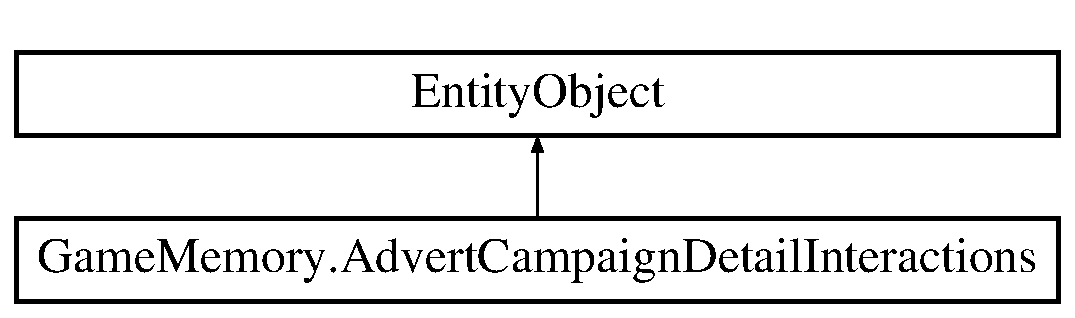
\includegraphics[height=2.000000cm]{class_game_memory_1_1_advert_campaign_detail_interactions}
\end{center}
\end{figure}
\subsection*{Static Public Member Functions}
\begin{DoxyCompactItemize}
\item 
static \\*
\hyperlink{class_game_memory_1_1_advert_campaign_detail_interactions}{Advert\-Campaign\-Detail\-Interactions} \hyperlink{class_game_memory_1_1_advert_campaign_detail_interactions_a7c7b61fe7159631078beba2c27b9d556}{Create\-Advert\-Campaign\-Detail\-Interactions} (global\-::\-System.\-Int32 advert\-Campaign\-Detail\-Interaction\-I\-D, global\-::\-System.\-Int32 advert\-I\-D, global\-::\-System.\-Decimal height, global\-::\-System.\-Date\-Time start\-Datetime)
\begin{DoxyCompactList}\small\item\em Crear un nuevo objeto \hyperlink{class_game_memory_1_1_advert_campaign_detail_interactions}{Advert\-Campaign\-Detail\-Interactions}. \end{DoxyCompactList}\end{DoxyCompactItemize}
\subsection*{Properties}
\begin{DoxyCompactItemize}
\item 
global\-::\-System.\-Int32 \hyperlink{class_game_memory_1_1_advert_campaign_detail_interactions_a15b79133fcb86178e994c495bb774593}{Advert\-Campaign\-Detail\-Interaction\-I\-D}\hspace{0.3cm}{\ttfamily  \mbox{[}get, set\mbox{]}}
\begin{DoxyCompactList}\small\item\em No hay documentación de metadatos disponible. \end{DoxyCompactList}\item 
global\-::\-System.\-Int32 \hyperlink{class_game_memory_1_1_advert_campaign_detail_interactions_af8c6dda607a3613d809d451f988b3fbe}{Advert\-I\-D}\hspace{0.3cm}{\ttfamily  \mbox{[}get, set\mbox{]}}
\begin{DoxyCompactList}\small\item\em No hay documentación de metadatos disponible. \end{DoxyCompactList}\item 
global\-::\-System.\-Decimal \hyperlink{class_game_memory_1_1_advert_campaign_detail_interactions_a10fb8d682b9d3fc999011bb92a2e44f5}{Height}\hspace{0.3cm}{\ttfamily  \mbox{[}get, set\mbox{]}}
\begin{DoxyCompactList}\small\item\em No hay documentación de metadatos disponible. \end{DoxyCompactList}\item 
Nullable$<$ global\-::\-System.\-Int32 $>$ \hyperlink{class_game_memory_1_1_advert_campaign_detail_interactions_ae756a263996a18752f44e5928792bf7a}{Time\-Elapsed}\hspace{0.3cm}{\ttfamily  \mbox{[}get, set\mbox{]}}
\begin{DoxyCompactList}\small\item\em No hay documentación de metadatos disponible. \end{DoxyCompactList}\item 
global\-::\-System.\-Date\-Time \hyperlink{class_game_memory_1_1_advert_campaign_detail_interactions_a2c4b07307a18acd8fbeb59159b8db65e}{Start\-Datetime}\hspace{0.3cm}{\ttfamily  \mbox{[}get, set\mbox{]}}
\begin{DoxyCompactList}\small\item\em No hay documentación de metadatos disponible. \end{DoxyCompactList}\item 
Nullable$<$ global\-::\-System.\-Date\-Time $>$ \hyperlink{class_game_memory_1_1_advert_campaign_detail_interactions_a9903b1858d25ea52b6a58652e38af39c}{End\-Datetime}\hspace{0.3cm}{\ttfamily  \mbox{[}get, set\mbox{]}}
\begin{DoxyCompactList}\small\item\em No hay documentación de metadatos disponible. \end{DoxyCompactList}\item 
Nullable$<$ global\-::\-System.\-Int32 $>$ \hyperlink{class_game_memory_1_1_advert_campaign_detail_interactions_a8eb103b878dc9bd2039eafba9299e467}{Advert\-Campaign\-Interaction\-\_\-\-Advert\-Campaign\-Interaction\-I\-D}\hspace{0.3cm}{\ttfamily  \mbox{[}get, set\mbox{]}}
\begin{DoxyCompactList}\small\item\em No hay documentación de metadatos disponible. \end{DoxyCompactList}\item 
\hyperlink{class_game_memory_1_1_advert_campaign_interactions}{Advert\-Campaign\-Interactions} \hyperlink{class_game_memory_1_1_advert_campaign_detail_interactions_aec05f3f3a1cd207dd87a939982dc15e9}{Advert\-Campaign\-Interactions}\hspace{0.3cm}{\ttfamily  \mbox{[}get, set\mbox{]}}
\begin{DoxyCompactList}\small\item\em No hay documentación de metadatos disponible. \end{DoxyCompactList}\item 
Entity\-Reference\\*
$<$ \hyperlink{class_game_memory_1_1_advert_campaign_interactions}{Advert\-Campaign\-Interactions} $>$ \hyperlink{class_game_memory_1_1_advert_campaign_detail_interactions_a5d502612f86f888658533cab871f3691}{Advert\-Campaign\-Interactions\-Reference}\hspace{0.3cm}{\ttfamily  \mbox{[}get, set\mbox{]}}
\begin{DoxyCompactList}\small\item\em No hay documentación de metadatos disponible. \end{DoxyCompactList}\item 
\hyperlink{class_game_memory_1_1_adverts}{Adverts} \hyperlink{class_game_memory_1_1_advert_campaign_detail_interactions_a9853269aa237b44da178e7952e73a863}{Adverts}\hspace{0.3cm}{\ttfamily  \mbox{[}get, set\mbox{]}}
\begin{DoxyCompactList}\small\item\em No hay documentación de metadatos disponible. \end{DoxyCompactList}\item 
Entity\-Reference$<$ \hyperlink{class_game_memory_1_1_adverts}{Adverts} $>$ \hyperlink{class_game_memory_1_1_advert_campaign_detail_interactions_ab65ca65f335f33f6a635a6799b48db15}{Adverts\-Reference}\hspace{0.3cm}{\ttfamily  \mbox{[}get, set\mbox{]}}
\begin{DoxyCompactList}\small\item\em No hay documentación de metadatos disponible. \end{DoxyCompactList}\end{DoxyCompactItemize}


\subsection{Detailed Description}
No hay documentación de metadatos disponible. 



\subsection{Member Function Documentation}
\hypertarget{class_game_memory_1_1_advert_campaign_detail_interactions_a7c7b61fe7159631078beba2c27b9d556}{\index{Game\-Memory\-::\-Advert\-Campaign\-Detail\-Interactions@{Game\-Memory\-::\-Advert\-Campaign\-Detail\-Interactions}!Create\-Advert\-Campaign\-Detail\-Interactions@{Create\-Advert\-Campaign\-Detail\-Interactions}}
\index{Create\-Advert\-Campaign\-Detail\-Interactions@{Create\-Advert\-Campaign\-Detail\-Interactions}!GameMemory::AdvertCampaignDetailInteractions@{Game\-Memory\-::\-Advert\-Campaign\-Detail\-Interactions}}
\subsubsection[{Create\-Advert\-Campaign\-Detail\-Interactions}]{\setlength{\rightskip}{0pt plus 5cm}static {\bf Advert\-Campaign\-Detail\-Interactions} Game\-Memory.\-Advert\-Campaign\-Detail\-Interactions.\-Create\-Advert\-Campaign\-Detail\-Interactions (
\begin{DoxyParamCaption}
\item[{global\-::\-System.\-Int32}]{advert\-Campaign\-Detail\-Interaction\-I\-D, }
\item[{global\-::\-System.\-Int32}]{advert\-I\-D, }
\item[{global\-::\-System.\-Decimal}]{height, }
\item[{global\-::\-System.\-Date\-Time}]{start\-Datetime}
\end{DoxyParamCaption}
)\hspace{0.3cm}{\ttfamily [static]}}}\label{class_game_memory_1_1_advert_campaign_detail_interactions_a7c7b61fe7159631078beba2c27b9d556}


Crear un nuevo objeto \hyperlink{class_game_memory_1_1_advert_campaign_detail_interactions}{Advert\-Campaign\-Detail\-Interactions}. 


\begin{DoxyParams}{Parameters}
{\em advert\-Campaign\-Detail\-Interaction\-I\-D} & Valor inicial de la propiedad Advert\-Campaign\-Detail\-Interaction\-I\-D.\\
\hline
{\em advert\-I\-D} & Valor inicial de la propiedad Advert\-I\-D.\\
\hline
{\em height} & Valor inicial de la propiedad Height.\\
\hline
{\em start\-Datetime} & Valor inicial de la propiedad Start\-Datetime.\\
\hline
\end{DoxyParams}


\subsection{Property Documentation}
\hypertarget{class_game_memory_1_1_advert_campaign_detail_interactions_a15b79133fcb86178e994c495bb774593}{\index{Game\-Memory\-::\-Advert\-Campaign\-Detail\-Interactions@{Game\-Memory\-::\-Advert\-Campaign\-Detail\-Interactions}!Advert\-Campaign\-Detail\-Interaction\-I\-D@{Advert\-Campaign\-Detail\-Interaction\-I\-D}}
\index{Advert\-Campaign\-Detail\-Interaction\-I\-D@{Advert\-Campaign\-Detail\-Interaction\-I\-D}!GameMemory::AdvertCampaignDetailInteractions@{Game\-Memory\-::\-Advert\-Campaign\-Detail\-Interactions}}
\subsubsection[{Advert\-Campaign\-Detail\-Interaction\-I\-D}]{\setlength{\rightskip}{0pt plus 5cm}global.\-System.\-Int32 Game\-Memory.\-Advert\-Campaign\-Detail\-Interactions.\-Advert\-Campaign\-Detail\-Interaction\-I\-D\hspace{0.3cm}{\ttfamily [get]}, {\ttfamily [set]}}}\label{class_game_memory_1_1_advert_campaign_detail_interactions_a15b79133fcb86178e994c495bb774593}


No hay documentación de metadatos disponible. 

\hypertarget{class_game_memory_1_1_advert_campaign_detail_interactions_a8eb103b878dc9bd2039eafba9299e467}{\index{Game\-Memory\-::\-Advert\-Campaign\-Detail\-Interactions@{Game\-Memory\-::\-Advert\-Campaign\-Detail\-Interactions}!Advert\-Campaign\-Interaction\-\_\-\-Advert\-Campaign\-Interaction\-I\-D@{Advert\-Campaign\-Interaction\-\_\-\-Advert\-Campaign\-Interaction\-I\-D}}
\index{Advert\-Campaign\-Interaction\-\_\-\-Advert\-Campaign\-Interaction\-I\-D@{Advert\-Campaign\-Interaction\-\_\-\-Advert\-Campaign\-Interaction\-I\-D}!GameMemory::AdvertCampaignDetailInteractions@{Game\-Memory\-::\-Advert\-Campaign\-Detail\-Interactions}}
\subsubsection[{Advert\-Campaign\-Interaction\-\_\-\-Advert\-Campaign\-Interaction\-I\-D}]{\setlength{\rightskip}{0pt plus 5cm}Nullable$<$global.\-System.\-Int32$>$ Game\-Memory.\-Advert\-Campaign\-Detail\-Interactions.\-Advert\-Campaign\-Interaction\-\_\-\-Advert\-Campaign\-Interaction\-I\-D\hspace{0.3cm}{\ttfamily [get]}, {\ttfamily [set]}}}\label{class_game_memory_1_1_advert_campaign_detail_interactions_a8eb103b878dc9bd2039eafba9299e467}


No hay documentación de metadatos disponible. 

\hypertarget{class_game_memory_1_1_advert_campaign_detail_interactions_aec05f3f3a1cd207dd87a939982dc15e9}{\index{Game\-Memory\-::\-Advert\-Campaign\-Detail\-Interactions@{Game\-Memory\-::\-Advert\-Campaign\-Detail\-Interactions}!Advert\-Campaign\-Interactions@{Advert\-Campaign\-Interactions}}
\index{Advert\-Campaign\-Interactions@{Advert\-Campaign\-Interactions}!GameMemory::AdvertCampaignDetailInteractions@{Game\-Memory\-::\-Advert\-Campaign\-Detail\-Interactions}}
\subsubsection[{Advert\-Campaign\-Interactions}]{\setlength{\rightskip}{0pt plus 5cm}{\bf Advert\-Campaign\-Interactions} Game\-Memory.\-Advert\-Campaign\-Detail\-Interactions.\-Advert\-Campaign\-Interactions\hspace{0.3cm}{\ttfamily [get]}, {\ttfamily [set]}}}\label{class_game_memory_1_1_advert_campaign_detail_interactions_aec05f3f3a1cd207dd87a939982dc15e9}


No hay documentación de metadatos disponible. 

\hypertarget{class_game_memory_1_1_advert_campaign_detail_interactions_a5d502612f86f888658533cab871f3691}{\index{Game\-Memory\-::\-Advert\-Campaign\-Detail\-Interactions@{Game\-Memory\-::\-Advert\-Campaign\-Detail\-Interactions}!Advert\-Campaign\-Interactions\-Reference@{Advert\-Campaign\-Interactions\-Reference}}
\index{Advert\-Campaign\-Interactions\-Reference@{Advert\-Campaign\-Interactions\-Reference}!GameMemory::AdvertCampaignDetailInteractions@{Game\-Memory\-::\-Advert\-Campaign\-Detail\-Interactions}}
\subsubsection[{Advert\-Campaign\-Interactions\-Reference}]{\setlength{\rightskip}{0pt plus 5cm}Entity\-Reference$<${\bf Advert\-Campaign\-Interactions}$>$ Game\-Memory.\-Advert\-Campaign\-Detail\-Interactions.\-Advert\-Campaign\-Interactions\-Reference\hspace{0.3cm}{\ttfamily [get]}, {\ttfamily [set]}}}\label{class_game_memory_1_1_advert_campaign_detail_interactions_a5d502612f86f888658533cab871f3691}


No hay documentación de metadatos disponible. 

\hypertarget{class_game_memory_1_1_advert_campaign_detail_interactions_af8c6dda607a3613d809d451f988b3fbe}{\index{Game\-Memory\-::\-Advert\-Campaign\-Detail\-Interactions@{Game\-Memory\-::\-Advert\-Campaign\-Detail\-Interactions}!Advert\-I\-D@{Advert\-I\-D}}
\index{Advert\-I\-D@{Advert\-I\-D}!GameMemory::AdvertCampaignDetailInteractions@{Game\-Memory\-::\-Advert\-Campaign\-Detail\-Interactions}}
\subsubsection[{Advert\-I\-D}]{\setlength{\rightskip}{0pt plus 5cm}global.\-System.\-Int32 Game\-Memory.\-Advert\-Campaign\-Detail\-Interactions.\-Advert\-I\-D\hspace{0.3cm}{\ttfamily [get]}, {\ttfamily [set]}}}\label{class_game_memory_1_1_advert_campaign_detail_interactions_af8c6dda607a3613d809d451f988b3fbe}


No hay documentación de metadatos disponible. 

\hypertarget{class_game_memory_1_1_advert_campaign_detail_interactions_a9853269aa237b44da178e7952e73a863}{\index{Game\-Memory\-::\-Advert\-Campaign\-Detail\-Interactions@{Game\-Memory\-::\-Advert\-Campaign\-Detail\-Interactions}!Adverts@{Adverts}}
\index{Adverts@{Adverts}!GameMemory::AdvertCampaignDetailInteractions@{Game\-Memory\-::\-Advert\-Campaign\-Detail\-Interactions}}
\subsubsection[{Adverts}]{\setlength{\rightskip}{0pt plus 5cm}{\bf Adverts} Game\-Memory.\-Advert\-Campaign\-Detail\-Interactions.\-Adverts\hspace{0.3cm}{\ttfamily [get]}, {\ttfamily [set]}}}\label{class_game_memory_1_1_advert_campaign_detail_interactions_a9853269aa237b44da178e7952e73a863}


No hay documentación de metadatos disponible. 

\hypertarget{class_game_memory_1_1_advert_campaign_detail_interactions_ab65ca65f335f33f6a635a6799b48db15}{\index{Game\-Memory\-::\-Advert\-Campaign\-Detail\-Interactions@{Game\-Memory\-::\-Advert\-Campaign\-Detail\-Interactions}!Adverts\-Reference@{Adverts\-Reference}}
\index{Adverts\-Reference@{Adverts\-Reference}!GameMemory::AdvertCampaignDetailInteractions@{Game\-Memory\-::\-Advert\-Campaign\-Detail\-Interactions}}
\subsubsection[{Adverts\-Reference}]{\setlength{\rightskip}{0pt plus 5cm}Entity\-Reference$<${\bf Adverts}$>$ Game\-Memory.\-Advert\-Campaign\-Detail\-Interactions.\-Adverts\-Reference\hspace{0.3cm}{\ttfamily [get]}, {\ttfamily [set]}}}\label{class_game_memory_1_1_advert_campaign_detail_interactions_ab65ca65f335f33f6a635a6799b48db15}


No hay documentación de metadatos disponible. 

\hypertarget{class_game_memory_1_1_advert_campaign_detail_interactions_a9903b1858d25ea52b6a58652e38af39c}{\index{Game\-Memory\-::\-Advert\-Campaign\-Detail\-Interactions@{Game\-Memory\-::\-Advert\-Campaign\-Detail\-Interactions}!End\-Datetime@{End\-Datetime}}
\index{End\-Datetime@{End\-Datetime}!GameMemory::AdvertCampaignDetailInteractions@{Game\-Memory\-::\-Advert\-Campaign\-Detail\-Interactions}}
\subsubsection[{End\-Datetime}]{\setlength{\rightskip}{0pt plus 5cm}Nullable$<$global.\-System.\-Date\-Time$>$ Game\-Memory.\-Advert\-Campaign\-Detail\-Interactions.\-End\-Datetime\hspace{0.3cm}{\ttfamily [get]}, {\ttfamily [set]}}}\label{class_game_memory_1_1_advert_campaign_detail_interactions_a9903b1858d25ea52b6a58652e38af39c}


No hay documentación de metadatos disponible. 

\hypertarget{class_game_memory_1_1_advert_campaign_detail_interactions_a10fb8d682b9d3fc999011bb92a2e44f5}{\index{Game\-Memory\-::\-Advert\-Campaign\-Detail\-Interactions@{Game\-Memory\-::\-Advert\-Campaign\-Detail\-Interactions}!Height@{Height}}
\index{Height@{Height}!GameMemory::AdvertCampaignDetailInteractions@{Game\-Memory\-::\-Advert\-Campaign\-Detail\-Interactions}}
\subsubsection[{Height}]{\setlength{\rightskip}{0pt plus 5cm}global.\-System.\-Decimal Game\-Memory.\-Advert\-Campaign\-Detail\-Interactions.\-Height\hspace{0.3cm}{\ttfamily [get]}, {\ttfamily [set]}}}\label{class_game_memory_1_1_advert_campaign_detail_interactions_a10fb8d682b9d3fc999011bb92a2e44f5}


No hay documentación de metadatos disponible. 

\hypertarget{class_game_memory_1_1_advert_campaign_detail_interactions_a2c4b07307a18acd8fbeb59159b8db65e}{\index{Game\-Memory\-::\-Advert\-Campaign\-Detail\-Interactions@{Game\-Memory\-::\-Advert\-Campaign\-Detail\-Interactions}!Start\-Datetime@{Start\-Datetime}}
\index{Start\-Datetime@{Start\-Datetime}!GameMemory::AdvertCampaignDetailInteractions@{Game\-Memory\-::\-Advert\-Campaign\-Detail\-Interactions}}
\subsubsection[{Start\-Datetime}]{\setlength{\rightskip}{0pt plus 5cm}global.\-System.\-Date\-Time Game\-Memory.\-Advert\-Campaign\-Detail\-Interactions.\-Start\-Datetime\hspace{0.3cm}{\ttfamily [get]}, {\ttfamily [set]}}}\label{class_game_memory_1_1_advert_campaign_detail_interactions_a2c4b07307a18acd8fbeb59159b8db65e}


No hay documentación de metadatos disponible. 

\hypertarget{class_game_memory_1_1_advert_campaign_detail_interactions_ae756a263996a18752f44e5928792bf7a}{\index{Game\-Memory\-::\-Advert\-Campaign\-Detail\-Interactions@{Game\-Memory\-::\-Advert\-Campaign\-Detail\-Interactions}!Time\-Elapsed@{Time\-Elapsed}}
\index{Time\-Elapsed@{Time\-Elapsed}!GameMemory::AdvertCampaignDetailInteractions@{Game\-Memory\-::\-Advert\-Campaign\-Detail\-Interactions}}
\subsubsection[{Time\-Elapsed}]{\setlength{\rightskip}{0pt plus 5cm}Nullable$<$global.\-System.\-Int32$>$ Game\-Memory.\-Advert\-Campaign\-Detail\-Interactions.\-Time\-Elapsed\hspace{0.3cm}{\ttfamily [get]}, {\ttfamily [set]}}}\label{class_game_memory_1_1_advert_campaign_detail_interactions_ae756a263996a18752f44e5928792bf7a}


No hay documentación de metadatos disponible. 



The documentation for this class was generated from the following file\-:\begin{DoxyCompactItemize}
\item 
D\-:/tesis\-Assembla/branches/\-Branch\-\_\-\-Tesis\-\_\-\-Sprint01/\-Dev/\-Interaction Module/\-Game\-Memory/\-Game\-Memory/O\-M\-K\-T.\-Designer.\-cs\end{DoxyCompactItemize}

\hypertarget{class_game_memory_1_1_advert_campaign_details}{\section{Game\-Memory.\-Advert\-Campaign\-Details Class Reference}
\label{class_game_memory_1_1_advert_campaign_details}\index{Game\-Memory.\-Advert\-Campaign\-Details@{Game\-Memory.\-Advert\-Campaign\-Details}}
}


No hay documentación de metadatos disponible.  


Inheritance diagram for Game\-Memory.\-Advert\-Campaign\-Details\-:\begin{figure}[H]
\begin{center}
\leavevmode
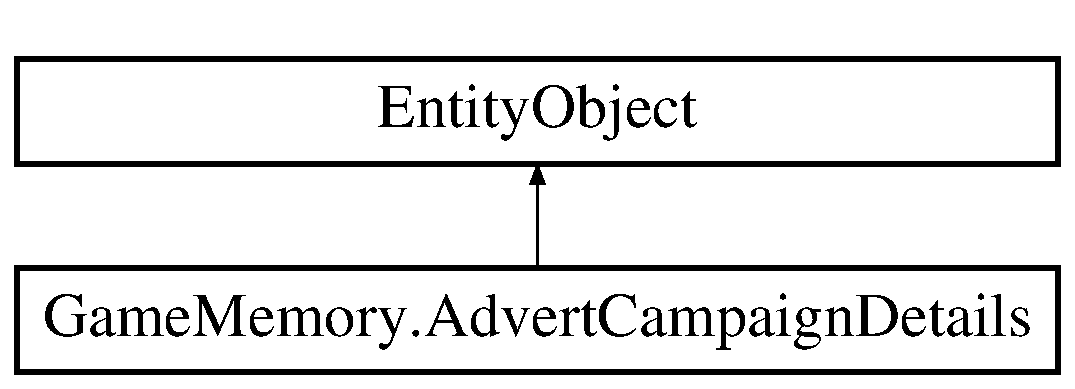
\includegraphics[height=2.000000cm]{class_game_memory_1_1_advert_campaign_details}
\end{center}
\end{figure}
\subsection*{Static Public Member Functions}
\begin{DoxyCompactItemize}
\item 
static \hyperlink{class_game_memory_1_1_advert_campaign_details}{Advert\-Campaign\-Details} \hyperlink{class_game_memory_1_1_advert_campaign_details_ac69bee7e775bf7dcc7d5461189198b8b}{Create\-Advert\-Campaign\-Details} (global\-::\-System.\-Int32 advert\-Campaign\-Detail\-Id, global\-::\-System.\-Int32 advert\-Campaign\-Id, global\-::\-System.\-Int32 advert\-I\-D)
\begin{DoxyCompactList}\small\item\em Crear un nuevo objeto \hyperlink{class_game_memory_1_1_advert_campaign_details}{Advert\-Campaign\-Details}. \end{DoxyCompactList}\end{DoxyCompactItemize}
\subsection*{Properties}
\begin{DoxyCompactItemize}
\item 
global\-::\-System.\-Int32 \hyperlink{class_game_memory_1_1_advert_campaign_details_a8c0831e7c4ad9024c34271fea79ce567}{Advert\-Campaign\-Detail\-Id}\hspace{0.3cm}{\ttfamily  \mbox{[}get, set\mbox{]}}
\begin{DoxyCompactList}\small\item\em No hay documentación de metadatos disponible. \end{DoxyCompactList}\item 
Nullable$<$ global\-::\-System.\-Date\-Time $>$ \hyperlink{class_game_memory_1_1_advert_campaign_details_a22a86c021a8119defac4074a13bbb1e3}{End\-Date}\hspace{0.3cm}{\ttfamily  \mbox{[}get, set\mbox{]}}
\begin{DoxyCompactList}\small\item\em No hay documentación de metadatos disponible. \end{DoxyCompactList}\item 
Nullable$<$ global\-::\-System.\-Date\-Time $>$ \hyperlink{class_game_memory_1_1_advert_campaign_details_a944d2e6fa9b724a2a2c6dcc83435c943}{Start\-Date}\hspace{0.3cm}{\ttfamily  \mbox{[}get, set\mbox{]}}
\begin{DoxyCompactList}\small\item\em No hay documentación de metadatos disponible. \end{DoxyCompactList}\item 
global\-::\-System.\-String \hyperlink{class_game_memory_1_1_advert_campaign_details_a95b6b6def95516b545e5ba17431a1a6e}{Advert\-Group}\hspace{0.3cm}{\ttfamily  \mbox{[}get, set\mbox{]}}
\begin{DoxyCompactList}\small\item\em No hay documentación de metadatos disponible. \end{DoxyCompactList}\item 
global\-::\-System.\-Int32 \hyperlink{class_game_memory_1_1_advert_campaign_details_afa3d0399d1018143dabdf96501e5df3d}{Advert\-Campaign\-Id}\hspace{0.3cm}{\ttfamily  \mbox{[}get, set\mbox{]}}
\begin{DoxyCompactList}\small\item\em No hay documentación de metadatos disponible. \end{DoxyCompactList}\item 
global\-::\-System.\-Int32 \hyperlink{class_game_memory_1_1_advert_campaign_details_a322157e3435d7d1ff384fc2fc60b5656}{Advert\-I\-D}\hspace{0.3cm}{\ttfamily  \mbox{[}get, set\mbox{]}}
\begin{DoxyCompactList}\small\item\em No hay documentación de metadatos disponible. \end{DoxyCompactList}\item 
\hyperlink{class_game_memory_1_1_advert_campaigns}{Advert\-Campaigns} \hyperlink{class_game_memory_1_1_advert_campaign_details_afbf36c0e9f7113d2b946475ab0ff95df}{Advert\-Campaigns}\hspace{0.3cm}{\ttfamily  \mbox{[}get, set\mbox{]}}
\begin{DoxyCompactList}\small\item\em No hay documentación de metadatos disponible. \end{DoxyCompactList}\item 
Entity\-Reference$<$ \hyperlink{class_game_memory_1_1_advert_campaigns}{Advert\-Campaigns} $>$ \hyperlink{class_game_memory_1_1_advert_campaign_details_aa7b63926aba9be6e0a00d3f3f666f13c}{Advert\-Campaigns\-Reference}\hspace{0.3cm}{\ttfamily  \mbox{[}get, set\mbox{]}}
\begin{DoxyCompactList}\small\item\em No hay documentación de metadatos disponible. \end{DoxyCompactList}\item 
\hyperlink{class_game_memory_1_1_adverts}{Adverts} \hyperlink{class_game_memory_1_1_advert_campaign_details_a9abbe4e8fd98bab4accdc80aa19afbc9}{Adverts}\hspace{0.3cm}{\ttfamily  \mbox{[}get, set\mbox{]}}
\begin{DoxyCompactList}\small\item\em No hay documentación de metadatos disponible. \end{DoxyCompactList}\item 
Entity\-Reference$<$ \hyperlink{class_game_memory_1_1_adverts}{Adverts} $>$ \hyperlink{class_game_memory_1_1_advert_campaign_details_ac0bd4032d1453cc94b31066b61da0e3c}{Adverts\-Reference}\hspace{0.3cm}{\ttfamily  \mbox{[}get, set\mbox{]}}
\begin{DoxyCompactList}\small\item\em No hay documentación de metadatos disponible. \end{DoxyCompactList}\item 
Entity\-Collection$<$ \hyperlink{class_game_memory_1_1_interactions}{Interactions} $>$ \hyperlink{class_game_memory_1_1_advert_campaign_details_aed4bd9e4877c0af4c00f36a578213ac0}{Interactions}\hspace{0.3cm}{\ttfamily  \mbox{[}get, set\mbox{]}}
\begin{DoxyCompactList}\small\item\em No hay documentación de metadatos disponible. \end{DoxyCompactList}\end{DoxyCompactItemize}


\subsection{Detailed Description}
No hay documentación de metadatos disponible. 



\subsection{Member Function Documentation}
\hypertarget{class_game_memory_1_1_advert_campaign_details_ac69bee7e775bf7dcc7d5461189198b8b}{\index{Game\-Memory\-::\-Advert\-Campaign\-Details@{Game\-Memory\-::\-Advert\-Campaign\-Details}!Create\-Advert\-Campaign\-Details@{Create\-Advert\-Campaign\-Details}}
\index{Create\-Advert\-Campaign\-Details@{Create\-Advert\-Campaign\-Details}!GameMemory::AdvertCampaignDetails@{Game\-Memory\-::\-Advert\-Campaign\-Details}}
\subsubsection[{Create\-Advert\-Campaign\-Details}]{\setlength{\rightskip}{0pt plus 5cm}static {\bf Advert\-Campaign\-Details} Game\-Memory.\-Advert\-Campaign\-Details.\-Create\-Advert\-Campaign\-Details (
\begin{DoxyParamCaption}
\item[{global\-::\-System.\-Int32}]{advert\-Campaign\-Detail\-Id, }
\item[{global\-::\-System.\-Int32}]{advert\-Campaign\-Id, }
\item[{global\-::\-System.\-Int32}]{advert\-I\-D}
\end{DoxyParamCaption}
)\hspace{0.3cm}{\ttfamily [static]}}}\label{class_game_memory_1_1_advert_campaign_details_ac69bee7e775bf7dcc7d5461189198b8b}


Crear un nuevo objeto \hyperlink{class_game_memory_1_1_advert_campaign_details}{Advert\-Campaign\-Details}. 


\begin{DoxyParams}{Parameters}
{\em advert\-Campaign\-Detail\-Id} & Valor inicial de la propiedad Advert\-Campaign\-Detail\-Id.\\
\hline
{\em advert\-Campaign\-Id} & Valor inicial de la propiedad Advert\-Campaign\-Id.\\
\hline
{\em advert\-I\-D} & Valor inicial de la propiedad Advert\-I\-D.\\
\hline
\end{DoxyParams}


\subsection{Property Documentation}
\hypertarget{class_game_memory_1_1_advert_campaign_details_a8c0831e7c4ad9024c34271fea79ce567}{\index{Game\-Memory\-::\-Advert\-Campaign\-Details@{Game\-Memory\-::\-Advert\-Campaign\-Details}!Advert\-Campaign\-Detail\-Id@{Advert\-Campaign\-Detail\-Id}}
\index{Advert\-Campaign\-Detail\-Id@{Advert\-Campaign\-Detail\-Id}!GameMemory::AdvertCampaignDetails@{Game\-Memory\-::\-Advert\-Campaign\-Details}}
\subsubsection[{Advert\-Campaign\-Detail\-Id}]{\setlength{\rightskip}{0pt plus 5cm}global.\-System.\-Int32 Game\-Memory.\-Advert\-Campaign\-Details.\-Advert\-Campaign\-Detail\-Id\hspace{0.3cm}{\ttfamily [get]}, {\ttfamily [set]}}}\label{class_game_memory_1_1_advert_campaign_details_a8c0831e7c4ad9024c34271fea79ce567}


No hay documentación de metadatos disponible. 

\hypertarget{class_game_memory_1_1_advert_campaign_details_afa3d0399d1018143dabdf96501e5df3d}{\index{Game\-Memory\-::\-Advert\-Campaign\-Details@{Game\-Memory\-::\-Advert\-Campaign\-Details}!Advert\-Campaign\-Id@{Advert\-Campaign\-Id}}
\index{Advert\-Campaign\-Id@{Advert\-Campaign\-Id}!GameMemory::AdvertCampaignDetails@{Game\-Memory\-::\-Advert\-Campaign\-Details}}
\subsubsection[{Advert\-Campaign\-Id}]{\setlength{\rightskip}{0pt plus 5cm}global.\-System.\-Int32 Game\-Memory.\-Advert\-Campaign\-Details.\-Advert\-Campaign\-Id\hspace{0.3cm}{\ttfamily [get]}, {\ttfamily [set]}}}\label{class_game_memory_1_1_advert_campaign_details_afa3d0399d1018143dabdf96501e5df3d}


No hay documentación de metadatos disponible. 

\hypertarget{class_game_memory_1_1_advert_campaign_details_afbf36c0e9f7113d2b946475ab0ff95df}{\index{Game\-Memory\-::\-Advert\-Campaign\-Details@{Game\-Memory\-::\-Advert\-Campaign\-Details}!Advert\-Campaigns@{Advert\-Campaigns}}
\index{Advert\-Campaigns@{Advert\-Campaigns}!GameMemory::AdvertCampaignDetails@{Game\-Memory\-::\-Advert\-Campaign\-Details}}
\subsubsection[{Advert\-Campaigns}]{\setlength{\rightskip}{0pt plus 5cm}{\bf Advert\-Campaigns} Game\-Memory.\-Advert\-Campaign\-Details.\-Advert\-Campaigns\hspace{0.3cm}{\ttfamily [get]}, {\ttfamily [set]}}}\label{class_game_memory_1_1_advert_campaign_details_afbf36c0e9f7113d2b946475ab0ff95df}


No hay documentación de metadatos disponible. 

\hypertarget{class_game_memory_1_1_advert_campaign_details_aa7b63926aba9be6e0a00d3f3f666f13c}{\index{Game\-Memory\-::\-Advert\-Campaign\-Details@{Game\-Memory\-::\-Advert\-Campaign\-Details}!Advert\-Campaigns\-Reference@{Advert\-Campaigns\-Reference}}
\index{Advert\-Campaigns\-Reference@{Advert\-Campaigns\-Reference}!GameMemory::AdvertCampaignDetails@{Game\-Memory\-::\-Advert\-Campaign\-Details}}
\subsubsection[{Advert\-Campaigns\-Reference}]{\setlength{\rightskip}{0pt plus 5cm}Entity\-Reference$<${\bf Advert\-Campaigns}$>$ Game\-Memory.\-Advert\-Campaign\-Details.\-Advert\-Campaigns\-Reference\hspace{0.3cm}{\ttfamily [get]}, {\ttfamily [set]}}}\label{class_game_memory_1_1_advert_campaign_details_aa7b63926aba9be6e0a00d3f3f666f13c}


No hay documentación de metadatos disponible. 

\hypertarget{class_game_memory_1_1_advert_campaign_details_a95b6b6def95516b545e5ba17431a1a6e}{\index{Game\-Memory\-::\-Advert\-Campaign\-Details@{Game\-Memory\-::\-Advert\-Campaign\-Details}!Advert\-Group@{Advert\-Group}}
\index{Advert\-Group@{Advert\-Group}!GameMemory::AdvertCampaignDetails@{Game\-Memory\-::\-Advert\-Campaign\-Details}}
\subsubsection[{Advert\-Group}]{\setlength{\rightskip}{0pt plus 5cm}global.\-System.\-String Game\-Memory.\-Advert\-Campaign\-Details.\-Advert\-Group\hspace{0.3cm}{\ttfamily [get]}, {\ttfamily [set]}}}\label{class_game_memory_1_1_advert_campaign_details_a95b6b6def95516b545e5ba17431a1a6e}


No hay documentación de metadatos disponible. 

\hypertarget{class_game_memory_1_1_advert_campaign_details_a322157e3435d7d1ff384fc2fc60b5656}{\index{Game\-Memory\-::\-Advert\-Campaign\-Details@{Game\-Memory\-::\-Advert\-Campaign\-Details}!Advert\-I\-D@{Advert\-I\-D}}
\index{Advert\-I\-D@{Advert\-I\-D}!GameMemory::AdvertCampaignDetails@{Game\-Memory\-::\-Advert\-Campaign\-Details}}
\subsubsection[{Advert\-I\-D}]{\setlength{\rightskip}{0pt plus 5cm}global.\-System.\-Int32 Game\-Memory.\-Advert\-Campaign\-Details.\-Advert\-I\-D\hspace{0.3cm}{\ttfamily [get]}, {\ttfamily [set]}}}\label{class_game_memory_1_1_advert_campaign_details_a322157e3435d7d1ff384fc2fc60b5656}


No hay documentación de metadatos disponible. 

\hypertarget{class_game_memory_1_1_advert_campaign_details_a9abbe4e8fd98bab4accdc80aa19afbc9}{\index{Game\-Memory\-::\-Advert\-Campaign\-Details@{Game\-Memory\-::\-Advert\-Campaign\-Details}!Adverts@{Adverts}}
\index{Adverts@{Adverts}!GameMemory::AdvertCampaignDetails@{Game\-Memory\-::\-Advert\-Campaign\-Details}}
\subsubsection[{Adverts}]{\setlength{\rightskip}{0pt plus 5cm}{\bf Adverts} Game\-Memory.\-Advert\-Campaign\-Details.\-Adverts\hspace{0.3cm}{\ttfamily [get]}, {\ttfamily [set]}}}\label{class_game_memory_1_1_advert_campaign_details_a9abbe4e8fd98bab4accdc80aa19afbc9}


No hay documentación de metadatos disponible. 

\hypertarget{class_game_memory_1_1_advert_campaign_details_ac0bd4032d1453cc94b31066b61da0e3c}{\index{Game\-Memory\-::\-Advert\-Campaign\-Details@{Game\-Memory\-::\-Advert\-Campaign\-Details}!Adverts\-Reference@{Adverts\-Reference}}
\index{Adverts\-Reference@{Adverts\-Reference}!GameMemory::AdvertCampaignDetails@{Game\-Memory\-::\-Advert\-Campaign\-Details}}
\subsubsection[{Adverts\-Reference}]{\setlength{\rightskip}{0pt plus 5cm}Entity\-Reference$<${\bf Adverts}$>$ Game\-Memory.\-Advert\-Campaign\-Details.\-Adverts\-Reference\hspace{0.3cm}{\ttfamily [get]}, {\ttfamily [set]}}}\label{class_game_memory_1_1_advert_campaign_details_ac0bd4032d1453cc94b31066b61da0e3c}


No hay documentación de metadatos disponible. 

\hypertarget{class_game_memory_1_1_advert_campaign_details_a22a86c021a8119defac4074a13bbb1e3}{\index{Game\-Memory\-::\-Advert\-Campaign\-Details@{Game\-Memory\-::\-Advert\-Campaign\-Details}!End\-Date@{End\-Date}}
\index{End\-Date@{End\-Date}!GameMemory::AdvertCampaignDetails@{Game\-Memory\-::\-Advert\-Campaign\-Details}}
\subsubsection[{End\-Date}]{\setlength{\rightskip}{0pt plus 5cm}Nullable$<$global.\-System.\-Date\-Time$>$ Game\-Memory.\-Advert\-Campaign\-Details.\-End\-Date\hspace{0.3cm}{\ttfamily [get]}, {\ttfamily [set]}}}\label{class_game_memory_1_1_advert_campaign_details_a22a86c021a8119defac4074a13bbb1e3}


No hay documentación de metadatos disponible. 

\hypertarget{class_game_memory_1_1_advert_campaign_details_aed4bd9e4877c0af4c00f36a578213ac0}{\index{Game\-Memory\-::\-Advert\-Campaign\-Details@{Game\-Memory\-::\-Advert\-Campaign\-Details}!Interactions@{Interactions}}
\index{Interactions@{Interactions}!GameMemory::AdvertCampaignDetails@{Game\-Memory\-::\-Advert\-Campaign\-Details}}
\subsubsection[{Interactions}]{\setlength{\rightskip}{0pt plus 5cm}Entity\-Collection$<${\bf Interactions}$>$ Game\-Memory.\-Advert\-Campaign\-Details.\-Interactions\hspace{0.3cm}{\ttfamily [get]}, {\ttfamily [set]}}}\label{class_game_memory_1_1_advert_campaign_details_aed4bd9e4877c0af4c00f36a578213ac0}


No hay documentación de metadatos disponible. 

\hypertarget{class_game_memory_1_1_advert_campaign_details_a944d2e6fa9b724a2a2c6dcc83435c943}{\index{Game\-Memory\-::\-Advert\-Campaign\-Details@{Game\-Memory\-::\-Advert\-Campaign\-Details}!Start\-Date@{Start\-Date}}
\index{Start\-Date@{Start\-Date}!GameMemory::AdvertCampaignDetails@{Game\-Memory\-::\-Advert\-Campaign\-Details}}
\subsubsection[{Start\-Date}]{\setlength{\rightskip}{0pt plus 5cm}Nullable$<$global.\-System.\-Date\-Time$>$ Game\-Memory.\-Advert\-Campaign\-Details.\-Start\-Date\hspace{0.3cm}{\ttfamily [get]}, {\ttfamily [set]}}}\label{class_game_memory_1_1_advert_campaign_details_a944d2e6fa9b724a2a2c6dcc83435c943}


No hay documentación de metadatos disponible. 



The documentation for this class was generated from the following file\-:\begin{DoxyCompactItemize}
\item 
D\-:/tesis\-Assembla/branches/\-Branch\-\_\-\-Tesis\-\_\-\-Sprint01/\-Dev/\-Interaction Module/\-Game\-Memory/\-Game\-Memory/O\-M\-K\-T.\-Designer.\-cs\end{DoxyCompactItemize}

\hypertarget{class_game_memory_1_1_advert_campaign_interactions}{\section{Game\-Memory.\-Advert\-Campaign\-Interactions Class Reference}
\label{class_game_memory_1_1_advert_campaign_interactions}\index{Game\-Memory.\-Advert\-Campaign\-Interactions@{Game\-Memory.\-Advert\-Campaign\-Interactions}}
}


No hay documentación de metadatos disponible.  


Inheritance diagram for Game\-Memory.\-Advert\-Campaign\-Interactions\-:\begin{figure}[H]
\begin{center}
\leavevmode
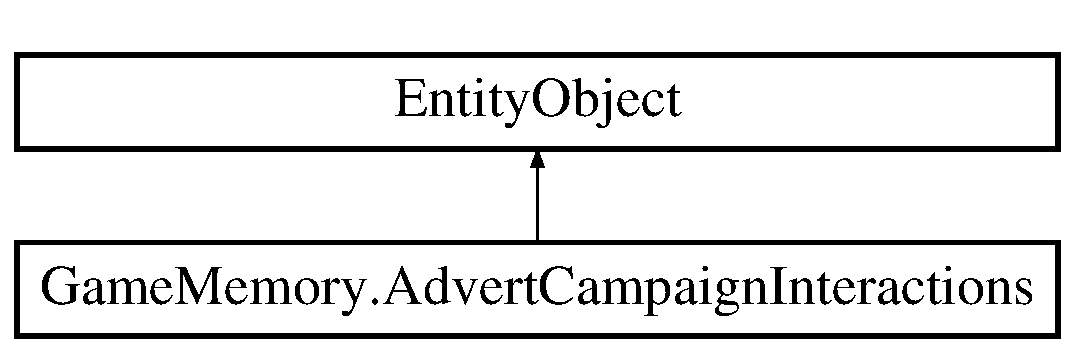
\includegraphics[height=2.000000cm]{class_game_memory_1_1_advert_campaign_interactions}
\end{center}
\end{figure}
\subsection*{Static Public Member Functions}
\begin{DoxyCompactItemize}
\item 
static \hyperlink{class_game_memory_1_1_advert_campaign_interactions}{Advert\-Campaign\-Interactions} \hyperlink{class_game_memory_1_1_advert_campaign_interactions_a6a464a87734cfdc93b4cb680fa745f9b}{Create\-Advert\-Campaign\-Interactions} (global\-::\-System.\-Int32 advert\-Campaign\-Interaction\-I\-D, global\-::\-System.\-Int32 advert\-Campaign\-I\-D, global\-::\-System.\-Date\-Time start\-Datetime)
\begin{DoxyCompactList}\small\item\em Crear un nuevo objeto \hyperlink{class_game_memory_1_1_advert_campaign_interactions}{Advert\-Campaign\-Interactions}. \end{DoxyCompactList}\end{DoxyCompactItemize}
\subsection*{Properties}
\begin{DoxyCompactItemize}
\item 
global\-::\-System.\-Int32 \hyperlink{class_game_memory_1_1_advert_campaign_interactions_a100229f66f8386d876b9ae09a16e2b2d}{Advert\-Campaign\-Interaction\-I\-D}\hspace{0.3cm}{\ttfamily  \mbox{[}get, set\mbox{]}}
\begin{DoxyCompactList}\small\item\em No hay documentación de metadatos disponible. \end{DoxyCompactList}\item 
global\-::\-System.\-Int32 \hyperlink{class_game_memory_1_1_advert_campaign_interactions_a1f5ba2d040aee7f7c01dcec6e48cf4d0}{Advert\-Campaign\-I\-D}\hspace{0.3cm}{\ttfamily  \mbox{[}get, set\mbox{]}}
\begin{DoxyCompactList}\small\item\em No hay documentación de metadatos disponible. \end{DoxyCompactList}\item 
global\-::\-System.\-Date\-Time \hyperlink{class_game_memory_1_1_advert_campaign_interactions_ab45778d100a4712092c7e4596a0f202b}{Start\-Datetime}\hspace{0.3cm}{\ttfamily  \mbox{[}get, set\mbox{]}}
\begin{DoxyCompactList}\small\item\em No hay documentación de metadatos disponible. \end{DoxyCompactList}\item 
Nullable$<$ global\-::\-System.\-Date\-Time $>$ \hyperlink{class_game_memory_1_1_advert_campaign_interactions_ab6ed1c939196344d74d443aca721c5e1}{End\-Datetime}\hspace{0.3cm}{\ttfamily  \mbox{[}get, set\mbox{]}}
\begin{DoxyCompactList}\small\item\em No hay documentación de metadatos disponible. \end{DoxyCompactList}\item 
Nullable$<$ global\-::\-System.\-Int32 $>$ \hyperlink{class_game_memory_1_1_advert_campaign_interactions_a7bd92a415be6927712becae96824e73d}{Time\-Elapsed}\hspace{0.3cm}{\ttfamily  \mbox{[}get, set\mbox{]}}
\begin{DoxyCompactList}\small\item\em No hay documentación de metadatos disponible. \end{DoxyCompactList}\item 
Entity\-Collection\\*
$<$ \hyperlink{class_game_memory_1_1_advert_campaign_detail_interactions}{Advert\-Campaign\-Detail\-Interactions} $>$ \hyperlink{class_game_memory_1_1_advert_campaign_interactions_a76c26241b44be34ad0751c279509b2f3}{Advert\-Campaign\-Detail\-Interactions}\hspace{0.3cm}{\ttfamily  \mbox{[}get, set\mbox{]}}
\begin{DoxyCompactList}\small\item\em No hay documentación de metadatos disponible. \end{DoxyCompactList}\item 
\hyperlink{class_game_memory_1_1_advert_campaigns}{Advert\-Campaigns} \hyperlink{class_game_memory_1_1_advert_campaign_interactions_a74c28d9fcf8c849a43a99292cfea1176}{Advert\-Campaigns}\hspace{0.3cm}{\ttfamily  \mbox{[}get, set\mbox{]}}
\begin{DoxyCompactList}\small\item\em No hay documentación de metadatos disponible. \end{DoxyCompactList}\item 
Entity\-Reference$<$ \hyperlink{class_game_memory_1_1_advert_campaigns}{Advert\-Campaigns} $>$ \hyperlink{class_game_memory_1_1_advert_campaign_interactions_ab12596b7807a0658f0198e535a33ef2f}{Advert\-Campaigns\-Reference}\hspace{0.3cm}{\ttfamily  \mbox{[}get, set\mbox{]}}
\begin{DoxyCompactList}\small\item\em No hay documentación de metadatos disponible. \end{DoxyCompactList}\end{DoxyCompactItemize}


\subsection{Detailed Description}
No hay documentación de metadatos disponible. 



\subsection{Member Function Documentation}
\hypertarget{class_game_memory_1_1_advert_campaign_interactions_a6a464a87734cfdc93b4cb680fa745f9b}{\index{Game\-Memory\-::\-Advert\-Campaign\-Interactions@{Game\-Memory\-::\-Advert\-Campaign\-Interactions}!Create\-Advert\-Campaign\-Interactions@{Create\-Advert\-Campaign\-Interactions}}
\index{Create\-Advert\-Campaign\-Interactions@{Create\-Advert\-Campaign\-Interactions}!GameMemory::AdvertCampaignInteractions@{Game\-Memory\-::\-Advert\-Campaign\-Interactions}}
\subsubsection[{Create\-Advert\-Campaign\-Interactions}]{\setlength{\rightskip}{0pt plus 5cm}static {\bf Advert\-Campaign\-Interactions} Game\-Memory.\-Advert\-Campaign\-Interactions.\-Create\-Advert\-Campaign\-Interactions (
\begin{DoxyParamCaption}
\item[{global\-::\-System.\-Int32}]{advert\-Campaign\-Interaction\-I\-D, }
\item[{global\-::\-System.\-Int32}]{advert\-Campaign\-I\-D, }
\item[{global\-::\-System.\-Date\-Time}]{start\-Datetime}
\end{DoxyParamCaption}
)\hspace{0.3cm}{\ttfamily [static]}}}\label{class_game_memory_1_1_advert_campaign_interactions_a6a464a87734cfdc93b4cb680fa745f9b}


Crear un nuevo objeto \hyperlink{class_game_memory_1_1_advert_campaign_interactions}{Advert\-Campaign\-Interactions}. 


\begin{DoxyParams}{Parameters}
{\em advert\-Campaign\-Interaction\-I\-D} & Valor inicial de la propiedad Advert\-Campaign\-Interaction\-I\-D.\\
\hline
{\em advert\-Campaign\-I\-D} & Valor inicial de la propiedad Advert\-Campaign\-I\-D.\\
\hline
{\em start\-Datetime} & Valor inicial de la propiedad Start\-Datetime.\\
\hline
\end{DoxyParams}


\subsection{Property Documentation}
\hypertarget{class_game_memory_1_1_advert_campaign_interactions_a76c26241b44be34ad0751c279509b2f3}{\index{Game\-Memory\-::\-Advert\-Campaign\-Interactions@{Game\-Memory\-::\-Advert\-Campaign\-Interactions}!Advert\-Campaign\-Detail\-Interactions@{Advert\-Campaign\-Detail\-Interactions}}
\index{Advert\-Campaign\-Detail\-Interactions@{Advert\-Campaign\-Detail\-Interactions}!GameMemory::AdvertCampaignInteractions@{Game\-Memory\-::\-Advert\-Campaign\-Interactions}}
\subsubsection[{Advert\-Campaign\-Detail\-Interactions}]{\setlength{\rightskip}{0pt plus 5cm}Entity\-Collection$<${\bf Advert\-Campaign\-Detail\-Interactions}$>$ Game\-Memory.\-Advert\-Campaign\-Interactions.\-Advert\-Campaign\-Detail\-Interactions\hspace{0.3cm}{\ttfamily [get]}, {\ttfamily [set]}}}\label{class_game_memory_1_1_advert_campaign_interactions_a76c26241b44be34ad0751c279509b2f3}


No hay documentación de metadatos disponible. 

\hypertarget{class_game_memory_1_1_advert_campaign_interactions_a1f5ba2d040aee7f7c01dcec6e48cf4d0}{\index{Game\-Memory\-::\-Advert\-Campaign\-Interactions@{Game\-Memory\-::\-Advert\-Campaign\-Interactions}!Advert\-Campaign\-I\-D@{Advert\-Campaign\-I\-D}}
\index{Advert\-Campaign\-I\-D@{Advert\-Campaign\-I\-D}!GameMemory::AdvertCampaignInteractions@{Game\-Memory\-::\-Advert\-Campaign\-Interactions}}
\subsubsection[{Advert\-Campaign\-I\-D}]{\setlength{\rightskip}{0pt plus 5cm}global.\-System.\-Int32 Game\-Memory.\-Advert\-Campaign\-Interactions.\-Advert\-Campaign\-I\-D\hspace{0.3cm}{\ttfamily [get]}, {\ttfamily [set]}}}\label{class_game_memory_1_1_advert_campaign_interactions_a1f5ba2d040aee7f7c01dcec6e48cf4d0}


No hay documentación de metadatos disponible. 

\hypertarget{class_game_memory_1_1_advert_campaign_interactions_a100229f66f8386d876b9ae09a16e2b2d}{\index{Game\-Memory\-::\-Advert\-Campaign\-Interactions@{Game\-Memory\-::\-Advert\-Campaign\-Interactions}!Advert\-Campaign\-Interaction\-I\-D@{Advert\-Campaign\-Interaction\-I\-D}}
\index{Advert\-Campaign\-Interaction\-I\-D@{Advert\-Campaign\-Interaction\-I\-D}!GameMemory::AdvertCampaignInteractions@{Game\-Memory\-::\-Advert\-Campaign\-Interactions}}
\subsubsection[{Advert\-Campaign\-Interaction\-I\-D}]{\setlength{\rightskip}{0pt plus 5cm}global.\-System.\-Int32 Game\-Memory.\-Advert\-Campaign\-Interactions.\-Advert\-Campaign\-Interaction\-I\-D\hspace{0.3cm}{\ttfamily [get]}, {\ttfamily [set]}}}\label{class_game_memory_1_1_advert_campaign_interactions_a100229f66f8386d876b9ae09a16e2b2d}


No hay documentación de metadatos disponible. 

\hypertarget{class_game_memory_1_1_advert_campaign_interactions_a74c28d9fcf8c849a43a99292cfea1176}{\index{Game\-Memory\-::\-Advert\-Campaign\-Interactions@{Game\-Memory\-::\-Advert\-Campaign\-Interactions}!Advert\-Campaigns@{Advert\-Campaigns}}
\index{Advert\-Campaigns@{Advert\-Campaigns}!GameMemory::AdvertCampaignInteractions@{Game\-Memory\-::\-Advert\-Campaign\-Interactions}}
\subsubsection[{Advert\-Campaigns}]{\setlength{\rightskip}{0pt plus 5cm}{\bf Advert\-Campaigns} Game\-Memory.\-Advert\-Campaign\-Interactions.\-Advert\-Campaigns\hspace{0.3cm}{\ttfamily [get]}, {\ttfamily [set]}}}\label{class_game_memory_1_1_advert_campaign_interactions_a74c28d9fcf8c849a43a99292cfea1176}


No hay documentación de metadatos disponible. 

\hypertarget{class_game_memory_1_1_advert_campaign_interactions_ab12596b7807a0658f0198e535a33ef2f}{\index{Game\-Memory\-::\-Advert\-Campaign\-Interactions@{Game\-Memory\-::\-Advert\-Campaign\-Interactions}!Advert\-Campaigns\-Reference@{Advert\-Campaigns\-Reference}}
\index{Advert\-Campaigns\-Reference@{Advert\-Campaigns\-Reference}!GameMemory::AdvertCampaignInteractions@{Game\-Memory\-::\-Advert\-Campaign\-Interactions}}
\subsubsection[{Advert\-Campaigns\-Reference}]{\setlength{\rightskip}{0pt plus 5cm}Entity\-Reference$<${\bf Advert\-Campaigns}$>$ Game\-Memory.\-Advert\-Campaign\-Interactions.\-Advert\-Campaigns\-Reference\hspace{0.3cm}{\ttfamily [get]}, {\ttfamily [set]}}}\label{class_game_memory_1_1_advert_campaign_interactions_ab12596b7807a0658f0198e535a33ef2f}


No hay documentación de metadatos disponible. 

\hypertarget{class_game_memory_1_1_advert_campaign_interactions_ab6ed1c939196344d74d443aca721c5e1}{\index{Game\-Memory\-::\-Advert\-Campaign\-Interactions@{Game\-Memory\-::\-Advert\-Campaign\-Interactions}!End\-Datetime@{End\-Datetime}}
\index{End\-Datetime@{End\-Datetime}!GameMemory::AdvertCampaignInteractions@{Game\-Memory\-::\-Advert\-Campaign\-Interactions}}
\subsubsection[{End\-Datetime}]{\setlength{\rightskip}{0pt plus 5cm}Nullable$<$global.\-System.\-Date\-Time$>$ Game\-Memory.\-Advert\-Campaign\-Interactions.\-End\-Datetime\hspace{0.3cm}{\ttfamily [get]}, {\ttfamily [set]}}}\label{class_game_memory_1_1_advert_campaign_interactions_ab6ed1c939196344d74d443aca721c5e1}


No hay documentación de metadatos disponible. 

\hypertarget{class_game_memory_1_1_advert_campaign_interactions_ab45778d100a4712092c7e4596a0f202b}{\index{Game\-Memory\-::\-Advert\-Campaign\-Interactions@{Game\-Memory\-::\-Advert\-Campaign\-Interactions}!Start\-Datetime@{Start\-Datetime}}
\index{Start\-Datetime@{Start\-Datetime}!GameMemory::AdvertCampaignInteractions@{Game\-Memory\-::\-Advert\-Campaign\-Interactions}}
\subsubsection[{Start\-Datetime}]{\setlength{\rightskip}{0pt plus 5cm}global.\-System.\-Date\-Time Game\-Memory.\-Advert\-Campaign\-Interactions.\-Start\-Datetime\hspace{0.3cm}{\ttfamily [get]}, {\ttfamily [set]}}}\label{class_game_memory_1_1_advert_campaign_interactions_ab45778d100a4712092c7e4596a0f202b}


No hay documentación de metadatos disponible. 

\hypertarget{class_game_memory_1_1_advert_campaign_interactions_a7bd92a415be6927712becae96824e73d}{\index{Game\-Memory\-::\-Advert\-Campaign\-Interactions@{Game\-Memory\-::\-Advert\-Campaign\-Interactions}!Time\-Elapsed@{Time\-Elapsed}}
\index{Time\-Elapsed@{Time\-Elapsed}!GameMemory::AdvertCampaignInteractions@{Game\-Memory\-::\-Advert\-Campaign\-Interactions}}
\subsubsection[{Time\-Elapsed}]{\setlength{\rightskip}{0pt plus 5cm}Nullable$<$global.\-System.\-Int32$>$ Game\-Memory.\-Advert\-Campaign\-Interactions.\-Time\-Elapsed\hspace{0.3cm}{\ttfamily [get]}, {\ttfamily [set]}}}\label{class_game_memory_1_1_advert_campaign_interactions_a7bd92a415be6927712becae96824e73d}


No hay documentación de metadatos disponible. 



The documentation for this class was generated from the following file\-:\begin{DoxyCompactItemize}
\item 
D\-:/tesis\-Assembla/branches/\-Branch\-\_\-\-Tesis\-\_\-\-Sprint01/\-Dev/\-Interaction Module/\-Game\-Memory/\-Game\-Memory/O\-M\-K\-T.\-Designer.\-cs\end{DoxyCompactItemize}

\hypertarget{class_game_memory_1_1_advert_campaigns}{\section{Game\-Memory.\-Advert\-Campaigns Class Reference}
\label{class_game_memory_1_1_advert_campaigns}\index{Game\-Memory.\-Advert\-Campaigns@{Game\-Memory.\-Advert\-Campaigns}}
}


No hay documentación de metadatos disponible.  


Inheritance diagram for Game\-Memory.\-Advert\-Campaigns\-:\begin{figure}[H]
\begin{center}
\leavevmode
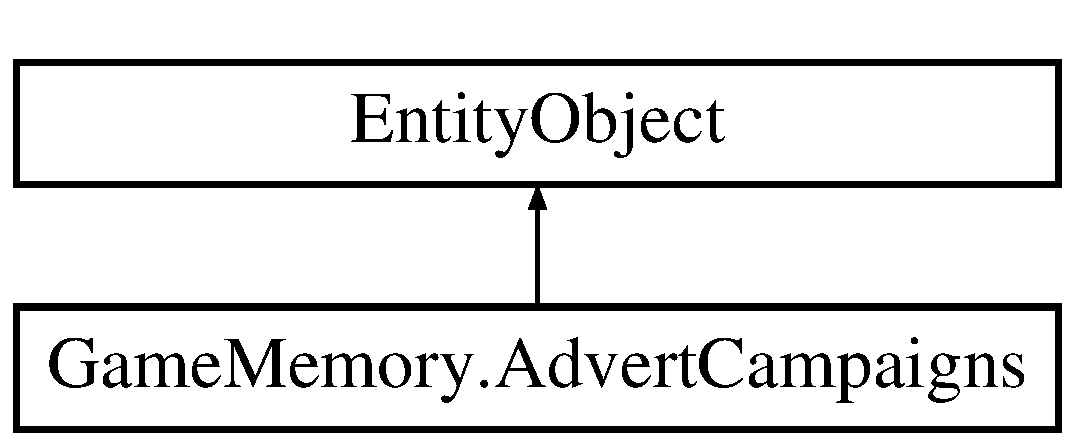
\includegraphics[height=2.000000cm]{class_game_memory_1_1_advert_campaigns}
\end{center}
\end{figure}
\subsection*{Static Public Member Functions}
\begin{DoxyCompactItemize}
\item 
static \hyperlink{class_game_memory_1_1_advert_campaigns}{Advert\-Campaigns} \hyperlink{class_game_memory_1_1_advert_campaigns_af77b777a04e4f249a151540a204d5959}{Create\-Advert\-Campaigns} (global\-::\-System.\-Int32 advert\-Campaign\-Id, global\-::\-System.\-Int32 customer\-Id, global\-::\-System.\-Int32 network\-Id, global\-::\-System.\-Int32 campaign\-Location\-Id, global\-::\-System.\-Int32 campaign\-State\-Id, global\-::\-System.\-Int32 campaign\-Type\-Id)
\begin{DoxyCompactList}\small\item\em Crear un nuevo objeto \hyperlink{class_game_memory_1_1_advert_campaigns}{Advert\-Campaigns}. \end{DoxyCompactList}\end{DoxyCompactItemize}
\subsection*{Properties}
\begin{DoxyCompactItemize}
\item 
global\-::\-System.\-Int32 \hyperlink{class_game_memory_1_1_advert_campaigns_ac2975a0fe8a976df5913d28aad480de8}{Advert\-Campaign\-Id}\hspace{0.3cm}{\ttfamily  \mbox{[}get, set\mbox{]}}
\begin{DoxyCompactList}\small\item\em No hay documentación de metadatos disponible. \end{DoxyCompactList}\item 
global\-::\-System.\-Int32 \hyperlink{class_game_memory_1_1_advert_campaigns_a3bbff19846dd4093f2e35a474d46052f}{Customer\-Id}\hspace{0.3cm}{\ttfamily  \mbox{[}get, set\mbox{]}}
\begin{DoxyCompactList}\small\item\em No hay documentación de metadatos disponible. \end{DoxyCompactList}\item 
global\-::\-System.\-String \hyperlink{class_game_memory_1_1_advert_campaigns_a21f383f075ec3feed11b31fae8b68776}{Name}\hspace{0.3cm}{\ttfamily  \mbox{[}get, set\mbox{]}}
\begin{DoxyCompactList}\small\item\em No hay documentación de metadatos disponible. \end{DoxyCompactList}\item 
global\-::\-System.\-Int32 \hyperlink{class_game_memory_1_1_advert_campaigns_ab1f17469e47f312a306fcb0b971a51d8}{Network\-Id}\hspace{0.3cm}{\ttfamily  \mbox{[}get, set\mbox{]}}
\begin{DoxyCompactList}\small\item\em No hay documentación de metadatos disponible. \end{DoxyCompactList}\item 
global\-::\-System.\-Int32 \hyperlink{class_game_memory_1_1_advert_campaigns_ab079c6a8af8543da827b0ddee5ff574b}{Campaign\-Location\-Id}\hspace{0.3cm}{\ttfamily  \mbox{[}get, set\mbox{]}}
\begin{DoxyCompactList}\small\item\em No hay documentación de metadatos disponible. \end{DoxyCompactList}\item 
Nullable$<$ global\-::\-System.\-Date\-Time $>$ \hyperlink{class_game_memory_1_1_advert_campaigns_a049a795b17f180045f49fabc2d826fe5}{End\-Datetime}\hspace{0.3cm}{\ttfamily  \mbox{[}get, set\mbox{]}}
\begin{DoxyCompactList}\small\item\em No hay documentación de metadatos disponible. \end{DoxyCompactList}\item 
Nullable$<$ global\-::\-System.\-Date\-Time $>$ \hyperlink{class_game_memory_1_1_advert_campaigns_a97c112e92c8edbcc4fa00ed2573de907}{Start\-Datetime}\hspace{0.3cm}{\ttfamily  \mbox{[}get, set\mbox{]}}
\begin{DoxyCompactList}\small\item\em No hay documentación de metadatos disponible. \end{DoxyCompactList}\item 
Nullable$<$ global\-::\-System.\-Date\-Time $>$ \hyperlink{class_game_memory_1_1_advert_campaigns_ac344d89b4ad8fb19599f44c9fa915241}{Last\-Update}\hspace{0.3cm}{\ttfamily  \mbox{[}get, set\mbox{]}}
\begin{DoxyCompactList}\small\item\em No hay documentación de metadatos disponible. \end{DoxyCompactList}\item 
Nullable$<$ global\-::\-System.\-Date\-Time $>$ \hyperlink{class_game_memory_1_1_advert_campaigns_a2a4e8304035a50ff877a6486d60a9e3e}{Created\-Date}\hspace{0.3cm}{\ttfamily  \mbox{[}get, set\mbox{]}}
\begin{DoxyCompactList}\small\item\em No hay documentación de metadatos disponible. \end{DoxyCompactList}\item 
global\-::\-System.\-Int32 \hyperlink{class_game_memory_1_1_advert_campaigns_aaeb4c0190abc0c16f835d17371cb8449}{Campaign\-State\-Id}\hspace{0.3cm}{\ttfamily  \mbox{[}get, set\mbox{]}}
\begin{DoxyCompactList}\small\item\em No hay documentación de metadatos disponible. \end{DoxyCompactList}\item 
global\-::\-System.\-Int32 \hyperlink{class_game_memory_1_1_advert_campaigns_a8ea07608b924d2ab48832ead8bd743a1}{Campaign\-Type\-Id}\hspace{0.3cm}{\ttfamily  \mbox{[}get, set\mbox{]}}
\begin{DoxyCompactList}\small\item\em No hay documentación de metadatos disponible. \end{DoxyCompactList}\item 
Nullable$<$ global\-::\-System.\-Decimal $>$ \hyperlink{class_game_memory_1_1_advert_campaigns_a7522ba2501af95ad0ca28b9ca1e3230a}{Estimate}\hspace{0.3cm}{\ttfamily  \mbox{[}get, set\mbox{]}}
\begin{DoxyCompactList}\small\item\em No hay documentación de metadatos disponible. \end{DoxyCompactList}\item 
Nullable$<$ global\-::\-System.\-Decimal $>$ \hyperlink{class_game_memory_1_1_advert_campaigns_a9d2fcb82eb2b201a608017335a28567e}{Offer}\hspace{0.3cm}{\ttfamily  \mbox{[}get, set\mbox{]}}
\begin{DoxyCompactList}\small\item\em No hay documentación de metadatos disponible. \end{DoxyCompactList}\item 
Entity\-Collection\\*
$<$ \hyperlink{class_game_memory_1_1_advert_campaign_details}{Advert\-Campaign\-Details} $>$ \hyperlink{class_game_memory_1_1_advert_campaigns_a6e7c57f8db8798bdbdddcaafa8e8cbae}{Advert\-Campaign\-Details}\hspace{0.3cm}{\ttfamily  \mbox{[}get, set\mbox{]}}
\begin{DoxyCompactList}\small\item\em No hay documentación de metadatos disponible. \end{DoxyCompactList}\item 
Entity\-Collection\\*
$<$ \hyperlink{class_game_memory_1_1_advert_campaign_interactions}{Advert\-Campaign\-Interactions} $>$ \hyperlink{class_game_memory_1_1_advert_campaigns_af100fbf823e76ee9df9436ac59717435}{Advert\-Campaign\-Interactions}\hspace{0.3cm}{\ttfamily  \mbox{[}get, set\mbox{]}}
\begin{DoxyCompactList}\small\item\em No hay documentación de metadatos disponible. \end{DoxyCompactList}\item 
\hyperlink{class_game_memory_1_1_campaign_locations}{Campaign\-Locations} \hyperlink{class_game_memory_1_1_advert_campaigns_ab28b02102aeef1788ca6e1dd3bb6a098}{Campaign\-Locations}\hspace{0.3cm}{\ttfamily  \mbox{[}get, set\mbox{]}}
\begin{DoxyCompactList}\small\item\em No hay documentación de metadatos disponible. \end{DoxyCompactList}\item 
Entity\-Reference\\*
$<$ \hyperlink{class_game_memory_1_1_campaign_locations}{Campaign\-Locations} $>$ \hyperlink{class_game_memory_1_1_advert_campaigns_a1fbf3e6ceb5391084f9510ca735847de}{Campaign\-Locations\-Reference}\hspace{0.3cm}{\ttfamily  \mbox{[}get, set\mbox{]}}
\begin{DoxyCompactList}\small\item\em No hay documentación de metadatos disponible. \end{DoxyCompactList}\item 
\hyperlink{class_game_memory_1_1_campaign_states}{Campaign\-States} \hyperlink{class_game_memory_1_1_advert_campaigns_ab254e90abef7201a8b4a9cb314df6e1b}{Campaign\-States}\hspace{0.3cm}{\ttfamily  \mbox{[}get, set\mbox{]}}
\begin{DoxyCompactList}\small\item\em No hay documentación de metadatos disponible. \end{DoxyCompactList}\item 
Entity\-Reference$<$ \hyperlink{class_game_memory_1_1_campaign_states}{Campaign\-States} $>$ \hyperlink{class_game_memory_1_1_advert_campaigns_a2b666e7a41a4408e76ca8cb79c99ad7b}{Campaign\-States\-Reference}\hspace{0.3cm}{\ttfamily  \mbox{[}get, set\mbox{]}}
\begin{DoxyCompactList}\small\item\em No hay documentación de metadatos disponible. \end{DoxyCompactList}\item 
\hyperlink{class_game_memory_1_1_campaign_types}{Campaign\-Types} \hyperlink{class_game_memory_1_1_advert_campaigns_a2248329f3b61f4745a02e612e9f597bb}{Campaign\-Types}\hspace{0.3cm}{\ttfamily  \mbox{[}get, set\mbox{]}}
\begin{DoxyCompactList}\small\item\em No hay documentación de metadatos disponible. \end{DoxyCompactList}\item 
Entity\-Reference$<$ \hyperlink{class_game_memory_1_1_campaign_types}{Campaign\-Types} $>$ \hyperlink{class_game_memory_1_1_advert_campaigns_ade5c3b4524c9c97b3ecd4e584839217c}{Campaign\-Types\-Reference}\hspace{0.3cm}{\ttfamily  \mbox{[}get, set\mbox{]}}
\begin{DoxyCompactList}\small\item\em No hay documentación de metadatos disponible. \end{DoxyCompactList}\item 
\hyperlink{class_game_memory_1_1_customers}{Customers} \hyperlink{class_game_memory_1_1_advert_campaigns_aa63acf86fef731a20b8d1b4b6842fa54}{Customers}\hspace{0.3cm}{\ttfamily  \mbox{[}get, set\mbox{]}}
\begin{DoxyCompactList}\small\item\em No hay documentación de metadatos disponible. \end{DoxyCompactList}\item 
Entity\-Reference$<$ \hyperlink{class_game_memory_1_1_customers}{Customers} $>$ \hyperlink{class_game_memory_1_1_advert_campaigns_a3a0f33054dc2f41e592a3504783abfa8}{Customers\-Reference}\hspace{0.3cm}{\ttfamily  \mbox{[}get, set\mbox{]}}
\begin{DoxyCompactList}\small\item\em No hay documentación de metadatos disponible. \end{DoxyCompactList}\item 
\hyperlink{class_game_memory_1_1_networks}{Networks} \hyperlink{class_game_memory_1_1_advert_campaigns_a93fb9fb1604fb97b196e6cd7186270cf}{Networks}\hspace{0.3cm}{\ttfamily  \mbox{[}get, set\mbox{]}}
\begin{DoxyCompactList}\small\item\em No hay documentación de metadatos disponible. \end{DoxyCompactList}\item 
Entity\-Reference$<$ \hyperlink{class_game_memory_1_1_networks}{Networks} $>$ \hyperlink{class_game_memory_1_1_advert_campaigns_a31ed9dd24ca6e2155bc0f19a55053e63}{Networks\-Reference}\hspace{0.3cm}{\ttfamily  \mbox{[}get, set\mbox{]}}
\begin{DoxyCompactList}\small\item\em No hay documentación de metadatos disponible. \end{DoxyCompactList}\item 
Entity\-Collection$<$ \hyperlink{class_game_memory_1_1_advert_hosts}{Advert\-Hosts} $>$ \hyperlink{class_game_memory_1_1_advert_campaigns_a448c21e840bad8b62dbda780cb093f0e}{Advert\-Hosts}\hspace{0.3cm}{\ttfamily  \mbox{[}get, set\mbox{]}}
\begin{DoxyCompactList}\small\item\em No hay documentación de metadatos disponible. \end{DoxyCompactList}\end{DoxyCompactItemize}


\subsection{Detailed Description}
No hay documentación de metadatos disponible. 



\subsection{Member Function Documentation}
\hypertarget{class_game_memory_1_1_advert_campaigns_af77b777a04e4f249a151540a204d5959}{\index{Game\-Memory\-::\-Advert\-Campaigns@{Game\-Memory\-::\-Advert\-Campaigns}!Create\-Advert\-Campaigns@{Create\-Advert\-Campaigns}}
\index{Create\-Advert\-Campaigns@{Create\-Advert\-Campaigns}!GameMemory::AdvertCampaigns@{Game\-Memory\-::\-Advert\-Campaigns}}
\subsubsection[{Create\-Advert\-Campaigns}]{\setlength{\rightskip}{0pt plus 5cm}static {\bf Advert\-Campaigns} Game\-Memory.\-Advert\-Campaigns.\-Create\-Advert\-Campaigns (
\begin{DoxyParamCaption}
\item[{global\-::\-System.\-Int32}]{advert\-Campaign\-Id, }
\item[{global\-::\-System.\-Int32}]{customer\-Id, }
\item[{global\-::\-System.\-Int32}]{network\-Id, }
\item[{global\-::\-System.\-Int32}]{campaign\-Location\-Id, }
\item[{global\-::\-System.\-Int32}]{campaign\-State\-Id, }
\item[{global\-::\-System.\-Int32}]{campaign\-Type\-Id}
\end{DoxyParamCaption}
)\hspace{0.3cm}{\ttfamily [static]}}}\label{class_game_memory_1_1_advert_campaigns_af77b777a04e4f249a151540a204d5959}


Crear un nuevo objeto \hyperlink{class_game_memory_1_1_advert_campaigns}{Advert\-Campaigns}. 


\begin{DoxyParams}{Parameters}
{\em advert\-Campaign\-Id} & Valor inicial de la propiedad Advert\-Campaign\-Id.\\
\hline
{\em customer\-Id} & Valor inicial de la propiedad Customer\-Id.\\
\hline
{\em network\-Id} & Valor inicial de la propiedad Network\-Id.\\
\hline
{\em campaign\-Location\-Id} & Valor inicial de la propiedad Campaign\-Location\-Id.\\
\hline
{\em campaign\-State\-Id} & Valor inicial de la propiedad Campaign\-State\-Id.\\
\hline
{\em campaign\-Type\-Id} & Valor inicial de la propiedad Campaign\-Type\-Id.\\
\hline
\end{DoxyParams}


\subsection{Property Documentation}
\hypertarget{class_game_memory_1_1_advert_campaigns_a6e7c57f8db8798bdbdddcaafa8e8cbae}{\index{Game\-Memory\-::\-Advert\-Campaigns@{Game\-Memory\-::\-Advert\-Campaigns}!Advert\-Campaign\-Details@{Advert\-Campaign\-Details}}
\index{Advert\-Campaign\-Details@{Advert\-Campaign\-Details}!GameMemory::AdvertCampaigns@{Game\-Memory\-::\-Advert\-Campaigns}}
\subsubsection[{Advert\-Campaign\-Details}]{\setlength{\rightskip}{0pt plus 5cm}Entity\-Collection$<${\bf Advert\-Campaign\-Details}$>$ Game\-Memory.\-Advert\-Campaigns.\-Advert\-Campaign\-Details\hspace{0.3cm}{\ttfamily [get]}, {\ttfamily [set]}}}\label{class_game_memory_1_1_advert_campaigns_a6e7c57f8db8798bdbdddcaafa8e8cbae}


No hay documentación de metadatos disponible. 

\hypertarget{class_game_memory_1_1_advert_campaigns_ac2975a0fe8a976df5913d28aad480de8}{\index{Game\-Memory\-::\-Advert\-Campaigns@{Game\-Memory\-::\-Advert\-Campaigns}!Advert\-Campaign\-Id@{Advert\-Campaign\-Id}}
\index{Advert\-Campaign\-Id@{Advert\-Campaign\-Id}!GameMemory::AdvertCampaigns@{Game\-Memory\-::\-Advert\-Campaigns}}
\subsubsection[{Advert\-Campaign\-Id}]{\setlength{\rightskip}{0pt plus 5cm}global.\-System.\-Int32 Game\-Memory.\-Advert\-Campaigns.\-Advert\-Campaign\-Id\hspace{0.3cm}{\ttfamily [get]}, {\ttfamily [set]}}}\label{class_game_memory_1_1_advert_campaigns_ac2975a0fe8a976df5913d28aad480de8}


No hay documentación de metadatos disponible. 

\hypertarget{class_game_memory_1_1_advert_campaigns_af100fbf823e76ee9df9436ac59717435}{\index{Game\-Memory\-::\-Advert\-Campaigns@{Game\-Memory\-::\-Advert\-Campaigns}!Advert\-Campaign\-Interactions@{Advert\-Campaign\-Interactions}}
\index{Advert\-Campaign\-Interactions@{Advert\-Campaign\-Interactions}!GameMemory::AdvertCampaigns@{Game\-Memory\-::\-Advert\-Campaigns}}
\subsubsection[{Advert\-Campaign\-Interactions}]{\setlength{\rightskip}{0pt plus 5cm}Entity\-Collection$<${\bf Advert\-Campaign\-Interactions}$>$ Game\-Memory.\-Advert\-Campaigns.\-Advert\-Campaign\-Interactions\hspace{0.3cm}{\ttfamily [get]}, {\ttfamily [set]}}}\label{class_game_memory_1_1_advert_campaigns_af100fbf823e76ee9df9436ac59717435}


No hay documentación de metadatos disponible. 

\hypertarget{class_game_memory_1_1_advert_campaigns_a448c21e840bad8b62dbda780cb093f0e}{\index{Game\-Memory\-::\-Advert\-Campaigns@{Game\-Memory\-::\-Advert\-Campaigns}!Advert\-Hosts@{Advert\-Hosts}}
\index{Advert\-Hosts@{Advert\-Hosts}!GameMemory::AdvertCampaigns@{Game\-Memory\-::\-Advert\-Campaigns}}
\subsubsection[{Advert\-Hosts}]{\setlength{\rightskip}{0pt plus 5cm}Entity\-Collection$<${\bf Advert\-Hosts}$>$ Game\-Memory.\-Advert\-Campaigns.\-Advert\-Hosts\hspace{0.3cm}{\ttfamily [get]}, {\ttfamily [set]}}}\label{class_game_memory_1_1_advert_campaigns_a448c21e840bad8b62dbda780cb093f0e}


No hay documentación de metadatos disponible. 

\hypertarget{class_game_memory_1_1_advert_campaigns_ab079c6a8af8543da827b0ddee5ff574b}{\index{Game\-Memory\-::\-Advert\-Campaigns@{Game\-Memory\-::\-Advert\-Campaigns}!Campaign\-Location\-Id@{Campaign\-Location\-Id}}
\index{Campaign\-Location\-Id@{Campaign\-Location\-Id}!GameMemory::AdvertCampaigns@{Game\-Memory\-::\-Advert\-Campaigns}}
\subsubsection[{Campaign\-Location\-Id}]{\setlength{\rightskip}{0pt plus 5cm}global.\-System.\-Int32 Game\-Memory.\-Advert\-Campaigns.\-Campaign\-Location\-Id\hspace{0.3cm}{\ttfamily [get]}, {\ttfamily [set]}}}\label{class_game_memory_1_1_advert_campaigns_ab079c6a8af8543da827b0ddee5ff574b}


No hay documentación de metadatos disponible. 

\hypertarget{class_game_memory_1_1_advert_campaigns_ab28b02102aeef1788ca6e1dd3bb6a098}{\index{Game\-Memory\-::\-Advert\-Campaigns@{Game\-Memory\-::\-Advert\-Campaigns}!Campaign\-Locations@{Campaign\-Locations}}
\index{Campaign\-Locations@{Campaign\-Locations}!GameMemory::AdvertCampaigns@{Game\-Memory\-::\-Advert\-Campaigns}}
\subsubsection[{Campaign\-Locations}]{\setlength{\rightskip}{0pt plus 5cm}{\bf Campaign\-Locations} Game\-Memory.\-Advert\-Campaigns.\-Campaign\-Locations\hspace{0.3cm}{\ttfamily [get]}, {\ttfamily [set]}}}\label{class_game_memory_1_1_advert_campaigns_ab28b02102aeef1788ca6e1dd3bb6a098}


No hay documentación de metadatos disponible. 

\hypertarget{class_game_memory_1_1_advert_campaigns_a1fbf3e6ceb5391084f9510ca735847de}{\index{Game\-Memory\-::\-Advert\-Campaigns@{Game\-Memory\-::\-Advert\-Campaigns}!Campaign\-Locations\-Reference@{Campaign\-Locations\-Reference}}
\index{Campaign\-Locations\-Reference@{Campaign\-Locations\-Reference}!GameMemory::AdvertCampaigns@{Game\-Memory\-::\-Advert\-Campaigns}}
\subsubsection[{Campaign\-Locations\-Reference}]{\setlength{\rightskip}{0pt plus 5cm}Entity\-Reference$<${\bf Campaign\-Locations}$>$ Game\-Memory.\-Advert\-Campaigns.\-Campaign\-Locations\-Reference\hspace{0.3cm}{\ttfamily [get]}, {\ttfamily [set]}}}\label{class_game_memory_1_1_advert_campaigns_a1fbf3e6ceb5391084f9510ca735847de}


No hay documentación de metadatos disponible. 

\hypertarget{class_game_memory_1_1_advert_campaigns_aaeb4c0190abc0c16f835d17371cb8449}{\index{Game\-Memory\-::\-Advert\-Campaigns@{Game\-Memory\-::\-Advert\-Campaigns}!Campaign\-State\-Id@{Campaign\-State\-Id}}
\index{Campaign\-State\-Id@{Campaign\-State\-Id}!GameMemory::AdvertCampaigns@{Game\-Memory\-::\-Advert\-Campaigns}}
\subsubsection[{Campaign\-State\-Id}]{\setlength{\rightskip}{0pt plus 5cm}global.\-System.\-Int32 Game\-Memory.\-Advert\-Campaigns.\-Campaign\-State\-Id\hspace{0.3cm}{\ttfamily [get]}, {\ttfamily [set]}}}\label{class_game_memory_1_1_advert_campaigns_aaeb4c0190abc0c16f835d17371cb8449}


No hay documentación de metadatos disponible. 

\hypertarget{class_game_memory_1_1_advert_campaigns_ab254e90abef7201a8b4a9cb314df6e1b}{\index{Game\-Memory\-::\-Advert\-Campaigns@{Game\-Memory\-::\-Advert\-Campaigns}!Campaign\-States@{Campaign\-States}}
\index{Campaign\-States@{Campaign\-States}!GameMemory::AdvertCampaigns@{Game\-Memory\-::\-Advert\-Campaigns}}
\subsubsection[{Campaign\-States}]{\setlength{\rightskip}{0pt plus 5cm}{\bf Campaign\-States} Game\-Memory.\-Advert\-Campaigns.\-Campaign\-States\hspace{0.3cm}{\ttfamily [get]}, {\ttfamily [set]}}}\label{class_game_memory_1_1_advert_campaigns_ab254e90abef7201a8b4a9cb314df6e1b}


No hay documentación de metadatos disponible. 

\hypertarget{class_game_memory_1_1_advert_campaigns_a2b666e7a41a4408e76ca8cb79c99ad7b}{\index{Game\-Memory\-::\-Advert\-Campaigns@{Game\-Memory\-::\-Advert\-Campaigns}!Campaign\-States\-Reference@{Campaign\-States\-Reference}}
\index{Campaign\-States\-Reference@{Campaign\-States\-Reference}!GameMemory::AdvertCampaigns@{Game\-Memory\-::\-Advert\-Campaigns}}
\subsubsection[{Campaign\-States\-Reference}]{\setlength{\rightskip}{0pt plus 5cm}Entity\-Reference$<${\bf Campaign\-States}$>$ Game\-Memory.\-Advert\-Campaigns.\-Campaign\-States\-Reference\hspace{0.3cm}{\ttfamily [get]}, {\ttfamily [set]}}}\label{class_game_memory_1_1_advert_campaigns_a2b666e7a41a4408e76ca8cb79c99ad7b}


No hay documentación de metadatos disponible. 

\hypertarget{class_game_memory_1_1_advert_campaigns_a8ea07608b924d2ab48832ead8bd743a1}{\index{Game\-Memory\-::\-Advert\-Campaigns@{Game\-Memory\-::\-Advert\-Campaigns}!Campaign\-Type\-Id@{Campaign\-Type\-Id}}
\index{Campaign\-Type\-Id@{Campaign\-Type\-Id}!GameMemory::AdvertCampaigns@{Game\-Memory\-::\-Advert\-Campaigns}}
\subsubsection[{Campaign\-Type\-Id}]{\setlength{\rightskip}{0pt plus 5cm}global.\-System.\-Int32 Game\-Memory.\-Advert\-Campaigns.\-Campaign\-Type\-Id\hspace{0.3cm}{\ttfamily [get]}, {\ttfamily [set]}}}\label{class_game_memory_1_1_advert_campaigns_a8ea07608b924d2ab48832ead8bd743a1}


No hay documentación de metadatos disponible. 

\hypertarget{class_game_memory_1_1_advert_campaigns_a2248329f3b61f4745a02e612e9f597bb}{\index{Game\-Memory\-::\-Advert\-Campaigns@{Game\-Memory\-::\-Advert\-Campaigns}!Campaign\-Types@{Campaign\-Types}}
\index{Campaign\-Types@{Campaign\-Types}!GameMemory::AdvertCampaigns@{Game\-Memory\-::\-Advert\-Campaigns}}
\subsubsection[{Campaign\-Types}]{\setlength{\rightskip}{0pt plus 5cm}{\bf Campaign\-Types} Game\-Memory.\-Advert\-Campaigns.\-Campaign\-Types\hspace{0.3cm}{\ttfamily [get]}, {\ttfamily [set]}}}\label{class_game_memory_1_1_advert_campaigns_a2248329f3b61f4745a02e612e9f597bb}


No hay documentación de metadatos disponible. 

\hypertarget{class_game_memory_1_1_advert_campaigns_ade5c3b4524c9c97b3ecd4e584839217c}{\index{Game\-Memory\-::\-Advert\-Campaigns@{Game\-Memory\-::\-Advert\-Campaigns}!Campaign\-Types\-Reference@{Campaign\-Types\-Reference}}
\index{Campaign\-Types\-Reference@{Campaign\-Types\-Reference}!GameMemory::AdvertCampaigns@{Game\-Memory\-::\-Advert\-Campaigns}}
\subsubsection[{Campaign\-Types\-Reference}]{\setlength{\rightskip}{0pt plus 5cm}Entity\-Reference$<${\bf Campaign\-Types}$>$ Game\-Memory.\-Advert\-Campaigns.\-Campaign\-Types\-Reference\hspace{0.3cm}{\ttfamily [get]}, {\ttfamily [set]}}}\label{class_game_memory_1_1_advert_campaigns_ade5c3b4524c9c97b3ecd4e584839217c}


No hay documentación de metadatos disponible. 

\hypertarget{class_game_memory_1_1_advert_campaigns_a2a4e8304035a50ff877a6486d60a9e3e}{\index{Game\-Memory\-::\-Advert\-Campaigns@{Game\-Memory\-::\-Advert\-Campaigns}!Created\-Date@{Created\-Date}}
\index{Created\-Date@{Created\-Date}!GameMemory::AdvertCampaigns@{Game\-Memory\-::\-Advert\-Campaigns}}
\subsubsection[{Created\-Date}]{\setlength{\rightskip}{0pt plus 5cm}Nullable$<$global.\-System.\-Date\-Time$>$ Game\-Memory.\-Advert\-Campaigns.\-Created\-Date\hspace{0.3cm}{\ttfamily [get]}, {\ttfamily [set]}}}\label{class_game_memory_1_1_advert_campaigns_a2a4e8304035a50ff877a6486d60a9e3e}


No hay documentación de metadatos disponible. 

\hypertarget{class_game_memory_1_1_advert_campaigns_a3bbff19846dd4093f2e35a474d46052f}{\index{Game\-Memory\-::\-Advert\-Campaigns@{Game\-Memory\-::\-Advert\-Campaigns}!Customer\-Id@{Customer\-Id}}
\index{Customer\-Id@{Customer\-Id}!GameMemory::AdvertCampaigns@{Game\-Memory\-::\-Advert\-Campaigns}}
\subsubsection[{Customer\-Id}]{\setlength{\rightskip}{0pt plus 5cm}global.\-System.\-Int32 Game\-Memory.\-Advert\-Campaigns.\-Customer\-Id\hspace{0.3cm}{\ttfamily [get]}, {\ttfamily [set]}}}\label{class_game_memory_1_1_advert_campaigns_a3bbff19846dd4093f2e35a474d46052f}


No hay documentación de metadatos disponible. 

\hypertarget{class_game_memory_1_1_advert_campaigns_aa63acf86fef731a20b8d1b4b6842fa54}{\index{Game\-Memory\-::\-Advert\-Campaigns@{Game\-Memory\-::\-Advert\-Campaigns}!Customers@{Customers}}
\index{Customers@{Customers}!GameMemory::AdvertCampaigns@{Game\-Memory\-::\-Advert\-Campaigns}}
\subsubsection[{Customers}]{\setlength{\rightskip}{0pt plus 5cm}{\bf Customers} Game\-Memory.\-Advert\-Campaigns.\-Customers\hspace{0.3cm}{\ttfamily [get]}, {\ttfamily [set]}}}\label{class_game_memory_1_1_advert_campaigns_aa63acf86fef731a20b8d1b4b6842fa54}


No hay documentación de metadatos disponible. 

\hypertarget{class_game_memory_1_1_advert_campaigns_a3a0f33054dc2f41e592a3504783abfa8}{\index{Game\-Memory\-::\-Advert\-Campaigns@{Game\-Memory\-::\-Advert\-Campaigns}!Customers\-Reference@{Customers\-Reference}}
\index{Customers\-Reference@{Customers\-Reference}!GameMemory::AdvertCampaigns@{Game\-Memory\-::\-Advert\-Campaigns}}
\subsubsection[{Customers\-Reference}]{\setlength{\rightskip}{0pt plus 5cm}Entity\-Reference$<${\bf Customers}$>$ Game\-Memory.\-Advert\-Campaigns.\-Customers\-Reference\hspace{0.3cm}{\ttfamily [get]}, {\ttfamily [set]}}}\label{class_game_memory_1_1_advert_campaigns_a3a0f33054dc2f41e592a3504783abfa8}


No hay documentación de metadatos disponible. 

\hypertarget{class_game_memory_1_1_advert_campaigns_a049a795b17f180045f49fabc2d826fe5}{\index{Game\-Memory\-::\-Advert\-Campaigns@{Game\-Memory\-::\-Advert\-Campaigns}!End\-Datetime@{End\-Datetime}}
\index{End\-Datetime@{End\-Datetime}!GameMemory::AdvertCampaigns@{Game\-Memory\-::\-Advert\-Campaigns}}
\subsubsection[{End\-Datetime}]{\setlength{\rightskip}{0pt plus 5cm}Nullable$<$global.\-System.\-Date\-Time$>$ Game\-Memory.\-Advert\-Campaigns.\-End\-Datetime\hspace{0.3cm}{\ttfamily [get]}, {\ttfamily [set]}}}\label{class_game_memory_1_1_advert_campaigns_a049a795b17f180045f49fabc2d826fe5}


No hay documentación de metadatos disponible. 

\hypertarget{class_game_memory_1_1_advert_campaigns_a7522ba2501af95ad0ca28b9ca1e3230a}{\index{Game\-Memory\-::\-Advert\-Campaigns@{Game\-Memory\-::\-Advert\-Campaigns}!Estimate@{Estimate}}
\index{Estimate@{Estimate}!GameMemory::AdvertCampaigns@{Game\-Memory\-::\-Advert\-Campaigns}}
\subsubsection[{Estimate}]{\setlength{\rightskip}{0pt plus 5cm}Nullable$<$global.\-System.\-Decimal$>$ Game\-Memory.\-Advert\-Campaigns.\-Estimate\hspace{0.3cm}{\ttfamily [get]}, {\ttfamily [set]}}}\label{class_game_memory_1_1_advert_campaigns_a7522ba2501af95ad0ca28b9ca1e3230a}


No hay documentación de metadatos disponible. 

\hypertarget{class_game_memory_1_1_advert_campaigns_ac344d89b4ad8fb19599f44c9fa915241}{\index{Game\-Memory\-::\-Advert\-Campaigns@{Game\-Memory\-::\-Advert\-Campaigns}!Last\-Update@{Last\-Update}}
\index{Last\-Update@{Last\-Update}!GameMemory::AdvertCampaigns@{Game\-Memory\-::\-Advert\-Campaigns}}
\subsubsection[{Last\-Update}]{\setlength{\rightskip}{0pt plus 5cm}Nullable$<$global.\-System.\-Date\-Time$>$ Game\-Memory.\-Advert\-Campaigns.\-Last\-Update\hspace{0.3cm}{\ttfamily [get]}, {\ttfamily [set]}}}\label{class_game_memory_1_1_advert_campaigns_ac344d89b4ad8fb19599f44c9fa915241}


No hay documentación de metadatos disponible. 

\hypertarget{class_game_memory_1_1_advert_campaigns_a21f383f075ec3feed11b31fae8b68776}{\index{Game\-Memory\-::\-Advert\-Campaigns@{Game\-Memory\-::\-Advert\-Campaigns}!Name@{Name}}
\index{Name@{Name}!GameMemory::AdvertCampaigns@{Game\-Memory\-::\-Advert\-Campaigns}}
\subsubsection[{Name}]{\setlength{\rightskip}{0pt plus 5cm}global.\-System.\-String Game\-Memory.\-Advert\-Campaigns.\-Name\hspace{0.3cm}{\ttfamily [get]}, {\ttfamily [set]}}}\label{class_game_memory_1_1_advert_campaigns_a21f383f075ec3feed11b31fae8b68776}


No hay documentación de metadatos disponible. 

\hypertarget{class_game_memory_1_1_advert_campaigns_ab1f17469e47f312a306fcb0b971a51d8}{\index{Game\-Memory\-::\-Advert\-Campaigns@{Game\-Memory\-::\-Advert\-Campaigns}!Network\-Id@{Network\-Id}}
\index{Network\-Id@{Network\-Id}!GameMemory::AdvertCampaigns@{Game\-Memory\-::\-Advert\-Campaigns}}
\subsubsection[{Network\-Id}]{\setlength{\rightskip}{0pt plus 5cm}global.\-System.\-Int32 Game\-Memory.\-Advert\-Campaigns.\-Network\-Id\hspace{0.3cm}{\ttfamily [get]}, {\ttfamily [set]}}}\label{class_game_memory_1_1_advert_campaigns_ab1f17469e47f312a306fcb0b971a51d8}


No hay documentación de metadatos disponible. 

\hypertarget{class_game_memory_1_1_advert_campaigns_a93fb9fb1604fb97b196e6cd7186270cf}{\index{Game\-Memory\-::\-Advert\-Campaigns@{Game\-Memory\-::\-Advert\-Campaigns}!Networks@{Networks}}
\index{Networks@{Networks}!GameMemory::AdvertCampaigns@{Game\-Memory\-::\-Advert\-Campaigns}}
\subsubsection[{Networks}]{\setlength{\rightskip}{0pt plus 5cm}{\bf Networks} Game\-Memory.\-Advert\-Campaigns.\-Networks\hspace{0.3cm}{\ttfamily [get]}, {\ttfamily [set]}}}\label{class_game_memory_1_1_advert_campaigns_a93fb9fb1604fb97b196e6cd7186270cf}


No hay documentación de metadatos disponible. 

\hypertarget{class_game_memory_1_1_advert_campaigns_a31ed9dd24ca6e2155bc0f19a55053e63}{\index{Game\-Memory\-::\-Advert\-Campaigns@{Game\-Memory\-::\-Advert\-Campaigns}!Networks\-Reference@{Networks\-Reference}}
\index{Networks\-Reference@{Networks\-Reference}!GameMemory::AdvertCampaigns@{Game\-Memory\-::\-Advert\-Campaigns}}
\subsubsection[{Networks\-Reference}]{\setlength{\rightskip}{0pt plus 5cm}Entity\-Reference$<${\bf Networks}$>$ Game\-Memory.\-Advert\-Campaigns.\-Networks\-Reference\hspace{0.3cm}{\ttfamily [get]}, {\ttfamily [set]}}}\label{class_game_memory_1_1_advert_campaigns_a31ed9dd24ca6e2155bc0f19a55053e63}


No hay documentación de metadatos disponible. 

\hypertarget{class_game_memory_1_1_advert_campaigns_a9d2fcb82eb2b201a608017335a28567e}{\index{Game\-Memory\-::\-Advert\-Campaigns@{Game\-Memory\-::\-Advert\-Campaigns}!Offer@{Offer}}
\index{Offer@{Offer}!GameMemory::AdvertCampaigns@{Game\-Memory\-::\-Advert\-Campaigns}}
\subsubsection[{Offer}]{\setlength{\rightskip}{0pt plus 5cm}Nullable$<$global.\-System.\-Decimal$>$ Game\-Memory.\-Advert\-Campaigns.\-Offer\hspace{0.3cm}{\ttfamily [get]}, {\ttfamily [set]}}}\label{class_game_memory_1_1_advert_campaigns_a9d2fcb82eb2b201a608017335a28567e}


No hay documentación de metadatos disponible. 

\hypertarget{class_game_memory_1_1_advert_campaigns_a97c112e92c8edbcc4fa00ed2573de907}{\index{Game\-Memory\-::\-Advert\-Campaigns@{Game\-Memory\-::\-Advert\-Campaigns}!Start\-Datetime@{Start\-Datetime}}
\index{Start\-Datetime@{Start\-Datetime}!GameMemory::AdvertCampaigns@{Game\-Memory\-::\-Advert\-Campaigns}}
\subsubsection[{Start\-Datetime}]{\setlength{\rightskip}{0pt plus 5cm}Nullable$<$global.\-System.\-Date\-Time$>$ Game\-Memory.\-Advert\-Campaigns.\-Start\-Datetime\hspace{0.3cm}{\ttfamily [get]}, {\ttfamily [set]}}}\label{class_game_memory_1_1_advert_campaigns_a97c112e92c8edbcc4fa00ed2573de907}


No hay documentación de metadatos disponible. 



The documentation for this class was generated from the following file\-:\begin{DoxyCompactItemize}
\item 
D\-:/tesis\-Assembla/branches/\-Branch\-\_\-\-Tesis\-\_\-\-Sprint01/\-Dev/\-Interaction Module/\-Game\-Memory/\-Game\-Memory/O\-M\-K\-T.\-Designer.\-cs\end{DoxyCompactItemize}

\hypertarget{class_game_memory_1_1_advert_host_categories}{\section{Game\-Memory.\-Advert\-Host\-Categories Class Reference}
\label{class_game_memory_1_1_advert_host_categories}\index{Game\-Memory.\-Advert\-Host\-Categories@{Game\-Memory.\-Advert\-Host\-Categories}}
}


No hay documentación de metadatos disponible.  


Inheritance diagram for Game\-Memory.\-Advert\-Host\-Categories\-:\begin{figure}[H]
\begin{center}
\leavevmode
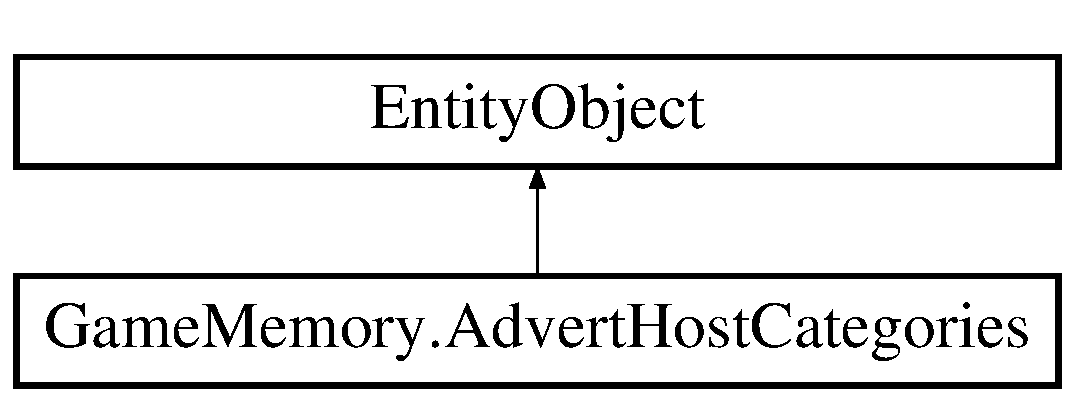
\includegraphics[height=2.000000cm]{class_game_memory_1_1_advert_host_categories}
\end{center}
\end{figure}
\subsection*{Static Public Member Functions}
\begin{DoxyCompactItemize}
\item 
static \hyperlink{class_game_memory_1_1_advert_host_categories}{Advert\-Host\-Categories} \hyperlink{class_game_memory_1_1_advert_host_categories_a1b8c6959d44391b88a93f426c94714d1}{Create\-Advert\-Host\-Categories} (global\-::\-System.\-Int32 advert\-Host\-Category\-Id)
\begin{DoxyCompactList}\small\item\em Crear un nuevo objeto \hyperlink{class_game_memory_1_1_advert_host_categories}{Advert\-Host\-Categories}. \end{DoxyCompactList}\end{DoxyCompactItemize}
\subsection*{Properties}
\begin{DoxyCompactItemize}
\item 
global\-::\-System.\-Int32 \hyperlink{class_game_memory_1_1_advert_host_categories_a8e29b02e2d791d91f54adba5fbbbb015}{Advert\-Host\-Category\-Id}\hspace{0.3cm}{\ttfamily  \mbox{[}get, set\mbox{]}}
\begin{DoxyCompactList}\small\item\em No hay documentación de metadatos disponible. \end{DoxyCompactList}\item 
global\-::\-System.\-String \hyperlink{class_game_memory_1_1_advert_host_categories_a27c87fd89b900401aa077659f344f87f}{Name}\hspace{0.3cm}{\ttfamily  \mbox{[}get, set\mbox{]}}
\begin{DoxyCompactList}\small\item\em No hay documentación de metadatos disponible. \end{DoxyCompactList}\item 
global\-::\-System.\-String \hyperlink{class_game_memory_1_1_advert_host_categories_a192d719edeeeb2188e5f05b036b56de6}{Detail}\hspace{0.3cm}{\ttfamily  \mbox{[}get, set\mbox{]}}
\begin{DoxyCompactList}\small\item\em No hay documentación de metadatos disponible. \end{DoxyCompactList}\item 
Entity\-Collection$<$ \hyperlink{class_game_memory_1_1_advert_hosts}{Advert\-Hosts} $>$ \hyperlink{class_game_memory_1_1_advert_host_categories_a3d8f8d6f01ed2c43921957b1de473fe8}{Advert\-Hosts}\hspace{0.3cm}{\ttfamily  \mbox{[}get, set\mbox{]}}
\begin{DoxyCompactList}\small\item\em No hay documentación de metadatos disponible. \end{DoxyCompactList}\end{DoxyCompactItemize}


\subsection{Detailed Description}
No hay documentación de metadatos disponible. 



\subsection{Member Function Documentation}
\hypertarget{class_game_memory_1_1_advert_host_categories_a1b8c6959d44391b88a93f426c94714d1}{\index{Game\-Memory\-::\-Advert\-Host\-Categories@{Game\-Memory\-::\-Advert\-Host\-Categories}!Create\-Advert\-Host\-Categories@{Create\-Advert\-Host\-Categories}}
\index{Create\-Advert\-Host\-Categories@{Create\-Advert\-Host\-Categories}!GameMemory::AdvertHostCategories@{Game\-Memory\-::\-Advert\-Host\-Categories}}
\subsubsection[{Create\-Advert\-Host\-Categories}]{\setlength{\rightskip}{0pt plus 5cm}static {\bf Advert\-Host\-Categories} Game\-Memory.\-Advert\-Host\-Categories.\-Create\-Advert\-Host\-Categories (
\begin{DoxyParamCaption}
\item[{global\-::\-System.\-Int32}]{advert\-Host\-Category\-Id}
\end{DoxyParamCaption}
)\hspace{0.3cm}{\ttfamily [static]}}}\label{class_game_memory_1_1_advert_host_categories_a1b8c6959d44391b88a93f426c94714d1}


Crear un nuevo objeto \hyperlink{class_game_memory_1_1_advert_host_categories}{Advert\-Host\-Categories}. 


\begin{DoxyParams}{Parameters}
{\em advert\-Host\-Category\-Id} & Valor inicial de la propiedad Advert\-Host\-Category\-Id.\\
\hline
\end{DoxyParams}


\subsection{Property Documentation}
\hypertarget{class_game_memory_1_1_advert_host_categories_a8e29b02e2d791d91f54adba5fbbbb015}{\index{Game\-Memory\-::\-Advert\-Host\-Categories@{Game\-Memory\-::\-Advert\-Host\-Categories}!Advert\-Host\-Category\-Id@{Advert\-Host\-Category\-Id}}
\index{Advert\-Host\-Category\-Id@{Advert\-Host\-Category\-Id}!GameMemory::AdvertHostCategories@{Game\-Memory\-::\-Advert\-Host\-Categories}}
\subsubsection[{Advert\-Host\-Category\-Id}]{\setlength{\rightskip}{0pt plus 5cm}global.\-System.\-Int32 Game\-Memory.\-Advert\-Host\-Categories.\-Advert\-Host\-Category\-Id\hspace{0.3cm}{\ttfamily [get]}, {\ttfamily [set]}}}\label{class_game_memory_1_1_advert_host_categories_a8e29b02e2d791d91f54adba5fbbbb015}


No hay documentación de metadatos disponible. 

\hypertarget{class_game_memory_1_1_advert_host_categories_a3d8f8d6f01ed2c43921957b1de473fe8}{\index{Game\-Memory\-::\-Advert\-Host\-Categories@{Game\-Memory\-::\-Advert\-Host\-Categories}!Advert\-Hosts@{Advert\-Hosts}}
\index{Advert\-Hosts@{Advert\-Hosts}!GameMemory::AdvertHostCategories@{Game\-Memory\-::\-Advert\-Host\-Categories}}
\subsubsection[{Advert\-Hosts}]{\setlength{\rightskip}{0pt plus 5cm}Entity\-Collection$<${\bf Advert\-Hosts}$>$ Game\-Memory.\-Advert\-Host\-Categories.\-Advert\-Hosts\hspace{0.3cm}{\ttfamily [get]}, {\ttfamily [set]}}}\label{class_game_memory_1_1_advert_host_categories_a3d8f8d6f01ed2c43921957b1de473fe8}


No hay documentación de metadatos disponible. 

\hypertarget{class_game_memory_1_1_advert_host_categories_a192d719edeeeb2188e5f05b036b56de6}{\index{Game\-Memory\-::\-Advert\-Host\-Categories@{Game\-Memory\-::\-Advert\-Host\-Categories}!Detail@{Detail}}
\index{Detail@{Detail}!GameMemory::AdvertHostCategories@{Game\-Memory\-::\-Advert\-Host\-Categories}}
\subsubsection[{Detail}]{\setlength{\rightskip}{0pt plus 5cm}global.\-System.\-String Game\-Memory.\-Advert\-Host\-Categories.\-Detail\hspace{0.3cm}{\ttfamily [get]}, {\ttfamily [set]}}}\label{class_game_memory_1_1_advert_host_categories_a192d719edeeeb2188e5f05b036b56de6}


No hay documentación de metadatos disponible. 

\hypertarget{class_game_memory_1_1_advert_host_categories_a27c87fd89b900401aa077659f344f87f}{\index{Game\-Memory\-::\-Advert\-Host\-Categories@{Game\-Memory\-::\-Advert\-Host\-Categories}!Name@{Name}}
\index{Name@{Name}!GameMemory::AdvertHostCategories@{Game\-Memory\-::\-Advert\-Host\-Categories}}
\subsubsection[{Name}]{\setlength{\rightskip}{0pt plus 5cm}global.\-System.\-String Game\-Memory.\-Advert\-Host\-Categories.\-Name\hspace{0.3cm}{\ttfamily [get]}, {\ttfamily [set]}}}\label{class_game_memory_1_1_advert_host_categories_a27c87fd89b900401aa077659f344f87f}


No hay documentación de metadatos disponible. 



The documentation for this class was generated from the following file\-:\begin{DoxyCompactItemize}
\item 
D\-:/tesis\-Assembla/branches/\-Branch\-\_\-\-Tesis\-\_\-\-Sprint01/\-Dev/\-Interaction Module/\-Game\-Memory/\-Game\-Memory/O\-M\-K\-T.\-Designer.\-cs\end{DoxyCompactItemize}

\hypertarget{class_game_memory_1_1_advert_hosts}{\section{Game\-Memory.\-Advert\-Hosts Class Reference}
\label{class_game_memory_1_1_advert_hosts}\index{Game\-Memory.\-Advert\-Hosts@{Game\-Memory.\-Advert\-Hosts}}
}


No hay documentación de metadatos disponible.  


Inheritance diagram for Game\-Memory.\-Advert\-Hosts\-:\begin{figure}[H]
\begin{center}
\leavevmode
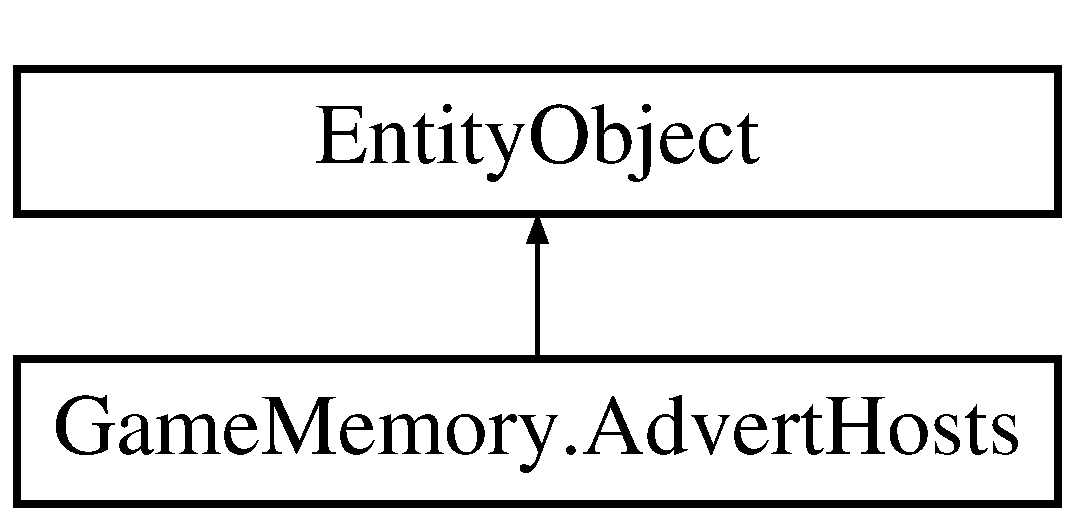
\includegraphics[height=2.000000cm]{class_game_memory_1_1_advert_hosts}
\end{center}
\end{figure}
\subsection*{Static Public Member Functions}
\begin{DoxyCompactItemize}
\item 
static \hyperlink{class_game_memory_1_1_advert_hosts}{Advert\-Hosts} \hyperlink{class_game_memory_1_1_advert_hosts_a9d7c2ea42590dcf01fb28977a6552417}{Create\-Advert\-Hosts} (global\-::\-System.\-Int32 advert\-Host\-Id, global\-::\-System.\-Int32 advert\-Host\-Category\-Id, global\-::\-System.\-Int32 location\-Id, global\-::\-System.\-Boolean \hyperlink{class_game_memory_1_1_advert_hosts_a8d5395f4cef95ff9558134b2c37feb6b}{is\-Up})
\begin{DoxyCompactList}\small\item\em Crear un nuevo objeto \hyperlink{class_game_memory_1_1_advert_hosts}{Advert\-Hosts}. \end{DoxyCompactList}\end{DoxyCompactItemize}
\subsection*{Properties}
\begin{DoxyCompactItemize}
\item 
global\-::\-System.\-Int32 \hyperlink{class_game_memory_1_1_advert_hosts_a050c3c580d2c90577cabff79c565fdbc}{Advert\-Host\-Id}\hspace{0.3cm}{\ttfamily  \mbox{[}get, set\mbox{]}}
\begin{DoxyCompactList}\small\item\em No hay documentación de metadatos disponible. \end{DoxyCompactList}\item 
global\-::\-System.\-String \hyperlink{class_game_memory_1_1_advert_hosts_a5738204678324f4adb8a9b54c1331a08}{Advert\-Host\-Name}\hspace{0.3cm}{\ttfamily  \mbox{[}get, set\mbox{]}}
\begin{DoxyCompactList}\small\item\em No hay documentación de metadatos disponible. \end{DoxyCompactList}\item 
global\-::\-System.\-Int32 \hyperlink{class_game_memory_1_1_advert_hosts_adb9878a533fd009839d66c95d514e075}{Advert\-Host\-Category\-Id}\hspace{0.3cm}{\ttfamily  \mbox{[}get, set\mbox{]}}
\begin{DoxyCompactList}\small\item\em No hay documentación de metadatos disponible. \end{DoxyCompactList}\item 
Nullable$<$ global\-::\-System.\-Date\-Time $>$ \hyperlink{class_game_memory_1_1_advert_hosts_a01dfdd5bd9e5b5970ae3e2768f33e6d6}{Start\-Time}\hspace{0.3cm}{\ttfamily  \mbox{[}get, set\mbox{]}}
\begin{DoxyCompactList}\small\item\em No hay documentación de metadatos disponible. \end{DoxyCompactList}\item 
Nullable$<$ global\-::\-System.\-Date\-Time $>$ \hyperlink{class_game_memory_1_1_advert_hosts_a565c137468bd134b1fa5c32a9f32f9c0}{End\-Time}\hspace{0.3cm}{\ttfamily  \mbox{[}get, set\mbox{]}}
\begin{DoxyCompactList}\small\item\em No hay documentación de metadatos disponible. \end{DoxyCompactList}\item 
Nullable$<$ global\-::\-System.\-Date\-Time $>$ \hyperlink{class_game_memory_1_1_advert_hosts_ae2a1fcae997b086b7029ae2739f69a8a}{Last\-Down\-Time}\hspace{0.3cm}{\ttfamily  \mbox{[}get, set\mbox{]}}
\begin{DoxyCompactList}\small\item\em No hay documentación de metadatos disponible. \end{DoxyCompactList}\item 
Nullable$<$ global\-::\-System.\-Date\-Time $>$ \hyperlink{class_game_memory_1_1_advert_hosts_ac9286ac99bf2f9237cdf0ade0823ad81}{Last\-Up\-Time}\hspace{0.3cm}{\ttfamily  \mbox{[}get, set\mbox{]}}
\begin{DoxyCompactList}\small\item\em No hay documentación de metadatos disponible. \end{DoxyCompactList}\item 
Nullable$<$ global\-::\-System.\-Date\-Time $>$ \hyperlink{class_game_memory_1_1_advert_hosts_a60aaa40a77a9d9a4df8f3e05df660496}{Up\-Time}\hspace{0.3cm}{\ttfamily  \mbox{[}get, set\mbox{]}}
\begin{DoxyCompactList}\small\item\em No hay documentación de metadatos disponible. \end{DoxyCompactList}\item 
global\-::\-System.\-Int32 \hyperlink{class_game_memory_1_1_advert_hosts_a001106f5700ae6ddd8db5d749eeceb52}{Location\-Id}\hspace{0.3cm}{\ttfamily  \mbox{[}get, set\mbox{]}}
\begin{DoxyCompactList}\small\item\em No hay documentación de metadatos disponible. \end{DoxyCompactList}\item 
global\-::\-System.\-String \hyperlink{class_game_memory_1_1_advert_hosts_ac6a05cfb2749577b3b7918777ef0f820}{Kinect\-I\-D}\hspace{0.3cm}{\ttfamily  \mbox{[}get, set\mbox{]}}
\begin{DoxyCompactList}\small\item\em No hay documentación de metadatos disponible. \end{DoxyCompactList}\item 
global\-::\-System.\-Boolean \hyperlink{class_game_memory_1_1_advert_hosts_a8d5395f4cef95ff9558134b2c37feb6b}{is\-Up}\hspace{0.3cm}{\ttfamily  \mbox{[}get, set\mbox{]}}
\begin{DoxyCompactList}\small\item\em No hay documentación de metadatos disponible. \end{DoxyCompactList}\item 
Nullable$<$ global\-::\-System.\-Int32 $>$ \hyperlink{class_game_memory_1_1_advert_hosts_afa83e1eed2d680e2b5025fc5a79562dc}{Campaign\-Location\-\_\-\-Campaign\-Location\-Id}\hspace{0.3cm}{\ttfamily  \mbox{[}get, set\mbox{]}}
\begin{DoxyCompactList}\small\item\em No hay documentación de metadatos disponible. \end{DoxyCompactList}\item 
Nullable$<$ global\-::\-System.\-Int32 $>$ \hyperlink{class_game_memory_1_1_advert_hosts_af853b0ead0e1a677765d61f294615155}{Advert\-Campaign\-\_\-\-Advert\-Campaign\-Id}\hspace{0.3cm}{\ttfamily  \mbox{[}get, set\mbox{]}}
\begin{DoxyCompactList}\small\item\em No hay documentación de metadatos disponible. \end{DoxyCompactList}\item 
\hyperlink{class_game_memory_1_1_advert_campaigns}{Advert\-Campaigns} \hyperlink{class_game_memory_1_1_advert_hosts_a156a61056fa542946f9e4f130cef3a0c}{Advert\-Campaigns}\hspace{0.3cm}{\ttfamily  \mbox{[}get, set\mbox{]}}
\begin{DoxyCompactList}\small\item\em No hay documentación de metadatos disponible. \end{DoxyCompactList}\item 
Entity\-Reference$<$ \hyperlink{class_game_memory_1_1_advert_campaigns}{Advert\-Campaigns} $>$ \hyperlink{class_game_memory_1_1_advert_hosts_ac1362cf9f56041ecda1da4beee7cd9b2}{Advert\-Campaigns\-Reference}\hspace{0.3cm}{\ttfamily  \mbox{[}get, set\mbox{]}}
\begin{DoxyCompactList}\small\item\em No hay documentación de metadatos disponible. \end{DoxyCompactList}\item 
\hyperlink{class_game_memory_1_1_advert_host_categories}{Advert\-Host\-Categories} \hyperlink{class_game_memory_1_1_advert_hosts_ac76d2a1c64a2108e2caeb0ba0ec783eb}{Advert\-Host\-Categories}\hspace{0.3cm}{\ttfamily  \mbox{[}get, set\mbox{]}}
\begin{DoxyCompactList}\small\item\em No hay documentación de metadatos disponible. \end{DoxyCompactList}\item 
Entity\-Reference\\*
$<$ \hyperlink{class_game_memory_1_1_advert_host_categories}{Advert\-Host\-Categories} $>$ \hyperlink{class_game_memory_1_1_advert_hosts_a90144e6cd1a7c13e64a210d9fb84bb30}{Advert\-Host\-Categories\-Reference}\hspace{0.3cm}{\ttfamily  \mbox{[}get, set\mbox{]}}
\begin{DoxyCompactList}\small\item\em No hay documentación de metadatos disponible. \end{DoxyCompactList}\item 
\hyperlink{class_game_memory_1_1_campaign_locations}{Campaign\-Locations} \hyperlink{class_game_memory_1_1_advert_hosts_ab5cafcddf70eae65c6848c168af5a4e5}{Campaign\-Locations}\hspace{0.3cm}{\ttfamily  \mbox{[}get, set\mbox{]}}
\begin{DoxyCompactList}\small\item\em No hay documentación de metadatos disponible. \end{DoxyCompactList}\item 
Entity\-Reference\\*
$<$ \hyperlink{class_game_memory_1_1_campaign_locations}{Campaign\-Locations} $>$ \hyperlink{class_game_memory_1_1_advert_hosts_adde1f5e205d40e2b0893edd68382747a}{Campaign\-Locations\-Reference}\hspace{0.3cm}{\ttfamily  \mbox{[}get, set\mbox{]}}
\begin{DoxyCompactList}\small\item\em No hay documentación de metadatos disponible. \end{DoxyCompactList}\item 
\hyperlink{class_game_memory_1_1_locations}{Locations} \hyperlink{class_game_memory_1_1_advert_hosts_aecffc47c6b7f5efa56310dda35ef0924}{Locations}\hspace{0.3cm}{\ttfamily  \mbox{[}get, set\mbox{]}}
\begin{DoxyCompactList}\small\item\em No hay documentación de metadatos disponible. \end{DoxyCompactList}\item 
Entity\-Reference$<$ \hyperlink{class_game_memory_1_1_locations}{Locations} $>$ \hyperlink{class_game_memory_1_1_advert_hosts_a718933a989867b5853054036455233f3}{Locations\-Reference}\hspace{0.3cm}{\ttfamily  \mbox{[}get, set\mbox{]}}
\begin{DoxyCompactList}\small\item\em No hay documentación de metadatos disponible. \end{DoxyCompactList}\item 
Entity\-Collection$<$ \hyperlink{class_game_memory_1_1_monitorings}{Monitorings} $>$ \hyperlink{class_game_memory_1_1_advert_hosts_a19750c448c029de2b56be189f62245bf}{Monitorings}\hspace{0.3cm}{\ttfamily  \mbox{[}get, set\mbox{]}}
\begin{DoxyCompactList}\small\item\em No hay documentación de metadatos disponible. \end{DoxyCompactList}\end{DoxyCompactItemize}


\subsection{Detailed Description}
No hay documentación de metadatos disponible. 



\subsection{Member Function Documentation}
\hypertarget{class_game_memory_1_1_advert_hosts_a9d7c2ea42590dcf01fb28977a6552417}{\index{Game\-Memory\-::\-Advert\-Hosts@{Game\-Memory\-::\-Advert\-Hosts}!Create\-Advert\-Hosts@{Create\-Advert\-Hosts}}
\index{Create\-Advert\-Hosts@{Create\-Advert\-Hosts}!GameMemory::AdvertHosts@{Game\-Memory\-::\-Advert\-Hosts}}
\subsubsection[{Create\-Advert\-Hosts}]{\setlength{\rightskip}{0pt plus 5cm}static {\bf Advert\-Hosts} Game\-Memory.\-Advert\-Hosts.\-Create\-Advert\-Hosts (
\begin{DoxyParamCaption}
\item[{global\-::\-System.\-Int32}]{advert\-Host\-Id, }
\item[{global\-::\-System.\-Int32}]{advert\-Host\-Category\-Id, }
\item[{global\-::\-System.\-Int32}]{location\-Id, }
\item[{global\-::\-System.\-Boolean}]{is\-Up}
\end{DoxyParamCaption}
)\hspace{0.3cm}{\ttfamily [static]}}}\label{class_game_memory_1_1_advert_hosts_a9d7c2ea42590dcf01fb28977a6552417}


Crear un nuevo objeto \hyperlink{class_game_memory_1_1_advert_hosts}{Advert\-Hosts}. 


\begin{DoxyParams}{Parameters}
{\em advert\-Host\-Id} & Valor inicial de la propiedad Advert\-Host\-Id.\\
\hline
{\em advert\-Host\-Category\-Id} & Valor inicial de la propiedad Advert\-Host\-Category\-Id.\\
\hline
{\em location\-Id} & Valor inicial de la propiedad Location\-Id.\\
\hline
{\em is\-Up} & Valor inicial de la propiedad is\-Up.\\
\hline
\end{DoxyParams}


\subsection{Property Documentation}
\hypertarget{class_game_memory_1_1_advert_hosts_af853b0ead0e1a677765d61f294615155}{\index{Game\-Memory\-::\-Advert\-Hosts@{Game\-Memory\-::\-Advert\-Hosts}!Advert\-Campaign\-\_\-\-Advert\-Campaign\-Id@{Advert\-Campaign\-\_\-\-Advert\-Campaign\-Id}}
\index{Advert\-Campaign\-\_\-\-Advert\-Campaign\-Id@{Advert\-Campaign\-\_\-\-Advert\-Campaign\-Id}!GameMemory::AdvertHosts@{Game\-Memory\-::\-Advert\-Hosts}}
\subsubsection[{Advert\-Campaign\-\_\-\-Advert\-Campaign\-Id}]{\setlength{\rightskip}{0pt plus 5cm}Nullable$<$global.\-System.\-Int32$>$ Game\-Memory.\-Advert\-Hosts.\-Advert\-Campaign\-\_\-\-Advert\-Campaign\-Id\hspace{0.3cm}{\ttfamily [get]}, {\ttfamily [set]}}}\label{class_game_memory_1_1_advert_hosts_af853b0ead0e1a677765d61f294615155}


No hay documentación de metadatos disponible. 

\hypertarget{class_game_memory_1_1_advert_hosts_a156a61056fa542946f9e4f130cef3a0c}{\index{Game\-Memory\-::\-Advert\-Hosts@{Game\-Memory\-::\-Advert\-Hosts}!Advert\-Campaigns@{Advert\-Campaigns}}
\index{Advert\-Campaigns@{Advert\-Campaigns}!GameMemory::AdvertHosts@{Game\-Memory\-::\-Advert\-Hosts}}
\subsubsection[{Advert\-Campaigns}]{\setlength{\rightskip}{0pt plus 5cm}{\bf Advert\-Campaigns} Game\-Memory.\-Advert\-Hosts.\-Advert\-Campaigns\hspace{0.3cm}{\ttfamily [get]}, {\ttfamily [set]}}}\label{class_game_memory_1_1_advert_hosts_a156a61056fa542946f9e4f130cef3a0c}


No hay documentación de metadatos disponible. 

\hypertarget{class_game_memory_1_1_advert_hosts_ac1362cf9f56041ecda1da4beee7cd9b2}{\index{Game\-Memory\-::\-Advert\-Hosts@{Game\-Memory\-::\-Advert\-Hosts}!Advert\-Campaigns\-Reference@{Advert\-Campaigns\-Reference}}
\index{Advert\-Campaigns\-Reference@{Advert\-Campaigns\-Reference}!GameMemory::AdvertHosts@{Game\-Memory\-::\-Advert\-Hosts}}
\subsubsection[{Advert\-Campaigns\-Reference}]{\setlength{\rightskip}{0pt plus 5cm}Entity\-Reference$<${\bf Advert\-Campaigns}$>$ Game\-Memory.\-Advert\-Hosts.\-Advert\-Campaigns\-Reference\hspace{0.3cm}{\ttfamily [get]}, {\ttfamily [set]}}}\label{class_game_memory_1_1_advert_hosts_ac1362cf9f56041ecda1da4beee7cd9b2}


No hay documentación de metadatos disponible. 

\hypertarget{class_game_memory_1_1_advert_hosts_ac76d2a1c64a2108e2caeb0ba0ec783eb}{\index{Game\-Memory\-::\-Advert\-Hosts@{Game\-Memory\-::\-Advert\-Hosts}!Advert\-Host\-Categories@{Advert\-Host\-Categories}}
\index{Advert\-Host\-Categories@{Advert\-Host\-Categories}!GameMemory::AdvertHosts@{Game\-Memory\-::\-Advert\-Hosts}}
\subsubsection[{Advert\-Host\-Categories}]{\setlength{\rightskip}{0pt plus 5cm}{\bf Advert\-Host\-Categories} Game\-Memory.\-Advert\-Hosts.\-Advert\-Host\-Categories\hspace{0.3cm}{\ttfamily [get]}, {\ttfamily [set]}}}\label{class_game_memory_1_1_advert_hosts_ac76d2a1c64a2108e2caeb0ba0ec783eb}


No hay documentación de metadatos disponible. 

\hypertarget{class_game_memory_1_1_advert_hosts_a90144e6cd1a7c13e64a210d9fb84bb30}{\index{Game\-Memory\-::\-Advert\-Hosts@{Game\-Memory\-::\-Advert\-Hosts}!Advert\-Host\-Categories\-Reference@{Advert\-Host\-Categories\-Reference}}
\index{Advert\-Host\-Categories\-Reference@{Advert\-Host\-Categories\-Reference}!GameMemory::AdvertHosts@{Game\-Memory\-::\-Advert\-Hosts}}
\subsubsection[{Advert\-Host\-Categories\-Reference}]{\setlength{\rightskip}{0pt plus 5cm}Entity\-Reference$<${\bf Advert\-Host\-Categories}$>$ Game\-Memory.\-Advert\-Hosts.\-Advert\-Host\-Categories\-Reference\hspace{0.3cm}{\ttfamily [get]}, {\ttfamily [set]}}}\label{class_game_memory_1_1_advert_hosts_a90144e6cd1a7c13e64a210d9fb84bb30}


No hay documentación de metadatos disponible. 

\hypertarget{class_game_memory_1_1_advert_hosts_adb9878a533fd009839d66c95d514e075}{\index{Game\-Memory\-::\-Advert\-Hosts@{Game\-Memory\-::\-Advert\-Hosts}!Advert\-Host\-Category\-Id@{Advert\-Host\-Category\-Id}}
\index{Advert\-Host\-Category\-Id@{Advert\-Host\-Category\-Id}!GameMemory::AdvertHosts@{Game\-Memory\-::\-Advert\-Hosts}}
\subsubsection[{Advert\-Host\-Category\-Id}]{\setlength{\rightskip}{0pt plus 5cm}global.\-System.\-Int32 Game\-Memory.\-Advert\-Hosts.\-Advert\-Host\-Category\-Id\hspace{0.3cm}{\ttfamily [get]}, {\ttfamily [set]}}}\label{class_game_memory_1_1_advert_hosts_adb9878a533fd009839d66c95d514e075}


No hay documentación de metadatos disponible. 

\hypertarget{class_game_memory_1_1_advert_hosts_a050c3c580d2c90577cabff79c565fdbc}{\index{Game\-Memory\-::\-Advert\-Hosts@{Game\-Memory\-::\-Advert\-Hosts}!Advert\-Host\-Id@{Advert\-Host\-Id}}
\index{Advert\-Host\-Id@{Advert\-Host\-Id}!GameMemory::AdvertHosts@{Game\-Memory\-::\-Advert\-Hosts}}
\subsubsection[{Advert\-Host\-Id}]{\setlength{\rightskip}{0pt plus 5cm}global.\-System.\-Int32 Game\-Memory.\-Advert\-Hosts.\-Advert\-Host\-Id\hspace{0.3cm}{\ttfamily [get]}, {\ttfamily [set]}}}\label{class_game_memory_1_1_advert_hosts_a050c3c580d2c90577cabff79c565fdbc}


No hay documentación de metadatos disponible. 

\hypertarget{class_game_memory_1_1_advert_hosts_a5738204678324f4adb8a9b54c1331a08}{\index{Game\-Memory\-::\-Advert\-Hosts@{Game\-Memory\-::\-Advert\-Hosts}!Advert\-Host\-Name@{Advert\-Host\-Name}}
\index{Advert\-Host\-Name@{Advert\-Host\-Name}!GameMemory::AdvertHosts@{Game\-Memory\-::\-Advert\-Hosts}}
\subsubsection[{Advert\-Host\-Name}]{\setlength{\rightskip}{0pt plus 5cm}global.\-System.\-String Game\-Memory.\-Advert\-Hosts.\-Advert\-Host\-Name\hspace{0.3cm}{\ttfamily [get]}, {\ttfamily [set]}}}\label{class_game_memory_1_1_advert_hosts_a5738204678324f4adb8a9b54c1331a08}


No hay documentación de metadatos disponible. 

\hypertarget{class_game_memory_1_1_advert_hosts_afa83e1eed2d680e2b5025fc5a79562dc}{\index{Game\-Memory\-::\-Advert\-Hosts@{Game\-Memory\-::\-Advert\-Hosts}!Campaign\-Location\-\_\-\-Campaign\-Location\-Id@{Campaign\-Location\-\_\-\-Campaign\-Location\-Id}}
\index{Campaign\-Location\-\_\-\-Campaign\-Location\-Id@{Campaign\-Location\-\_\-\-Campaign\-Location\-Id}!GameMemory::AdvertHosts@{Game\-Memory\-::\-Advert\-Hosts}}
\subsubsection[{Campaign\-Location\-\_\-\-Campaign\-Location\-Id}]{\setlength{\rightskip}{0pt plus 5cm}Nullable$<$global.\-System.\-Int32$>$ Game\-Memory.\-Advert\-Hosts.\-Campaign\-Location\-\_\-\-Campaign\-Location\-Id\hspace{0.3cm}{\ttfamily [get]}, {\ttfamily [set]}}}\label{class_game_memory_1_1_advert_hosts_afa83e1eed2d680e2b5025fc5a79562dc}


No hay documentación de metadatos disponible. 

\hypertarget{class_game_memory_1_1_advert_hosts_ab5cafcddf70eae65c6848c168af5a4e5}{\index{Game\-Memory\-::\-Advert\-Hosts@{Game\-Memory\-::\-Advert\-Hosts}!Campaign\-Locations@{Campaign\-Locations}}
\index{Campaign\-Locations@{Campaign\-Locations}!GameMemory::AdvertHosts@{Game\-Memory\-::\-Advert\-Hosts}}
\subsubsection[{Campaign\-Locations}]{\setlength{\rightskip}{0pt plus 5cm}{\bf Campaign\-Locations} Game\-Memory.\-Advert\-Hosts.\-Campaign\-Locations\hspace{0.3cm}{\ttfamily [get]}, {\ttfamily [set]}}}\label{class_game_memory_1_1_advert_hosts_ab5cafcddf70eae65c6848c168af5a4e5}


No hay documentación de metadatos disponible. 

\hypertarget{class_game_memory_1_1_advert_hosts_adde1f5e205d40e2b0893edd68382747a}{\index{Game\-Memory\-::\-Advert\-Hosts@{Game\-Memory\-::\-Advert\-Hosts}!Campaign\-Locations\-Reference@{Campaign\-Locations\-Reference}}
\index{Campaign\-Locations\-Reference@{Campaign\-Locations\-Reference}!GameMemory::AdvertHosts@{Game\-Memory\-::\-Advert\-Hosts}}
\subsubsection[{Campaign\-Locations\-Reference}]{\setlength{\rightskip}{0pt plus 5cm}Entity\-Reference$<${\bf Campaign\-Locations}$>$ Game\-Memory.\-Advert\-Hosts.\-Campaign\-Locations\-Reference\hspace{0.3cm}{\ttfamily [get]}, {\ttfamily [set]}}}\label{class_game_memory_1_1_advert_hosts_adde1f5e205d40e2b0893edd68382747a}


No hay documentación de metadatos disponible. 

\hypertarget{class_game_memory_1_1_advert_hosts_a565c137468bd134b1fa5c32a9f32f9c0}{\index{Game\-Memory\-::\-Advert\-Hosts@{Game\-Memory\-::\-Advert\-Hosts}!End\-Time@{End\-Time}}
\index{End\-Time@{End\-Time}!GameMemory::AdvertHosts@{Game\-Memory\-::\-Advert\-Hosts}}
\subsubsection[{End\-Time}]{\setlength{\rightskip}{0pt plus 5cm}Nullable$<$global.\-System.\-Date\-Time$>$ Game\-Memory.\-Advert\-Hosts.\-End\-Time\hspace{0.3cm}{\ttfamily [get]}, {\ttfamily [set]}}}\label{class_game_memory_1_1_advert_hosts_a565c137468bd134b1fa5c32a9f32f9c0}


No hay documentación de metadatos disponible. 

\hypertarget{class_game_memory_1_1_advert_hosts_a8d5395f4cef95ff9558134b2c37feb6b}{\index{Game\-Memory\-::\-Advert\-Hosts@{Game\-Memory\-::\-Advert\-Hosts}!is\-Up@{is\-Up}}
\index{is\-Up@{is\-Up}!GameMemory::AdvertHosts@{Game\-Memory\-::\-Advert\-Hosts}}
\subsubsection[{is\-Up}]{\setlength{\rightskip}{0pt plus 5cm}global.\-System.\-Boolean Game\-Memory.\-Advert\-Hosts.\-is\-Up\hspace{0.3cm}{\ttfamily [get]}, {\ttfamily [set]}}}\label{class_game_memory_1_1_advert_hosts_a8d5395f4cef95ff9558134b2c37feb6b}


No hay documentación de metadatos disponible. 

\hypertarget{class_game_memory_1_1_advert_hosts_ac6a05cfb2749577b3b7918777ef0f820}{\index{Game\-Memory\-::\-Advert\-Hosts@{Game\-Memory\-::\-Advert\-Hosts}!Kinect\-I\-D@{Kinect\-I\-D}}
\index{Kinect\-I\-D@{Kinect\-I\-D}!GameMemory::AdvertHosts@{Game\-Memory\-::\-Advert\-Hosts}}
\subsubsection[{Kinect\-I\-D}]{\setlength{\rightskip}{0pt plus 5cm}global.\-System.\-String Game\-Memory.\-Advert\-Hosts.\-Kinect\-I\-D\hspace{0.3cm}{\ttfamily [get]}, {\ttfamily [set]}}}\label{class_game_memory_1_1_advert_hosts_ac6a05cfb2749577b3b7918777ef0f820}


No hay documentación de metadatos disponible. 

\hypertarget{class_game_memory_1_1_advert_hosts_ae2a1fcae997b086b7029ae2739f69a8a}{\index{Game\-Memory\-::\-Advert\-Hosts@{Game\-Memory\-::\-Advert\-Hosts}!Last\-Down\-Time@{Last\-Down\-Time}}
\index{Last\-Down\-Time@{Last\-Down\-Time}!GameMemory::AdvertHosts@{Game\-Memory\-::\-Advert\-Hosts}}
\subsubsection[{Last\-Down\-Time}]{\setlength{\rightskip}{0pt plus 5cm}Nullable$<$global.\-System.\-Date\-Time$>$ Game\-Memory.\-Advert\-Hosts.\-Last\-Down\-Time\hspace{0.3cm}{\ttfamily [get]}, {\ttfamily [set]}}}\label{class_game_memory_1_1_advert_hosts_ae2a1fcae997b086b7029ae2739f69a8a}


No hay documentación de metadatos disponible. 

\hypertarget{class_game_memory_1_1_advert_hosts_ac9286ac99bf2f9237cdf0ade0823ad81}{\index{Game\-Memory\-::\-Advert\-Hosts@{Game\-Memory\-::\-Advert\-Hosts}!Last\-Up\-Time@{Last\-Up\-Time}}
\index{Last\-Up\-Time@{Last\-Up\-Time}!GameMemory::AdvertHosts@{Game\-Memory\-::\-Advert\-Hosts}}
\subsubsection[{Last\-Up\-Time}]{\setlength{\rightskip}{0pt plus 5cm}Nullable$<$global.\-System.\-Date\-Time$>$ Game\-Memory.\-Advert\-Hosts.\-Last\-Up\-Time\hspace{0.3cm}{\ttfamily [get]}, {\ttfamily [set]}}}\label{class_game_memory_1_1_advert_hosts_ac9286ac99bf2f9237cdf0ade0823ad81}


No hay documentación de metadatos disponible. 

\hypertarget{class_game_memory_1_1_advert_hosts_a001106f5700ae6ddd8db5d749eeceb52}{\index{Game\-Memory\-::\-Advert\-Hosts@{Game\-Memory\-::\-Advert\-Hosts}!Location\-Id@{Location\-Id}}
\index{Location\-Id@{Location\-Id}!GameMemory::AdvertHosts@{Game\-Memory\-::\-Advert\-Hosts}}
\subsubsection[{Location\-Id}]{\setlength{\rightskip}{0pt plus 5cm}global.\-System.\-Int32 Game\-Memory.\-Advert\-Hosts.\-Location\-Id\hspace{0.3cm}{\ttfamily [get]}, {\ttfamily [set]}}}\label{class_game_memory_1_1_advert_hosts_a001106f5700ae6ddd8db5d749eeceb52}


No hay documentación de metadatos disponible. 

\hypertarget{class_game_memory_1_1_advert_hosts_aecffc47c6b7f5efa56310dda35ef0924}{\index{Game\-Memory\-::\-Advert\-Hosts@{Game\-Memory\-::\-Advert\-Hosts}!Locations@{Locations}}
\index{Locations@{Locations}!GameMemory::AdvertHosts@{Game\-Memory\-::\-Advert\-Hosts}}
\subsubsection[{Locations}]{\setlength{\rightskip}{0pt plus 5cm}{\bf Locations} Game\-Memory.\-Advert\-Hosts.\-Locations\hspace{0.3cm}{\ttfamily [get]}, {\ttfamily [set]}}}\label{class_game_memory_1_1_advert_hosts_aecffc47c6b7f5efa56310dda35ef0924}


No hay documentación de metadatos disponible. 

\hypertarget{class_game_memory_1_1_advert_hosts_a718933a989867b5853054036455233f3}{\index{Game\-Memory\-::\-Advert\-Hosts@{Game\-Memory\-::\-Advert\-Hosts}!Locations\-Reference@{Locations\-Reference}}
\index{Locations\-Reference@{Locations\-Reference}!GameMemory::AdvertHosts@{Game\-Memory\-::\-Advert\-Hosts}}
\subsubsection[{Locations\-Reference}]{\setlength{\rightskip}{0pt plus 5cm}Entity\-Reference$<${\bf Locations}$>$ Game\-Memory.\-Advert\-Hosts.\-Locations\-Reference\hspace{0.3cm}{\ttfamily [get]}, {\ttfamily [set]}}}\label{class_game_memory_1_1_advert_hosts_a718933a989867b5853054036455233f3}


No hay documentación de metadatos disponible. 

\hypertarget{class_game_memory_1_1_advert_hosts_a19750c448c029de2b56be189f62245bf}{\index{Game\-Memory\-::\-Advert\-Hosts@{Game\-Memory\-::\-Advert\-Hosts}!Monitorings@{Monitorings}}
\index{Monitorings@{Monitorings}!GameMemory::AdvertHosts@{Game\-Memory\-::\-Advert\-Hosts}}
\subsubsection[{Monitorings}]{\setlength{\rightskip}{0pt plus 5cm}Entity\-Collection$<${\bf Monitorings}$>$ Game\-Memory.\-Advert\-Hosts.\-Monitorings\hspace{0.3cm}{\ttfamily [get]}, {\ttfamily [set]}}}\label{class_game_memory_1_1_advert_hosts_a19750c448c029de2b56be189f62245bf}


No hay documentación de metadatos disponible. 

\hypertarget{class_game_memory_1_1_advert_hosts_a01dfdd5bd9e5b5970ae3e2768f33e6d6}{\index{Game\-Memory\-::\-Advert\-Hosts@{Game\-Memory\-::\-Advert\-Hosts}!Start\-Time@{Start\-Time}}
\index{Start\-Time@{Start\-Time}!GameMemory::AdvertHosts@{Game\-Memory\-::\-Advert\-Hosts}}
\subsubsection[{Start\-Time}]{\setlength{\rightskip}{0pt plus 5cm}Nullable$<$global.\-System.\-Date\-Time$>$ Game\-Memory.\-Advert\-Hosts.\-Start\-Time\hspace{0.3cm}{\ttfamily [get]}, {\ttfamily [set]}}}\label{class_game_memory_1_1_advert_hosts_a01dfdd5bd9e5b5970ae3e2768f33e6d6}


No hay documentación de metadatos disponible. 

\hypertarget{class_game_memory_1_1_advert_hosts_a60aaa40a77a9d9a4df8f3e05df660496}{\index{Game\-Memory\-::\-Advert\-Hosts@{Game\-Memory\-::\-Advert\-Hosts}!Up\-Time@{Up\-Time}}
\index{Up\-Time@{Up\-Time}!GameMemory::AdvertHosts@{Game\-Memory\-::\-Advert\-Hosts}}
\subsubsection[{Up\-Time}]{\setlength{\rightskip}{0pt plus 5cm}Nullable$<$global.\-System.\-Date\-Time$>$ Game\-Memory.\-Advert\-Hosts.\-Up\-Time\hspace{0.3cm}{\ttfamily [get]}, {\ttfamily [set]}}}\label{class_game_memory_1_1_advert_hosts_a60aaa40a77a9d9a4df8f3e05df660496}


No hay documentación de metadatos disponible. 



The documentation for this class was generated from the following file\-:\begin{DoxyCompactItemize}
\item 
D\-:/tesis\-Assembla/branches/\-Branch\-\_\-\-Tesis\-\_\-\-Sprint01/\-Dev/\-Interaction Module/\-Game\-Memory/\-Game\-Memory/O\-M\-K\-T.\-Designer.\-cs\end{DoxyCompactItemize}

\hypertarget{class_game_memory_1_1_adverts}{\section{Game\-Memory.\-Adverts Class Reference}
\label{class_game_memory_1_1_adverts}\index{Game\-Memory.\-Adverts@{Game\-Memory.\-Adverts}}
}


No hay documentación de metadatos disponible.  


Inheritance diagram for Game\-Memory.\-Adverts\-:\begin{figure}[H]
\begin{center}
\leavevmode
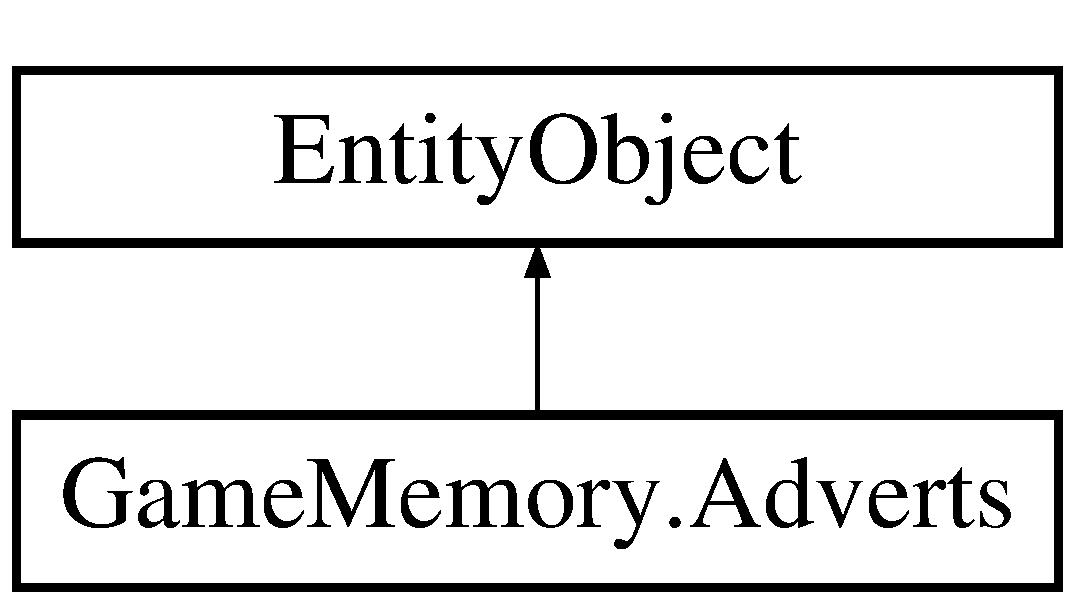
\includegraphics[height=2.000000cm]{class_game_memory_1_1_adverts}
\end{center}
\end{figure}
\subsection*{Static Public Member Functions}
\begin{DoxyCompactItemize}
\item 
static \hyperlink{class_game_memory_1_1_adverts}{Adverts} \hyperlink{class_game_memory_1_1_adverts_a7a0587b12eea6e049be8282653ad83a6}{Create\-Adverts} (global\-::\-System.\-Int32 advert\-Id, global\-::\-System.\-Int32 advert\-Type\-Id, global\-::\-System.\-Int32 advert\-State\-Id, global\-::\-System.\-String discriminator)
\begin{DoxyCompactList}\small\item\em Crear un nuevo objeto \hyperlink{class_game_memory_1_1_adverts}{Adverts}. \end{DoxyCompactList}\end{DoxyCompactItemize}
\subsection*{Properties}
\begin{DoxyCompactItemize}
\item 
global\-::\-System.\-Int32 \hyperlink{class_game_memory_1_1_adverts_ae0e7ff2ba8cd7a48717cd4b26a7927f1}{Advert\-Id}\hspace{0.3cm}{\ttfamily  \mbox{[}get, set\mbox{]}}
\begin{DoxyCompactList}\small\item\em No hay documentación de metadatos disponible. \end{DoxyCompactList}\item 
global\-::\-System.\-String \hyperlink{class_game_memory_1_1_adverts_a71dad8d0f7b7aa11e38a2f85a15615f3}{Name}\hspace{0.3cm}{\ttfamily  \mbox{[}get, set\mbox{]}}
\begin{DoxyCompactList}\small\item\em No hay documentación de metadatos disponible. \end{DoxyCompactList}\item 
global\-::\-System.\-Int32 \hyperlink{class_game_memory_1_1_adverts_a8c76ff553e2ab7355a2a470325146cff}{Advert\-Type\-Id}\hspace{0.3cm}{\ttfamily  \mbox{[}get, set\mbox{]}}
\begin{DoxyCompactList}\small\item\em No hay documentación de metadatos disponible. \end{DoxyCompactList}\item 
Nullable$<$ global\-::\-System.\-Date\-Time $>$ \hyperlink{class_game_memory_1_1_adverts_a25bc849ff293d51367af7f4a00da7c63}{Last\-Update}\hspace{0.3cm}{\ttfamily  \mbox{[}get, set\mbox{]}}
\begin{DoxyCompactList}\small\item\em No hay documentación de metadatos disponible. \end{DoxyCompactList}\item 
Nullable$<$ global\-::\-System.\-Date\-Time $>$ \hyperlink{class_game_memory_1_1_adverts_a21ad5dcffdf8c9b233901c6b55197e48}{End\-Datetime}\hspace{0.3cm}{\ttfamily  \mbox{[}get, set\mbox{]}}
\begin{DoxyCompactList}\small\item\em No hay documentación de metadatos disponible. \end{DoxyCompactList}\item 
Nullable$<$ global\-::\-System.\-Date\-Time $>$ \hyperlink{class_game_memory_1_1_adverts_a6f50aaad65f26ececf1f0e9d69dc006a}{Start\-Datetime}\hspace{0.3cm}{\ttfamily  \mbox{[}get, set\mbox{]}}
\begin{DoxyCompactList}\small\item\em No hay documentación de metadatos disponible. \end{DoxyCompactList}\item 
Nullable$<$ global\-::\-System.\-Date\-Time $>$ \hyperlink{class_game_memory_1_1_adverts_a52b3de606dfe54c1fe35ea83a53d42e6}{Created\-Date}\hspace{0.3cm}{\ttfamily  \mbox{[}get, set\mbox{]}}
\begin{DoxyCompactList}\small\item\em No hay documentación de metadatos disponible. \end{DoxyCompactList}\item 
global\-::\-System.\-Int32 \hyperlink{class_game_memory_1_1_adverts_a76a43f9edd08d0588a03cb95d6be0bcf}{Advert\-State\-Id}\hspace{0.3cm}{\ttfamily  \mbox{[}get, set\mbox{]}}
\begin{DoxyCompactList}\small\item\em No hay documentación de metadatos disponible. \end{DoxyCompactList}\item 
Nullable$<$ global\-::\-System.\-Int32 $>$ \hyperlink{class_game_memory_1_1_adverts_af3a5c0ddac27db7dd0bbf88ac1b250df}{Oportunities}\hspace{0.3cm}{\ttfamily  \mbox{[}get, set\mbox{]}}
\begin{DoxyCompactList}\small\item\em No hay documentación de metadatos disponible. \end{DoxyCompactList}\item 
Nullable$<$ global\-::\-System.\-Int32 $>$ \hyperlink{class_game_memory_1_1_adverts_a28c7f653f4c8f1d88ab3520408486ea3}{Sort\-Type\-Id}\hspace{0.3cm}{\ttfamily  \mbox{[}get, set\mbox{]}}
\begin{DoxyCompactList}\small\item\em No hay documentación de metadatos disponible. \end{DoxyCompactList}\item 
Nullable$<$ global\-::\-System.\-Boolean $>$ \hyperlink{class_game_memory_1_1_adverts_aef114b2666c933d5bba90f6a5def6e29}{Is\-Over}\hspace{0.3cm}{\ttfamily  \mbox{[}get, set\mbox{]}}
\begin{DoxyCompactList}\small\item\em No hay documentación de metadatos disponible. \end{DoxyCompactList}\item 
global\-::\-System.\-String \hyperlink{class_game_memory_1_1_adverts_a14b533de1869e89623ca3e4e6e9f7009}{Q\-R\-Code}\hspace{0.3cm}{\ttfamily  \mbox{[}get, set\mbox{]}}
\begin{DoxyCompactList}\small\item\em No hay documentación de metadatos disponible. \end{DoxyCompactList}\item 
global\-::\-System.\-String \hyperlink{class_game_memory_1_1_adverts_ad72413d0b9d943aadea17ebcb8b522ff}{Discriminator}\hspace{0.3cm}{\ttfamily  \mbox{[}get, set\mbox{]}}
\begin{DoxyCompactList}\small\item\em No hay documentación de metadatos disponible. \end{DoxyCompactList}\item 
Entity\-Collection\\*
$<$ \hyperlink{class_game_memory_1_1_advert_campaign_detail_interactions}{Advert\-Campaign\-Detail\-Interactions} $>$ \hyperlink{class_game_memory_1_1_adverts_a98057d3b841f0aa787406ff1f7111ce1}{Advert\-Campaign\-Detail\-Interactions}\hspace{0.3cm}{\ttfamily  \mbox{[}get, set\mbox{]}}
\begin{DoxyCompactList}\small\item\em No hay documentación de metadatos disponible. \end{DoxyCompactList}\item 
Entity\-Collection\\*
$<$ \hyperlink{class_game_memory_1_1_advert_campaign_details}{Advert\-Campaign\-Details} $>$ \hyperlink{class_game_memory_1_1_adverts_ada4c6a59fe3cddfeb554d415f894d742}{Advert\-Campaign\-Details}\hspace{0.3cm}{\ttfamily  \mbox{[}get, set\mbox{]}}
\begin{DoxyCompactList}\small\item\em No hay documentación de metadatos disponible. \end{DoxyCompactList}\item 
\hyperlink{class_game_memory_1_1_advert_states}{Advert\-States} \hyperlink{class_game_memory_1_1_adverts_ac01d784c797e36812eb383f4920bb276}{Advert\-States}\hspace{0.3cm}{\ttfamily  \mbox{[}get, set\mbox{]}}
\begin{DoxyCompactList}\small\item\em No hay documentación de metadatos disponible. \end{DoxyCompactList}\item 
Entity\-Reference$<$ \hyperlink{class_game_memory_1_1_advert_states}{Advert\-States} $>$ \hyperlink{class_game_memory_1_1_adverts_a5238fd71f38608ac56eb5eac5e0fe270}{Advert\-States\-Reference}\hspace{0.3cm}{\ttfamily  \mbox{[}get, set\mbox{]}}
\begin{DoxyCompactList}\small\item\em No hay documentación de metadatos disponible. \end{DoxyCompactList}\item 
\hyperlink{class_game_memory_1_1_advert_types}{Advert\-Types} \hyperlink{class_game_memory_1_1_adverts_a430fdeb87c0491d6a0c52aa2ce601673}{Advert\-Types}\hspace{0.3cm}{\ttfamily  \mbox{[}get, set\mbox{]}}
\begin{DoxyCompactList}\small\item\em No hay documentación de metadatos disponible. \end{DoxyCompactList}\item 
Entity\-Reference$<$ \hyperlink{class_game_memory_1_1_advert_types}{Advert\-Types} $>$ \hyperlink{class_game_memory_1_1_adverts_a12c5b442cf5e4ba2e320e1019aaaa5d5}{Advert\-Types\-Reference}\hspace{0.3cm}{\ttfamily  \mbox{[}get, set\mbox{]}}
\begin{DoxyCompactList}\small\item\em No hay documentación de metadatos disponible. \end{DoxyCompactList}\item 
\hyperlink{class_game_memory_1_1_sort_types}{Sort\-Types} \hyperlink{class_game_memory_1_1_adverts_a1466cfee905d0224c01bf20ef517ecfb}{Sort\-Types}\hspace{0.3cm}{\ttfamily  \mbox{[}get, set\mbox{]}}
\begin{DoxyCompactList}\small\item\em No hay documentación de metadatos disponible. \end{DoxyCompactList}\item 
Entity\-Reference$<$ \hyperlink{class_game_memory_1_1_sort_types}{Sort\-Types} $>$ \hyperlink{class_game_memory_1_1_adverts_a0e104d4a5eb16d3fe324396a2982eff3}{Sort\-Types\-Reference}\hspace{0.3cm}{\ttfamily  \mbox{[}get, set\mbox{]}}
\begin{DoxyCompactList}\small\item\em No hay documentación de metadatos disponible. \end{DoxyCompactList}\item 
Entity\-Collection$<$ \hyperlink{class_game_memory_1_1_catalog_details}{Catalog\-Details} $>$ \hyperlink{class_game_memory_1_1_adverts_a40a5ee6d3ab8ddb1d41ea4f5808dab5c}{Catalog\-Details}\hspace{0.3cm}{\ttfamily  \mbox{[}get, set\mbox{]}}
\begin{DoxyCompactList}\small\item\em No hay documentación de metadatos disponible. \end{DoxyCompactList}\item 
Entity\-Collection$<$ \hyperlink{class_game_memory_1_1_game_details}{Game\-Details} $>$ \hyperlink{class_game_memory_1_1_adverts_a5d5125df7fe34a0738042333e9ec5dc6}{Game\-Details}\hspace{0.3cm}{\ttfamily  \mbox{[}get, set\mbox{]}}
\begin{DoxyCompactList}\small\item\em No hay documentación de metadatos disponible. \end{DoxyCompactList}\end{DoxyCompactItemize}


\subsection{Detailed Description}
No hay documentación de metadatos disponible. 



\subsection{Member Function Documentation}
\hypertarget{class_game_memory_1_1_adverts_a7a0587b12eea6e049be8282653ad83a6}{\index{Game\-Memory\-::\-Adverts@{Game\-Memory\-::\-Adverts}!Create\-Adverts@{Create\-Adverts}}
\index{Create\-Adverts@{Create\-Adverts}!GameMemory::Adverts@{Game\-Memory\-::\-Adverts}}
\subsubsection[{Create\-Adverts}]{\setlength{\rightskip}{0pt plus 5cm}static {\bf Adverts} Game\-Memory.\-Adverts.\-Create\-Adverts (
\begin{DoxyParamCaption}
\item[{global\-::\-System.\-Int32}]{advert\-Id, }
\item[{global\-::\-System.\-Int32}]{advert\-Type\-Id, }
\item[{global\-::\-System.\-Int32}]{advert\-State\-Id, }
\item[{global\-::\-System.\-String}]{discriminator}
\end{DoxyParamCaption}
)\hspace{0.3cm}{\ttfamily [static]}}}\label{class_game_memory_1_1_adverts_a7a0587b12eea6e049be8282653ad83a6}


Crear un nuevo objeto \hyperlink{class_game_memory_1_1_adverts}{Adverts}. 


\begin{DoxyParams}{Parameters}
{\em advert\-Id} & Valor inicial de la propiedad Advert\-Id.\\
\hline
{\em advert\-Type\-Id} & Valor inicial de la propiedad Advert\-Type\-Id.\\
\hline
{\em advert\-State\-Id} & Valor inicial de la propiedad Advert\-State\-Id.\\
\hline
{\em discriminator} & Valor inicial de la propiedad Discriminator.\\
\hline
\end{DoxyParams}


\subsection{Property Documentation}
\hypertarget{class_game_memory_1_1_adverts_a98057d3b841f0aa787406ff1f7111ce1}{\index{Game\-Memory\-::\-Adverts@{Game\-Memory\-::\-Adverts}!Advert\-Campaign\-Detail\-Interactions@{Advert\-Campaign\-Detail\-Interactions}}
\index{Advert\-Campaign\-Detail\-Interactions@{Advert\-Campaign\-Detail\-Interactions}!GameMemory::Adverts@{Game\-Memory\-::\-Adverts}}
\subsubsection[{Advert\-Campaign\-Detail\-Interactions}]{\setlength{\rightskip}{0pt plus 5cm}Entity\-Collection$<${\bf Advert\-Campaign\-Detail\-Interactions}$>$ Game\-Memory.\-Adverts.\-Advert\-Campaign\-Detail\-Interactions\hspace{0.3cm}{\ttfamily [get]}, {\ttfamily [set]}}}\label{class_game_memory_1_1_adverts_a98057d3b841f0aa787406ff1f7111ce1}


No hay documentación de metadatos disponible. 

\hypertarget{class_game_memory_1_1_adverts_ada4c6a59fe3cddfeb554d415f894d742}{\index{Game\-Memory\-::\-Adverts@{Game\-Memory\-::\-Adverts}!Advert\-Campaign\-Details@{Advert\-Campaign\-Details}}
\index{Advert\-Campaign\-Details@{Advert\-Campaign\-Details}!GameMemory::Adverts@{Game\-Memory\-::\-Adverts}}
\subsubsection[{Advert\-Campaign\-Details}]{\setlength{\rightskip}{0pt plus 5cm}Entity\-Collection$<${\bf Advert\-Campaign\-Details}$>$ Game\-Memory.\-Adverts.\-Advert\-Campaign\-Details\hspace{0.3cm}{\ttfamily [get]}, {\ttfamily [set]}}}\label{class_game_memory_1_1_adverts_ada4c6a59fe3cddfeb554d415f894d742}


No hay documentación de metadatos disponible. 

\hypertarget{class_game_memory_1_1_adverts_ae0e7ff2ba8cd7a48717cd4b26a7927f1}{\index{Game\-Memory\-::\-Adverts@{Game\-Memory\-::\-Adverts}!Advert\-Id@{Advert\-Id}}
\index{Advert\-Id@{Advert\-Id}!GameMemory::Adverts@{Game\-Memory\-::\-Adverts}}
\subsubsection[{Advert\-Id}]{\setlength{\rightskip}{0pt plus 5cm}global.\-System.\-Int32 Game\-Memory.\-Adverts.\-Advert\-Id\hspace{0.3cm}{\ttfamily [get]}, {\ttfamily [set]}}}\label{class_game_memory_1_1_adverts_ae0e7ff2ba8cd7a48717cd4b26a7927f1}


No hay documentación de metadatos disponible. 

\hypertarget{class_game_memory_1_1_adverts_a76a43f9edd08d0588a03cb95d6be0bcf}{\index{Game\-Memory\-::\-Adverts@{Game\-Memory\-::\-Adverts}!Advert\-State\-Id@{Advert\-State\-Id}}
\index{Advert\-State\-Id@{Advert\-State\-Id}!GameMemory::Adverts@{Game\-Memory\-::\-Adverts}}
\subsubsection[{Advert\-State\-Id}]{\setlength{\rightskip}{0pt plus 5cm}global.\-System.\-Int32 Game\-Memory.\-Adverts.\-Advert\-State\-Id\hspace{0.3cm}{\ttfamily [get]}, {\ttfamily [set]}}}\label{class_game_memory_1_1_adverts_a76a43f9edd08d0588a03cb95d6be0bcf}


No hay documentación de metadatos disponible. 

\hypertarget{class_game_memory_1_1_adverts_ac01d784c797e36812eb383f4920bb276}{\index{Game\-Memory\-::\-Adverts@{Game\-Memory\-::\-Adverts}!Advert\-States@{Advert\-States}}
\index{Advert\-States@{Advert\-States}!GameMemory::Adverts@{Game\-Memory\-::\-Adverts}}
\subsubsection[{Advert\-States}]{\setlength{\rightskip}{0pt plus 5cm}{\bf Advert\-States} Game\-Memory.\-Adverts.\-Advert\-States\hspace{0.3cm}{\ttfamily [get]}, {\ttfamily [set]}}}\label{class_game_memory_1_1_adverts_ac01d784c797e36812eb383f4920bb276}


No hay documentación de metadatos disponible. 

\hypertarget{class_game_memory_1_1_adverts_a5238fd71f38608ac56eb5eac5e0fe270}{\index{Game\-Memory\-::\-Adverts@{Game\-Memory\-::\-Adverts}!Advert\-States\-Reference@{Advert\-States\-Reference}}
\index{Advert\-States\-Reference@{Advert\-States\-Reference}!GameMemory::Adverts@{Game\-Memory\-::\-Adverts}}
\subsubsection[{Advert\-States\-Reference}]{\setlength{\rightskip}{0pt plus 5cm}Entity\-Reference$<${\bf Advert\-States}$>$ Game\-Memory.\-Adverts.\-Advert\-States\-Reference\hspace{0.3cm}{\ttfamily [get]}, {\ttfamily [set]}}}\label{class_game_memory_1_1_adverts_a5238fd71f38608ac56eb5eac5e0fe270}


No hay documentación de metadatos disponible. 

\hypertarget{class_game_memory_1_1_adverts_a8c76ff553e2ab7355a2a470325146cff}{\index{Game\-Memory\-::\-Adverts@{Game\-Memory\-::\-Adverts}!Advert\-Type\-Id@{Advert\-Type\-Id}}
\index{Advert\-Type\-Id@{Advert\-Type\-Id}!GameMemory::Adverts@{Game\-Memory\-::\-Adverts}}
\subsubsection[{Advert\-Type\-Id}]{\setlength{\rightskip}{0pt plus 5cm}global.\-System.\-Int32 Game\-Memory.\-Adverts.\-Advert\-Type\-Id\hspace{0.3cm}{\ttfamily [get]}, {\ttfamily [set]}}}\label{class_game_memory_1_1_adverts_a8c76ff553e2ab7355a2a470325146cff}


No hay documentación de metadatos disponible. 

\hypertarget{class_game_memory_1_1_adverts_a430fdeb87c0491d6a0c52aa2ce601673}{\index{Game\-Memory\-::\-Adverts@{Game\-Memory\-::\-Adverts}!Advert\-Types@{Advert\-Types}}
\index{Advert\-Types@{Advert\-Types}!GameMemory::Adverts@{Game\-Memory\-::\-Adverts}}
\subsubsection[{Advert\-Types}]{\setlength{\rightskip}{0pt plus 5cm}{\bf Advert\-Types} Game\-Memory.\-Adverts.\-Advert\-Types\hspace{0.3cm}{\ttfamily [get]}, {\ttfamily [set]}}}\label{class_game_memory_1_1_adverts_a430fdeb87c0491d6a0c52aa2ce601673}


No hay documentación de metadatos disponible. 

\hypertarget{class_game_memory_1_1_adverts_a12c5b442cf5e4ba2e320e1019aaaa5d5}{\index{Game\-Memory\-::\-Adverts@{Game\-Memory\-::\-Adverts}!Advert\-Types\-Reference@{Advert\-Types\-Reference}}
\index{Advert\-Types\-Reference@{Advert\-Types\-Reference}!GameMemory::Adverts@{Game\-Memory\-::\-Adverts}}
\subsubsection[{Advert\-Types\-Reference}]{\setlength{\rightskip}{0pt plus 5cm}Entity\-Reference$<${\bf Advert\-Types}$>$ Game\-Memory.\-Adverts.\-Advert\-Types\-Reference\hspace{0.3cm}{\ttfamily [get]}, {\ttfamily [set]}}}\label{class_game_memory_1_1_adverts_a12c5b442cf5e4ba2e320e1019aaaa5d5}


No hay documentación de metadatos disponible. 

\hypertarget{class_game_memory_1_1_adverts_a40a5ee6d3ab8ddb1d41ea4f5808dab5c}{\index{Game\-Memory\-::\-Adverts@{Game\-Memory\-::\-Adverts}!Catalog\-Details@{Catalog\-Details}}
\index{Catalog\-Details@{Catalog\-Details}!GameMemory::Adverts@{Game\-Memory\-::\-Adverts}}
\subsubsection[{Catalog\-Details}]{\setlength{\rightskip}{0pt plus 5cm}Entity\-Collection$<${\bf Catalog\-Details}$>$ Game\-Memory.\-Adverts.\-Catalog\-Details\hspace{0.3cm}{\ttfamily [get]}, {\ttfamily [set]}}}\label{class_game_memory_1_1_adverts_a40a5ee6d3ab8ddb1d41ea4f5808dab5c}


No hay documentación de metadatos disponible. 

\hypertarget{class_game_memory_1_1_adverts_a52b3de606dfe54c1fe35ea83a53d42e6}{\index{Game\-Memory\-::\-Adverts@{Game\-Memory\-::\-Adverts}!Created\-Date@{Created\-Date}}
\index{Created\-Date@{Created\-Date}!GameMemory::Adverts@{Game\-Memory\-::\-Adverts}}
\subsubsection[{Created\-Date}]{\setlength{\rightskip}{0pt plus 5cm}Nullable$<$global.\-System.\-Date\-Time$>$ Game\-Memory.\-Adverts.\-Created\-Date\hspace{0.3cm}{\ttfamily [get]}, {\ttfamily [set]}}}\label{class_game_memory_1_1_adverts_a52b3de606dfe54c1fe35ea83a53d42e6}


No hay documentación de metadatos disponible. 

\hypertarget{class_game_memory_1_1_adverts_ad72413d0b9d943aadea17ebcb8b522ff}{\index{Game\-Memory\-::\-Adverts@{Game\-Memory\-::\-Adverts}!Discriminator@{Discriminator}}
\index{Discriminator@{Discriminator}!GameMemory::Adverts@{Game\-Memory\-::\-Adverts}}
\subsubsection[{Discriminator}]{\setlength{\rightskip}{0pt plus 5cm}global.\-System.\-String Game\-Memory.\-Adverts.\-Discriminator\hspace{0.3cm}{\ttfamily [get]}, {\ttfamily [set]}}}\label{class_game_memory_1_1_adverts_ad72413d0b9d943aadea17ebcb8b522ff}


No hay documentación de metadatos disponible. 

\hypertarget{class_game_memory_1_1_adverts_a21ad5dcffdf8c9b233901c6b55197e48}{\index{Game\-Memory\-::\-Adverts@{Game\-Memory\-::\-Adverts}!End\-Datetime@{End\-Datetime}}
\index{End\-Datetime@{End\-Datetime}!GameMemory::Adverts@{Game\-Memory\-::\-Adverts}}
\subsubsection[{End\-Datetime}]{\setlength{\rightskip}{0pt plus 5cm}Nullable$<$global.\-System.\-Date\-Time$>$ Game\-Memory.\-Adverts.\-End\-Datetime\hspace{0.3cm}{\ttfamily [get]}, {\ttfamily [set]}}}\label{class_game_memory_1_1_adverts_a21ad5dcffdf8c9b233901c6b55197e48}


No hay documentación de metadatos disponible. 

\hypertarget{class_game_memory_1_1_adverts_a5d5125df7fe34a0738042333e9ec5dc6}{\index{Game\-Memory\-::\-Adverts@{Game\-Memory\-::\-Adverts}!Game\-Details@{Game\-Details}}
\index{Game\-Details@{Game\-Details}!GameMemory::Adverts@{Game\-Memory\-::\-Adverts}}
\subsubsection[{Game\-Details}]{\setlength{\rightskip}{0pt plus 5cm}Entity\-Collection$<${\bf Game\-Details}$>$ Game\-Memory.\-Adverts.\-Game\-Details\hspace{0.3cm}{\ttfamily [get]}, {\ttfamily [set]}}}\label{class_game_memory_1_1_adverts_a5d5125df7fe34a0738042333e9ec5dc6}


No hay documentación de metadatos disponible. 

\hypertarget{class_game_memory_1_1_adverts_aef114b2666c933d5bba90f6a5def6e29}{\index{Game\-Memory\-::\-Adverts@{Game\-Memory\-::\-Adverts}!Is\-Over@{Is\-Over}}
\index{Is\-Over@{Is\-Over}!GameMemory::Adverts@{Game\-Memory\-::\-Adverts}}
\subsubsection[{Is\-Over}]{\setlength{\rightskip}{0pt plus 5cm}Nullable$<$global.\-System.\-Boolean$>$ Game\-Memory.\-Adverts.\-Is\-Over\hspace{0.3cm}{\ttfamily [get]}, {\ttfamily [set]}}}\label{class_game_memory_1_1_adverts_aef114b2666c933d5bba90f6a5def6e29}


No hay documentación de metadatos disponible. 

\hypertarget{class_game_memory_1_1_adverts_a25bc849ff293d51367af7f4a00da7c63}{\index{Game\-Memory\-::\-Adverts@{Game\-Memory\-::\-Adverts}!Last\-Update@{Last\-Update}}
\index{Last\-Update@{Last\-Update}!GameMemory::Adverts@{Game\-Memory\-::\-Adverts}}
\subsubsection[{Last\-Update}]{\setlength{\rightskip}{0pt plus 5cm}Nullable$<$global.\-System.\-Date\-Time$>$ Game\-Memory.\-Adverts.\-Last\-Update\hspace{0.3cm}{\ttfamily [get]}, {\ttfamily [set]}}}\label{class_game_memory_1_1_adverts_a25bc849ff293d51367af7f4a00da7c63}


No hay documentación de metadatos disponible. 

\hypertarget{class_game_memory_1_1_adverts_a71dad8d0f7b7aa11e38a2f85a15615f3}{\index{Game\-Memory\-::\-Adverts@{Game\-Memory\-::\-Adverts}!Name@{Name}}
\index{Name@{Name}!GameMemory::Adverts@{Game\-Memory\-::\-Adverts}}
\subsubsection[{Name}]{\setlength{\rightskip}{0pt plus 5cm}global.\-System.\-String Game\-Memory.\-Adverts.\-Name\hspace{0.3cm}{\ttfamily [get]}, {\ttfamily [set]}}}\label{class_game_memory_1_1_adverts_a71dad8d0f7b7aa11e38a2f85a15615f3}


No hay documentación de metadatos disponible. 

\hypertarget{class_game_memory_1_1_adverts_af3a5c0ddac27db7dd0bbf88ac1b250df}{\index{Game\-Memory\-::\-Adverts@{Game\-Memory\-::\-Adverts}!Oportunities@{Oportunities}}
\index{Oportunities@{Oportunities}!GameMemory::Adverts@{Game\-Memory\-::\-Adverts}}
\subsubsection[{Oportunities}]{\setlength{\rightskip}{0pt plus 5cm}Nullable$<$global.\-System.\-Int32$>$ Game\-Memory.\-Adverts.\-Oportunities\hspace{0.3cm}{\ttfamily [get]}, {\ttfamily [set]}}}\label{class_game_memory_1_1_adverts_af3a5c0ddac27db7dd0bbf88ac1b250df}


No hay documentación de metadatos disponible. 

\hypertarget{class_game_memory_1_1_adverts_a14b533de1869e89623ca3e4e6e9f7009}{\index{Game\-Memory\-::\-Adverts@{Game\-Memory\-::\-Adverts}!Q\-R\-Code@{Q\-R\-Code}}
\index{Q\-R\-Code@{Q\-R\-Code}!GameMemory::Adverts@{Game\-Memory\-::\-Adverts}}
\subsubsection[{Q\-R\-Code}]{\setlength{\rightskip}{0pt plus 5cm}global.\-System.\-String Game\-Memory.\-Adverts.\-Q\-R\-Code\hspace{0.3cm}{\ttfamily [get]}, {\ttfamily [set]}}}\label{class_game_memory_1_1_adverts_a14b533de1869e89623ca3e4e6e9f7009}


No hay documentación de metadatos disponible. 

\hypertarget{class_game_memory_1_1_adverts_a28c7f653f4c8f1d88ab3520408486ea3}{\index{Game\-Memory\-::\-Adverts@{Game\-Memory\-::\-Adverts}!Sort\-Type\-Id@{Sort\-Type\-Id}}
\index{Sort\-Type\-Id@{Sort\-Type\-Id}!GameMemory::Adverts@{Game\-Memory\-::\-Adverts}}
\subsubsection[{Sort\-Type\-Id}]{\setlength{\rightskip}{0pt plus 5cm}Nullable$<$global.\-System.\-Int32$>$ Game\-Memory.\-Adverts.\-Sort\-Type\-Id\hspace{0.3cm}{\ttfamily [get]}, {\ttfamily [set]}}}\label{class_game_memory_1_1_adverts_a28c7f653f4c8f1d88ab3520408486ea3}


No hay documentación de metadatos disponible. 

\hypertarget{class_game_memory_1_1_adverts_a1466cfee905d0224c01bf20ef517ecfb}{\index{Game\-Memory\-::\-Adverts@{Game\-Memory\-::\-Adverts}!Sort\-Types@{Sort\-Types}}
\index{Sort\-Types@{Sort\-Types}!GameMemory::Adverts@{Game\-Memory\-::\-Adverts}}
\subsubsection[{Sort\-Types}]{\setlength{\rightskip}{0pt plus 5cm}{\bf Sort\-Types} Game\-Memory.\-Adverts.\-Sort\-Types\hspace{0.3cm}{\ttfamily [get]}, {\ttfamily [set]}}}\label{class_game_memory_1_1_adverts_a1466cfee905d0224c01bf20ef517ecfb}


No hay documentación de metadatos disponible. 

\hypertarget{class_game_memory_1_1_adverts_a0e104d4a5eb16d3fe324396a2982eff3}{\index{Game\-Memory\-::\-Adverts@{Game\-Memory\-::\-Adverts}!Sort\-Types\-Reference@{Sort\-Types\-Reference}}
\index{Sort\-Types\-Reference@{Sort\-Types\-Reference}!GameMemory::Adverts@{Game\-Memory\-::\-Adverts}}
\subsubsection[{Sort\-Types\-Reference}]{\setlength{\rightskip}{0pt plus 5cm}Entity\-Reference$<${\bf Sort\-Types}$>$ Game\-Memory.\-Adverts.\-Sort\-Types\-Reference\hspace{0.3cm}{\ttfamily [get]}, {\ttfamily [set]}}}\label{class_game_memory_1_1_adverts_a0e104d4a5eb16d3fe324396a2982eff3}


No hay documentación de metadatos disponible. 

\hypertarget{class_game_memory_1_1_adverts_a6f50aaad65f26ececf1f0e9d69dc006a}{\index{Game\-Memory\-::\-Adverts@{Game\-Memory\-::\-Adverts}!Start\-Datetime@{Start\-Datetime}}
\index{Start\-Datetime@{Start\-Datetime}!GameMemory::Adverts@{Game\-Memory\-::\-Adverts}}
\subsubsection[{Start\-Datetime}]{\setlength{\rightskip}{0pt plus 5cm}Nullable$<$global.\-System.\-Date\-Time$>$ Game\-Memory.\-Adverts.\-Start\-Datetime\hspace{0.3cm}{\ttfamily [get]}, {\ttfamily [set]}}}\label{class_game_memory_1_1_adverts_a6f50aaad65f26ececf1f0e9d69dc006a}


No hay documentación de metadatos disponible. 



The documentation for this class was generated from the following file\-:\begin{DoxyCompactItemize}
\item 
D\-:/tesis\-Assembla/branches/\-Branch\-\_\-\-Tesis\-\_\-\-Sprint01/\-Dev/\-Interaction Module/\-Game\-Memory/\-Game\-Memory/O\-M\-K\-T.\-Designer.\-cs\end{DoxyCompactItemize}

\hypertarget{class_game_memory_1_1_advert_states}{\section{Game\-Memory.\-Advert\-States Class Reference}
\label{class_game_memory_1_1_advert_states}\index{Game\-Memory.\-Advert\-States@{Game\-Memory.\-Advert\-States}}
}


No hay documentación de metadatos disponible.  


Inheritance diagram for Game\-Memory.\-Advert\-States\-:\begin{figure}[H]
\begin{center}
\leavevmode
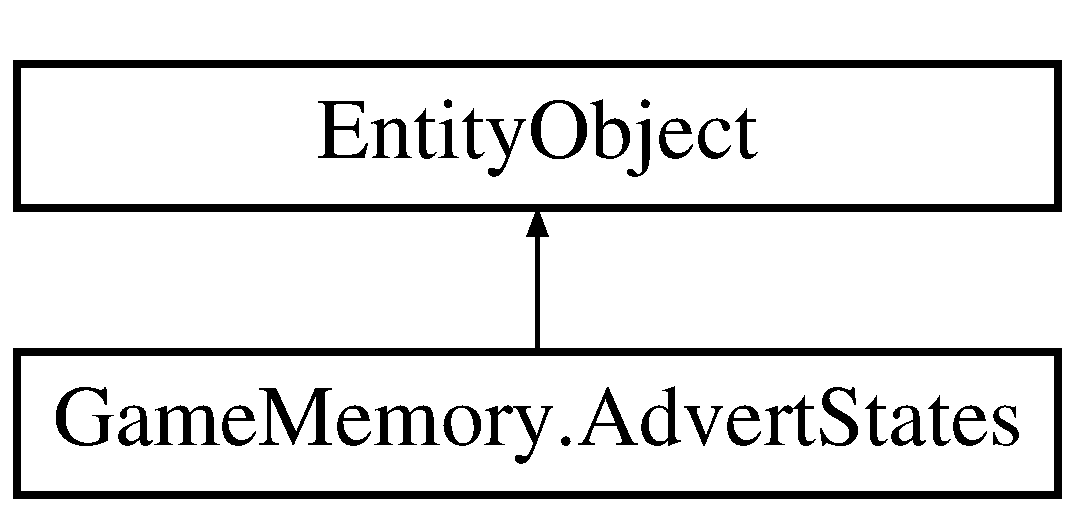
\includegraphics[height=2.000000cm]{class_game_memory_1_1_advert_states}
\end{center}
\end{figure}
\subsection*{Static Public Member Functions}
\begin{DoxyCompactItemize}
\item 
static \hyperlink{class_game_memory_1_1_advert_states}{Advert\-States} \hyperlink{class_game_memory_1_1_advert_states_ab0f190c459d819abb2ac6f270e94e124}{Create\-Advert\-States} (global\-::\-System.\-Int32 advertstate\-Id)
\begin{DoxyCompactList}\small\item\em Crear un nuevo objeto \hyperlink{class_game_memory_1_1_advert_states}{Advert\-States}. \end{DoxyCompactList}\end{DoxyCompactItemize}
\subsection*{Properties}
\begin{DoxyCompactItemize}
\item 
global\-::\-System.\-Int32 \hyperlink{class_game_memory_1_1_advert_states_a4fc6f03f0b82dcc6f7bec119f78ac16c}{Advertstate\-Id}\hspace{0.3cm}{\ttfamily  \mbox{[}get, set\mbox{]}}
\begin{DoxyCompactList}\small\item\em No hay documentación de metadatos disponible. \end{DoxyCompactList}\item 
global\-::\-System.\-String \hyperlink{class_game_memory_1_1_advert_states_af1d9170e4f56ed8db771b2f28bfa3307}{Description}\hspace{0.3cm}{\ttfamily  \mbox{[}get, set\mbox{]}}
\begin{DoxyCompactList}\small\item\em No hay documentación de metadatos disponible. \end{DoxyCompactList}\item 
Entity\-Collection$<$ \hyperlink{class_game_memory_1_1_adverts}{Adverts} $>$ \hyperlink{class_game_memory_1_1_advert_states_a67a482fee6ab0b3af3e41c91b33f263c}{Adverts}\hspace{0.3cm}{\ttfamily  \mbox{[}get, set\mbox{]}}
\begin{DoxyCompactList}\small\item\em No hay documentación de metadatos disponible. \end{DoxyCompactList}\end{DoxyCompactItemize}


\subsection{Detailed Description}
No hay documentación de metadatos disponible. 



\subsection{Member Function Documentation}
\hypertarget{class_game_memory_1_1_advert_states_ab0f190c459d819abb2ac6f270e94e124}{\index{Game\-Memory\-::\-Advert\-States@{Game\-Memory\-::\-Advert\-States}!Create\-Advert\-States@{Create\-Advert\-States}}
\index{Create\-Advert\-States@{Create\-Advert\-States}!GameMemory::AdvertStates@{Game\-Memory\-::\-Advert\-States}}
\subsubsection[{Create\-Advert\-States}]{\setlength{\rightskip}{0pt plus 5cm}static {\bf Advert\-States} Game\-Memory.\-Advert\-States.\-Create\-Advert\-States (
\begin{DoxyParamCaption}
\item[{global\-::\-System.\-Int32}]{advertstate\-Id}
\end{DoxyParamCaption}
)\hspace{0.3cm}{\ttfamily [static]}}}\label{class_game_memory_1_1_advert_states_ab0f190c459d819abb2ac6f270e94e124}


Crear un nuevo objeto \hyperlink{class_game_memory_1_1_advert_states}{Advert\-States}. 


\begin{DoxyParams}{Parameters}
{\em advertstate\-Id} & Valor inicial de la propiedad Advertstate\-Id.\\
\hline
\end{DoxyParams}


\subsection{Property Documentation}
\hypertarget{class_game_memory_1_1_advert_states_a67a482fee6ab0b3af3e41c91b33f263c}{\index{Game\-Memory\-::\-Advert\-States@{Game\-Memory\-::\-Advert\-States}!Adverts@{Adverts}}
\index{Adverts@{Adverts}!GameMemory::AdvertStates@{Game\-Memory\-::\-Advert\-States}}
\subsubsection[{Adverts}]{\setlength{\rightskip}{0pt plus 5cm}Entity\-Collection$<${\bf Adverts}$>$ Game\-Memory.\-Advert\-States.\-Adverts\hspace{0.3cm}{\ttfamily [get]}, {\ttfamily [set]}}}\label{class_game_memory_1_1_advert_states_a67a482fee6ab0b3af3e41c91b33f263c}


No hay documentación de metadatos disponible. 

\hypertarget{class_game_memory_1_1_advert_states_a4fc6f03f0b82dcc6f7bec119f78ac16c}{\index{Game\-Memory\-::\-Advert\-States@{Game\-Memory\-::\-Advert\-States}!Advertstate\-Id@{Advertstate\-Id}}
\index{Advertstate\-Id@{Advertstate\-Id}!GameMemory::AdvertStates@{Game\-Memory\-::\-Advert\-States}}
\subsubsection[{Advertstate\-Id}]{\setlength{\rightskip}{0pt plus 5cm}global.\-System.\-Int32 Game\-Memory.\-Advert\-States.\-Advertstate\-Id\hspace{0.3cm}{\ttfamily [get]}, {\ttfamily [set]}}}\label{class_game_memory_1_1_advert_states_a4fc6f03f0b82dcc6f7bec119f78ac16c}


No hay documentación de metadatos disponible. 

\hypertarget{class_game_memory_1_1_advert_states_af1d9170e4f56ed8db771b2f28bfa3307}{\index{Game\-Memory\-::\-Advert\-States@{Game\-Memory\-::\-Advert\-States}!Description@{Description}}
\index{Description@{Description}!GameMemory::AdvertStates@{Game\-Memory\-::\-Advert\-States}}
\subsubsection[{Description}]{\setlength{\rightskip}{0pt plus 5cm}global.\-System.\-String Game\-Memory.\-Advert\-States.\-Description\hspace{0.3cm}{\ttfamily [get]}, {\ttfamily [set]}}}\label{class_game_memory_1_1_advert_states_af1d9170e4f56ed8db771b2f28bfa3307}


No hay documentación de metadatos disponible. 



The documentation for this class was generated from the following file\-:\begin{DoxyCompactItemize}
\item 
D\-:/tesis\-Assembla/branches/\-Branch\-\_\-\-Tesis\-\_\-\-Sprint01/\-Dev/\-Interaction Module/\-Game\-Memory/\-Game\-Memory/O\-M\-K\-T.\-Designer.\-cs\end{DoxyCompactItemize}

\hypertarget{class_game_memory_1_1_advert_types}{\section{Game\-Memory.\-Advert\-Types Class Reference}
\label{class_game_memory_1_1_advert_types}\index{Game\-Memory.\-Advert\-Types@{Game\-Memory.\-Advert\-Types}}
}


No hay documentación de metadatos disponible.  


Inheritance diagram for Game\-Memory.\-Advert\-Types\-:\begin{figure}[H]
\begin{center}
\leavevmode
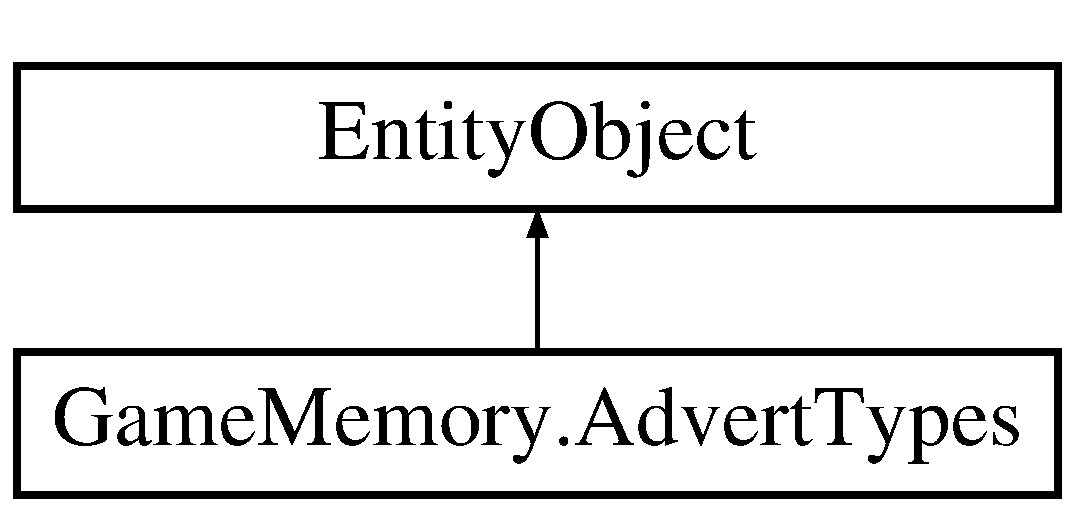
\includegraphics[height=2.000000cm]{class_game_memory_1_1_advert_types}
\end{center}
\end{figure}
\subsection*{Static Public Member Functions}
\begin{DoxyCompactItemize}
\item 
static \hyperlink{class_game_memory_1_1_advert_types}{Advert\-Types} \hyperlink{class_game_memory_1_1_advert_types_a55bb5ec594393be2d7b4c47ae3282cb0}{Create\-Advert\-Types} (global\-::\-System.\-Int32 advert\-Type\-Id)
\begin{DoxyCompactList}\small\item\em Crear un nuevo objeto \hyperlink{class_game_memory_1_1_advert_types}{Advert\-Types}. \end{DoxyCompactList}\end{DoxyCompactItemize}
\subsection*{Properties}
\begin{DoxyCompactItemize}
\item 
global\-::\-System.\-Int32 \hyperlink{class_game_memory_1_1_advert_types_ac21bad53ca69cb06497c450799dbeb43}{Advert\-Type\-Id}\hspace{0.3cm}{\ttfamily  \mbox{[}get, set\mbox{]}}
\begin{DoxyCompactList}\small\item\em No hay documentación de metadatos disponible. \end{DoxyCompactList}\item 
global\-::\-System.\-String \hyperlink{class_game_memory_1_1_advert_types_af676476a49a59ae0784817869e6f0a26}{Description}\hspace{0.3cm}{\ttfamily  \mbox{[}get, set\mbox{]}}
\begin{DoxyCompactList}\small\item\em No hay documentación de metadatos disponible. \end{DoxyCompactList}\item 
Entity\-Collection$<$ \hyperlink{class_game_memory_1_1_adverts}{Adverts} $>$ \hyperlink{class_game_memory_1_1_advert_types_a36bf93fbe09421a21be95837059d0211}{Adverts}\hspace{0.3cm}{\ttfamily  \mbox{[}get, set\mbox{]}}
\begin{DoxyCompactList}\small\item\em No hay documentación de metadatos disponible. \end{DoxyCompactList}\end{DoxyCompactItemize}


\subsection{Detailed Description}
No hay documentación de metadatos disponible. 



\subsection{Member Function Documentation}
\hypertarget{class_game_memory_1_1_advert_types_a55bb5ec594393be2d7b4c47ae3282cb0}{\index{Game\-Memory\-::\-Advert\-Types@{Game\-Memory\-::\-Advert\-Types}!Create\-Advert\-Types@{Create\-Advert\-Types}}
\index{Create\-Advert\-Types@{Create\-Advert\-Types}!GameMemory::AdvertTypes@{Game\-Memory\-::\-Advert\-Types}}
\subsubsection[{Create\-Advert\-Types}]{\setlength{\rightskip}{0pt plus 5cm}static {\bf Advert\-Types} Game\-Memory.\-Advert\-Types.\-Create\-Advert\-Types (
\begin{DoxyParamCaption}
\item[{global\-::\-System.\-Int32}]{advert\-Type\-Id}
\end{DoxyParamCaption}
)\hspace{0.3cm}{\ttfamily [static]}}}\label{class_game_memory_1_1_advert_types_a55bb5ec594393be2d7b4c47ae3282cb0}


Crear un nuevo objeto \hyperlink{class_game_memory_1_1_advert_types}{Advert\-Types}. 


\begin{DoxyParams}{Parameters}
{\em advert\-Type\-Id} & Valor inicial de la propiedad Advert\-Type\-Id.\\
\hline
\end{DoxyParams}


\subsection{Property Documentation}
\hypertarget{class_game_memory_1_1_advert_types_a36bf93fbe09421a21be95837059d0211}{\index{Game\-Memory\-::\-Advert\-Types@{Game\-Memory\-::\-Advert\-Types}!Adverts@{Adverts}}
\index{Adverts@{Adverts}!GameMemory::AdvertTypes@{Game\-Memory\-::\-Advert\-Types}}
\subsubsection[{Adverts}]{\setlength{\rightskip}{0pt plus 5cm}Entity\-Collection$<${\bf Adverts}$>$ Game\-Memory.\-Advert\-Types.\-Adverts\hspace{0.3cm}{\ttfamily [get]}, {\ttfamily [set]}}}\label{class_game_memory_1_1_advert_types_a36bf93fbe09421a21be95837059d0211}


No hay documentación de metadatos disponible. 

\hypertarget{class_game_memory_1_1_advert_types_ac21bad53ca69cb06497c450799dbeb43}{\index{Game\-Memory\-::\-Advert\-Types@{Game\-Memory\-::\-Advert\-Types}!Advert\-Type\-Id@{Advert\-Type\-Id}}
\index{Advert\-Type\-Id@{Advert\-Type\-Id}!GameMemory::AdvertTypes@{Game\-Memory\-::\-Advert\-Types}}
\subsubsection[{Advert\-Type\-Id}]{\setlength{\rightskip}{0pt plus 5cm}global.\-System.\-Int32 Game\-Memory.\-Advert\-Types.\-Advert\-Type\-Id\hspace{0.3cm}{\ttfamily [get]}, {\ttfamily [set]}}}\label{class_game_memory_1_1_advert_types_ac21bad53ca69cb06497c450799dbeb43}


No hay documentación de metadatos disponible. 

\hypertarget{class_game_memory_1_1_advert_types_af676476a49a59ae0784817869e6f0a26}{\index{Game\-Memory\-::\-Advert\-Types@{Game\-Memory\-::\-Advert\-Types}!Description@{Description}}
\index{Description@{Description}!GameMemory::AdvertTypes@{Game\-Memory\-::\-Advert\-Types}}
\subsubsection[{Description}]{\setlength{\rightskip}{0pt plus 5cm}global.\-System.\-String Game\-Memory.\-Advert\-Types.\-Description\hspace{0.3cm}{\ttfamily [get]}, {\ttfamily [set]}}}\label{class_game_memory_1_1_advert_types_af676476a49a59ae0784817869e6f0a26}


No hay documentación de metadatos disponible. 



The documentation for this class was generated from the following file\-:\begin{DoxyCompactItemize}
\item 
D\-:/tesis\-Assembla/branches/\-Branch\-\_\-\-Tesis\-\_\-\-Sprint01/\-Dev/\-Interaction Module/\-Game\-Memory/\-Game\-Memory/O\-M\-K\-T.\-Designer.\-cs\end{DoxyCompactItemize}

\hypertarget{class_game_memory_1_1_advert_video}{\section{Game\-Memory.\-Advert\-Video Class Reference}
\label{class_game_memory_1_1_advert_video}\index{Game\-Memory.\-Advert\-Video@{Game\-Memory.\-Advert\-Video}}
}


\hyperlink{class_game_memory_1_1_advert_video}{Advert\-Video}  


Inheritance diagram for Game\-Memory.\-Advert\-Video\-:\begin{figure}[H]
\begin{center}
\leavevmode
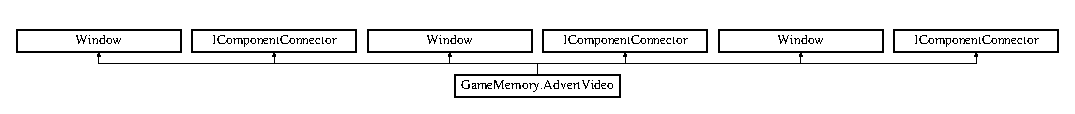
\includegraphics[height=1.078998cm]{class_game_memory_1_1_advert_video}
\end{center}
\end{figure}
\subsection*{Public Member Functions}
\begin{DoxyCompactItemize}
\item 
void \hyperlink{class_game_memory_1_1_advert_video_ac7bf62d252772c82159d8c597ced23f8}{Initialize\-Component} ()
\begin{DoxyCompactList}\small\item\em Initialize\-Component \end{DoxyCompactList}\item 
void \hyperlink{class_game_memory_1_1_advert_video_ac7bf62d252772c82159d8c597ced23f8}{Initialize\-Component} ()
\begin{DoxyCompactList}\small\item\em Initialize\-Component \end{DoxyCompactList}\item 
void \hyperlink{class_game_memory_1_1_advert_video_ac7bf62d252772c82159d8c597ced23f8}{Initialize\-Component} ()
\begin{DoxyCompactList}\small\item\em Initialize\-Component \end{DoxyCompactList}\end{DoxyCompactItemize}


\subsection{Detailed Description}
\hyperlink{class_game_memory_1_1_advert_video}{Advert\-Video} 

Class Ventana que reproduce videos publicitarios.

\subsection{Member Function Documentation}
\hypertarget{class_game_memory_1_1_advert_video_ac7bf62d252772c82159d8c597ced23f8}{\index{Game\-Memory\-::\-Advert\-Video@{Game\-Memory\-::\-Advert\-Video}!Initialize\-Component@{Initialize\-Component}}
\index{Initialize\-Component@{Initialize\-Component}!GameMemory::AdvertVideo@{Game\-Memory\-::\-Advert\-Video}}
\subsubsection[{Initialize\-Component}]{\setlength{\rightskip}{0pt plus 5cm}void Game\-Memory.\-Advert\-Video.\-Initialize\-Component (
\begin{DoxyParamCaption}
{}
\end{DoxyParamCaption}
)}}\label{class_game_memory_1_1_advert_video_ac7bf62d252772c82159d8c597ced23f8}


Initialize\-Component 

\hypertarget{class_game_memory_1_1_advert_video_ac7bf62d252772c82159d8c597ced23f8}{\index{Game\-Memory\-::\-Advert\-Video@{Game\-Memory\-::\-Advert\-Video}!Initialize\-Component@{Initialize\-Component}}
\index{Initialize\-Component@{Initialize\-Component}!GameMemory::AdvertVideo@{Game\-Memory\-::\-Advert\-Video}}
\subsubsection[{Initialize\-Component}]{\setlength{\rightskip}{0pt plus 5cm}void Game\-Memory.\-Advert\-Video.\-Initialize\-Component (
\begin{DoxyParamCaption}
{}
\end{DoxyParamCaption}
)}}\label{class_game_memory_1_1_advert_video_ac7bf62d252772c82159d8c597ced23f8}


Initialize\-Component 

\hypertarget{class_game_memory_1_1_advert_video_ac7bf62d252772c82159d8c597ced23f8}{\index{Game\-Memory\-::\-Advert\-Video@{Game\-Memory\-::\-Advert\-Video}!Initialize\-Component@{Initialize\-Component}}
\index{Initialize\-Component@{Initialize\-Component}!GameMemory::AdvertVideo@{Game\-Memory\-::\-Advert\-Video}}
\subsubsection[{Initialize\-Component}]{\setlength{\rightskip}{0pt plus 5cm}void Game\-Memory.\-Advert\-Video.\-Initialize\-Component (
\begin{DoxyParamCaption}
{}
\end{DoxyParamCaption}
)}}\label{class_game_memory_1_1_advert_video_ac7bf62d252772c82159d8c597ced23f8}


Initialize\-Component 



The documentation for this class was generated from the following files\-:\begin{DoxyCompactItemize}
\item 
D\-:/tesis\-Assembla/branches/\-Branch\-\_\-\-Tesis\-\_\-\-Sprint01/\-Dev/\-Interaction Module/\-Game\-Memory/\-Game\-Memory/advert\-Video.\-xaml.\-cs\item 
D\-:/tesis\-Assembla/branches/\-Branch\-\_\-\-Tesis\-\_\-\-Sprint01/\-Dev/\-Interaction Module/\-Game\-Memory/\-Game\-Memory/obj/x86/\-Debug/advert\-Video.\-g.\-cs\item 
D\-:/tesis\-Assembla/branches/\-Branch\-\_\-\-Tesis\-\_\-\-Sprint01/\-Dev/\-Interaction Module/\-Game\-Memory/\-Game\-Memory/obj/x86/\-Debug/advert\-Video.\-g.\-i.\-cs\item 
D\-:/tesis\-Assembla/branches/\-Branch\-\_\-\-Tesis\-\_\-\-Sprint01/\-Dev/\-Interaction Module/\-Game\-Memory/\-Game\-Memory/obj/x86/\-Release/advert\-Video.\-g.\-i.\-cs\end{DoxyCompactItemize}

\hypertarget{class_game_memory_1_1_alerts}{\section{Game\-Memory.\-Alerts Class Reference}
\label{class_game_memory_1_1_alerts}\index{Game\-Memory.\-Alerts@{Game\-Memory.\-Alerts}}
}


No hay documentación de metadatos disponible.  


Inheritance diagram for Game\-Memory.\-Alerts\-:\begin{figure}[H]
\begin{center}
\leavevmode
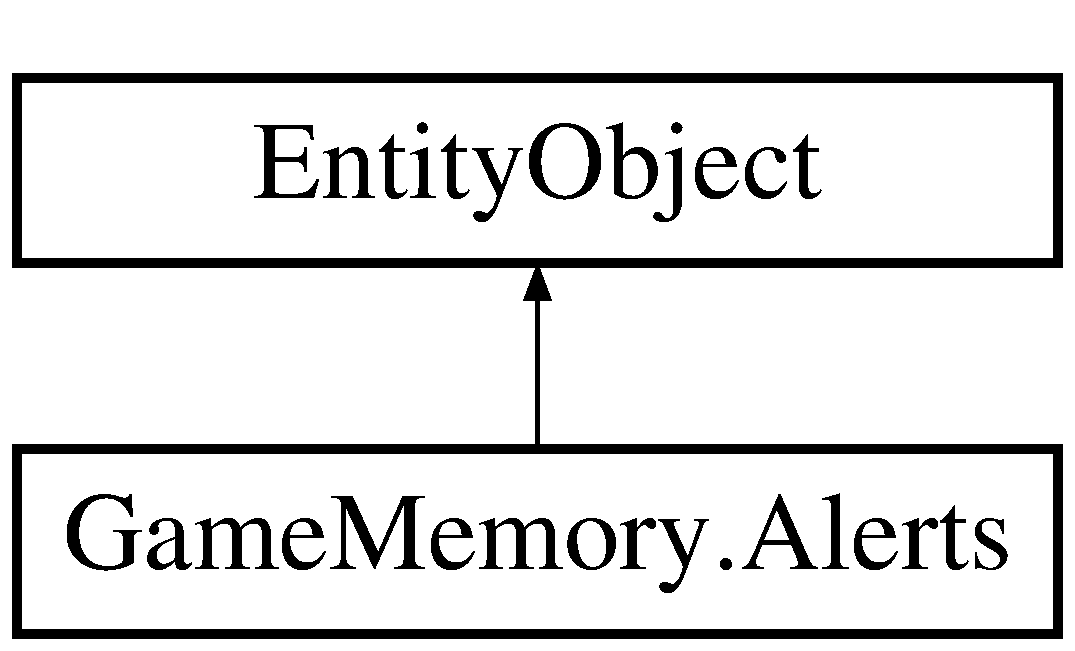
\includegraphics[height=2.000000cm]{class_game_memory_1_1_alerts}
\end{center}
\end{figure}
\subsection*{Static Public Member Functions}
\begin{DoxyCompactItemize}
\item 
static \hyperlink{class_game_memory_1_1_alerts}{Alerts} \hyperlink{class_game_memory_1_1_alerts_a0ded6ee29a08738d78ef75d91c160920}{Create\-Alerts} (global\-::\-System.\-Int32 alert\-Id, global\-::\-System.\-Int32 customer\-Id)
\begin{DoxyCompactList}\small\item\em Crear un nuevo objeto \hyperlink{class_game_memory_1_1_alerts}{Alerts}. \end{DoxyCompactList}\end{DoxyCompactItemize}
\subsection*{Properties}
\begin{DoxyCompactItemize}
\item 
global\-::\-System.\-Int32 \hyperlink{class_game_memory_1_1_alerts_a6e1cbcb967beb6bf83452ffa6be8b679}{Alert\-Id}\hspace{0.3cm}{\ttfamily  \mbox{[}get, set\mbox{]}}
\begin{DoxyCompactList}\small\item\em No hay documentación de metadatos disponible. \end{DoxyCompactList}\item 
global\-::\-System.\-String \hyperlink{class_game_memory_1_1_alerts_a52f59bb44b174d6c60521a9d226a4cf8}{Message}\hspace{0.3cm}{\ttfamily  \mbox{[}get, set\mbox{]}}
\begin{DoxyCompactList}\small\item\em No hay documentación de metadatos disponible. \end{DoxyCompactList}\item 
Nullable$<$ global\-::\-System.\-Date\-Time $>$ \hyperlink{class_game_memory_1_1_alerts_a9f7acf9c7a5e7248df9a8c2c2f841ca9}{Date}\hspace{0.3cm}{\ttfamily  \mbox{[}get, set\mbox{]}}
\begin{DoxyCompactList}\small\item\em No hay documentación de metadatos disponible. \end{DoxyCompactList}\item 
global\-::\-System.\-Int32 \hyperlink{class_game_memory_1_1_alerts_a65ef174df77f25f7e1725f53b38ba3a9}{Customer\-Id}\hspace{0.3cm}{\ttfamily  \mbox{[}get, set\mbox{]}}
\begin{DoxyCompactList}\small\item\em No hay documentación de metadatos disponible. \end{DoxyCompactList}\item 
\hyperlink{class_game_memory_1_1_customers}{Customers} \hyperlink{class_game_memory_1_1_alerts_a95f4e83172bc78c6d100de58837b5949}{Customers}\hspace{0.3cm}{\ttfamily  \mbox{[}get, set\mbox{]}}
\begin{DoxyCompactList}\small\item\em No hay documentación de metadatos disponible. \end{DoxyCompactList}\item 
Entity\-Reference$<$ \hyperlink{class_game_memory_1_1_customers}{Customers} $>$ \hyperlink{class_game_memory_1_1_alerts_a413ffe3f68f3c9e23cef4d542106fd97}{Customers\-Reference}\hspace{0.3cm}{\ttfamily  \mbox{[}get, set\mbox{]}}
\begin{DoxyCompactList}\small\item\em No hay documentación de metadatos disponible. \end{DoxyCompactList}\end{DoxyCompactItemize}


\subsection{Detailed Description}
No hay documentación de metadatos disponible. 



\subsection{Member Function Documentation}
\hypertarget{class_game_memory_1_1_alerts_a0ded6ee29a08738d78ef75d91c160920}{\index{Game\-Memory\-::\-Alerts@{Game\-Memory\-::\-Alerts}!Create\-Alerts@{Create\-Alerts}}
\index{Create\-Alerts@{Create\-Alerts}!GameMemory::Alerts@{Game\-Memory\-::\-Alerts}}
\subsubsection[{Create\-Alerts}]{\setlength{\rightskip}{0pt plus 5cm}static {\bf Alerts} Game\-Memory.\-Alerts.\-Create\-Alerts (
\begin{DoxyParamCaption}
\item[{global\-::\-System.\-Int32}]{alert\-Id, }
\item[{global\-::\-System.\-Int32}]{customer\-Id}
\end{DoxyParamCaption}
)\hspace{0.3cm}{\ttfamily [static]}}}\label{class_game_memory_1_1_alerts_a0ded6ee29a08738d78ef75d91c160920}


Crear un nuevo objeto \hyperlink{class_game_memory_1_1_alerts}{Alerts}. 


\begin{DoxyParams}{Parameters}
{\em alert\-Id} & Valor inicial de la propiedad Alert\-Id.\\
\hline
{\em customer\-Id} & Valor inicial de la propiedad Customer\-Id.\\
\hline
\end{DoxyParams}


\subsection{Property Documentation}
\hypertarget{class_game_memory_1_1_alerts_a6e1cbcb967beb6bf83452ffa6be8b679}{\index{Game\-Memory\-::\-Alerts@{Game\-Memory\-::\-Alerts}!Alert\-Id@{Alert\-Id}}
\index{Alert\-Id@{Alert\-Id}!GameMemory::Alerts@{Game\-Memory\-::\-Alerts}}
\subsubsection[{Alert\-Id}]{\setlength{\rightskip}{0pt plus 5cm}global.\-System.\-Int32 Game\-Memory.\-Alerts.\-Alert\-Id\hspace{0.3cm}{\ttfamily [get]}, {\ttfamily [set]}}}\label{class_game_memory_1_1_alerts_a6e1cbcb967beb6bf83452ffa6be8b679}


No hay documentación de metadatos disponible. 

\hypertarget{class_game_memory_1_1_alerts_a65ef174df77f25f7e1725f53b38ba3a9}{\index{Game\-Memory\-::\-Alerts@{Game\-Memory\-::\-Alerts}!Customer\-Id@{Customer\-Id}}
\index{Customer\-Id@{Customer\-Id}!GameMemory::Alerts@{Game\-Memory\-::\-Alerts}}
\subsubsection[{Customer\-Id}]{\setlength{\rightskip}{0pt plus 5cm}global.\-System.\-Int32 Game\-Memory.\-Alerts.\-Customer\-Id\hspace{0.3cm}{\ttfamily [get]}, {\ttfamily [set]}}}\label{class_game_memory_1_1_alerts_a65ef174df77f25f7e1725f53b38ba3a9}


No hay documentación de metadatos disponible. 

\hypertarget{class_game_memory_1_1_alerts_a95f4e83172bc78c6d100de58837b5949}{\index{Game\-Memory\-::\-Alerts@{Game\-Memory\-::\-Alerts}!Customers@{Customers}}
\index{Customers@{Customers}!GameMemory::Alerts@{Game\-Memory\-::\-Alerts}}
\subsubsection[{Customers}]{\setlength{\rightskip}{0pt plus 5cm}{\bf Customers} Game\-Memory.\-Alerts.\-Customers\hspace{0.3cm}{\ttfamily [get]}, {\ttfamily [set]}}}\label{class_game_memory_1_1_alerts_a95f4e83172bc78c6d100de58837b5949}


No hay documentación de metadatos disponible. 

\hypertarget{class_game_memory_1_1_alerts_a413ffe3f68f3c9e23cef4d542106fd97}{\index{Game\-Memory\-::\-Alerts@{Game\-Memory\-::\-Alerts}!Customers\-Reference@{Customers\-Reference}}
\index{Customers\-Reference@{Customers\-Reference}!GameMemory::Alerts@{Game\-Memory\-::\-Alerts}}
\subsubsection[{Customers\-Reference}]{\setlength{\rightskip}{0pt plus 5cm}Entity\-Reference$<${\bf Customers}$>$ Game\-Memory.\-Alerts.\-Customers\-Reference\hspace{0.3cm}{\ttfamily [get]}, {\ttfamily [set]}}}\label{class_game_memory_1_1_alerts_a413ffe3f68f3c9e23cef4d542106fd97}


No hay documentación de metadatos disponible. 

\hypertarget{class_game_memory_1_1_alerts_a9f7acf9c7a5e7248df9a8c2c2f841ca9}{\index{Game\-Memory\-::\-Alerts@{Game\-Memory\-::\-Alerts}!Date@{Date}}
\index{Date@{Date}!GameMemory::Alerts@{Game\-Memory\-::\-Alerts}}
\subsubsection[{Date}]{\setlength{\rightskip}{0pt plus 5cm}Nullable$<$global.\-System.\-Date\-Time$>$ Game\-Memory.\-Alerts.\-Date\hspace{0.3cm}{\ttfamily [get]}, {\ttfamily [set]}}}\label{class_game_memory_1_1_alerts_a9f7acf9c7a5e7248df9a8c2c2f841ca9}


No hay documentación de metadatos disponible. 

\hypertarget{class_game_memory_1_1_alerts_a52f59bb44b174d6c60521a9d226a4cf8}{\index{Game\-Memory\-::\-Alerts@{Game\-Memory\-::\-Alerts}!Message@{Message}}
\index{Message@{Message}!GameMemory::Alerts@{Game\-Memory\-::\-Alerts}}
\subsubsection[{Message}]{\setlength{\rightskip}{0pt plus 5cm}global.\-System.\-String Game\-Memory.\-Alerts.\-Message\hspace{0.3cm}{\ttfamily [get]}, {\ttfamily [set]}}}\label{class_game_memory_1_1_alerts_a52f59bb44b174d6c60521a9d226a4cf8}


No hay documentación de metadatos disponible. 



The documentation for this class was generated from the following file\-:\begin{DoxyCompactItemize}
\item 
D\-:/tesis\-Assembla/branches/\-Branch\-\_\-\-Tesis\-\_\-\-Sprint01/\-Dev/\-Interaction Module/\-Game\-Memory/\-Game\-Memory/O\-M\-K\-T.\-Designer.\-cs\end{DoxyCompactItemize}

\hypertarget{class_game_memory_1_1_app}{\section{Game\-Memory.\-App Class Reference}
\label{class_game_memory_1_1_app}\index{Game\-Memory.\-App@{Game\-Memory.\-App}}
}


Lógica de interacción para App.\-xaml  


Inheritance diagram for Game\-Memory.\-App\-:\begin{figure}[H]
\begin{center}
\leavevmode
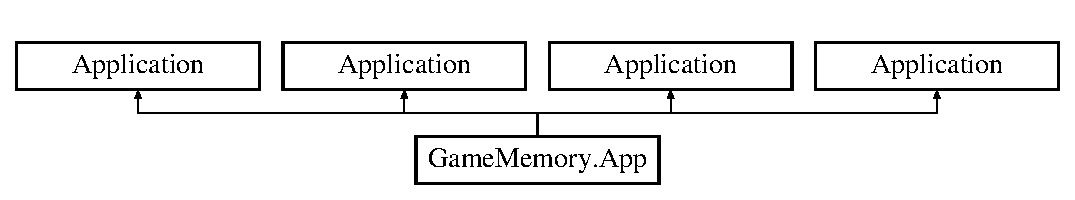
\includegraphics[height=2.000000cm]{class_game_memory_1_1_app}
\end{center}
\end{figure}
\subsection*{Public Member Functions}
\begin{DoxyCompactItemize}
\item 
void \hyperlink{class_game_memory_1_1_app_a8cd0811afa0643c63fdf78ec2450ec10}{Initialize\-Component} ()
\begin{DoxyCompactList}\small\item\em Initialize\-Component \end{DoxyCompactList}\item 
void \hyperlink{class_game_memory_1_1_app_a8cd0811afa0643c63fdf78ec2450ec10}{Initialize\-Component} ()
\begin{DoxyCompactList}\small\item\em Initialize\-Component \end{DoxyCompactList}\item 
void \hyperlink{class_game_memory_1_1_app_a8cd0811afa0643c63fdf78ec2450ec10}{Initialize\-Component} ()
\begin{DoxyCompactList}\small\item\em Initialize\-Component \end{DoxyCompactList}\end{DoxyCompactItemize}
\subsection*{Static Public Member Functions}
\begin{DoxyCompactItemize}
\item 
static void \hyperlink{class_game_memory_1_1_app_a3e19978683fa23b7f5d517ca4fada97d}{Main} ()
\begin{DoxyCompactList}\small\item\em Application Entry Point. \end{DoxyCompactList}\item 
static void \hyperlink{class_game_memory_1_1_app_a3e19978683fa23b7f5d517ca4fada97d}{Main} ()
\begin{DoxyCompactList}\small\item\em Application Entry Point. \end{DoxyCompactList}\item 
static void \hyperlink{class_game_memory_1_1_app_a3e19978683fa23b7f5d517ca4fada97d}{Main} ()
\begin{DoxyCompactList}\small\item\em Application Entry Point. \end{DoxyCompactList}\end{DoxyCompactItemize}


\subsection{Detailed Description}
Lógica de interacción para App.\-xaml 

\hyperlink{class_game_memory_1_1_app}{App} 

\subsection{Member Function Documentation}
\hypertarget{class_game_memory_1_1_app_a8cd0811afa0643c63fdf78ec2450ec10}{\index{Game\-Memory\-::\-App@{Game\-Memory\-::\-App}!Initialize\-Component@{Initialize\-Component}}
\index{Initialize\-Component@{Initialize\-Component}!GameMemory::App@{Game\-Memory\-::\-App}}
\subsubsection[{Initialize\-Component}]{\setlength{\rightskip}{0pt plus 5cm}void Game\-Memory.\-App.\-Initialize\-Component (
\begin{DoxyParamCaption}
{}
\end{DoxyParamCaption}
)}}\label{class_game_memory_1_1_app_a8cd0811afa0643c63fdf78ec2450ec10}


Initialize\-Component 

\hypertarget{class_game_memory_1_1_app_a8cd0811afa0643c63fdf78ec2450ec10}{\index{Game\-Memory\-::\-App@{Game\-Memory\-::\-App}!Initialize\-Component@{Initialize\-Component}}
\index{Initialize\-Component@{Initialize\-Component}!GameMemory::App@{Game\-Memory\-::\-App}}
\subsubsection[{Initialize\-Component}]{\setlength{\rightskip}{0pt plus 5cm}void Game\-Memory.\-App.\-Initialize\-Component (
\begin{DoxyParamCaption}
{}
\end{DoxyParamCaption}
)}}\label{class_game_memory_1_1_app_a8cd0811afa0643c63fdf78ec2450ec10}


Initialize\-Component 

\hypertarget{class_game_memory_1_1_app_a8cd0811afa0643c63fdf78ec2450ec10}{\index{Game\-Memory\-::\-App@{Game\-Memory\-::\-App}!Initialize\-Component@{Initialize\-Component}}
\index{Initialize\-Component@{Initialize\-Component}!GameMemory::App@{Game\-Memory\-::\-App}}
\subsubsection[{Initialize\-Component}]{\setlength{\rightskip}{0pt plus 5cm}void Game\-Memory.\-App.\-Initialize\-Component (
\begin{DoxyParamCaption}
{}
\end{DoxyParamCaption}
)}}\label{class_game_memory_1_1_app_a8cd0811afa0643c63fdf78ec2450ec10}


Initialize\-Component 

\hypertarget{class_game_memory_1_1_app_a3e19978683fa23b7f5d517ca4fada97d}{\index{Game\-Memory\-::\-App@{Game\-Memory\-::\-App}!Main@{Main}}
\index{Main@{Main}!GameMemory::App@{Game\-Memory\-::\-App}}
\subsubsection[{Main}]{\setlength{\rightskip}{0pt plus 5cm}static void Game\-Memory.\-App.\-Main (
\begin{DoxyParamCaption}
{}
\end{DoxyParamCaption}
)\hspace{0.3cm}{\ttfamily [static]}}}\label{class_game_memory_1_1_app_a3e19978683fa23b7f5d517ca4fada97d}


Application Entry Point. 

\hypertarget{class_game_memory_1_1_app_a3e19978683fa23b7f5d517ca4fada97d}{\index{Game\-Memory\-::\-App@{Game\-Memory\-::\-App}!Main@{Main}}
\index{Main@{Main}!GameMemory::App@{Game\-Memory\-::\-App}}
\subsubsection[{Main}]{\setlength{\rightskip}{0pt plus 5cm}static void Game\-Memory.\-App.\-Main (
\begin{DoxyParamCaption}
{}
\end{DoxyParamCaption}
)\hspace{0.3cm}{\ttfamily [static]}}}\label{class_game_memory_1_1_app_a3e19978683fa23b7f5d517ca4fada97d}


Application Entry Point. 

\hypertarget{class_game_memory_1_1_app_a3e19978683fa23b7f5d517ca4fada97d}{\index{Game\-Memory\-::\-App@{Game\-Memory\-::\-App}!Main@{Main}}
\index{Main@{Main}!GameMemory::App@{Game\-Memory\-::\-App}}
\subsubsection[{Main}]{\setlength{\rightskip}{0pt plus 5cm}static void Game\-Memory.\-App.\-Main (
\begin{DoxyParamCaption}
{}
\end{DoxyParamCaption}
)\hspace{0.3cm}{\ttfamily [static]}}}\label{class_game_memory_1_1_app_a3e19978683fa23b7f5d517ca4fada97d}


Application Entry Point. 



The documentation for this class was generated from the following files\-:\begin{DoxyCompactItemize}
\item 
D\-:/tesis\-Assembla/branches/\-Branch\-\_\-\-Tesis\-\_\-\-Sprint01/\-Dev/\-Interaction Module/\-Game\-Memory/\-Game\-Memory/App.\-xaml.\-cs\item 
D\-:/tesis\-Assembla/branches/\-Branch\-\_\-\-Tesis\-\_\-\-Sprint01/\-Dev/\-Interaction Module/\-Game\-Memory/\-Game\-Memory/obj/x86/\-Debug/App.\-g.\-cs\item 
D\-:/tesis\-Assembla/branches/\-Branch\-\_\-\-Tesis\-\_\-\-Sprint01/\-Dev/\-Interaction Module/\-Game\-Memory/\-Game\-Memory/obj/x86/\-Debug/App.\-g.\-i.\-cs\item 
D\-:/tesis\-Assembla/branches/\-Branch\-\_\-\-Tesis\-\_\-\-Sprint01/\-Dev/\-Interaction Module/\-Game\-Memory/\-Game\-Memory/obj/x86/\-Release/App.\-g.\-i.\-cs\end{DoxyCompactItemize}

\hypertarget{class_game_memory_1_1_c_____migration_history}{\section{Game\-Memory.\-C\-\_\-\-\_\-\-Migration\-History Class Reference}
\label{class_game_memory_1_1_c_____migration_history}\index{Game\-Memory.\-C\-\_\-\-\_\-\-Migration\-History@{Game\-Memory.\-C\-\_\-\-\_\-\-Migration\-History}}
}


No hay documentación de metadatos disponible.  


Inheritance diagram for Game\-Memory.\-C\-\_\-\-\_\-\-Migration\-History\-:\begin{figure}[H]
\begin{center}
\leavevmode
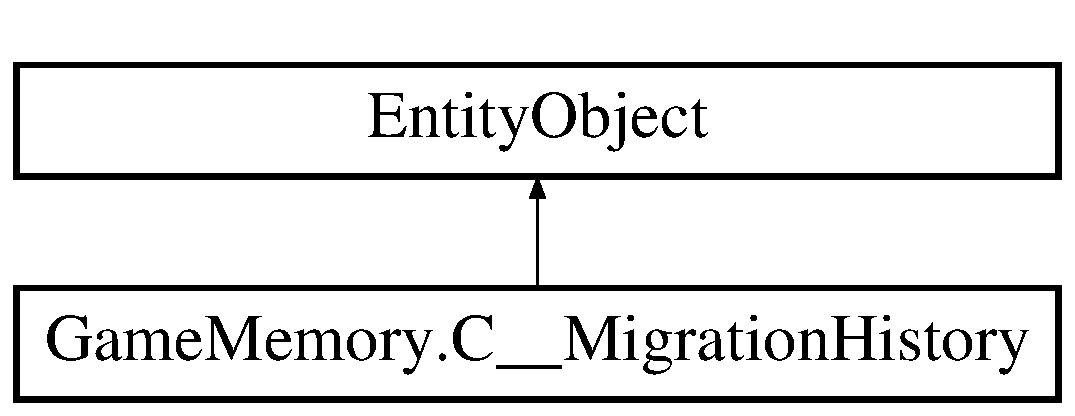
\includegraphics[height=2.000000cm]{class_game_memory_1_1_c_____migration_history}
\end{center}
\end{figure}
\subsection*{Static Public Member Functions}
\begin{DoxyCompactItemize}
\item 
static \hyperlink{class_game_memory_1_1_c_____migration_history}{C\-\_\-\-\_\-\-Migration\-History} \hyperlink{class_game_memory_1_1_c_____migration_history_a8c48f47af87e55bad0a9084d92b4b977}{Create\-C\-\_\-\-\_\-\-Migration\-History} (global\-::\-System.\-String migration\-Id, global\-::\-System.\-Byte\mbox{[}$\,$\mbox{]} model, global\-::\-System.\-String product\-Version)
\begin{DoxyCompactList}\small\item\em Crear un nuevo objeto \hyperlink{class_game_memory_1_1_c_____migration_history}{C\-\_\-\-\_\-\-Migration\-History}. \end{DoxyCompactList}\end{DoxyCompactItemize}
\subsection*{Properties}
\begin{DoxyCompactItemize}
\item 
global\-::\-System.\-String \hyperlink{class_game_memory_1_1_c_____migration_history_aa3b7056950a36d9f1beec90a885528d6}{Migration\-Id}\hspace{0.3cm}{\ttfamily  \mbox{[}get, set\mbox{]}}
\begin{DoxyCompactList}\small\item\em No hay documentación de metadatos disponible. \end{DoxyCompactList}\item 
global\-::\-System.\-Byte\mbox{[}$\,$\mbox{]} \hyperlink{class_game_memory_1_1_c_____migration_history_a58891e2fdcbaa080ac0552ececafc6e9}{Model}\hspace{0.3cm}{\ttfamily  \mbox{[}get, set\mbox{]}}
\begin{DoxyCompactList}\small\item\em No hay documentación de metadatos disponible. \end{DoxyCompactList}\item 
global\-::\-System.\-String \hyperlink{class_game_memory_1_1_c_____migration_history_a0ed9c308a2f2cb884bf4ed841e400093}{Product\-Version}\hspace{0.3cm}{\ttfamily  \mbox{[}get, set\mbox{]}}
\begin{DoxyCompactList}\small\item\em No hay documentación de metadatos disponible. \end{DoxyCompactList}\end{DoxyCompactItemize}


\subsection{Detailed Description}
No hay documentación de metadatos disponible. 



\subsection{Member Function Documentation}
\hypertarget{class_game_memory_1_1_c_____migration_history_a8c48f47af87e55bad0a9084d92b4b977}{\index{Game\-Memory\-::\-C\-\_\-\-\_\-\-Migration\-History@{Game\-Memory\-::\-C\-\_\-\-\_\-\-Migration\-History}!Create\-C\-\_\-\-\_\-\-Migration\-History@{Create\-C\-\_\-\-\_\-\-Migration\-History}}
\index{Create\-C\-\_\-\-\_\-\-Migration\-History@{Create\-C\-\_\-\-\_\-\-Migration\-History}!GameMemory::C__MigrationHistory@{Game\-Memory\-::\-C\-\_\-\-\_\-\-Migration\-History}}
\subsubsection[{Create\-C\-\_\-\-\_\-\-Migration\-History}]{\setlength{\rightskip}{0pt plus 5cm}static {\bf C\-\_\-\-\_\-\-Migration\-History} Game\-Memory.\-C\-\_\-\-\_\-\-Migration\-History.\-Create\-C\-\_\-\-\_\-\-Migration\-History (
\begin{DoxyParamCaption}
\item[{global\-::\-System.\-String}]{migration\-Id, }
\item[{global\-::\-System.\-Byte\mbox{[}$\,$\mbox{]}}]{model, }
\item[{global\-::\-System.\-String}]{product\-Version}
\end{DoxyParamCaption}
)\hspace{0.3cm}{\ttfamily [static]}}}\label{class_game_memory_1_1_c_____migration_history_a8c48f47af87e55bad0a9084d92b4b977}


Crear un nuevo objeto \hyperlink{class_game_memory_1_1_c_____migration_history}{C\-\_\-\-\_\-\-Migration\-History}. 


\begin{DoxyParams}{Parameters}
{\em migration\-Id} & Valor inicial de la propiedad Migration\-Id.\\
\hline
{\em model} & Valor inicial de la propiedad Model.\\
\hline
{\em product\-Version} & Valor inicial de la propiedad Product\-Version.\\
\hline
\end{DoxyParams}


\subsection{Property Documentation}
\hypertarget{class_game_memory_1_1_c_____migration_history_aa3b7056950a36d9f1beec90a885528d6}{\index{Game\-Memory\-::\-C\-\_\-\-\_\-\-Migration\-History@{Game\-Memory\-::\-C\-\_\-\-\_\-\-Migration\-History}!Migration\-Id@{Migration\-Id}}
\index{Migration\-Id@{Migration\-Id}!GameMemory::C__MigrationHistory@{Game\-Memory\-::\-C\-\_\-\-\_\-\-Migration\-History}}
\subsubsection[{Migration\-Id}]{\setlength{\rightskip}{0pt plus 5cm}global.\-System.\-String Game\-Memory.\-C\-\_\-\-\_\-\-Migration\-History.\-Migration\-Id\hspace{0.3cm}{\ttfamily [get]}, {\ttfamily [set]}}}\label{class_game_memory_1_1_c_____migration_history_aa3b7056950a36d9f1beec90a885528d6}


No hay documentación de metadatos disponible. 

\hypertarget{class_game_memory_1_1_c_____migration_history_a58891e2fdcbaa080ac0552ececafc6e9}{\index{Game\-Memory\-::\-C\-\_\-\-\_\-\-Migration\-History@{Game\-Memory\-::\-C\-\_\-\-\_\-\-Migration\-History}!Model@{Model}}
\index{Model@{Model}!GameMemory::C__MigrationHistory@{Game\-Memory\-::\-C\-\_\-\-\_\-\-Migration\-History}}
\subsubsection[{Model}]{\setlength{\rightskip}{0pt plus 5cm}global.\-System.\-Byte \mbox{[}$\,$\mbox{]} Game\-Memory.\-C\-\_\-\-\_\-\-Migration\-History.\-Model\hspace{0.3cm}{\ttfamily [get]}, {\ttfamily [set]}}}\label{class_game_memory_1_1_c_____migration_history_a58891e2fdcbaa080ac0552ececafc6e9}


No hay documentación de metadatos disponible. 

\hypertarget{class_game_memory_1_1_c_____migration_history_a0ed9c308a2f2cb884bf4ed841e400093}{\index{Game\-Memory\-::\-C\-\_\-\-\_\-\-Migration\-History@{Game\-Memory\-::\-C\-\_\-\-\_\-\-Migration\-History}!Product\-Version@{Product\-Version}}
\index{Product\-Version@{Product\-Version}!GameMemory::C__MigrationHistory@{Game\-Memory\-::\-C\-\_\-\-\_\-\-Migration\-History}}
\subsubsection[{Product\-Version}]{\setlength{\rightskip}{0pt plus 5cm}global.\-System.\-String Game\-Memory.\-C\-\_\-\-\_\-\-Migration\-History.\-Product\-Version\hspace{0.3cm}{\ttfamily [get]}, {\ttfamily [set]}}}\label{class_game_memory_1_1_c_____migration_history_a0ed9c308a2f2cb884bf4ed841e400093}


No hay documentación de metadatos disponible. 



The documentation for this class was generated from the following file\-:\begin{DoxyCompactItemize}
\item 
D\-:/tesis\-Assembla/branches/\-Branch\-\_\-\-Tesis\-\_\-\-Sprint01/\-Dev/\-Interaction Module/\-Game\-Memory/\-Game\-Memory/O\-M\-K\-T.\-Designer.\-cs\end{DoxyCompactItemize}

\hypertarget{class_game_memory_1_1_campaign_locations}{\section{Game\-Memory.\-Campaign\-Locations Class Reference}
\label{class_game_memory_1_1_campaign_locations}\index{Game\-Memory.\-Campaign\-Locations@{Game\-Memory.\-Campaign\-Locations}}
}


No hay documentación de metadatos disponible.  


Inheritance diagram for Game\-Memory.\-Campaign\-Locations\-:\begin{figure}[H]
\begin{center}
\leavevmode
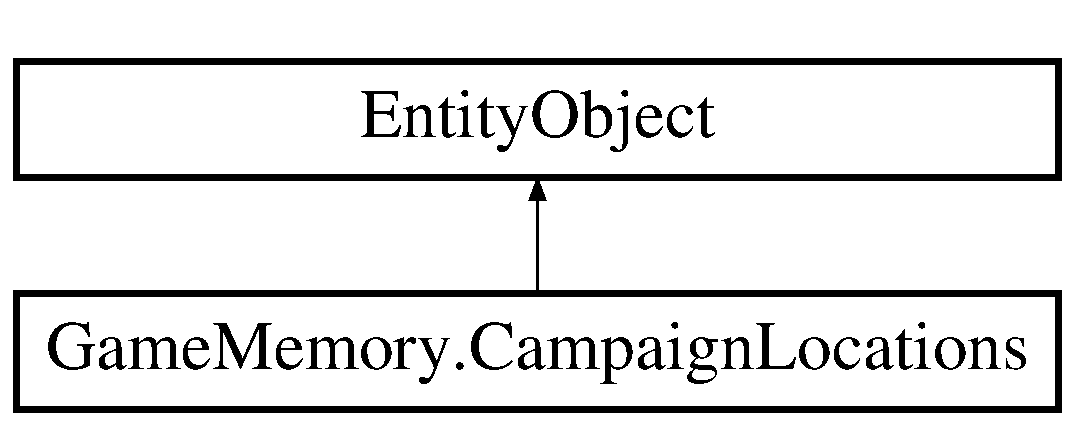
\includegraphics[height=2.000000cm]{class_game_memory_1_1_campaign_locations}
\end{center}
\end{figure}
\subsection*{Static Public Member Functions}
\begin{DoxyCompactItemize}
\item 
static \hyperlink{class_game_memory_1_1_campaign_locations}{Campaign\-Locations} \hyperlink{class_game_memory_1_1_campaign_locations_af7165452c80ac0217123e7aa3c30cd31}{Create\-Campaign\-Locations} (global\-::\-System.\-Int32 campaign\-Location\-Id)
\begin{DoxyCompactList}\small\item\em Crear un nuevo objeto \hyperlink{class_game_memory_1_1_campaign_locations}{Campaign\-Locations}. \end{DoxyCompactList}\end{DoxyCompactItemize}
\subsection*{Properties}
\begin{DoxyCompactItemize}
\item 
global\-::\-System.\-Int32 \hyperlink{class_game_memory_1_1_campaign_locations_a274c121c958554b8ab18ef8b4d2aaf92}{Campaign\-Location\-Id}\hspace{0.3cm}{\ttfamily  \mbox{[}get, set\mbox{]}}
\begin{DoxyCompactList}\small\item\em No hay documentación de metadatos disponible. \end{DoxyCompactList}\item 
global\-::\-System.\-String \hyperlink{class_game_memory_1_1_campaign_locations_a8cff8e401fb34c18237a7170f521f661}{Description}\hspace{0.3cm}{\ttfamily  \mbox{[}get, set\mbox{]}}
\begin{DoxyCompactList}\small\item\em No hay documentación de metadatos disponible. \end{DoxyCompactList}\item 
Entity\-Collection$<$ \hyperlink{class_game_memory_1_1_advert_campaigns}{Advert\-Campaigns} $>$ \hyperlink{class_game_memory_1_1_campaign_locations_a01592ca172f3fc4a7342aa232aefb2c5}{Advert\-Campaigns}\hspace{0.3cm}{\ttfamily  \mbox{[}get, set\mbox{]}}
\begin{DoxyCompactList}\small\item\em No hay documentación de metadatos disponible. \end{DoxyCompactList}\item 
Entity\-Collection$<$ \hyperlink{class_game_memory_1_1_advert_hosts}{Advert\-Hosts} $>$ \hyperlink{class_game_memory_1_1_campaign_locations_a5cd8ae0985a1191321033d26d09c5231}{Advert\-Hosts}\hspace{0.3cm}{\ttfamily  \mbox{[}get, set\mbox{]}}
\begin{DoxyCompactList}\small\item\em No hay documentación de metadatos disponible. \end{DoxyCompactList}\end{DoxyCompactItemize}


\subsection{Detailed Description}
No hay documentación de metadatos disponible. 



\subsection{Member Function Documentation}
\hypertarget{class_game_memory_1_1_campaign_locations_af7165452c80ac0217123e7aa3c30cd31}{\index{Game\-Memory\-::\-Campaign\-Locations@{Game\-Memory\-::\-Campaign\-Locations}!Create\-Campaign\-Locations@{Create\-Campaign\-Locations}}
\index{Create\-Campaign\-Locations@{Create\-Campaign\-Locations}!GameMemory::CampaignLocations@{Game\-Memory\-::\-Campaign\-Locations}}
\subsubsection[{Create\-Campaign\-Locations}]{\setlength{\rightskip}{0pt plus 5cm}static {\bf Campaign\-Locations} Game\-Memory.\-Campaign\-Locations.\-Create\-Campaign\-Locations (
\begin{DoxyParamCaption}
\item[{global\-::\-System.\-Int32}]{campaign\-Location\-Id}
\end{DoxyParamCaption}
)\hspace{0.3cm}{\ttfamily [static]}}}\label{class_game_memory_1_1_campaign_locations_af7165452c80ac0217123e7aa3c30cd31}


Crear un nuevo objeto \hyperlink{class_game_memory_1_1_campaign_locations}{Campaign\-Locations}. 


\begin{DoxyParams}{Parameters}
{\em campaign\-Location\-Id} & Valor inicial de la propiedad Campaign\-Location\-Id.\\
\hline
\end{DoxyParams}


\subsection{Property Documentation}
\hypertarget{class_game_memory_1_1_campaign_locations_a01592ca172f3fc4a7342aa232aefb2c5}{\index{Game\-Memory\-::\-Campaign\-Locations@{Game\-Memory\-::\-Campaign\-Locations}!Advert\-Campaigns@{Advert\-Campaigns}}
\index{Advert\-Campaigns@{Advert\-Campaigns}!GameMemory::CampaignLocations@{Game\-Memory\-::\-Campaign\-Locations}}
\subsubsection[{Advert\-Campaigns}]{\setlength{\rightskip}{0pt plus 5cm}Entity\-Collection$<${\bf Advert\-Campaigns}$>$ Game\-Memory.\-Campaign\-Locations.\-Advert\-Campaigns\hspace{0.3cm}{\ttfamily [get]}, {\ttfamily [set]}}}\label{class_game_memory_1_1_campaign_locations_a01592ca172f3fc4a7342aa232aefb2c5}


No hay documentación de metadatos disponible. 

\hypertarget{class_game_memory_1_1_campaign_locations_a5cd8ae0985a1191321033d26d09c5231}{\index{Game\-Memory\-::\-Campaign\-Locations@{Game\-Memory\-::\-Campaign\-Locations}!Advert\-Hosts@{Advert\-Hosts}}
\index{Advert\-Hosts@{Advert\-Hosts}!GameMemory::CampaignLocations@{Game\-Memory\-::\-Campaign\-Locations}}
\subsubsection[{Advert\-Hosts}]{\setlength{\rightskip}{0pt plus 5cm}Entity\-Collection$<${\bf Advert\-Hosts}$>$ Game\-Memory.\-Campaign\-Locations.\-Advert\-Hosts\hspace{0.3cm}{\ttfamily [get]}, {\ttfamily [set]}}}\label{class_game_memory_1_1_campaign_locations_a5cd8ae0985a1191321033d26d09c5231}


No hay documentación de metadatos disponible. 

\hypertarget{class_game_memory_1_1_campaign_locations_a274c121c958554b8ab18ef8b4d2aaf92}{\index{Game\-Memory\-::\-Campaign\-Locations@{Game\-Memory\-::\-Campaign\-Locations}!Campaign\-Location\-Id@{Campaign\-Location\-Id}}
\index{Campaign\-Location\-Id@{Campaign\-Location\-Id}!GameMemory::CampaignLocations@{Game\-Memory\-::\-Campaign\-Locations}}
\subsubsection[{Campaign\-Location\-Id}]{\setlength{\rightskip}{0pt plus 5cm}global.\-System.\-Int32 Game\-Memory.\-Campaign\-Locations.\-Campaign\-Location\-Id\hspace{0.3cm}{\ttfamily [get]}, {\ttfamily [set]}}}\label{class_game_memory_1_1_campaign_locations_a274c121c958554b8ab18ef8b4d2aaf92}


No hay documentación de metadatos disponible. 

\hypertarget{class_game_memory_1_1_campaign_locations_a8cff8e401fb34c18237a7170f521f661}{\index{Game\-Memory\-::\-Campaign\-Locations@{Game\-Memory\-::\-Campaign\-Locations}!Description@{Description}}
\index{Description@{Description}!GameMemory::CampaignLocations@{Game\-Memory\-::\-Campaign\-Locations}}
\subsubsection[{Description}]{\setlength{\rightskip}{0pt plus 5cm}global.\-System.\-String Game\-Memory.\-Campaign\-Locations.\-Description\hspace{0.3cm}{\ttfamily [get]}, {\ttfamily [set]}}}\label{class_game_memory_1_1_campaign_locations_a8cff8e401fb34c18237a7170f521f661}


No hay documentación de metadatos disponible. 



The documentation for this class was generated from the following file\-:\begin{DoxyCompactItemize}
\item 
D\-:/tesis\-Assembla/branches/\-Branch\-\_\-\-Tesis\-\_\-\-Sprint01/\-Dev/\-Interaction Module/\-Game\-Memory/\-Game\-Memory/O\-M\-K\-T.\-Designer.\-cs\end{DoxyCompactItemize}

\hypertarget{class_game_memory_1_1_campaign_states}{\section{Game\-Memory.\-Campaign\-States Class Reference}
\label{class_game_memory_1_1_campaign_states}\index{Game\-Memory.\-Campaign\-States@{Game\-Memory.\-Campaign\-States}}
}


No hay documentación de metadatos disponible.  


Inheritance diagram for Game\-Memory.\-Campaign\-States\-:\begin{figure}[H]
\begin{center}
\leavevmode
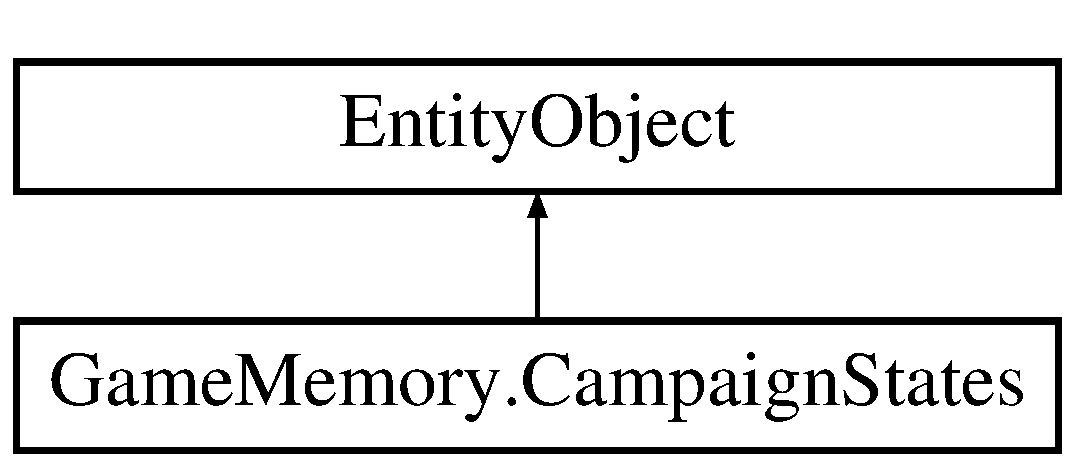
\includegraphics[height=2.000000cm]{class_game_memory_1_1_campaign_states}
\end{center}
\end{figure}
\subsection*{Static Public Member Functions}
\begin{DoxyCompactItemize}
\item 
static \hyperlink{class_game_memory_1_1_campaign_states}{Campaign\-States} \hyperlink{class_game_memory_1_1_campaign_states_add9051f7e065e73ad9ffaf36e2e103aa}{Create\-Campaign\-States} (global\-::\-System.\-Int32 campaign\-State\-Id)
\begin{DoxyCompactList}\small\item\em Crear un nuevo objeto \hyperlink{class_game_memory_1_1_campaign_states}{Campaign\-States}. \end{DoxyCompactList}\end{DoxyCompactItemize}
\subsection*{Properties}
\begin{DoxyCompactItemize}
\item 
global\-::\-System.\-Int32 \hyperlink{class_game_memory_1_1_campaign_states_a601afd4dcdde9340518a610a55469580}{Campaign\-State\-Id}\hspace{0.3cm}{\ttfamily  \mbox{[}get, set\mbox{]}}
\begin{DoxyCompactList}\small\item\em No hay documentación de metadatos disponible. \end{DoxyCompactList}\item 
global\-::\-System.\-String \hyperlink{class_game_memory_1_1_campaign_states_a4f99ca8ca1805ffe03998685fae7913c}{Description}\hspace{0.3cm}{\ttfamily  \mbox{[}get, set\mbox{]}}
\begin{DoxyCompactList}\small\item\em No hay documentación de metadatos disponible. \end{DoxyCompactList}\item 
Entity\-Collection$<$ \hyperlink{class_game_memory_1_1_advert_campaigns}{Advert\-Campaigns} $>$ \hyperlink{class_game_memory_1_1_campaign_states_a4e6c871f2c55f0e02c9b6242baf6ef5c}{Advert\-Campaigns}\hspace{0.3cm}{\ttfamily  \mbox{[}get, set\mbox{]}}
\begin{DoxyCompactList}\small\item\em No hay documentación de metadatos disponible. \end{DoxyCompactList}\end{DoxyCompactItemize}


\subsection{Detailed Description}
No hay documentación de metadatos disponible. 



\subsection{Member Function Documentation}
\hypertarget{class_game_memory_1_1_campaign_states_add9051f7e065e73ad9ffaf36e2e103aa}{\index{Game\-Memory\-::\-Campaign\-States@{Game\-Memory\-::\-Campaign\-States}!Create\-Campaign\-States@{Create\-Campaign\-States}}
\index{Create\-Campaign\-States@{Create\-Campaign\-States}!GameMemory::CampaignStates@{Game\-Memory\-::\-Campaign\-States}}
\subsubsection[{Create\-Campaign\-States}]{\setlength{\rightskip}{0pt plus 5cm}static {\bf Campaign\-States} Game\-Memory.\-Campaign\-States.\-Create\-Campaign\-States (
\begin{DoxyParamCaption}
\item[{global\-::\-System.\-Int32}]{campaign\-State\-Id}
\end{DoxyParamCaption}
)\hspace{0.3cm}{\ttfamily [static]}}}\label{class_game_memory_1_1_campaign_states_add9051f7e065e73ad9ffaf36e2e103aa}


Crear un nuevo objeto \hyperlink{class_game_memory_1_1_campaign_states}{Campaign\-States}. 


\begin{DoxyParams}{Parameters}
{\em campaign\-State\-Id} & Valor inicial de la propiedad Campaign\-State\-Id.\\
\hline
\end{DoxyParams}


\subsection{Property Documentation}
\hypertarget{class_game_memory_1_1_campaign_states_a4e6c871f2c55f0e02c9b6242baf6ef5c}{\index{Game\-Memory\-::\-Campaign\-States@{Game\-Memory\-::\-Campaign\-States}!Advert\-Campaigns@{Advert\-Campaigns}}
\index{Advert\-Campaigns@{Advert\-Campaigns}!GameMemory::CampaignStates@{Game\-Memory\-::\-Campaign\-States}}
\subsubsection[{Advert\-Campaigns}]{\setlength{\rightskip}{0pt plus 5cm}Entity\-Collection$<${\bf Advert\-Campaigns}$>$ Game\-Memory.\-Campaign\-States.\-Advert\-Campaigns\hspace{0.3cm}{\ttfamily [get]}, {\ttfamily [set]}}}\label{class_game_memory_1_1_campaign_states_a4e6c871f2c55f0e02c9b6242baf6ef5c}


No hay documentación de metadatos disponible. 

\hypertarget{class_game_memory_1_1_campaign_states_a601afd4dcdde9340518a610a55469580}{\index{Game\-Memory\-::\-Campaign\-States@{Game\-Memory\-::\-Campaign\-States}!Campaign\-State\-Id@{Campaign\-State\-Id}}
\index{Campaign\-State\-Id@{Campaign\-State\-Id}!GameMemory::CampaignStates@{Game\-Memory\-::\-Campaign\-States}}
\subsubsection[{Campaign\-State\-Id}]{\setlength{\rightskip}{0pt plus 5cm}global.\-System.\-Int32 Game\-Memory.\-Campaign\-States.\-Campaign\-State\-Id\hspace{0.3cm}{\ttfamily [get]}, {\ttfamily [set]}}}\label{class_game_memory_1_1_campaign_states_a601afd4dcdde9340518a610a55469580}


No hay documentación de metadatos disponible. 

\hypertarget{class_game_memory_1_1_campaign_states_a4f99ca8ca1805ffe03998685fae7913c}{\index{Game\-Memory\-::\-Campaign\-States@{Game\-Memory\-::\-Campaign\-States}!Description@{Description}}
\index{Description@{Description}!GameMemory::CampaignStates@{Game\-Memory\-::\-Campaign\-States}}
\subsubsection[{Description}]{\setlength{\rightskip}{0pt plus 5cm}global.\-System.\-String Game\-Memory.\-Campaign\-States.\-Description\hspace{0.3cm}{\ttfamily [get]}, {\ttfamily [set]}}}\label{class_game_memory_1_1_campaign_states_a4f99ca8ca1805ffe03998685fae7913c}


No hay documentación de metadatos disponible. 



The documentation for this class was generated from the following file\-:\begin{DoxyCompactItemize}
\item 
D\-:/tesis\-Assembla/branches/\-Branch\-\_\-\-Tesis\-\_\-\-Sprint01/\-Dev/\-Interaction Module/\-Game\-Memory/\-Game\-Memory/O\-M\-K\-T.\-Designer.\-cs\end{DoxyCompactItemize}

\hypertarget{class_game_memory_1_1_campaign_types}{\section{Game\-Memory.\-Campaign\-Types Class Reference}
\label{class_game_memory_1_1_campaign_types}\index{Game\-Memory.\-Campaign\-Types@{Game\-Memory.\-Campaign\-Types}}
}


No hay documentación de metadatos disponible.  


Inheritance diagram for Game\-Memory.\-Campaign\-Types\-:\begin{figure}[H]
\begin{center}
\leavevmode
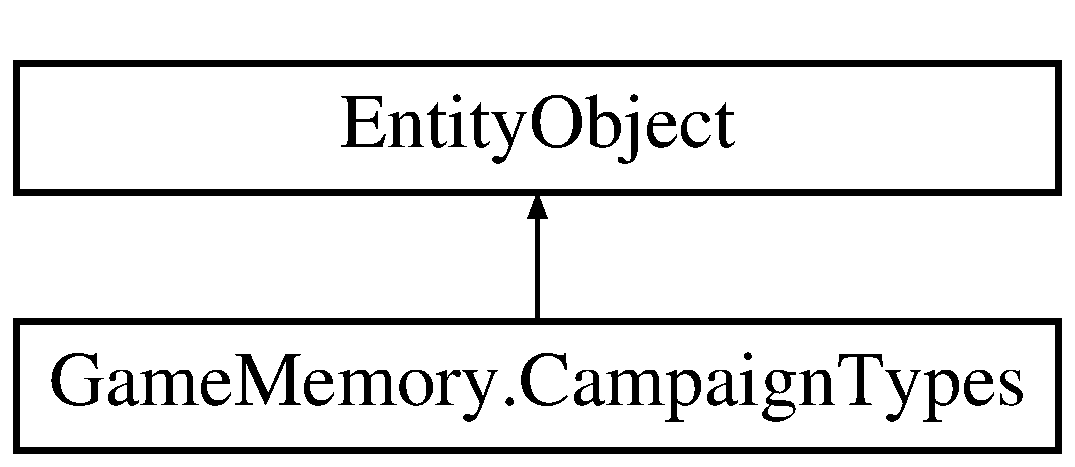
\includegraphics[height=2.000000cm]{class_game_memory_1_1_campaign_types}
\end{center}
\end{figure}
\subsection*{Static Public Member Functions}
\begin{DoxyCompactItemize}
\item 
static \hyperlink{class_game_memory_1_1_campaign_types}{Campaign\-Types} \hyperlink{class_game_memory_1_1_campaign_types_a0a6697f45e1d4d17ee4b1b49338662d1}{Create\-Campaign\-Types} (global\-::\-System.\-Int32 campaign\-Type\-Id)
\begin{DoxyCompactList}\small\item\em Crear un nuevo objeto \hyperlink{class_game_memory_1_1_campaign_types}{Campaign\-Types}. \end{DoxyCompactList}\end{DoxyCompactItemize}
\subsection*{Properties}
\begin{DoxyCompactItemize}
\item 
global\-::\-System.\-Int32 \hyperlink{class_game_memory_1_1_campaign_types_ab534e8f9389bed7b5d6ecb86a17518b8}{Campaign\-Type\-Id}\hspace{0.3cm}{\ttfamily  \mbox{[}get, set\mbox{]}}
\begin{DoxyCompactList}\small\item\em No hay documentación de metadatos disponible. \end{DoxyCompactList}\item 
global\-::\-System.\-String \hyperlink{class_game_memory_1_1_campaign_types_a24dabf7fdd3c80cd369958be0e7b846d}{Name}\hspace{0.3cm}{\ttfamily  \mbox{[}get, set\mbox{]}}
\begin{DoxyCompactList}\small\item\em No hay documentación de metadatos disponible. \end{DoxyCompactList}\item 
global\-::\-System.\-String \hyperlink{class_game_memory_1_1_campaign_types_a10d33d848dc2aaefd8e83d501579e172}{Description}\hspace{0.3cm}{\ttfamily  \mbox{[}get, set\mbox{]}}
\begin{DoxyCompactList}\small\item\em No hay documentación de metadatos disponible. \end{DoxyCompactList}\item 
Entity\-Collection$<$ \hyperlink{class_game_memory_1_1_advert_campaigns}{Advert\-Campaigns} $>$ \hyperlink{class_game_memory_1_1_campaign_types_a7ce779c5a0e20b2b0a1270306afda16d}{Advert\-Campaigns}\hspace{0.3cm}{\ttfamily  \mbox{[}get, set\mbox{]}}
\begin{DoxyCompactList}\small\item\em No hay documentación de metadatos disponible. \end{DoxyCompactList}\end{DoxyCompactItemize}


\subsection{Detailed Description}
No hay documentación de metadatos disponible. 



\subsection{Member Function Documentation}
\hypertarget{class_game_memory_1_1_campaign_types_a0a6697f45e1d4d17ee4b1b49338662d1}{\index{Game\-Memory\-::\-Campaign\-Types@{Game\-Memory\-::\-Campaign\-Types}!Create\-Campaign\-Types@{Create\-Campaign\-Types}}
\index{Create\-Campaign\-Types@{Create\-Campaign\-Types}!GameMemory::CampaignTypes@{Game\-Memory\-::\-Campaign\-Types}}
\subsubsection[{Create\-Campaign\-Types}]{\setlength{\rightskip}{0pt plus 5cm}static {\bf Campaign\-Types} Game\-Memory.\-Campaign\-Types.\-Create\-Campaign\-Types (
\begin{DoxyParamCaption}
\item[{global\-::\-System.\-Int32}]{campaign\-Type\-Id}
\end{DoxyParamCaption}
)\hspace{0.3cm}{\ttfamily [static]}}}\label{class_game_memory_1_1_campaign_types_a0a6697f45e1d4d17ee4b1b49338662d1}


Crear un nuevo objeto \hyperlink{class_game_memory_1_1_campaign_types}{Campaign\-Types}. 


\begin{DoxyParams}{Parameters}
{\em campaign\-Type\-Id} & Valor inicial de la propiedad Campaign\-Type\-Id.\\
\hline
\end{DoxyParams}


\subsection{Property Documentation}
\hypertarget{class_game_memory_1_1_campaign_types_a7ce779c5a0e20b2b0a1270306afda16d}{\index{Game\-Memory\-::\-Campaign\-Types@{Game\-Memory\-::\-Campaign\-Types}!Advert\-Campaigns@{Advert\-Campaigns}}
\index{Advert\-Campaigns@{Advert\-Campaigns}!GameMemory::CampaignTypes@{Game\-Memory\-::\-Campaign\-Types}}
\subsubsection[{Advert\-Campaigns}]{\setlength{\rightskip}{0pt plus 5cm}Entity\-Collection$<${\bf Advert\-Campaigns}$>$ Game\-Memory.\-Campaign\-Types.\-Advert\-Campaigns\hspace{0.3cm}{\ttfamily [get]}, {\ttfamily [set]}}}\label{class_game_memory_1_1_campaign_types_a7ce779c5a0e20b2b0a1270306afda16d}


No hay documentación de metadatos disponible. 

\hypertarget{class_game_memory_1_1_campaign_types_ab534e8f9389bed7b5d6ecb86a17518b8}{\index{Game\-Memory\-::\-Campaign\-Types@{Game\-Memory\-::\-Campaign\-Types}!Campaign\-Type\-Id@{Campaign\-Type\-Id}}
\index{Campaign\-Type\-Id@{Campaign\-Type\-Id}!GameMemory::CampaignTypes@{Game\-Memory\-::\-Campaign\-Types}}
\subsubsection[{Campaign\-Type\-Id}]{\setlength{\rightskip}{0pt plus 5cm}global.\-System.\-Int32 Game\-Memory.\-Campaign\-Types.\-Campaign\-Type\-Id\hspace{0.3cm}{\ttfamily [get]}, {\ttfamily [set]}}}\label{class_game_memory_1_1_campaign_types_ab534e8f9389bed7b5d6ecb86a17518b8}


No hay documentación de metadatos disponible. 

\hypertarget{class_game_memory_1_1_campaign_types_a10d33d848dc2aaefd8e83d501579e172}{\index{Game\-Memory\-::\-Campaign\-Types@{Game\-Memory\-::\-Campaign\-Types}!Description@{Description}}
\index{Description@{Description}!GameMemory::CampaignTypes@{Game\-Memory\-::\-Campaign\-Types}}
\subsubsection[{Description}]{\setlength{\rightskip}{0pt plus 5cm}global.\-System.\-String Game\-Memory.\-Campaign\-Types.\-Description\hspace{0.3cm}{\ttfamily [get]}, {\ttfamily [set]}}}\label{class_game_memory_1_1_campaign_types_a10d33d848dc2aaefd8e83d501579e172}


No hay documentación de metadatos disponible. 

\hypertarget{class_game_memory_1_1_campaign_types_a24dabf7fdd3c80cd369958be0e7b846d}{\index{Game\-Memory\-::\-Campaign\-Types@{Game\-Memory\-::\-Campaign\-Types}!Name@{Name}}
\index{Name@{Name}!GameMemory::CampaignTypes@{Game\-Memory\-::\-Campaign\-Types}}
\subsubsection[{Name}]{\setlength{\rightskip}{0pt plus 5cm}global.\-System.\-String Game\-Memory.\-Campaign\-Types.\-Name\hspace{0.3cm}{\ttfamily [get]}, {\ttfamily [set]}}}\label{class_game_memory_1_1_campaign_types_a24dabf7fdd3c80cd369958be0e7b846d}


No hay documentación de metadatos disponible. 



The documentation for this class was generated from the following file\-:\begin{DoxyCompactItemize}
\item 
D\-:/tesis\-Assembla/branches/\-Branch\-\_\-\-Tesis\-\_\-\-Sprint01/\-Dev/\-Interaction Module/\-Game\-Memory/\-Game\-Memory/O\-M\-K\-T.\-Designer.\-cs\end{DoxyCompactItemize}

\hypertarget{class_game_memory_1_1_catalog_detail_interactions}{\section{Game\-Memory.\-Catalog\-Detail\-Interactions Class Reference}
\label{class_game_memory_1_1_catalog_detail_interactions}\index{Game\-Memory.\-Catalog\-Detail\-Interactions@{Game\-Memory.\-Catalog\-Detail\-Interactions}}
}


No hay documentación de metadatos disponible.  


Inheritance diagram for Game\-Memory.\-Catalog\-Detail\-Interactions\-:\begin{figure}[H]
\begin{center}
\leavevmode
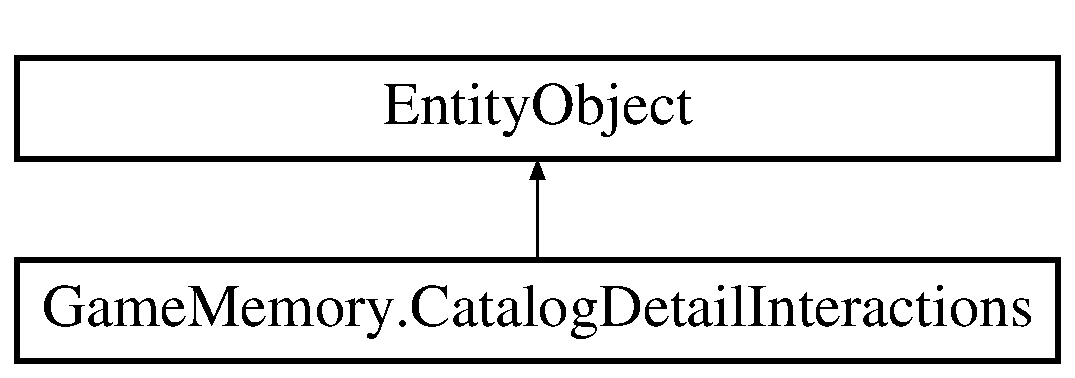
\includegraphics[height=2.000000cm]{class_game_memory_1_1_catalog_detail_interactions}
\end{center}
\end{figure}
\subsection*{Static Public Member Functions}
\begin{DoxyCompactItemize}
\item 
static \hyperlink{class_game_memory_1_1_catalog_detail_interactions}{Catalog\-Detail\-Interactions} \hyperlink{class_game_memory_1_1_catalog_detail_interactions_a334021a70e2896564978fc2ded9e451c}{Create\-Catalog\-Detail\-Interactions} (global\-::\-System.\-Int32 catalog\-Detail\-Interaction\-I\-D, global\-::\-System.\-Int32 catalog\-Detail\-I\-D, global\-::\-System.\-Boolean view, global\-::\-System.\-Date\-Time start\-Datetime)
\begin{DoxyCompactList}\small\item\em Crear un nuevo objeto \hyperlink{class_game_memory_1_1_catalog_detail_interactions}{Catalog\-Detail\-Interactions}. \end{DoxyCompactList}\end{DoxyCompactItemize}
\subsection*{Properties}
\begin{DoxyCompactItemize}
\item 
global\-::\-System.\-Int32 \hyperlink{class_game_memory_1_1_catalog_detail_interactions_a069a81f58e0a578f38eb9ecb69bb5a7b}{Catalog\-Detail\-Interaction\-I\-D}\hspace{0.3cm}{\ttfamily  \mbox{[}get, set\mbox{]}}
\begin{DoxyCompactList}\small\item\em No hay documentación de metadatos disponible. \end{DoxyCompactList}\item 
global\-::\-System.\-Int32 \hyperlink{class_game_memory_1_1_catalog_detail_interactions_a595e63da355b8a69ec4da9038aaaee29}{Catalog\-Detail\-I\-D}\hspace{0.3cm}{\ttfamily  \mbox{[}get, set\mbox{]}}
\begin{DoxyCompactList}\small\item\em No hay documentación de metadatos disponible. \end{DoxyCompactList}\item 
global\-::\-System.\-Boolean \hyperlink{class_game_memory_1_1_catalog_detail_interactions_aa1066cee4581a0ec9f0169f6336d75b8}{View}\hspace{0.3cm}{\ttfamily  \mbox{[}get, set\mbox{]}}
\begin{DoxyCompactList}\small\item\em No hay documentación de metadatos disponible. \end{DoxyCompactList}\item 
Nullable$<$ global\-::\-System.\-Boolean $>$ \hyperlink{class_game_memory_1_1_catalog_detail_interactions_a4f0e09f1191b173af90719683f166595}{Like}\hspace{0.3cm}{\ttfamily  \mbox{[}get, set\mbox{]}}
\begin{DoxyCompactList}\small\item\em No hay documentación de metadatos disponible. \end{DoxyCompactList}\item 
global\-::\-System.\-Date\-Time \hyperlink{class_game_memory_1_1_catalog_detail_interactions_a39bb069512ca0a6abdf9df3d0aa54cf0}{Start\-Datetime}\hspace{0.3cm}{\ttfamily  \mbox{[}get, set\mbox{]}}
\begin{DoxyCompactList}\small\item\em No hay documentación de metadatos disponible. \end{DoxyCompactList}\item 
Nullable$<$ global\-::\-System.\-Date\-Time $>$ \hyperlink{class_game_memory_1_1_catalog_detail_interactions_a14d6e49b9317999c0c9fb466c863b98a}{End\-Datetime}\hspace{0.3cm}{\ttfamily  \mbox{[}get, set\mbox{]}}
\begin{DoxyCompactList}\small\item\em No hay documentación de metadatos disponible. \end{DoxyCompactList}\item 
Nullable$<$ global\-::\-System.\-Int32 $>$ \hyperlink{class_game_memory_1_1_catalog_detail_interactions_abf1ec4f566957f8c8d8d70a6f3f775e6}{Time\-Elapsed}\hspace{0.3cm}{\ttfamily  \mbox{[}get, set\mbox{]}}
\begin{DoxyCompactList}\small\item\em No hay documentación de metadatos disponible. \end{DoxyCompactList}\item 
\hyperlink{class_game_memory_1_1_catalog_details}{Catalog\-Details} \hyperlink{class_game_memory_1_1_catalog_detail_interactions_a232363d89fa16413a33ec13cbf7a8128}{Catalog\-Details}\hspace{0.3cm}{\ttfamily  \mbox{[}get, set\mbox{]}}
\begin{DoxyCompactList}\small\item\em No hay documentación de metadatos disponible. \end{DoxyCompactList}\item 
Entity\-Reference$<$ \hyperlink{class_game_memory_1_1_catalog_details}{Catalog\-Details} $>$ \hyperlink{class_game_memory_1_1_catalog_detail_interactions_a3b322f224a3556ae0a67754c37dec51d}{Catalog\-Details\-Reference}\hspace{0.3cm}{\ttfamily  \mbox{[}get, set\mbox{]}}
\begin{DoxyCompactList}\small\item\em No hay documentación de metadatos disponible. \end{DoxyCompactList}\end{DoxyCompactItemize}


\subsection{Detailed Description}
No hay documentación de metadatos disponible. 



\subsection{Member Function Documentation}
\hypertarget{class_game_memory_1_1_catalog_detail_interactions_a334021a70e2896564978fc2ded9e451c}{\index{Game\-Memory\-::\-Catalog\-Detail\-Interactions@{Game\-Memory\-::\-Catalog\-Detail\-Interactions}!Create\-Catalog\-Detail\-Interactions@{Create\-Catalog\-Detail\-Interactions}}
\index{Create\-Catalog\-Detail\-Interactions@{Create\-Catalog\-Detail\-Interactions}!GameMemory::CatalogDetailInteractions@{Game\-Memory\-::\-Catalog\-Detail\-Interactions}}
\subsubsection[{Create\-Catalog\-Detail\-Interactions}]{\setlength{\rightskip}{0pt plus 5cm}static {\bf Catalog\-Detail\-Interactions} Game\-Memory.\-Catalog\-Detail\-Interactions.\-Create\-Catalog\-Detail\-Interactions (
\begin{DoxyParamCaption}
\item[{global\-::\-System.\-Int32}]{catalog\-Detail\-Interaction\-I\-D, }
\item[{global\-::\-System.\-Int32}]{catalog\-Detail\-I\-D, }
\item[{global\-::\-System.\-Boolean}]{view, }
\item[{global\-::\-System.\-Date\-Time}]{start\-Datetime}
\end{DoxyParamCaption}
)\hspace{0.3cm}{\ttfamily [static]}}}\label{class_game_memory_1_1_catalog_detail_interactions_a334021a70e2896564978fc2ded9e451c}


Crear un nuevo objeto \hyperlink{class_game_memory_1_1_catalog_detail_interactions}{Catalog\-Detail\-Interactions}. 


\begin{DoxyParams}{Parameters}
{\em catalog\-Detail\-Interaction\-I\-D} & Valor inicial de la propiedad Catalog\-Detail\-Interaction\-I\-D.\\
\hline
{\em catalog\-Detail\-I\-D} & Valor inicial de la propiedad Catalog\-Detail\-I\-D.\\
\hline
{\em view} & Valor inicial de la propiedad View.\\
\hline
{\em start\-Datetime} & Valor inicial de la propiedad Start\-Datetime.\\
\hline
\end{DoxyParams}


\subsection{Property Documentation}
\hypertarget{class_game_memory_1_1_catalog_detail_interactions_a595e63da355b8a69ec4da9038aaaee29}{\index{Game\-Memory\-::\-Catalog\-Detail\-Interactions@{Game\-Memory\-::\-Catalog\-Detail\-Interactions}!Catalog\-Detail\-I\-D@{Catalog\-Detail\-I\-D}}
\index{Catalog\-Detail\-I\-D@{Catalog\-Detail\-I\-D}!GameMemory::CatalogDetailInteractions@{Game\-Memory\-::\-Catalog\-Detail\-Interactions}}
\subsubsection[{Catalog\-Detail\-I\-D}]{\setlength{\rightskip}{0pt plus 5cm}global.\-System.\-Int32 Game\-Memory.\-Catalog\-Detail\-Interactions.\-Catalog\-Detail\-I\-D\hspace{0.3cm}{\ttfamily [get]}, {\ttfamily [set]}}}\label{class_game_memory_1_1_catalog_detail_interactions_a595e63da355b8a69ec4da9038aaaee29}


No hay documentación de metadatos disponible. 

\hypertarget{class_game_memory_1_1_catalog_detail_interactions_a069a81f58e0a578f38eb9ecb69bb5a7b}{\index{Game\-Memory\-::\-Catalog\-Detail\-Interactions@{Game\-Memory\-::\-Catalog\-Detail\-Interactions}!Catalog\-Detail\-Interaction\-I\-D@{Catalog\-Detail\-Interaction\-I\-D}}
\index{Catalog\-Detail\-Interaction\-I\-D@{Catalog\-Detail\-Interaction\-I\-D}!GameMemory::CatalogDetailInteractions@{Game\-Memory\-::\-Catalog\-Detail\-Interactions}}
\subsubsection[{Catalog\-Detail\-Interaction\-I\-D}]{\setlength{\rightskip}{0pt plus 5cm}global.\-System.\-Int32 Game\-Memory.\-Catalog\-Detail\-Interactions.\-Catalog\-Detail\-Interaction\-I\-D\hspace{0.3cm}{\ttfamily [get]}, {\ttfamily [set]}}}\label{class_game_memory_1_1_catalog_detail_interactions_a069a81f58e0a578f38eb9ecb69bb5a7b}


No hay documentación de metadatos disponible. 

\hypertarget{class_game_memory_1_1_catalog_detail_interactions_a232363d89fa16413a33ec13cbf7a8128}{\index{Game\-Memory\-::\-Catalog\-Detail\-Interactions@{Game\-Memory\-::\-Catalog\-Detail\-Interactions}!Catalog\-Details@{Catalog\-Details}}
\index{Catalog\-Details@{Catalog\-Details}!GameMemory::CatalogDetailInteractions@{Game\-Memory\-::\-Catalog\-Detail\-Interactions}}
\subsubsection[{Catalog\-Details}]{\setlength{\rightskip}{0pt plus 5cm}{\bf Catalog\-Details} Game\-Memory.\-Catalog\-Detail\-Interactions.\-Catalog\-Details\hspace{0.3cm}{\ttfamily [get]}, {\ttfamily [set]}}}\label{class_game_memory_1_1_catalog_detail_interactions_a232363d89fa16413a33ec13cbf7a8128}


No hay documentación de metadatos disponible. 

\hypertarget{class_game_memory_1_1_catalog_detail_interactions_a3b322f224a3556ae0a67754c37dec51d}{\index{Game\-Memory\-::\-Catalog\-Detail\-Interactions@{Game\-Memory\-::\-Catalog\-Detail\-Interactions}!Catalog\-Details\-Reference@{Catalog\-Details\-Reference}}
\index{Catalog\-Details\-Reference@{Catalog\-Details\-Reference}!GameMemory::CatalogDetailInteractions@{Game\-Memory\-::\-Catalog\-Detail\-Interactions}}
\subsubsection[{Catalog\-Details\-Reference}]{\setlength{\rightskip}{0pt plus 5cm}Entity\-Reference$<${\bf Catalog\-Details}$>$ Game\-Memory.\-Catalog\-Detail\-Interactions.\-Catalog\-Details\-Reference\hspace{0.3cm}{\ttfamily [get]}, {\ttfamily [set]}}}\label{class_game_memory_1_1_catalog_detail_interactions_a3b322f224a3556ae0a67754c37dec51d}


No hay documentación de metadatos disponible. 

\hypertarget{class_game_memory_1_1_catalog_detail_interactions_a14d6e49b9317999c0c9fb466c863b98a}{\index{Game\-Memory\-::\-Catalog\-Detail\-Interactions@{Game\-Memory\-::\-Catalog\-Detail\-Interactions}!End\-Datetime@{End\-Datetime}}
\index{End\-Datetime@{End\-Datetime}!GameMemory::CatalogDetailInteractions@{Game\-Memory\-::\-Catalog\-Detail\-Interactions}}
\subsubsection[{End\-Datetime}]{\setlength{\rightskip}{0pt plus 5cm}Nullable$<$global.\-System.\-Date\-Time$>$ Game\-Memory.\-Catalog\-Detail\-Interactions.\-End\-Datetime\hspace{0.3cm}{\ttfamily [get]}, {\ttfamily [set]}}}\label{class_game_memory_1_1_catalog_detail_interactions_a14d6e49b9317999c0c9fb466c863b98a}


No hay documentación de metadatos disponible. 

\hypertarget{class_game_memory_1_1_catalog_detail_interactions_a4f0e09f1191b173af90719683f166595}{\index{Game\-Memory\-::\-Catalog\-Detail\-Interactions@{Game\-Memory\-::\-Catalog\-Detail\-Interactions}!Like@{Like}}
\index{Like@{Like}!GameMemory::CatalogDetailInteractions@{Game\-Memory\-::\-Catalog\-Detail\-Interactions}}
\subsubsection[{Like}]{\setlength{\rightskip}{0pt plus 5cm}Nullable$<$global.\-System.\-Boolean$>$ Game\-Memory.\-Catalog\-Detail\-Interactions.\-Like\hspace{0.3cm}{\ttfamily [get]}, {\ttfamily [set]}}}\label{class_game_memory_1_1_catalog_detail_interactions_a4f0e09f1191b173af90719683f166595}


No hay documentación de metadatos disponible. 

\hypertarget{class_game_memory_1_1_catalog_detail_interactions_a39bb069512ca0a6abdf9df3d0aa54cf0}{\index{Game\-Memory\-::\-Catalog\-Detail\-Interactions@{Game\-Memory\-::\-Catalog\-Detail\-Interactions}!Start\-Datetime@{Start\-Datetime}}
\index{Start\-Datetime@{Start\-Datetime}!GameMemory::CatalogDetailInteractions@{Game\-Memory\-::\-Catalog\-Detail\-Interactions}}
\subsubsection[{Start\-Datetime}]{\setlength{\rightskip}{0pt plus 5cm}global.\-System.\-Date\-Time Game\-Memory.\-Catalog\-Detail\-Interactions.\-Start\-Datetime\hspace{0.3cm}{\ttfamily [get]}, {\ttfamily [set]}}}\label{class_game_memory_1_1_catalog_detail_interactions_a39bb069512ca0a6abdf9df3d0aa54cf0}


No hay documentación de metadatos disponible. 

\hypertarget{class_game_memory_1_1_catalog_detail_interactions_abf1ec4f566957f8c8d8d70a6f3f775e6}{\index{Game\-Memory\-::\-Catalog\-Detail\-Interactions@{Game\-Memory\-::\-Catalog\-Detail\-Interactions}!Time\-Elapsed@{Time\-Elapsed}}
\index{Time\-Elapsed@{Time\-Elapsed}!GameMemory::CatalogDetailInteractions@{Game\-Memory\-::\-Catalog\-Detail\-Interactions}}
\subsubsection[{Time\-Elapsed}]{\setlength{\rightskip}{0pt plus 5cm}Nullable$<$global.\-System.\-Int32$>$ Game\-Memory.\-Catalog\-Detail\-Interactions.\-Time\-Elapsed\hspace{0.3cm}{\ttfamily [get]}, {\ttfamily [set]}}}\label{class_game_memory_1_1_catalog_detail_interactions_abf1ec4f566957f8c8d8d70a6f3f775e6}


No hay documentación de metadatos disponible. 

\hypertarget{class_game_memory_1_1_catalog_detail_interactions_aa1066cee4581a0ec9f0169f6336d75b8}{\index{Game\-Memory\-::\-Catalog\-Detail\-Interactions@{Game\-Memory\-::\-Catalog\-Detail\-Interactions}!View@{View}}
\index{View@{View}!GameMemory::CatalogDetailInteractions@{Game\-Memory\-::\-Catalog\-Detail\-Interactions}}
\subsubsection[{View}]{\setlength{\rightskip}{0pt plus 5cm}global.\-System.\-Boolean Game\-Memory.\-Catalog\-Detail\-Interactions.\-View\hspace{0.3cm}{\ttfamily [get]}, {\ttfamily [set]}}}\label{class_game_memory_1_1_catalog_detail_interactions_aa1066cee4581a0ec9f0169f6336d75b8}


No hay documentación de metadatos disponible. 



The documentation for this class was generated from the following file\-:\begin{DoxyCompactItemize}
\item 
D\-:/tesis\-Assembla/branches/\-Branch\-\_\-\-Tesis\-\_\-\-Sprint01/\-Dev/\-Interaction Module/\-Game\-Memory/\-Game\-Memory/O\-M\-K\-T.\-Designer.\-cs\end{DoxyCompactItemize}

\hypertarget{class_game_memory_1_1_catalog_details}{\section{Game\-Memory.\-Catalog\-Details Class Reference}
\label{class_game_memory_1_1_catalog_details}\index{Game\-Memory.\-Catalog\-Details@{Game\-Memory.\-Catalog\-Details}}
}


No hay documentación de metadatos disponible.  


Inheritance diagram for Game\-Memory.\-Catalog\-Details\-:\begin{figure}[H]
\begin{center}
\leavevmode
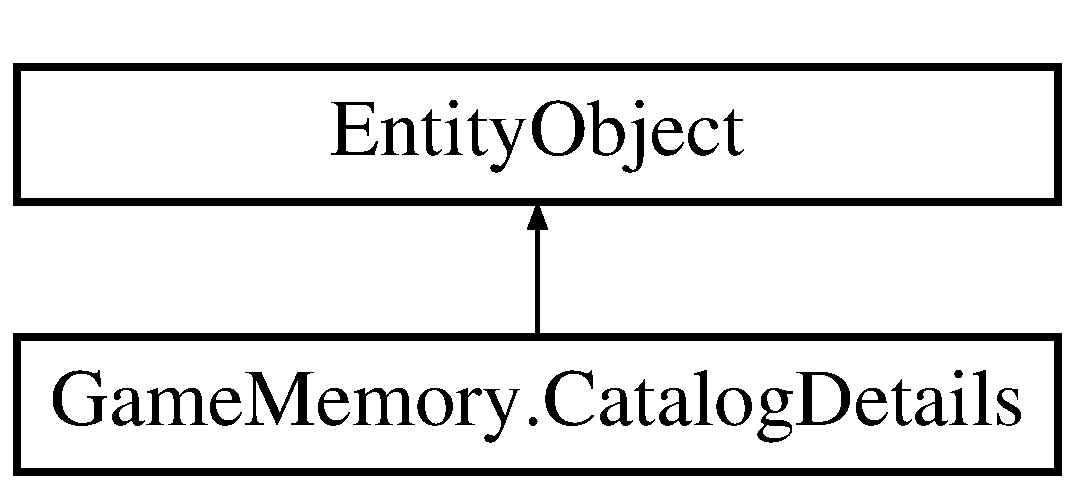
\includegraphics[height=2.000000cm]{class_game_memory_1_1_catalog_details}
\end{center}
\end{figure}
\subsection*{Static Public Member Functions}
\begin{DoxyCompactItemize}
\item 
static \hyperlink{class_game_memory_1_1_catalog_details}{Catalog\-Details} \hyperlink{class_game_memory_1_1_catalog_details_a4981cf637877d8c711145ae9d88e68af}{Create\-Catalog\-Details} (global\-::\-System.\-Int32 catalog\-Detail\-Id, global\-::\-System.\-Int32 advert\-Id, global\-::\-System.\-Int32 position, global\-::\-System.\-Int32 commercial\-Product\-Id, global\-::\-System.\-Double discount)
\begin{DoxyCompactList}\small\item\em Crear un nuevo objeto \hyperlink{class_game_memory_1_1_catalog_details}{Catalog\-Details}. \end{DoxyCompactList}\end{DoxyCompactItemize}
\subsection*{Properties}
\begin{DoxyCompactItemize}
\item 
global\-::\-System.\-Int32 \hyperlink{class_game_memory_1_1_catalog_details_a29a305600ee6d70b918347bcd40a3c81}{Catalog\-Detail\-Id}\hspace{0.3cm}{\ttfamily  \mbox{[}get, set\mbox{]}}
\begin{DoxyCompactList}\small\item\em No hay documentación de metadatos disponible. \end{DoxyCompactList}\item 
global\-::\-System.\-Int32 \hyperlink{class_game_memory_1_1_catalog_details_a32f193effd2e8f0b2704a630aac83568}{Advert\-Id}\hspace{0.3cm}{\ttfamily  \mbox{[}get, set\mbox{]}}
\begin{DoxyCompactList}\small\item\em No hay documentación de metadatos disponible. \end{DoxyCompactList}\item 
global\-::\-System.\-Int32 \hyperlink{class_game_memory_1_1_catalog_details_a4b69bad6ac79c610a167f11271a2acf4}{Position}\hspace{0.3cm}{\ttfamily  \mbox{[}get, set\mbox{]}}
\begin{DoxyCompactList}\small\item\em No hay documentación de metadatos disponible. \end{DoxyCompactList}\item 
global\-::\-System.\-Int32 \hyperlink{class_game_memory_1_1_catalog_details_a18e97c03d1ac3af15e49bb0059ae3a2a}{Commercial\-Product\-Id}\hspace{0.3cm}{\ttfamily  \mbox{[}get, set\mbox{]}}
\begin{DoxyCompactList}\small\item\em No hay documentación de metadatos disponible. \end{DoxyCompactList}\item 
global\-::\-System.\-Double \hyperlink{class_game_memory_1_1_catalog_details_aed76f865302ee9147bffc9fec748bb5f}{Discount}\hspace{0.3cm}{\ttfamily  \mbox{[}get, set\mbox{]}}
\begin{DoxyCompactList}\small\item\em No hay documentación de metadatos disponible. \end{DoxyCompactList}\item 
global\-::\-System.\-String \hyperlink{class_game_memory_1_1_catalog_details_a0602f3d016450f9cb6f0d3ff955bac2b}{Q\-R\-Code}\hspace{0.3cm}{\ttfamily  \mbox{[}get, set\mbox{]}}
\begin{DoxyCompactList}\small\item\em No hay documentación de metadatos disponible. \end{DoxyCompactList}\item 
global\-::\-System.\-String \hyperlink{class_game_memory_1_1_catalog_details_ad9b810e2b2a259a71e5ffa8b83bbe47c}{Link}\hspace{0.3cm}{\ttfamily  \mbox{[}get, set\mbox{]}}
\begin{DoxyCompactList}\small\item\em No hay documentación de metadatos disponible. \end{DoxyCompactList}\item 
Nullable$<$ global\-::\-System.\-Date\-Time $>$ \hyperlink{class_game_memory_1_1_catalog_details_aba2001ef444874143cc776f9c81c1b7b}{Created\-Date}\hspace{0.3cm}{\ttfamily  \mbox{[}get, set\mbox{]}}
\begin{DoxyCompactList}\small\item\em No hay documentación de metadatos disponible. \end{DoxyCompactList}\item 
Nullable$<$ global\-::\-System.\-Date\-Time $>$ \hyperlink{class_game_memory_1_1_catalog_details_a4df71c93f6a92d08c3073b0e5d5a53e4}{Last\-Update}\hspace{0.3cm}{\ttfamily  \mbox{[}get, set\mbox{]}}
\begin{DoxyCompactList}\small\item\em No hay documentación de metadatos disponible. \end{DoxyCompactList}\item 
\hyperlink{class_game_memory_1_1_adverts}{Adverts} \hyperlink{class_game_memory_1_1_catalog_details_a306dacf87ecd5eb2d745931a4a1e61a0}{Adverts}\hspace{0.3cm}{\ttfamily  \mbox{[}get, set\mbox{]}}
\begin{DoxyCompactList}\small\item\em No hay documentación de metadatos disponible. \end{DoxyCompactList}\item 
Entity\-Reference$<$ \hyperlink{class_game_memory_1_1_adverts}{Adverts} $>$ \hyperlink{class_game_memory_1_1_catalog_details_a5ec9ce97ac5bb4461b10da5ace45e81b}{Adverts\-Reference}\hspace{0.3cm}{\ttfamily  \mbox{[}get, set\mbox{]}}
\begin{DoxyCompactList}\small\item\em No hay documentación de metadatos disponible. \end{DoxyCompactList}\item 
Entity\-Collection\\*
$<$ \hyperlink{class_game_memory_1_1_catalog_detail_interactions}{Catalog\-Detail\-Interactions} $>$ \hyperlink{class_game_memory_1_1_catalog_details_a19559e5bdd71c8487f22b4d9ad15822e}{Catalog\-Detail\-Interactions}\hspace{0.3cm}{\ttfamily  \mbox{[}get, set\mbox{]}}
\begin{DoxyCompactList}\small\item\em No hay documentación de metadatos disponible. \end{DoxyCompactList}\item 
\hyperlink{class_game_memory_1_1_commercial_products}{Commercial\-Products} \hyperlink{class_game_memory_1_1_catalog_details_a569b5d7f57651aa9658a60e55bf0ca35}{Commercial\-Products}\hspace{0.3cm}{\ttfamily  \mbox{[}get, set\mbox{]}}
\begin{DoxyCompactList}\small\item\em No hay documentación de metadatos disponible. \end{DoxyCompactList}\item 
Entity\-Reference\\*
$<$ \hyperlink{class_game_memory_1_1_commercial_products}{Commercial\-Products} $>$ \hyperlink{class_game_memory_1_1_catalog_details_a012479cf343ddfd153da97312c957877}{Commercial\-Products\-Reference}\hspace{0.3cm}{\ttfamily  \mbox{[}get, set\mbox{]}}
\begin{DoxyCompactList}\small\item\em No hay documentación de metadatos disponible. \end{DoxyCompactList}\end{DoxyCompactItemize}


\subsection{Detailed Description}
No hay documentación de metadatos disponible. 



\subsection{Member Function Documentation}
\hypertarget{class_game_memory_1_1_catalog_details_a4981cf637877d8c711145ae9d88e68af}{\index{Game\-Memory\-::\-Catalog\-Details@{Game\-Memory\-::\-Catalog\-Details}!Create\-Catalog\-Details@{Create\-Catalog\-Details}}
\index{Create\-Catalog\-Details@{Create\-Catalog\-Details}!GameMemory::CatalogDetails@{Game\-Memory\-::\-Catalog\-Details}}
\subsubsection[{Create\-Catalog\-Details}]{\setlength{\rightskip}{0pt plus 5cm}static {\bf Catalog\-Details} Game\-Memory.\-Catalog\-Details.\-Create\-Catalog\-Details (
\begin{DoxyParamCaption}
\item[{global\-::\-System.\-Int32}]{catalog\-Detail\-Id, }
\item[{global\-::\-System.\-Int32}]{advert\-Id, }
\item[{global\-::\-System.\-Int32}]{position, }
\item[{global\-::\-System.\-Int32}]{commercial\-Product\-Id, }
\item[{global\-::\-System.\-Double}]{discount}
\end{DoxyParamCaption}
)\hspace{0.3cm}{\ttfamily [static]}}}\label{class_game_memory_1_1_catalog_details_a4981cf637877d8c711145ae9d88e68af}


Crear un nuevo objeto \hyperlink{class_game_memory_1_1_catalog_details}{Catalog\-Details}. 


\begin{DoxyParams}{Parameters}
{\em catalog\-Detail\-Id} & Valor inicial de la propiedad Catalog\-Detail\-Id.\\
\hline
{\em advert\-Id} & Valor inicial de la propiedad Advert\-Id.\\
\hline
{\em position} & Valor inicial de la propiedad Position.\\
\hline
{\em commercial\-Product\-Id} & Valor inicial de la propiedad Commercial\-Product\-Id.\\
\hline
{\em discount} & Valor inicial de la propiedad Discount.\\
\hline
\end{DoxyParams}


\subsection{Property Documentation}
\hypertarget{class_game_memory_1_1_catalog_details_a32f193effd2e8f0b2704a630aac83568}{\index{Game\-Memory\-::\-Catalog\-Details@{Game\-Memory\-::\-Catalog\-Details}!Advert\-Id@{Advert\-Id}}
\index{Advert\-Id@{Advert\-Id}!GameMemory::CatalogDetails@{Game\-Memory\-::\-Catalog\-Details}}
\subsubsection[{Advert\-Id}]{\setlength{\rightskip}{0pt plus 5cm}global.\-System.\-Int32 Game\-Memory.\-Catalog\-Details.\-Advert\-Id\hspace{0.3cm}{\ttfamily [get]}, {\ttfamily [set]}}}\label{class_game_memory_1_1_catalog_details_a32f193effd2e8f0b2704a630aac83568}


No hay documentación de metadatos disponible. 

\hypertarget{class_game_memory_1_1_catalog_details_a306dacf87ecd5eb2d745931a4a1e61a0}{\index{Game\-Memory\-::\-Catalog\-Details@{Game\-Memory\-::\-Catalog\-Details}!Adverts@{Adverts}}
\index{Adverts@{Adverts}!GameMemory::CatalogDetails@{Game\-Memory\-::\-Catalog\-Details}}
\subsubsection[{Adverts}]{\setlength{\rightskip}{0pt plus 5cm}{\bf Adverts} Game\-Memory.\-Catalog\-Details.\-Adverts\hspace{0.3cm}{\ttfamily [get]}, {\ttfamily [set]}}}\label{class_game_memory_1_1_catalog_details_a306dacf87ecd5eb2d745931a4a1e61a0}


No hay documentación de metadatos disponible. 

\hypertarget{class_game_memory_1_1_catalog_details_a5ec9ce97ac5bb4461b10da5ace45e81b}{\index{Game\-Memory\-::\-Catalog\-Details@{Game\-Memory\-::\-Catalog\-Details}!Adverts\-Reference@{Adverts\-Reference}}
\index{Adverts\-Reference@{Adverts\-Reference}!GameMemory::CatalogDetails@{Game\-Memory\-::\-Catalog\-Details}}
\subsubsection[{Adverts\-Reference}]{\setlength{\rightskip}{0pt plus 5cm}Entity\-Reference$<${\bf Adverts}$>$ Game\-Memory.\-Catalog\-Details.\-Adverts\-Reference\hspace{0.3cm}{\ttfamily [get]}, {\ttfamily [set]}}}\label{class_game_memory_1_1_catalog_details_a5ec9ce97ac5bb4461b10da5ace45e81b}


No hay documentación de metadatos disponible. 

\hypertarget{class_game_memory_1_1_catalog_details_a29a305600ee6d70b918347bcd40a3c81}{\index{Game\-Memory\-::\-Catalog\-Details@{Game\-Memory\-::\-Catalog\-Details}!Catalog\-Detail\-Id@{Catalog\-Detail\-Id}}
\index{Catalog\-Detail\-Id@{Catalog\-Detail\-Id}!GameMemory::CatalogDetails@{Game\-Memory\-::\-Catalog\-Details}}
\subsubsection[{Catalog\-Detail\-Id}]{\setlength{\rightskip}{0pt plus 5cm}global.\-System.\-Int32 Game\-Memory.\-Catalog\-Details.\-Catalog\-Detail\-Id\hspace{0.3cm}{\ttfamily [get]}, {\ttfamily [set]}}}\label{class_game_memory_1_1_catalog_details_a29a305600ee6d70b918347bcd40a3c81}


No hay documentación de metadatos disponible. 

\hypertarget{class_game_memory_1_1_catalog_details_a19559e5bdd71c8487f22b4d9ad15822e}{\index{Game\-Memory\-::\-Catalog\-Details@{Game\-Memory\-::\-Catalog\-Details}!Catalog\-Detail\-Interactions@{Catalog\-Detail\-Interactions}}
\index{Catalog\-Detail\-Interactions@{Catalog\-Detail\-Interactions}!GameMemory::CatalogDetails@{Game\-Memory\-::\-Catalog\-Details}}
\subsubsection[{Catalog\-Detail\-Interactions}]{\setlength{\rightskip}{0pt plus 5cm}Entity\-Collection$<${\bf Catalog\-Detail\-Interactions}$>$ Game\-Memory.\-Catalog\-Details.\-Catalog\-Detail\-Interactions\hspace{0.3cm}{\ttfamily [get]}, {\ttfamily [set]}}}\label{class_game_memory_1_1_catalog_details_a19559e5bdd71c8487f22b4d9ad15822e}


No hay documentación de metadatos disponible. 

\hypertarget{class_game_memory_1_1_catalog_details_a18e97c03d1ac3af15e49bb0059ae3a2a}{\index{Game\-Memory\-::\-Catalog\-Details@{Game\-Memory\-::\-Catalog\-Details}!Commercial\-Product\-Id@{Commercial\-Product\-Id}}
\index{Commercial\-Product\-Id@{Commercial\-Product\-Id}!GameMemory::CatalogDetails@{Game\-Memory\-::\-Catalog\-Details}}
\subsubsection[{Commercial\-Product\-Id}]{\setlength{\rightskip}{0pt plus 5cm}global.\-System.\-Int32 Game\-Memory.\-Catalog\-Details.\-Commercial\-Product\-Id\hspace{0.3cm}{\ttfamily [get]}, {\ttfamily [set]}}}\label{class_game_memory_1_1_catalog_details_a18e97c03d1ac3af15e49bb0059ae3a2a}


No hay documentación de metadatos disponible. 

\hypertarget{class_game_memory_1_1_catalog_details_a569b5d7f57651aa9658a60e55bf0ca35}{\index{Game\-Memory\-::\-Catalog\-Details@{Game\-Memory\-::\-Catalog\-Details}!Commercial\-Products@{Commercial\-Products}}
\index{Commercial\-Products@{Commercial\-Products}!GameMemory::CatalogDetails@{Game\-Memory\-::\-Catalog\-Details}}
\subsubsection[{Commercial\-Products}]{\setlength{\rightskip}{0pt plus 5cm}{\bf Commercial\-Products} Game\-Memory.\-Catalog\-Details.\-Commercial\-Products\hspace{0.3cm}{\ttfamily [get]}, {\ttfamily [set]}}}\label{class_game_memory_1_1_catalog_details_a569b5d7f57651aa9658a60e55bf0ca35}


No hay documentación de metadatos disponible. 

\hypertarget{class_game_memory_1_1_catalog_details_a012479cf343ddfd153da97312c957877}{\index{Game\-Memory\-::\-Catalog\-Details@{Game\-Memory\-::\-Catalog\-Details}!Commercial\-Products\-Reference@{Commercial\-Products\-Reference}}
\index{Commercial\-Products\-Reference@{Commercial\-Products\-Reference}!GameMemory::CatalogDetails@{Game\-Memory\-::\-Catalog\-Details}}
\subsubsection[{Commercial\-Products\-Reference}]{\setlength{\rightskip}{0pt plus 5cm}Entity\-Reference$<${\bf Commercial\-Products}$>$ Game\-Memory.\-Catalog\-Details.\-Commercial\-Products\-Reference\hspace{0.3cm}{\ttfamily [get]}, {\ttfamily [set]}}}\label{class_game_memory_1_1_catalog_details_a012479cf343ddfd153da97312c957877}


No hay documentación de metadatos disponible. 

\hypertarget{class_game_memory_1_1_catalog_details_aba2001ef444874143cc776f9c81c1b7b}{\index{Game\-Memory\-::\-Catalog\-Details@{Game\-Memory\-::\-Catalog\-Details}!Created\-Date@{Created\-Date}}
\index{Created\-Date@{Created\-Date}!GameMemory::CatalogDetails@{Game\-Memory\-::\-Catalog\-Details}}
\subsubsection[{Created\-Date}]{\setlength{\rightskip}{0pt plus 5cm}Nullable$<$global.\-System.\-Date\-Time$>$ Game\-Memory.\-Catalog\-Details.\-Created\-Date\hspace{0.3cm}{\ttfamily [get]}, {\ttfamily [set]}}}\label{class_game_memory_1_1_catalog_details_aba2001ef444874143cc776f9c81c1b7b}


No hay documentación de metadatos disponible. 

\hypertarget{class_game_memory_1_1_catalog_details_aed76f865302ee9147bffc9fec748bb5f}{\index{Game\-Memory\-::\-Catalog\-Details@{Game\-Memory\-::\-Catalog\-Details}!Discount@{Discount}}
\index{Discount@{Discount}!GameMemory::CatalogDetails@{Game\-Memory\-::\-Catalog\-Details}}
\subsubsection[{Discount}]{\setlength{\rightskip}{0pt plus 5cm}global.\-System.\-Double Game\-Memory.\-Catalog\-Details.\-Discount\hspace{0.3cm}{\ttfamily [get]}, {\ttfamily [set]}}}\label{class_game_memory_1_1_catalog_details_aed76f865302ee9147bffc9fec748bb5f}


No hay documentación de metadatos disponible. 

\hypertarget{class_game_memory_1_1_catalog_details_a4df71c93f6a92d08c3073b0e5d5a53e4}{\index{Game\-Memory\-::\-Catalog\-Details@{Game\-Memory\-::\-Catalog\-Details}!Last\-Update@{Last\-Update}}
\index{Last\-Update@{Last\-Update}!GameMemory::CatalogDetails@{Game\-Memory\-::\-Catalog\-Details}}
\subsubsection[{Last\-Update}]{\setlength{\rightskip}{0pt plus 5cm}Nullable$<$global.\-System.\-Date\-Time$>$ Game\-Memory.\-Catalog\-Details.\-Last\-Update\hspace{0.3cm}{\ttfamily [get]}, {\ttfamily [set]}}}\label{class_game_memory_1_1_catalog_details_a4df71c93f6a92d08c3073b0e5d5a53e4}


No hay documentación de metadatos disponible. 

\hypertarget{class_game_memory_1_1_catalog_details_ad9b810e2b2a259a71e5ffa8b83bbe47c}{\index{Game\-Memory\-::\-Catalog\-Details@{Game\-Memory\-::\-Catalog\-Details}!Link@{Link}}
\index{Link@{Link}!GameMemory::CatalogDetails@{Game\-Memory\-::\-Catalog\-Details}}
\subsubsection[{Link}]{\setlength{\rightskip}{0pt plus 5cm}global.\-System.\-String Game\-Memory.\-Catalog\-Details.\-Link\hspace{0.3cm}{\ttfamily [get]}, {\ttfamily [set]}}}\label{class_game_memory_1_1_catalog_details_ad9b810e2b2a259a71e5ffa8b83bbe47c}


No hay documentación de metadatos disponible. 

\hypertarget{class_game_memory_1_1_catalog_details_a4b69bad6ac79c610a167f11271a2acf4}{\index{Game\-Memory\-::\-Catalog\-Details@{Game\-Memory\-::\-Catalog\-Details}!Position@{Position}}
\index{Position@{Position}!GameMemory::CatalogDetails@{Game\-Memory\-::\-Catalog\-Details}}
\subsubsection[{Position}]{\setlength{\rightskip}{0pt plus 5cm}global.\-System.\-Int32 Game\-Memory.\-Catalog\-Details.\-Position\hspace{0.3cm}{\ttfamily [get]}, {\ttfamily [set]}}}\label{class_game_memory_1_1_catalog_details_a4b69bad6ac79c610a167f11271a2acf4}


No hay documentación de metadatos disponible. 

\hypertarget{class_game_memory_1_1_catalog_details_a0602f3d016450f9cb6f0d3ff955bac2b}{\index{Game\-Memory\-::\-Catalog\-Details@{Game\-Memory\-::\-Catalog\-Details}!Q\-R\-Code@{Q\-R\-Code}}
\index{Q\-R\-Code@{Q\-R\-Code}!GameMemory::CatalogDetails@{Game\-Memory\-::\-Catalog\-Details}}
\subsubsection[{Q\-R\-Code}]{\setlength{\rightskip}{0pt plus 5cm}global.\-System.\-String Game\-Memory.\-Catalog\-Details.\-Q\-R\-Code\hspace{0.3cm}{\ttfamily [get]}, {\ttfamily [set]}}}\label{class_game_memory_1_1_catalog_details_a0602f3d016450f9cb6f0d3ff955bac2b}


No hay documentación de metadatos disponible. 



The documentation for this class was generated from the following file\-:\begin{DoxyCompactItemize}
\item 
D\-:/tesis\-Assembla/branches/\-Branch\-\_\-\-Tesis\-\_\-\-Sprint01/\-Dev/\-Interaction Module/\-Game\-Memory/\-Game\-Memory/O\-M\-K\-T.\-Designer.\-cs\end{DoxyCompactItemize}

\hypertarget{class_game_memory_1_1_commercial_products}{\section{Game\-Memory.\-Commercial\-Products Class Reference}
\label{class_game_memory_1_1_commercial_products}\index{Game\-Memory.\-Commercial\-Products@{Game\-Memory.\-Commercial\-Products}}
}


No hay documentación de metadatos disponible.  


Inheritance diagram for Game\-Memory.\-Commercial\-Products\-:\begin{figure}[H]
\begin{center}
\leavevmode
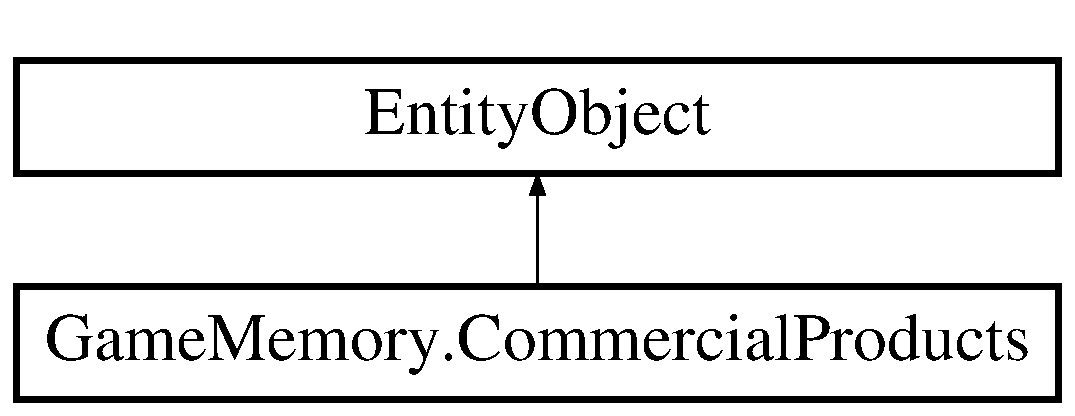
\includegraphics[height=2.000000cm]{class_game_memory_1_1_commercial_products}
\end{center}
\end{figure}
\subsection*{Static Public Member Functions}
\begin{DoxyCompactItemize}
\item 
static \hyperlink{class_game_memory_1_1_commercial_products}{Commercial\-Products} \hyperlink{class_game_memory_1_1_commercial_products_a7281abea1810474d171d7d936bb0069c}{Create\-Commercial\-Products} (global\-::\-System.\-Int32 commercial\-Product\-Id, global\-::\-System.\-Int32 product\-Image\-Id, global\-::\-System.\-Int32 commercial\-Product\-Type\-Id, global\-::\-System.\-Int32 stock, global\-::\-System.\-Int32 customer\-Id)
\begin{DoxyCompactList}\small\item\em Crear un nuevo objeto \hyperlink{class_game_memory_1_1_commercial_products}{Commercial\-Products}. \end{DoxyCompactList}\end{DoxyCompactItemize}
\subsection*{Properties}
\begin{DoxyCompactItemize}
\item 
global\-::\-System.\-Int32 \hyperlink{class_game_memory_1_1_commercial_products_a30bdc23cb928a5a4ffcc46e5cfb6dcbf}{Commercial\-Product\-Id}\hspace{0.3cm}{\ttfamily  \mbox{[}get, set\mbox{]}}
\begin{DoxyCompactList}\small\item\em No hay documentación de metadatos disponible. \end{DoxyCompactList}\item 
global\-::\-System.\-String \hyperlink{class_game_memory_1_1_commercial_products_ac2bea26ba487b163251d3cc2e30f69c6}{Description}\hspace{0.3cm}{\ttfamily  \mbox{[}get, set\mbox{]}}
\begin{DoxyCompactList}\small\item\em No hay documentación de metadatos disponible. \end{DoxyCompactList}\item 
global\-::\-System.\-String \hyperlink{class_game_memory_1_1_commercial_products_a1ecd53e23a0d6730619c832d2baa96a6}{Product\-Name}\hspace{0.3cm}{\ttfamily  \mbox{[}get, set\mbox{]}}
\begin{DoxyCompactList}\small\item\em No hay documentación de metadatos disponible. \end{DoxyCompactList}\item 
global\-::\-System.\-Int32 \hyperlink{class_game_memory_1_1_commercial_products_ab31ea73b3ff3ec456f255b1e215d9147}{Product\-Image\-Id}\hspace{0.3cm}{\ttfamily  \mbox{[}get, set\mbox{]}}
\begin{DoxyCompactList}\small\item\em No hay documentación de metadatos disponible. \end{DoxyCompactList}\item 
global\-::\-System.\-Int32 \hyperlink{class_game_memory_1_1_commercial_products_a0bc077baf7304a4621d25f0d64890148}{Commercial\-Product\-Type\-Id}\hspace{0.3cm}{\ttfamily  \mbox{[}get, set\mbox{]}}
\begin{DoxyCompactList}\small\item\em No hay documentación de metadatos disponible. \end{DoxyCompactList}\item 
global\-::\-System.\-Int32 \hyperlink{class_game_memory_1_1_commercial_products_a647e99bd36a3dc48c7b14fafc499f027}{Stock}\hspace{0.3cm}{\ttfamily  \mbox{[}get, set\mbox{]}}
\begin{DoxyCompactList}\small\item\em No hay documentación de metadatos disponible. \end{DoxyCompactList}\item 
Nullable$<$ global\-::\-System.\-Decimal $>$ \hyperlink{class_game_memory_1_1_commercial_products_a7554ddad0d586549ac0902db89191c08}{Price}\hspace{0.3cm}{\ttfamily  \mbox{[}get, set\mbox{]}}
\begin{DoxyCompactList}\small\item\em No hay documentación de metadatos disponible. \end{DoxyCompactList}\item 
global\-::\-System.\-String \hyperlink{class_game_memory_1_1_commercial_products_a62c8035a92098f4485b3aa532844cfed}{Video\-Path}\hspace{0.3cm}{\ttfamily  \mbox{[}get, set\mbox{]}}
\begin{DoxyCompactList}\small\item\em No hay documentación de metadatos disponible. \end{DoxyCompactList}\item 
global\-::\-System.\-Int32 \hyperlink{class_game_memory_1_1_commercial_products_a25aeb7ff0bac027b1bb5a3a20e359468}{Customer\-Id}\hspace{0.3cm}{\ttfamily  \mbox{[}get, set\mbox{]}}
\begin{DoxyCompactList}\small\item\em No hay documentación de metadatos disponible. \end{DoxyCompactList}\item 
Entity\-Collection$<$ \hyperlink{class_game_memory_1_1_catalog_details}{Catalog\-Details} $>$ \hyperlink{class_game_memory_1_1_commercial_products_ab0650a7e2dfc5f0258442cced8adb818}{Catalog\-Details}\hspace{0.3cm}{\ttfamily  \mbox{[}get, set\mbox{]}}
\begin{DoxyCompactList}\small\item\em No hay documentación de metadatos disponible. \end{DoxyCompactList}\item 
\hyperlink{class_game_memory_1_1_commercial_product_types}{Commercial\-Product\-Types} \hyperlink{class_game_memory_1_1_commercial_products_ac5813dda9f061765d3f1aacb9dda00bf}{Commercial\-Product\-Types}\hspace{0.3cm}{\ttfamily  \mbox{[}get, set\mbox{]}}
\begin{DoxyCompactList}\small\item\em No hay documentación de metadatos disponible. \end{DoxyCompactList}\item 
Entity\-Reference\\*
$<$ \hyperlink{class_game_memory_1_1_commercial_product_types}{Commercial\-Product\-Types} $>$ \hyperlink{class_game_memory_1_1_commercial_products_a57288a4508f92f6aa62dc7402618e8f2}{Commercial\-Product\-Types\-Reference}\hspace{0.3cm}{\ttfamily  \mbox{[}get, set\mbox{]}}
\begin{DoxyCompactList}\small\item\em No hay documentación de metadatos disponible. \end{DoxyCompactList}\item 
\hyperlink{class_game_memory_1_1_customers}{Customers} \hyperlink{class_game_memory_1_1_commercial_products_ad685be3364d165d72cc7312b662c9ce7}{Customers}\hspace{0.3cm}{\ttfamily  \mbox{[}get, set\mbox{]}}
\begin{DoxyCompactList}\small\item\em No hay documentación de metadatos disponible. \end{DoxyCompactList}\item 
Entity\-Reference$<$ \hyperlink{class_game_memory_1_1_customers}{Customers} $>$ \hyperlink{class_game_memory_1_1_commercial_products_ae025504cc119bffe39d2430da20d9ba1}{Customers\-Reference}\hspace{0.3cm}{\ttfamily  \mbox{[}get, set\mbox{]}}
\begin{DoxyCompactList}\small\item\em No hay documentación de metadatos disponible. \end{DoxyCompactList}\item 
\hyperlink{class_game_memory_1_1_product_images}{Product\-Images} \hyperlink{class_game_memory_1_1_commercial_products_ab629e8b21894196949bdae2f5737dd8b}{Product\-Images}\hspace{0.3cm}{\ttfamily  \mbox{[}get, set\mbox{]}}
\begin{DoxyCompactList}\small\item\em No hay documentación de metadatos disponible. \end{DoxyCompactList}\item 
Entity\-Reference$<$ \hyperlink{class_game_memory_1_1_product_images}{Product\-Images} $>$ \hyperlink{class_game_memory_1_1_commercial_products_a2edf86daa617b84658102b4aef34c4b0}{Product\-Images\-Reference}\hspace{0.3cm}{\ttfamily  \mbox{[}get, set\mbox{]}}
\begin{DoxyCompactList}\small\item\em No hay documentación de metadatos disponible. \end{DoxyCompactList}\item 
Entity\-Collection$<$ \hyperlink{class_game_memory_1_1_game_details}{Game\-Details} $>$ \hyperlink{class_game_memory_1_1_commercial_products_a38d43a47cf06ac40a4c45b0a34a3e768}{Game\-Details}\hspace{0.3cm}{\ttfamily  \mbox{[}get, set\mbox{]}}
\begin{DoxyCompactList}\small\item\em No hay documentación de metadatos disponible. \end{DoxyCompactList}\end{DoxyCompactItemize}


\subsection{Detailed Description}
No hay documentación de metadatos disponible. 



\subsection{Member Function Documentation}
\hypertarget{class_game_memory_1_1_commercial_products_a7281abea1810474d171d7d936bb0069c}{\index{Game\-Memory\-::\-Commercial\-Products@{Game\-Memory\-::\-Commercial\-Products}!Create\-Commercial\-Products@{Create\-Commercial\-Products}}
\index{Create\-Commercial\-Products@{Create\-Commercial\-Products}!GameMemory::CommercialProducts@{Game\-Memory\-::\-Commercial\-Products}}
\subsubsection[{Create\-Commercial\-Products}]{\setlength{\rightskip}{0pt plus 5cm}static {\bf Commercial\-Products} Game\-Memory.\-Commercial\-Products.\-Create\-Commercial\-Products (
\begin{DoxyParamCaption}
\item[{global\-::\-System.\-Int32}]{commercial\-Product\-Id, }
\item[{global\-::\-System.\-Int32}]{product\-Image\-Id, }
\item[{global\-::\-System.\-Int32}]{commercial\-Product\-Type\-Id, }
\item[{global\-::\-System.\-Int32}]{stock, }
\item[{global\-::\-System.\-Int32}]{customer\-Id}
\end{DoxyParamCaption}
)\hspace{0.3cm}{\ttfamily [static]}}}\label{class_game_memory_1_1_commercial_products_a7281abea1810474d171d7d936bb0069c}


Crear un nuevo objeto \hyperlink{class_game_memory_1_1_commercial_products}{Commercial\-Products}. 


\begin{DoxyParams}{Parameters}
{\em commercial\-Product\-Id} & Valor inicial de la propiedad Commercial\-Product\-Id.\\
\hline
{\em product\-Image\-Id} & Valor inicial de la propiedad Product\-Image\-Id.\\
\hline
{\em commercial\-Product\-Type\-Id} & Valor inicial de la propiedad Commercial\-Product\-Type\-Id.\\
\hline
{\em stock} & Valor inicial de la propiedad Stock.\\
\hline
{\em customer\-Id} & Valor inicial de la propiedad Customer\-Id.\\
\hline
\end{DoxyParams}


\subsection{Property Documentation}
\hypertarget{class_game_memory_1_1_commercial_products_ab0650a7e2dfc5f0258442cced8adb818}{\index{Game\-Memory\-::\-Commercial\-Products@{Game\-Memory\-::\-Commercial\-Products}!Catalog\-Details@{Catalog\-Details}}
\index{Catalog\-Details@{Catalog\-Details}!GameMemory::CommercialProducts@{Game\-Memory\-::\-Commercial\-Products}}
\subsubsection[{Catalog\-Details}]{\setlength{\rightskip}{0pt plus 5cm}Entity\-Collection$<${\bf Catalog\-Details}$>$ Game\-Memory.\-Commercial\-Products.\-Catalog\-Details\hspace{0.3cm}{\ttfamily [get]}, {\ttfamily [set]}}}\label{class_game_memory_1_1_commercial_products_ab0650a7e2dfc5f0258442cced8adb818}


No hay documentación de metadatos disponible. 

\hypertarget{class_game_memory_1_1_commercial_products_a30bdc23cb928a5a4ffcc46e5cfb6dcbf}{\index{Game\-Memory\-::\-Commercial\-Products@{Game\-Memory\-::\-Commercial\-Products}!Commercial\-Product\-Id@{Commercial\-Product\-Id}}
\index{Commercial\-Product\-Id@{Commercial\-Product\-Id}!GameMemory::CommercialProducts@{Game\-Memory\-::\-Commercial\-Products}}
\subsubsection[{Commercial\-Product\-Id}]{\setlength{\rightskip}{0pt plus 5cm}global.\-System.\-Int32 Game\-Memory.\-Commercial\-Products.\-Commercial\-Product\-Id\hspace{0.3cm}{\ttfamily [get]}, {\ttfamily [set]}}}\label{class_game_memory_1_1_commercial_products_a30bdc23cb928a5a4ffcc46e5cfb6dcbf}


No hay documentación de metadatos disponible. 

\hypertarget{class_game_memory_1_1_commercial_products_a0bc077baf7304a4621d25f0d64890148}{\index{Game\-Memory\-::\-Commercial\-Products@{Game\-Memory\-::\-Commercial\-Products}!Commercial\-Product\-Type\-Id@{Commercial\-Product\-Type\-Id}}
\index{Commercial\-Product\-Type\-Id@{Commercial\-Product\-Type\-Id}!GameMemory::CommercialProducts@{Game\-Memory\-::\-Commercial\-Products}}
\subsubsection[{Commercial\-Product\-Type\-Id}]{\setlength{\rightskip}{0pt plus 5cm}global.\-System.\-Int32 Game\-Memory.\-Commercial\-Products.\-Commercial\-Product\-Type\-Id\hspace{0.3cm}{\ttfamily [get]}, {\ttfamily [set]}}}\label{class_game_memory_1_1_commercial_products_a0bc077baf7304a4621d25f0d64890148}


No hay documentación de metadatos disponible. 

\hypertarget{class_game_memory_1_1_commercial_products_ac5813dda9f061765d3f1aacb9dda00bf}{\index{Game\-Memory\-::\-Commercial\-Products@{Game\-Memory\-::\-Commercial\-Products}!Commercial\-Product\-Types@{Commercial\-Product\-Types}}
\index{Commercial\-Product\-Types@{Commercial\-Product\-Types}!GameMemory::CommercialProducts@{Game\-Memory\-::\-Commercial\-Products}}
\subsubsection[{Commercial\-Product\-Types}]{\setlength{\rightskip}{0pt plus 5cm}{\bf Commercial\-Product\-Types} Game\-Memory.\-Commercial\-Products.\-Commercial\-Product\-Types\hspace{0.3cm}{\ttfamily [get]}, {\ttfamily [set]}}}\label{class_game_memory_1_1_commercial_products_ac5813dda9f061765d3f1aacb9dda00bf}


No hay documentación de metadatos disponible. 

\hypertarget{class_game_memory_1_1_commercial_products_a57288a4508f92f6aa62dc7402618e8f2}{\index{Game\-Memory\-::\-Commercial\-Products@{Game\-Memory\-::\-Commercial\-Products}!Commercial\-Product\-Types\-Reference@{Commercial\-Product\-Types\-Reference}}
\index{Commercial\-Product\-Types\-Reference@{Commercial\-Product\-Types\-Reference}!GameMemory::CommercialProducts@{Game\-Memory\-::\-Commercial\-Products}}
\subsubsection[{Commercial\-Product\-Types\-Reference}]{\setlength{\rightskip}{0pt plus 5cm}Entity\-Reference$<${\bf Commercial\-Product\-Types}$>$ Game\-Memory.\-Commercial\-Products.\-Commercial\-Product\-Types\-Reference\hspace{0.3cm}{\ttfamily [get]}, {\ttfamily [set]}}}\label{class_game_memory_1_1_commercial_products_a57288a4508f92f6aa62dc7402618e8f2}


No hay documentación de metadatos disponible. 

\hypertarget{class_game_memory_1_1_commercial_products_a25aeb7ff0bac027b1bb5a3a20e359468}{\index{Game\-Memory\-::\-Commercial\-Products@{Game\-Memory\-::\-Commercial\-Products}!Customer\-Id@{Customer\-Id}}
\index{Customer\-Id@{Customer\-Id}!GameMemory::CommercialProducts@{Game\-Memory\-::\-Commercial\-Products}}
\subsubsection[{Customer\-Id}]{\setlength{\rightskip}{0pt plus 5cm}global.\-System.\-Int32 Game\-Memory.\-Commercial\-Products.\-Customer\-Id\hspace{0.3cm}{\ttfamily [get]}, {\ttfamily [set]}}}\label{class_game_memory_1_1_commercial_products_a25aeb7ff0bac027b1bb5a3a20e359468}


No hay documentación de metadatos disponible. 

\hypertarget{class_game_memory_1_1_commercial_products_ad685be3364d165d72cc7312b662c9ce7}{\index{Game\-Memory\-::\-Commercial\-Products@{Game\-Memory\-::\-Commercial\-Products}!Customers@{Customers}}
\index{Customers@{Customers}!GameMemory::CommercialProducts@{Game\-Memory\-::\-Commercial\-Products}}
\subsubsection[{Customers}]{\setlength{\rightskip}{0pt plus 5cm}{\bf Customers} Game\-Memory.\-Commercial\-Products.\-Customers\hspace{0.3cm}{\ttfamily [get]}, {\ttfamily [set]}}}\label{class_game_memory_1_1_commercial_products_ad685be3364d165d72cc7312b662c9ce7}


No hay documentación de metadatos disponible. 

\hypertarget{class_game_memory_1_1_commercial_products_ae025504cc119bffe39d2430da20d9ba1}{\index{Game\-Memory\-::\-Commercial\-Products@{Game\-Memory\-::\-Commercial\-Products}!Customers\-Reference@{Customers\-Reference}}
\index{Customers\-Reference@{Customers\-Reference}!GameMemory::CommercialProducts@{Game\-Memory\-::\-Commercial\-Products}}
\subsubsection[{Customers\-Reference}]{\setlength{\rightskip}{0pt plus 5cm}Entity\-Reference$<${\bf Customers}$>$ Game\-Memory.\-Commercial\-Products.\-Customers\-Reference\hspace{0.3cm}{\ttfamily [get]}, {\ttfamily [set]}}}\label{class_game_memory_1_1_commercial_products_ae025504cc119bffe39d2430da20d9ba1}


No hay documentación de metadatos disponible. 

\hypertarget{class_game_memory_1_1_commercial_products_ac2bea26ba487b163251d3cc2e30f69c6}{\index{Game\-Memory\-::\-Commercial\-Products@{Game\-Memory\-::\-Commercial\-Products}!Description@{Description}}
\index{Description@{Description}!GameMemory::CommercialProducts@{Game\-Memory\-::\-Commercial\-Products}}
\subsubsection[{Description}]{\setlength{\rightskip}{0pt plus 5cm}global.\-System.\-String Game\-Memory.\-Commercial\-Products.\-Description\hspace{0.3cm}{\ttfamily [get]}, {\ttfamily [set]}}}\label{class_game_memory_1_1_commercial_products_ac2bea26ba487b163251d3cc2e30f69c6}


No hay documentación de metadatos disponible. 

\hypertarget{class_game_memory_1_1_commercial_products_a38d43a47cf06ac40a4c45b0a34a3e768}{\index{Game\-Memory\-::\-Commercial\-Products@{Game\-Memory\-::\-Commercial\-Products}!Game\-Details@{Game\-Details}}
\index{Game\-Details@{Game\-Details}!GameMemory::CommercialProducts@{Game\-Memory\-::\-Commercial\-Products}}
\subsubsection[{Game\-Details}]{\setlength{\rightskip}{0pt plus 5cm}Entity\-Collection$<${\bf Game\-Details}$>$ Game\-Memory.\-Commercial\-Products.\-Game\-Details\hspace{0.3cm}{\ttfamily [get]}, {\ttfamily [set]}}}\label{class_game_memory_1_1_commercial_products_a38d43a47cf06ac40a4c45b0a34a3e768}


No hay documentación de metadatos disponible. 

\hypertarget{class_game_memory_1_1_commercial_products_a7554ddad0d586549ac0902db89191c08}{\index{Game\-Memory\-::\-Commercial\-Products@{Game\-Memory\-::\-Commercial\-Products}!Price@{Price}}
\index{Price@{Price}!GameMemory::CommercialProducts@{Game\-Memory\-::\-Commercial\-Products}}
\subsubsection[{Price}]{\setlength{\rightskip}{0pt plus 5cm}Nullable$<$global.\-System.\-Decimal$>$ Game\-Memory.\-Commercial\-Products.\-Price\hspace{0.3cm}{\ttfamily [get]}, {\ttfamily [set]}}}\label{class_game_memory_1_1_commercial_products_a7554ddad0d586549ac0902db89191c08}


No hay documentación de metadatos disponible. 

\hypertarget{class_game_memory_1_1_commercial_products_ab31ea73b3ff3ec456f255b1e215d9147}{\index{Game\-Memory\-::\-Commercial\-Products@{Game\-Memory\-::\-Commercial\-Products}!Product\-Image\-Id@{Product\-Image\-Id}}
\index{Product\-Image\-Id@{Product\-Image\-Id}!GameMemory::CommercialProducts@{Game\-Memory\-::\-Commercial\-Products}}
\subsubsection[{Product\-Image\-Id}]{\setlength{\rightskip}{0pt plus 5cm}global.\-System.\-Int32 Game\-Memory.\-Commercial\-Products.\-Product\-Image\-Id\hspace{0.3cm}{\ttfamily [get]}, {\ttfamily [set]}}}\label{class_game_memory_1_1_commercial_products_ab31ea73b3ff3ec456f255b1e215d9147}


No hay documentación de metadatos disponible. 

\hypertarget{class_game_memory_1_1_commercial_products_ab629e8b21894196949bdae2f5737dd8b}{\index{Game\-Memory\-::\-Commercial\-Products@{Game\-Memory\-::\-Commercial\-Products}!Product\-Images@{Product\-Images}}
\index{Product\-Images@{Product\-Images}!GameMemory::CommercialProducts@{Game\-Memory\-::\-Commercial\-Products}}
\subsubsection[{Product\-Images}]{\setlength{\rightskip}{0pt plus 5cm}{\bf Product\-Images} Game\-Memory.\-Commercial\-Products.\-Product\-Images\hspace{0.3cm}{\ttfamily [get]}, {\ttfamily [set]}}}\label{class_game_memory_1_1_commercial_products_ab629e8b21894196949bdae2f5737dd8b}


No hay documentación de metadatos disponible. 

\hypertarget{class_game_memory_1_1_commercial_products_a2edf86daa617b84658102b4aef34c4b0}{\index{Game\-Memory\-::\-Commercial\-Products@{Game\-Memory\-::\-Commercial\-Products}!Product\-Images\-Reference@{Product\-Images\-Reference}}
\index{Product\-Images\-Reference@{Product\-Images\-Reference}!GameMemory::CommercialProducts@{Game\-Memory\-::\-Commercial\-Products}}
\subsubsection[{Product\-Images\-Reference}]{\setlength{\rightskip}{0pt plus 5cm}Entity\-Reference$<${\bf Product\-Images}$>$ Game\-Memory.\-Commercial\-Products.\-Product\-Images\-Reference\hspace{0.3cm}{\ttfamily [get]}, {\ttfamily [set]}}}\label{class_game_memory_1_1_commercial_products_a2edf86daa617b84658102b4aef34c4b0}


No hay documentación de metadatos disponible. 

\hypertarget{class_game_memory_1_1_commercial_products_a1ecd53e23a0d6730619c832d2baa96a6}{\index{Game\-Memory\-::\-Commercial\-Products@{Game\-Memory\-::\-Commercial\-Products}!Product\-Name@{Product\-Name}}
\index{Product\-Name@{Product\-Name}!GameMemory::CommercialProducts@{Game\-Memory\-::\-Commercial\-Products}}
\subsubsection[{Product\-Name}]{\setlength{\rightskip}{0pt plus 5cm}global.\-System.\-String Game\-Memory.\-Commercial\-Products.\-Product\-Name\hspace{0.3cm}{\ttfamily [get]}, {\ttfamily [set]}}}\label{class_game_memory_1_1_commercial_products_a1ecd53e23a0d6730619c832d2baa96a6}


No hay documentación de metadatos disponible. 

\hypertarget{class_game_memory_1_1_commercial_products_a647e99bd36a3dc48c7b14fafc499f027}{\index{Game\-Memory\-::\-Commercial\-Products@{Game\-Memory\-::\-Commercial\-Products}!Stock@{Stock}}
\index{Stock@{Stock}!GameMemory::CommercialProducts@{Game\-Memory\-::\-Commercial\-Products}}
\subsubsection[{Stock}]{\setlength{\rightskip}{0pt plus 5cm}global.\-System.\-Int32 Game\-Memory.\-Commercial\-Products.\-Stock\hspace{0.3cm}{\ttfamily [get]}, {\ttfamily [set]}}}\label{class_game_memory_1_1_commercial_products_a647e99bd36a3dc48c7b14fafc499f027}


No hay documentación de metadatos disponible. 

\hypertarget{class_game_memory_1_1_commercial_products_a62c8035a92098f4485b3aa532844cfed}{\index{Game\-Memory\-::\-Commercial\-Products@{Game\-Memory\-::\-Commercial\-Products}!Video\-Path@{Video\-Path}}
\index{Video\-Path@{Video\-Path}!GameMemory::CommercialProducts@{Game\-Memory\-::\-Commercial\-Products}}
\subsubsection[{Video\-Path}]{\setlength{\rightskip}{0pt plus 5cm}global.\-System.\-String Game\-Memory.\-Commercial\-Products.\-Video\-Path\hspace{0.3cm}{\ttfamily [get]}, {\ttfamily [set]}}}\label{class_game_memory_1_1_commercial_products_a62c8035a92098f4485b3aa532844cfed}


No hay documentación de metadatos disponible. 



The documentation for this class was generated from the following file\-:\begin{DoxyCompactItemize}
\item 
D\-:/tesis\-Assembla/branches/\-Branch\-\_\-\-Tesis\-\_\-\-Sprint01/\-Dev/\-Interaction Module/\-Game\-Memory/\-Game\-Memory/O\-M\-K\-T.\-Designer.\-cs\end{DoxyCompactItemize}

\hypertarget{class_game_memory_1_1_commercial_product_types}{\section{Game\-Memory.\-Commercial\-Product\-Types Class Reference}
\label{class_game_memory_1_1_commercial_product_types}\index{Game\-Memory.\-Commercial\-Product\-Types@{Game\-Memory.\-Commercial\-Product\-Types}}
}


No hay documentación de metadatos disponible.  


Inheritance diagram for Game\-Memory.\-Commercial\-Product\-Types\-:\begin{figure}[H]
\begin{center}
\leavevmode
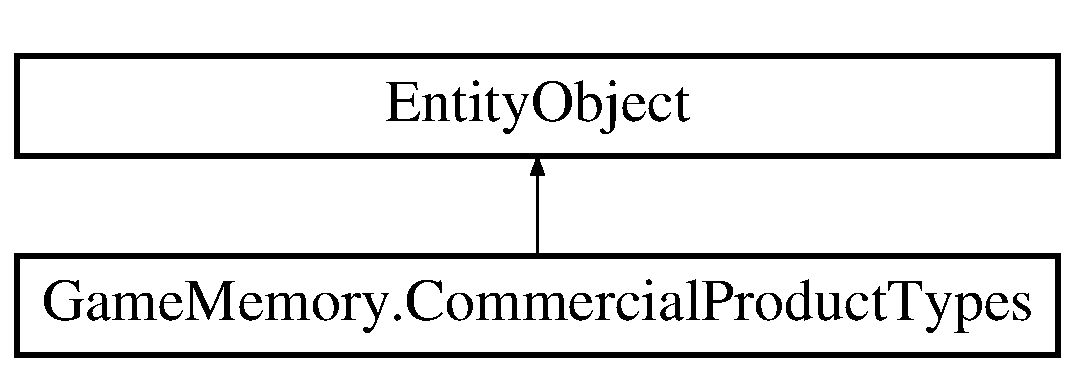
\includegraphics[height=2.000000cm]{class_game_memory_1_1_commercial_product_types}
\end{center}
\end{figure}
\subsection*{Static Public Member Functions}
\begin{DoxyCompactItemize}
\item 
static \hyperlink{class_game_memory_1_1_commercial_product_types}{Commercial\-Product\-Types} \hyperlink{class_game_memory_1_1_commercial_product_types_a5efd99db95615eb5d00bd41dee79dcfd}{Create\-Commercial\-Product\-Types} (global\-::\-System.\-Int32 commercial\-Product\-Type\-Id)
\begin{DoxyCompactList}\small\item\em Crear un nuevo objeto \hyperlink{class_game_memory_1_1_commercial_product_types}{Commercial\-Product\-Types}. \end{DoxyCompactList}\end{DoxyCompactItemize}
\subsection*{Properties}
\begin{DoxyCompactItemize}
\item 
global\-::\-System.\-Int32 \hyperlink{class_game_memory_1_1_commercial_product_types_a259bcdf4dd877d8bae773e9c24bfe00d}{Commercial\-Product\-Type\-Id}\hspace{0.3cm}{\ttfamily  \mbox{[}get, set\mbox{]}}
\begin{DoxyCompactList}\small\item\em No hay documentación de metadatos disponible. \end{DoxyCompactList}\item 
global\-::\-System.\-String \hyperlink{class_game_memory_1_1_commercial_product_types_a299effbd9ebde73b5faea55c63276e12}{Description}\hspace{0.3cm}{\ttfamily  \mbox{[}get, set\mbox{]}}
\begin{DoxyCompactList}\small\item\em No hay documentación de metadatos disponible. \end{DoxyCompactList}\item 
Entity\-Collection\\*
$<$ \hyperlink{class_game_memory_1_1_commercial_products}{Commercial\-Products} $>$ \hyperlink{class_game_memory_1_1_commercial_product_types_ac8c86f5ad74f0123dfeb37b17d83eff1}{Commercial\-Products}\hspace{0.3cm}{\ttfamily  \mbox{[}get, set\mbox{]}}
\begin{DoxyCompactList}\small\item\em No hay documentación de metadatos disponible. \end{DoxyCompactList}\end{DoxyCompactItemize}


\subsection{Detailed Description}
No hay documentación de metadatos disponible. 



\subsection{Member Function Documentation}
\hypertarget{class_game_memory_1_1_commercial_product_types_a5efd99db95615eb5d00bd41dee79dcfd}{\index{Game\-Memory\-::\-Commercial\-Product\-Types@{Game\-Memory\-::\-Commercial\-Product\-Types}!Create\-Commercial\-Product\-Types@{Create\-Commercial\-Product\-Types}}
\index{Create\-Commercial\-Product\-Types@{Create\-Commercial\-Product\-Types}!GameMemory::CommercialProductTypes@{Game\-Memory\-::\-Commercial\-Product\-Types}}
\subsubsection[{Create\-Commercial\-Product\-Types}]{\setlength{\rightskip}{0pt plus 5cm}static {\bf Commercial\-Product\-Types} Game\-Memory.\-Commercial\-Product\-Types.\-Create\-Commercial\-Product\-Types (
\begin{DoxyParamCaption}
\item[{global\-::\-System.\-Int32}]{commercial\-Product\-Type\-Id}
\end{DoxyParamCaption}
)\hspace{0.3cm}{\ttfamily [static]}}}\label{class_game_memory_1_1_commercial_product_types_a5efd99db95615eb5d00bd41dee79dcfd}


Crear un nuevo objeto \hyperlink{class_game_memory_1_1_commercial_product_types}{Commercial\-Product\-Types}. 


\begin{DoxyParams}{Parameters}
{\em commercial\-Product\-Type\-Id} & Valor inicial de la propiedad Commercial\-Product\-Type\-Id.\\
\hline
\end{DoxyParams}


\subsection{Property Documentation}
\hypertarget{class_game_memory_1_1_commercial_product_types_ac8c86f5ad74f0123dfeb37b17d83eff1}{\index{Game\-Memory\-::\-Commercial\-Product\-Types@{Game\-Memory\-::\-Commercial\-Product\-Types}!Commercial\-Products@{Commercial\-Products}}
\index{Commercial\-Products@{Commercial\-Products}!GameMemory::CommercialProductTypes@{Game\-Memory\-::\-Commercial\-Product\-Types}}
\subsubsection[{Commercial\-Products}]{\setlength{\rightskip}{0pt plus 5cm}Entity\-Collection$<${\bf Commercial\-Products}$>$ Game\-Memory.\-Commercial\-Product\-Types.\-Commercial\-Products\hspace{0.3cm}{\ttfamily [get]}, {\ttfamily [set]}}}\label{class_game_memory_1_1_commercial_product_types_ac8c86f5ad74f0123dfeb37b17d83eff1}


No hay documentación de metadatos disponible. 

\hypertarget{class_game_memory_1_1_commercial_product_types_a259bcdf4dd877d8bae773e9c24bfe00d}{\index{Game\-Memory\-::\-Commercial\-Product\-Types@{Game\-Memory\-::\-Commercial\-Product\-Types}!Commercial\-Product\-Type\-Id@{Commercial\-Product\-Type\-Id}}
\index{Commercial\-Product\-Type\-Id@{Commercial\-Product\-Type\-Id}!GameMemory::CommercialProductTypes@{Game\-Memory\-::\-Commercial\-Product\-Types}}
\subsubsection[{Commercial\-Product\-Type\-Id}]{\setlength{\rightskip}{0pt plus 5cm}global.\-System.\-Int32 Game\-Memory.\-Commercial\-Product\-Types.\-Commercial\-Product\-Type\-Id\hspace{0.3cm}{\ttfamily [get]}, {\ttfamily [set]}}}\label{class_game_memory_1_1_commercial_product_types_a259bcdf4dd877d8bae773e9c24bfe00d}


No hay documentación de metadatos disponible. 

\hypertarget{class_game_memory_1_1_commercial_product_types_a299effbd9ebde73b5faea55c63276e12}{\index{Game\-Memory\-::\-Commercial\-Product\-Types@{Game\-Memory\-::\-Commercial\-Product\-Types}!Description@{Description}}
\index{Description@{Description}!GameMemory::CommercialProductTypes@{Game\-Memory\-::\-Commercial\-Product\-Types}}
\subsubsection[{Description}]{\setlength{\rightskip}{0pt plus 5cm}global.\-System.\-String Game\-Memory.\-Commercial\-Product\-Types.\-Description\hspace{0.3cm}{\ttfamily [get]}, {\ttfamily [set]}}}\label{class_game_memory_1_1_commercial_product_types_a299effbd9ebde73b5faea55c63276e12}


No hay documentación de metadatos disponible. 



The documentation for this class was generated from the following file\-:\begin{DoxyCompactItemize}
\item 
D\-:/tesis\-Assembla/branches/\-Branch\-\_\-\-Tesis\-\_\-\-Sprint01/\-Dev/\-Interaction Module/\-Game\-Memory/\-Game\-Memory/O\-M\-K\-T.\-Designer.\-cs\end{DoxyCompactItemize}

\hypertarget{class_game_memory_1_1_customers}{\section{Game\-Memory.\-Customers Class Reference}
\label{class_game_memory_1_1_customers}\index{Game\-Memory.\-Customers@{Game\-Memory.\-Customers}}
}


No hay documentación de metadatos disponible.  


Inheritance diagram for Game\-Memory.\-Customers\-:\begin{figure}[H]
\begin{center}
\leavevmode
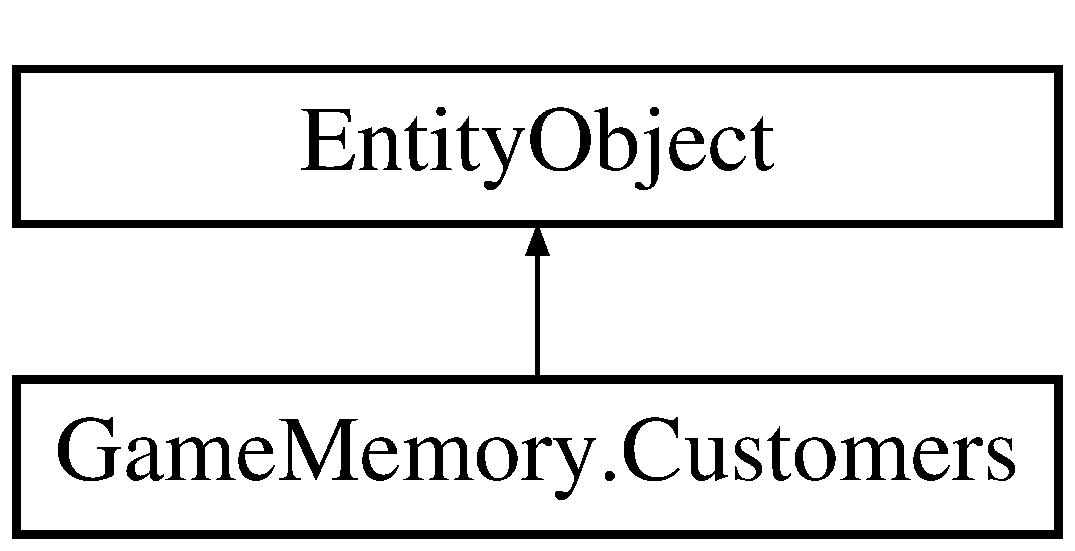
\includegraphics[height=2.000000cm]{class_game_memory_1_1_customers}
\end{center}
\end{figure}
\subsection*{Static Public Member Functions}
\begin{DoxyCompactItemize}
\item 
static \hyperlink{class_game_memory_1_1_customers}{Customers} \hyperlink{class_game_memory_1_1_customers_a7815e50d690b5ce6aa6c1b2dee73ac81}{Create\-Customers} (global\-::\-System.\-Int32 customer\-I\-D, global\-::\-System.\-Boolean is\-Active)
\begin{DoxyCompactList}\small\item\em Crear un nuevo objeto \hyperlink{class_game_memory_1_1_customers}{Customers}. \end{DoxyCompactList}\end{DoxyCompactItemize}
\subsection*{Properties}
\begin{DoxyCompactItemize}
\item 
global\-::\-System.\-Int32 \hyperlink{class_game_memory_1_1_customers_a7b78aa9b1df1d99f6a58dbf25abc0590}{Customer\-I\-D}\hspace{0.3cm}{\ttfamily  \mbox{[}get, set\mbox{]}}
\begin{DoxyCompactList}\small\item\em No hay documentación de metadatos disponible. \end{DoxyCompactList}\item 
global\-::\-System.\-String \hyperlink{class_game_memory_1_1_customers_a12723ccfb832e49e423f8c03b61c5426}{Name}\hspace{0.3cm}{\ttfamily  \mbox{[}get, set\mbox{]}}
\begin{DoxyCompactList}\small\item\em No hay documentación de metadatos disponible. \end{DoxyCompactList}\item 
global\-::\-System.\-String \hyperlink{class_game_memory_1_1_customers_a62e5b08d21d78953b35d3b2fefd833ba}{Company\-Number}\hspace{0.3cm}{\ttfamily  \mbox{[}get, set\mbox{]}}
\begin{DoxyCompactList}\small\item\em No hay documentación de metadatos disponible. \end{DoxyCompactList}\item 
global\-::\-System.\-String \hyperlink{class_game_memory_1_1_customers_a40d18d70faff8547ca6ed5739ae1ae6d}{Address}\hspace{0.3cm}{\ttfamily  \mbox{[}get, set\mbox{]}}
\begin{DoxyCompactList}\small\item\em No hay documentación de metadatos disponible. \end{DoxyCompactList}\item 
global\-::\-System.\-String \hyperlink{class_game_memory_1_1_customers_ad3e8ea3edca56d457e165112a75a27df}{C\-P}\hspace{0.3cm}{\ttfamily  \mbox{[}get, set\mbox{]}}
\begin{DoxyCompactList}\small\item\em No hay documentación de metadatos disponible. \end{DoxyCompactList}\item 
global\-::\-System.\-String \hyperlink{class_game_memory_1_1_customers_adca84dbe266ae65ba70627ec94714276}{City}\hspace{0.3cm}{\ttfamily  \mbox{[}get, set\mbox{]}}
\begin{DoxyCompactList}\small\item\em No hay documentación de metadatos disponible. \end{DoxyCompactList}\item 
global\-::\-System.\-String \hyperlink{class_game_memory_1_1_customers_a3d4d2e80ca8d609a215f4cfe037ccfc0}{Contact\-Person}\hspace{0.3cm}{\ttfamily  \mbox{[}get, set\mbox{]}}
\begin{DoxyCompactList}\small\item\em No hay documentación de metadatos disponible. \end{DoxyCompactList}\item 
global\-::\-System.\-String \hyperlink{class_game_memory_1_1_customers_a0294fbd74c2ccc7636391ecde3a502a1}{Phone1}\hspace{0.3cm}{\ttfamily  \mbox{[}get, set\mbox{]}}
\begin{DoxyCompactList}\small\item\em No hay documentación de metadatos disponible. \end{DoxyCompactList}\item 
global\-::\-System.\-String \hyperlink{class_game_memory_1_1_customers_a6ca17ada64734ee4d301d5bc701ca213}{Phone2}\hspace{0.3cm}{\ttfamily  \mbox{[}get, set\mbox{]}}
\begin{DoxyCompactList}\small\item\em No hay documentación de metadatos disponible. \end{DoxyCompactList}\item 
global\-::\-System.\-Boolean \hyperlink{class_game_memory_1_1_customers_a24e171b530ecc8d281c609bb105e993f}{Is\-Active}\hspace{0.3cm}{\ttfamily  \mbox{[}get, set\mbox{]}}
\begin{DoxyCompactList}\small\item\em No hay documentación de metadatos disponible. \end{DoxyCompactList}\item 
global\-::\-System.\-String \hyperlink{class_game_memory_1_1_customers_a37a6087319b6594adbec2b27b820d0ea}{Email}\hspace{0.3cm}{\ttfamily  \mbox{[}get, set\mbox{]}}
\begin{DoxyCompactList}\small\item\em No hay documentación de metadatos disponible. \end{DoxyCompactList}\item 
Entity\-Collection$<$ \hyperlink{class_game_memory_1_1_advert_campaigns}{Advert\-Campaigns} $>$ \hyperlink{class_game_memory_1_1_customers_ad2341da5ce9ef77380bb9f81aace8ff5}{Advert\-Campaigns}\hspace{0.3cm}{\ttfamily  \mbox{[}get, set\mbox{]}}
\begin{DoxyCompactList}\small\item\em No hay documentación de metadatos disponible. \end{DoxyCompactList}\item 
Entity\-Collection$<$ \hyperlink{class_game_memory_1_1_alerts}{Alerts} $>$ \hyperlink{class_game_memory_1_1_customers_a43d61d4c5dffe15a97d8b48da9a97a19}{Alerts}\hspace{0.3cm}{\ttfamily  \mbox{[}get, set\mbox{]}}
\begin{DoxyCompactList}\small\item\em No hay documentación de metadatos disponible. \end{DoxyCompactList}\item 
Entity\-Collection\\*
$<$ \hyperlink{class_game_memory_1_1_commercial_products}{Commercial\-Products} $>$ \hyperlink{class_game_memory_1_1_customers_af6e416e7fd1236586fab8e29ba132445}{Commercial\-Products}\hspace{0.3cm}{\ttfamily  \mbox{[}get, set\mbox{]}}
\begin{DoxyCompactList}\small\item\em No hay documentación de metadatos disponible. \end{DoxyCompactList}\item 
Entity\-Collection$<$ \hyperlink{class_game_memory_1_1_invoices}{Invoices} $>$ \hyperlink{class_game_memory_1_1_customers_a6348f6d374057879900c399c52a57f02}{Invoices}\hspace{0.3cm}{\ttfamily  \mbox{[}get, set\mbox{]}}
\begin{DoxyCompactList}\small\item\em No hay documentación de metadatos disponible. \end{DoxyCompactList}\item 
Entity\-Collection$<$ \hyperlink{class_game_memory_1_1_users}{Users} $>$ \hyperlink{class_game_memory_1_1_customers_ab53f9e2dc522ccf676bebe8223ccbfdd}{Users}\hspace{0.3cm}{\ttfamily  \mbox{[}get, set\mbox{]}}
\begin{DoxyCompactList}\small\item\em No hay documentación de metadatos disponible. \end{DoxyCompactList}\end{DoxyCompactItemize}


\subsection{Detailed Description}
No hay documentación de metadatos disponible. 



\subsection{Member Function Documentation}
\hypertarget{class_game_memory_1_1_customers_a7815e50d690b5ce6aa6c1b2dee73ac81}{\index{Game\-Memory\-::\-Customers@{Game\-Memory\-::\-Customers}!Create\-Customers@{Create\-Customers}}
\index{Create\-Customers@{Create\-Customers}!GameMemory::Customers@{Game\-Memory\-::\-Customers}}
\subsubsection[{Create\-Customers}]{\setlength{\rightskip}{0pt plus 5cm}static {\bf Customers} Game\-Memory.\-Customers.\-Create\-Customers (
\begin{DoxyParamCaption}
\item[{global\-::\-System.\-Int32}]{customer\-I\-D, }
\item[{global\-::\-System.\-Boolean}]{is\-Active}
\end{DoxyParamCaption}
)\hspace{0.3cm}{\ttfamily [static]}}}\label{class_game_memory_1_1_customers_a7815e50d690b5ce6aa6c1b2dee73ac81}


Crear un nuevo objeto \hyperlink{class_game_memory_1_1_customers}{Customers}. 


\begin{DoxyParams}{Parameters}
{\em customer\-I\-D} & Valor inicial de la propiedad Customer\-I\-D.\\
\hline
{\em is\-Active} & Valor inicial de la propiedad Is\-Active.\\
\hline
\end{DoxyParams}


\subsection{Property Documentation}
\hypertarget{class_game_memory_1_1_customers_a40d18d70faff8547ca6ed5739ae1ae6d}{\index{Game\-Memory\-::\-Customers@{Game\-Memory\-::\-Customers}!Address@{Address}}
\index{Address@{Address}!GameMemory::Customers@{Game\-Memory\-::\-Customers}}
\subsubsection[{Address}]{\setlength{\rightskip}{0pt plus 5cm}global.\-System.\-String Game\-Memory.\-Customers.\-Address\hspace{0.3cm}{\ttfamily [get]}, {\ttfamily [set]}}}\label{class_game_memory_1_1_customers_a40d18d70faff8547ca6ed5739ae1ae6d}


No hay documentación de metadatos disponible. 

\hypertarget{class_game_memory_1_1_customers_ad2341da5ce9ef77380bb9f81aace8ff5}{\index{Game\-Memory\-::\-Customers@{Game\-Memory\-::\-Customers}!Advert\-Campaigns@{Advert\-Campaigns}}
\index{Advert\-Campaigns@{Advert\-Campaigns}!GameMemory::Customers@{Game\-Memory\-::\-Customers}}
\subsubsection[{Advert\-Campaigns}]{\setlength{\rightskip}{0pt plus 5cm}Entity\-Collection$<${\bf Advert\-Campaigns}$>$ Game\-Memory.\-Customers.\-Advert\-Campaigns\hspace{0.3cm}{\ttfamily [get]}, {\ttfamily [set]}}}\label{class_game_memory_1_1_customers_ad2341da5ce9ef77380bb9f81aace8ff5}


No hay documentación de metadatos disponible. 

\hypertarget{class_game_memory_1_1_customers_a43d61d4c5dffe15a97d8b48da9a97a19}{\index{Game\-Memory\-::\-Customers@{Game\-Memory\-::\-Customers}!Alerts@{Alerts}}
\index{Alerts@{Alerts}!GameMemory::Customers@{Game\-Memory\-::\-Customers}}
\subsubsection[{Alerts}]{\setlength{\rightskip}{0pt plus 5cm}Entity\-Collection$<${\bf Alerts}$>$ Game\-Memory.\-Customers.\-Alerts\hspace{0.3cm}{\ttfamily [get]}, {\ttfamily [set]}}}\label{class_game_memory_1_1_customers_a43d61d4c5dffe15a97d8b48da9a97a19}


No hay documentación de metadatos disponible. 

\hypertarget{class_game_memory_1_1_customers_adca84dbe266ae65ba70627ec94714276}{\index{Game\-Memory\-::\-Customers@{Game\-Memory\-::\-Customers}!City@{City}}
\index{City@{City}!GameMemory::Customers@{Game\-Memory\-::\-Customers}}
\subsubsection[{City}]{\setlength{\rightskip}{0pt plus 5cm}global.\-System.\-String Game\-Memory.\-Customers.\-City\hspace{0.3cm}{\ttfamily [get]}, {\ttfamily [set]}}}\label{class_game_memory_1_1_customers_adca84dbe266ae65ba70627ec94714276}


No hay documentación de metadatos disponible. 

\hypertarget{class_game_memory_1_1_customers_af6e416e7fd1236586fab8e29ba132445}{\index{Game\-Memory\-::\-Customers@{Game\-Memory\-::\-Customers}!Commercial\-Products@{Commercial\-Products}}
\index{Commercial\-Products@{Commercial\-Products}!GameMemory::Customers@{Game\-Memory\-::\-Customers}}
\subsubsection[{Commercial\-Products}]{\setlength{\rightskip}{0pt plus 5cm}Entity\-Collection$<${\bf Commercial\-Products}$>$ Game\-Memory.\-Customers.\-Commercial\-Products\hspace{0.3cm}{\ttfamily [get]}, {\ttfamily [set]}}}\label{class_game_memory_1_1_customers_af6e416e7fd1236586fab8e29ba132445}


No hay documentación de metadatos disponible. 

\hypertarget{class_game_memory_1_1_customers_a62e5b08d21d78953b35d3b2fefd833ba}{\index{Game\-Memory\-::\-Customers@{Game\-Memory\-::\-Customers}!Company\-Number@{Company\-Number}}
\index{Company\-Number@{Company\-Number}!GameMemory::Customers@{Game\-Memory\-::\-Customers}}
\subsubsection[{Company\-Number}]{\setlength{\rightskip}{0pt plus 5cm}global.\-System.\-String Game\-Memory.\-Customers.\-Company\-Number\hspace{0.3cm}{\ttfamily [get]}, {\ttfamily [set]}}}\label{class_game_memory_1_1_customers_a62e5b08d21d78953b35d3b2fefd833ba}


No hay documentación de metadatos disponible. 

\hypertarget{class_game_memory_1_1_customers_a3d4d2e80ca8d609a215f4cfe037ccfc0}{\index{Game\-Memory\-::\-Customers@{Game\-Memory\-::\-Customers}!Contact\-Person@{Contact\-Person}}
\index{Contact\-Person@{Contact\-Person}!GameMemory::Customers@{Game\-Memory\-::\-Customers}}
\subsubsection[{Contact\-Person}]{\setlength{\rightskip}{0pt plus 5cm}global.\-System.\-String Game\-Memory.\-Customers.\-Contact\-Person\hspace{0.3cm}{\ttfamily [get]}, {\ttfamily [set]}}}\label{class_game_memory_1_1_customers_a3d4d2e80ca8d609a215f4cfe037ccfc0}


No hay documentación de metadatos disponible. 

\hypertarget{class_game_memory_1_1_customers_ad3e8ea3edca56d457e165112a75a27df}{\index{Game\-Memory\-::\-Customers@{Game\-Memory\-::\-Customers}!C\-P@{C\-P}}
\index{C\-P@{C\-P}!GameMemory::Customers@{Game\-Memory\-::\-Customers}}
\subsubsection[{C\-P}]{\setlength{\rightskip}{0pt plus 5cm}global.\-System.\-String Game\-Memory.\-Customers.\-C\-P\hspace{0.3cm}{\ttfamily [get]}, {\ttfamily [set]}}}\label{class_game_memory_1_1_customers_ad3e8ea3edca56d457e165112a75a27df}


No hay documentación de metadatos disponible. 

\hypertarget{class_game_memory_1_1_customers_a7b78aa9b1df1d99f6a58dbf25abc0590}{\index{Game\-Memory\-::\-Customers@{Game\-Memory\-::\-Customers}!Customer\-I\-D@{Customer\-I\-D}}
\index{Customer\-I\-D@{Customer\-I\-D}!GameMemory::Customers@{Game\-Memory\-::\-Customers}}
\subsubsection[{Customer\-I\-D}]{\setlength{\rightskip}{0pt plus 5cm}global.\-System.\-Int32 Game\-Memory.\-Customers.\-Customer\-I\-D\hspace{0.3cm}{\ttfamily [get]}, {\ttfamily [set]}}}\label{class_game_memory_1_1_customers_a7b78aa9b1df1d99f6a58dbf25abc0590}


No hay documentación de metadatos disponible. 

\hypertarget{class_game_memory_1_1_customers_a37a6087319b6594adbec2b27b820d0ea}{\index{Game\-Memory\-::\-Customers@{Game\-Memory\-::\-Customers}!Email@{Email}}
\index{Email@{Email}!GameMemory::Customers@{Game\-Memory\-::\-Customers}}
\subsubsection[{Email}]{\setlength{\rightskip}{0pt plus 5cm}global.\-System.\-String Game\-Memory.\-Customers.\-Email\hspace{0.3cm}{\ttfamily [get]}, {\ttfamily [set]}}}\label{class_game_memory_1_1_customers_a37a6087319b6594adbec2b27b820d0ea}


No hay documentación de metadatos disponible. 

\hypertarget{class_game_memory_1_1_customers_a6348f6d374057879900c399c52a57f02}{\index{Game\-Memory\-::\-Customers@{Game\-Memory\-::\-Customers}!Invoices@{Invoices}}
\index{Invoices@{Invoices}!GameMemory::Customers@{Game\-Memory\-::\-Customers}}
\subsubsection[{Invoices}]{\setlength{\rightskip}{0pt plus 5cm}Entity\-Collection$<${\bf Invoices}$>$ Game\-Memory.\-Customers.\-Invoices\hspace{0.3cm}{\ttfamily [get]}, {\ttfamily [set]}}}\label{class_game_memory_1_1_customers_a6348f6d374057879900c399c52a57f02}


No hay documentación de metadatos disponible. 

\hypertarget{class_game_memory_1_1_customers_a24e171b530ecc8d281c609bb105e993f}{\index{Game\-Memory\-::\-Customers@{Game\-Memory\-::\-Customers}!Is\-Active@{Is\-Active}}
\index{Is\-Active@{Is\-Active}!GameMemory::Customers@{Game\-Memory\-::\-Customers}}
\subsubsection[{Is\-Active}]{\setlength{\rightskip}{0pt plus 5cm}global.\-System.\-Boolean Game\-Memory.\-Customers.\-Is\-Active\hspace{0.3cm}{\ttfamily [get]}, {\ttfamily [set]}}}\label{class_game_memory_1_1_customers_a24e171b530ecc8d281c609bb105e993f}


No hay documentación de metadatos disponible. 

\hypertarget{class_game_memory_1_1_customers_a12723ccfb832e49e423f8c03b61c5426}{\index{Game\-Memory\-::\-Customers@{Game\-Memory\-::\-Customers}!Name@{Name}}
\index{Name@{Name}!GameMemory::Customers@{Game\-Memory\-::\-Customers}}
\subsubsection[{Name}]{\setlength{\rightskip}{0pt plus 5cm}global.\-System.\-String Game\-Memory.\-Customers.\-Name\hspace{0.3cm}{\ttfamily [get]}, {\ttfamily [set]}}}\label{class_game_memory_1_1_customers_a12723ccfb832e49e423f8c03b61c5426}


No hay documentación de metadatos disponible. 

\hypertarget{class_game_memory_1_1_customers_a0294fbd74c2ccc7636391ecde3a502a1}{\index{Game\-Memory\-::\-Customers@{Game\-Memory\-::\-Customers}!Phone1@{Phone1}}
\index{Phone1@{Phone1}!GameMemory::Customers@{Game\-Memory\-::\-Customers}}
\subsubsection[{Phone1}]{\setlength{\rightskip}{0pt plus 5cm}global.\-System.\-String Game\-Memory.\-Customers.\-Phone1\hspace{0.3cm}{\ttfamily [get]}, {\ttfamily [set]}}}\label{class_game_memory_1_1_customers_a0294fbd74c2ccc7636391ecde3a502a1}


No hay documentación de metadatos disponible. 

\hypertarget{class_game_memory_1_1_customers_a6ca17ada64734ee4d301d5bc701ca213}{\index{Game\-Memory\-::\-Customers@{Game\-Memory\-::\-Customers}!Phone2@{Phone2}}
\index{Phone2@{Phone2}!GameMemory::Customers@{Game\-Memory\-::\-Customers}}
\subsubsection[{Phone2}]{\setlength{\rightskip}{0pt plus 5cm}global.\-System.\-String Game\-Memory.\-Customers.\-Phone2\hspace{0.3cm}{\ttfamily [get]}, {\ttfamily [set]}}}\label{class_game_memory_1_1_customers_a6ca17ada64734ee4d301d5bc701ca213}


No hay documentación de metadatos disponible. 

\hypertarget{class_game_memory_1_1_customers_ab53f9e2dc522ccf676bebe8223ccbfdd}{\index{Game\-Memory\-::\-Customers@{Game\-Memory\-::\-Customers}!Users@{Users}}
\index{Users@{Users}!GameMemory::Customers@{Game\-Memory\-::\-Customers}}
\subsubsection[{Users}]{\setlength{\rightskip}{0pt plus 5cm}Entity\-Collection$<${\bf Users}$>$ Game\-Memory.\-Customers.\-Users\hspace{0.3cm}{\ttfamily [get]}, {\ttfamily [set]}}}\label{class_game_memory_1_1_customers_ab53f9e2dc522ccf676bebe8223ccbfdd}


No hay documentación de metadatos disponible. 



The documentation for this class was generated from the following file\-:\begin{DoxyCompactItemize}
\item 
D\-:/tesis\-Assembla/branches/\-Branch\-\_\-\-Tesis\-\_\-\-Sprint01/\-Dev/\-Interaction Module/\-Game\-Memory/\-Game\-Memory/O\-M\-K\-T.\-Designer.\-cs\end{DoxyCompactItemize}

\hypertarget{class_game_memory_1_1_datos}{\section{Game\-Memory.\-Datos Class Reference}
\label{class_game_memory_1_1_datos}\index{Game\-Memory.\-Datos@{Game\-Memory.\-Datos}}
}
\subsection*{Public Member Functions}
\begin{DoxyCompactItemize}
\item 
\hyperlink{class_game_memory_1_1_adverts}{Adverts} \hyperlink{class_game_memory_1_1_datos_a2e76de0c6baedc5fd26fb4e9ec3eedfe}{Get\-Advert} (String name)
\item 
Boolean \hyperlink{class_game_memory_1_1_datos_aa6db3d4b113ee4a5e2ef447a62a5bb2a}{Update\-Advert\-Campaign\-Interactions} (\hyperlink{class_game_memory_1_1_advert_campaign_interactions}{Advert\-Campaign\-Interactions} advert\-Campaign\-Interactions)
\item 
List$<$ \hyperlink{class_game_memory_1_1_adverts}{Adverts} $>$ \hyperlink{class_game_memory_1_1_datos_a453c1dc1dc586ff3b814857d0d805c0f}{Get\-Adverts} ()
\item 
\hyperlink{class_game_memory_1_1_advert_campaign_interactions}{Advert\-Campaign\-Interactions} \hyperlink{class_game_memory_1_1_datos_a9cd59d07c247460e24e1b8b1db5ead48}{Get\-Advert\-Campaign\-Interactions} ()
\item 
\hyperlink{class_game_memory_1_1_advert_campaign_detail_interactions}{Advert\-Campaign\-Detail\-Interactions} \hyperlink{class_game_memory_1_1_datos_a4acd5b97aef21b73b1162a77d8f34838}{Add\-Advert\-Campaign\-Detail\-Interactions} (\hyperlink{class_game_memory_1_1_advert_campaign_detail_interactions}{Advert\-Campaign\-Detail\-Interactions} advert\-Campaign\-Detail\-Interactions)
\item 
\hyperlink{class_game_memory_1_1_game_detail_interactions}{Game\-Detail\-Interactions} \hyperlink{class_game_memory_1_1_datos_adcf578b5010b961c9f73c40cc27c7f11}{Add\-Game\-Detail\-Interactions} (\hyperlink{class_game_memory_1_1_game_detail_interactions}{Game\-Detail\-Interactions} game\-Detail\-Interactions)
\item 
Boolean \hyperlink{class_game_memory_1_1_datos_a52ac5d5587b844ae7ced3354f9cca896}{Update\-Catalog\-Detail\-Interactions\-All} (Dictionary$<$ String, \hyperlink{class_game_memory_1_1_catalog_detail_interactions}{Catalog\-Detail\-Interactions} $>$ master\-View\-Table)
\item 
Boolean \hyperlink{class_game_memory_1_1_datos_ac68b6adc15b1e3e7402ff8047eb89ab5}{Update\-Advert\-Campaign\-Detail\-Interactions} (\hyperlink{class_game_memory_1_1_advert_campaign_detail_interactions}{Advert\-Campaign\-Detail\-Interactions} advert\-Campaign\-Detail\-Interactions)
\item 
Boolean \hyperlink{class_game_memory_1_1_datos_a6a1820e29422a26a42100e065213d940}{Update\-Game\-Detail\-Interactions} (\hyperlink{class_game_memory_1_1_game_detail_interactions}{Game\-Detail\-Interactions} game\-Detail\-Interactions)
\item 
\hypertarget{class_game_memory_1_1_datos_ac19a3168790816212cbee58c0134efc2}{void {\bfseries Dispose} ()}\label{class_game_memory_1_1_datos_ac19a3168790816212cbee58c0134efc2}

\end{DoxyCompactItemize}


\subsection{Detailed Description}
Clase que controla los datos del Model Entity Framework 

\subsection{Member Function Documentation}
\hypertarget{class_game_memory_1_1_datos_a4acd5b97aef21b73b1162a77d8f34838}{\index{Game\-Memory\-::\-Datos@{Game\-Memory\-::\-Datos}!Add\-Advert\-Campaign\-Detail\-Interactions@{Add\-Advert\-Campaign\-Detail\-Interactions}}
\index{Add\-Advert\-Campaign\-Detail\-Interactions@{Add\-Advert\-Campaign\-Detail\-Interactions}!GameMemory::Datos@{Game\-Memory\-::\-Datos}}
\subsubsection[{Add\-Advert\-Campaign\-Detail\-Interactions}]{\setlength{\rightskip}{0pt plus 5cm}{\bf Advert\-Campaign\-Detail\-Interactions} Game\-Memory.\-Datos.\-Add\-Advert\-Campaign\-Detail\-Interactions (
\begin{DoxyParamCaption}
\item[{{\bf Advert\-Campaign\-Detail\-Interactions}}]{advert\-Campaign\-Detail\-Interactions}
\end{DoxyParamCaption}
)}}\label{class_game_memory_1_1_datos_a4acd5b97aef21b73b1162a77d8f34838}
Method Add\-Advert\-Campaign\-Detail\-Interactions

Agregar un \hyperlink{class_game_memory_1_1_advert_campaign_detail_interactions}{Advert\-Campaign\-Detail\-Interactions} \begin{DoxySince}{Since}
10/06/2013 
\end{DoxySince}

\begin{DoxyParams}{Parameters}
{\em \hyperlink{class_game_memory_1_1_advert_campaign_detail_interactions}{Advert\-Campaign\-Detail\-Interactions},\-:} & objeto \hyperlink{class_game_memory_1_1_advert_campaign_detail_interactions}{Advert\-Campaign\-Detail\-Interactions} a insertar en la base de datos \\
\hline
\end{DoxyParams}
\begin{DoxyReturn}{Returns}
obtengo el \hyperlink{class_game_memory_1_1_advert_campaign_detail_interactions}{Advert\-Campaign\-Detail\-Interactions} con su id 
\end{DoxyReturn}
\hypertarget{class_game_memory_1_1_datos_adcf578b5010b961c9f73c40cc27c7f11}{\index{Game\-Memory\-::\-Datos@{Game\-Memory\-::\-Datos}!Add\-Game\-Detail\-Interactions@{Add\-Game\-Detail\-Interactions}}
\index{Add\-Game\-Detail\-Interactions@{Add\-Game\-Detail\-Interactions}!GameMemory::Datos@{Game\-Memory\-::\-Datos}}
\subsubsection[{Add\-Game\-Detail\-Interactions}]{\setlength{\rightskip}{0pt plus 5cm}{\bf Game\-Detail\-Interactions} Game\-Memory.\-Datos.\-Add\-Game\-Detail\-Interactions (
\begin{DoxyParamCaption}
\item[{{\bf Game\-Detail\-Interactions}}]{game\-Detail\-Interactions}
\end{DoxyParamCaption}
)}}\label{class_game_memory_1_1_datos_adcf578b5010b961c9f73c40cc27c7f11}
method Add\-To\-Game\-Detail\-Interactions Agregar un \hyperlink{class_game_memory_1_1_game_detail_interactions}{Game\-Detail\-Interactions} \begin{DoxySince}{Since}
10/06/2013 
\end{DoxySince}

\begin{DoxyParams}{Parameters}
{\em game\-Detail\-Interactions,\-:} & objeto Add\-To\-Game\-Detail\-Interactions a insertar en la base de datos \\
\hline
\end{DoxyParams}
\begin{DoxyReturn}{Returns}
obtengo el game\-Detail\-Interactions con su id 
\end{DoxyReturn}
\hypertarget{class_game_memory_1_1_datos_a2e76de0c6baedc5fd26fb4e9ec3eedfe}{\index{Game\-Memory\-::\-Datos@{Game\-Memory\-::\-Datos}!Get\-Advert@{Get\-Advert}}
\index{Get\-Advert@{Get\-Advert}!GameMemory::Datos@{Game\-Memory\-::\-Datos}}
\subsubsection[{Get\-Advert}]{\setlength{\rightskip}{0pt plus 5cm}{\bf Adverts} Game\-Memory.\-Datos.\-Get\-Advert (
\begin{DoxyParamCaption}
\item[{String}]{name}
\end{DoxyParamCaption}
)}}\label{class_game_memory_1_1_datos_a2e76de0c6baedc5fd26fb4e9ec3eedfe}
Method Get\-Advert Obtiene un juego espeficado \begin{DoxySince}{Since}
23/07/2013 
\end{DoxySince}

\begin{DoxyParams}{Parameters}
{\em id,\-:} & id del catalogo a obtener \\
\hline
\end{DoxyParams}
\begin{DoxyReturn}{Returns}
Devuelve un objeto \hyperlink{class_game_memory_1_1_adverts}{Adverts} 
\end{DoxyReturn}
\hypertarget{class_game_memory_1_1_datos_a9cd59d07c247460e24e1b8b1db5ead48}{\index{Game\-Memory\-::\-Datos@{Game\-Memory\-::\-Datos}!Get\-Advert\-Campaign\-Interactions@{Get\-Advert\-Campaign\-Interactions}}
\index{Get\-Advert\-Campaign\-Interactions@{Get\-Advert\-Campaign\-Interactions}!GameMemory::Datos@{Game\-Memory\-::\-Datos}}
\subsubsection[{Get\-Advert\-Campaign\-Interactions}]{\setlength{\rightskip}{0pt plus 5cm}{\bf Advert\-Campaign\-Interactions} Game\-Memory.\-Datos.\-Get\-Advert\-Campaign\-Interactions (
\begin{DoxyParamCaption}
{}
\end{DoxyParamCaption}
)}}\label{class_game_memory_1_1_datos_a9cd59d07c247460e24e1b8b1db5ead48}
Method Get\-Advert\-Campaign\-Interactions Obtiene una interacion de campaña \begin{DoxySince}{Since}
23/07/2013 
\end{DoxySince}
\begin{DoxyReturn}{Returns}
Devuelve un objeto \hyperlink{class_game_memory_1_1_advert_campaign_interactions}{Advert\-Campaign\-Interactions} 
\end{DoxyReturn}
\hypertarget{class_game_memory_1_1_datos_a453c1dc1dc586ff3b814857d0d805c0f}{\index{Game\-Memory\-::\-Datos@{Game\-Memory\-::\-Datos}!Get\-Adverts@{Get\-Adverts}}
\index{Get\-Adverts@{Get\-Adverts}!GameMemory::Datos@{Game\-Memory\-::\-Datos}}
\subsubsection[{Get\-Adverts}]{\setlength{\rightskip}{0pt plus 5cm}List$<${\bf Adverts}$>$ Game\-Memory.\-Datos.\-Get\-Adverts (
\begin{DoxyParamCaption}
{}
\end{DoxyParamCaption}
)}}\label{class_game_memory_1_1_datos_a453c1dc1dc586ff3b814857d0d805c0f}
Method Get\-Adverts Obtiene todos los \hyperlink{class_game_memory_1_1_adverts}{Adverts} \begin{DoxySince}{Since}
12/07/2012 
\end{DoxySince}
\begin{DoxyReturn}{Returns}
Devuelve una lista de \hyperlink{class_game_memory_1_1_adverts}{Adverts} 
\end{DoxyReturn}
\hypertarget{class_game_memory_1_1_datos_ac68b6adc15b1e3e7402ff8047eb89ab5}{\index{Game\-Memory\-::\-Datos@{Game\-Memory\-::\-Datos}!Update\-Advert\-Campaign\-Detail\-Interactions@{Update\-Advert\-Campaign\-Detail\-Interactions}}
\index{Update\-Advert\-Campaign\-Detail\-Interactions@{Update\-Advert\-Campaign\-Detail\-Interactions}!GameMemory::Datos@{Game\-Memory\-::\-Datos}}
\subsubsection[{Update\-Advert\-Campaign\-Detail\-Interactions}]{\setlength{\rightskip}{0pt plus 5cm}Boolean Game\-Memory.\-Datos.\-Update\-Advert\-Campaign\-Detail\-Interactions (
\begin{DoxyParamCaption}
\item[{{\bf Advert\-Campaign\-Detail\-Interactions}}]{advert\-Campaign\-Detail\-Interactions}
\end{DoxyParamCaption}
)}}\label{class_game_memory_1_1_datos_ac68b6adc15b1e3e7402ff8047eb89ab5}
Method Update\-Advert\-Campaign\-Detail\-Interactions Actualiza Update\-Advert\-Campaign\-Detail\-Interactions \begin{DoxySince}{Since}
03/07/2013 
\end{DoxySince}

\begin{DoxyParams}{Parameters}
{\em advert\-Campaign\-Detail\-Interactions,\-:} & advert\-Campaign\-Detail\-Interactions actualizar en la base de datos \\
\hline
\end{DoxyParams}
\begin{DoxyReturn}{Returns}
es true si se actualizo exitoxamente 
\end{DoxyReturn}
\hypertarget{class_game_memory_1_1_datos_aa6db3d4b113ee4a5e2ef447a62a5bb2a}{\index{Game\-Memory\-::\-Datos@{Game\-Memory\-::\-Datos}!Update\-Advert\-Campaign\-Interactions@{Update\-Advert\-Campaign\-Interactions}}
\index{Update\-Advert\-Campaign\-Interactions@{Update\-Advert\-Campaign\-Interactions}!GameMemory::Datos@{Game\-Memory\-::\-Datos}}
\subsubsection[{Update\-Advert\-Campaign\-Interactions}]{\setlength{\rightskip}{0pt plus 5cm}Boolean Game\-Memory.\-Datos.\-Update\-Advert\-Campaign\-Interactions (
\begin{DoxyParamCaption}
\item[{{\bf Advert\-Campaign\-Interactions}}]{advert\-Campaign\-Interactions}
\end{DoxyParamCaption}
)}}\label{class_game_memory_1_1_datos_aa6db3d4b113ee4a5e2ef447a62a5bb2a}
Method Update\-Advert\-Campaign\-Detail\-Interactions Actualiza \hyperlink{class_game_memory_1_1_advert_campaign_detail_interactions}{Advert\-Campaign\-Detail\-Interactions} \begin{DoxySince}{Since}
03/07/2013 
\end{DoxySince}

\begin{DoxyParams}{Parameters}
{\em advert\-Campaign\-Detail\-Interactions,\-:} & advert\-Campaign\-Detail\-Interactions actualizar en la base de datos \\
\hline
\end{DoxyParams}
\begin{DoxyReturn}{Returns}
es true si se actualizo exitoxamente 
\end{DoxyReturn}
\hypertarget{class_game_memory_1_1_datos_a52ac5d5587b844ae7ced3354f9cca896}{\index{Game\-Memory\-::\-Datos@{Game\-Memory\-::\-Datos}!Update\-Catalog\-Detail\-Interactions\-All@{Update\-Catalog\-Detail\-Interactions\-All}}
\index{Update\-Catalog\-Detail\-Interactions\-All@{Update\-Catalog\-Detail\-Interactions\-All}!GameMemory::Datos@{Game\-Memory\-::\-Datos}}
\subsubsection[{Update\-Catalog\-Detail\-Interactions\-All}]{\setlength{\rightskip}{0pt plus 5cm}Boolean Game\-Memory.\-Datos.\-Update\-Catalog\-Detail\-Interactions\-All (
\begin{DoxyParamCaption}
\item[{Dictionary$<$ String, {\bf Catalog\-Detail\-Interactions} $>$}]{master\-View\-Table}
\end{DoxyParamCaption}
)}}\label{class_game_memory_1_1_datos_a52ac5d5587b844ae7ced3354f9cca896}
Method Update\-Catalog\-Detail\-Interactions\-All Actualiza todos los Catalog\-Detail\-Interactionss \begin{DoxySince}{Since}
03/07/2013 
\end{DoxySince}

\begin{DoxyParams}{Parameters}
{\em master\-View\-Table,\-:} & Dictionary \hyperlink{class_game_memory_1_1_catalog_detail_interactions}{Catalog\-Detail\-Interactions} a insertar en la base de datos \\
\hline
\end{DoxyParams}
\begin{DoxyReturn}{Returns}
es true si se actualizo exitoxamente 
\end{DoxyReturn}
\hypertarget{class_game_memory_1_1_datos_a6a1820e29422a26a42100e065213d940}{\index{Game\-Memory\-::\-Datos@{Game\-Memory\-::\-Datos}!Update\-Game\-Detail\-Interactions@{Update\-Game\-Detail\-Interactions}}
\index{Update\-Game\-Detail\-Interactions@{Update\-Game\-Detail\-Interactions}!GameMemory::Datos@{Game\-Memory\-::\-Datos}}
\subsubsection[{Update\-Game\-Detail\-Interactions}]{\setlength{\rightskip}{0pt plus 5cm}Boolean Game\-Memory.\-Datos.\-Update\-Game\-Detail\-Interactions (
\begin{DoxyParamCaption}
\item[{{\bf Game\-Detail\-Interactions}}]{game\-Detail\-Interactions}
\end{DoxyParamCaption}
)}}\label{class_game_memory_1_1_datos_a6a1820e29422a26a42100e065213d940}
Method Update\-Game\-Detail\-Interactions Actualiza el game\-Detail\-Interactions \begin{DoxySince}{Since}
03/07/2013 
\end{DoxySince}

\begin{DoxyParams}{Parameters}
{\em game\-Detail\-Interactions,\-:} & \hyperlink{class_game_memory_1_1_game_detail_interactions}{Game\-Detail\-Interactions} a insertar en la base de datos \\
\hline
\end{DoxyParams}
\begin{DoxyReturn}{Returns}
es true si se actualizo exitoxamente 
\end{DoxyReturn}


The documentation for this class was generated from the following file\-:\begin{DoxyCompactItemize}
\item 
D\-:/tesis\-Assembla/branches/\-Branch\-\_\-\-Tesis\-\_\-\-Sprint01/\-Dev/\-Interaction Module/\-Game\-Memory/\-Game\-Memory/Datos.\-cs\end{DoxyCompactItemize}

\hypertarget{class_game_memory_1_1_game_detail_interactions}{\section{Game\-Memory.\-Game\-Detail\-Interactions Class Reference}
\label{class_game_memory_1_1_game_detail_interactions}\index{Game\-Memory.\-Game\-Detail\-Interactions@{Game\-Memory.\-Game\-Detail\-Interactions}}
}


No hay documentación de metadatos disponible.  


Inheritance diagram for Game\-Memory.\-Game\-Detail\-Interactions\-:\begin{figure}[H]
\begin{center}
\leavevmode
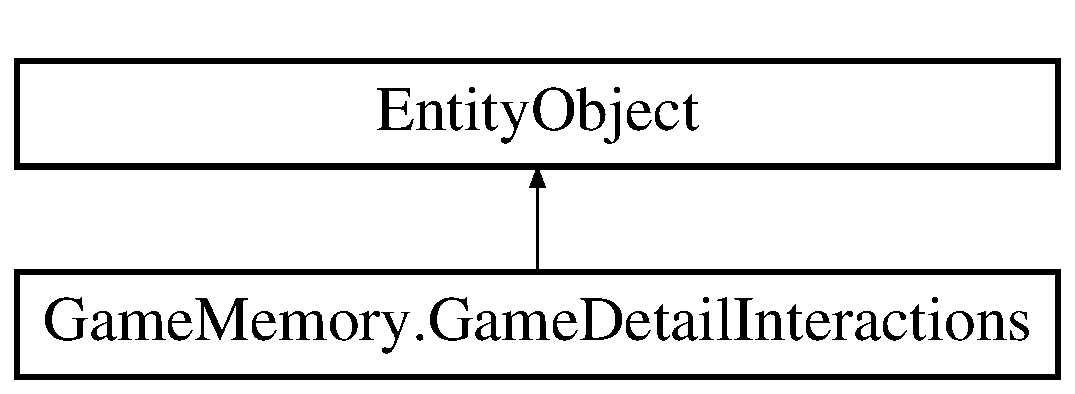
\includegraphics[height=2.000000cm]{class_game_memory_1_1_game_detail_interactions}
\end{center}
\end{figure}
\subsection*{Static Public Member Functions}
\begin{DoxyCompactItemize}
\item 
static \hyperlink{class_game_memory_1_1_game_detail_interactions}{Game\-Detail\-Interactions} \hyperlink{class_game_memory_1_1_game_detail_interactions_a3fb5af1cd91c79675ef646b8e0d6f66b}{Create\-Game\-Detail\-Interactions} (global\-::\-System.\-Int32 game\-Detail\-Interaction\-Id, global\-::\-System.\-Int32 game\-Detail\-I\-D, global\-::\-System.\-Date\-Time start\-Datetime)
\begin{DoxyCompactList}\small\item\em Crear un nuevo objeto \hyperlink{class_game_memory_1_1_game_detail_interactions}{Game\-Detail\-Interactions}. \end{DoxyCompactList}\end{DoxyCompactItemize}
\subsection*{Properties}
\begin{DoxyCompactItemize}
\item 
global\-::\-System.\-Int32 \hyperlink{class_game_memory_1_1_game_detail_interactions_a7c85d9badde12a4e6167757744640f52}{Game\-Detail\-Interaction\-Id}\hspace{0.3cm}{\ttfamily  \mbox{[}get, set\mbox{]}}
\begin{DoxyCompactList}\small\item\em No hay documentación de metadatos disponible. \end{DoxyCompactList}\item 
global\-::\-System.\-Int32 \hyperlink{class_game_memory_1_1_game_detail_interactions_ae1bcee4700f49b55aa0a63ee376d1379}{Game\-Detail\-I\-D}\hspace{0.3cm}{\ttfamily  \mbox{[}get, set\mbox{]}}
\begin{DoxyCompactList}\small\item\em No hay documentación de metadatos disponible. \end{DoxyCompactList}\item 
global\-::\-System.\-Date\-Time \hyperlink{class_game_memory_1_1_game_detail_interactions_a45ccc8af7e045eb3b85e25fda5251ef6}{Start\-Datetime}\hspace{0.3cm}{\ttfamily  \mbox{[}get, set\mbox{]}}
\begin{DoxyCompactList}\small\item\em No hay documentación de metadatos disponible. \end{DoxyCompactList}\item 
Nullable$<$ global\-::\-System.\-Date\-Time $>$ \hyperlink{class_game_memory_1_1_game_detail_interactions_a021bedafc27dc63de5952facb05c6127}{End\-Datetime}\hspace{0.3cm}{\ttfamily  \mbox{[}get, set\mbox{]}}
\begin{DoxyCompactList}\small\item\em No hay documentación de metadatos disponible. \end{DoxyCompactList}\item 
Nullable$<$ global\-::\-System.\-Int32 $>$ \hyperlink{class_game_memory_1_1_game_detail_interactions_a98537a11e123106e4197c9e163fcaa8c}{Time\-Elapsed}\hspace{0.3cm}{\ttfamily  \mbox{[}get, set\mbox{]}}
\begin{DoxyCompactList}\small\item\em No hay documentación de metadatos disponible. \end{DoxyCompactList}\item 
Nullable$<$ global\-::\-System.\-Boolean $>$ \hyperlink{class_game_memory_1_1_game_detail_interactions_aa3afd285fef25ceaf38fe36e2bfb0f6b}{Win}\hspace{0.3cm}{\ttfamily  \mbox{[}get, set\mbox{]}}
\begin{DoxyCompactList}\small\item\em No hay documentación de metadatos disponible. \end{DoxyCompactList}\item 
\hyperlink{class_game_memory_1_1_game_details}{Game\-Details} \hyperlink{class_game_memory_1_1_game_detail_interactions_ac8ae8dbae74af6bdd6c172b0d0b0acf5}{Game\-Details}\hspace{0.3cm}{\ttfamily  \mbox{[}get, set\mbox{]}}
\begin{DoxyCompactList}\small\item\em No hay documentación de metadatos disponible. \end{DoxyCompactList}\item 
Entity\-Reference$<$ \hyperlink{class_game_memory_1_1_game_details}{Game\-Details} $>$ \hyperlink{class_game_memory_1_1_game_detail_interactions_a33a1137aaeec41b55d19507225ed303f}{Game\-Details\-Reference}\hspace{0.3cm}{\ttfamily  \mbox{[}get, set\mbox{]}}
\begin{DoxyCompactList}\small\item\em No hay documentación de metadatos disponible. \end{DoxyCompactList}\end{DoxyCompactItemize}


\subsection{Detailed Description}
No hay documentación de metadatos disponible. 



\subsection{Member Function Documentation}
\hypertarget{class_game_memory_1_1_game_detail_interactions_a3fb5af1cd91c79675ef646b8e0d6f66b}{\index{Game\-Memory\-::\-Game\-Detail\-Interactions@{Game\-Memory\-::\-Game\-Detail\-Interactions}!Create\-Game\-Detail\-Interactions@{Create\-Game\-Detail\-Interactions}}
\index{Create\-Game\-Detail\-Interactions@{Create\-Game\-Detail\-Interactions}!GameMemory::GameDetailInteractions@{Game\-Memory\-::\-Game\-Detail\-Interactions}}
\subsubsection[{Create\-Game\-Detail\-Interactions}]{\setlength{\rightskip}{0pt plus 5cm}static {\bf Game\-Detail\-Interactions} Game\-Memory.\-Game\-Detail\-Interactions.\-Create\-Game\-Detail\-Interactions (
\begin{DoxyParamCaption}
\item[{global\-::\-System.\-Int32}]{game\-Detail\-Interaction\-Id, }
\item[{global\-::\-System.\-Int32}]{game\-Detail\-I\-D, }
\item[{global\-::\-System.\-Date\-Time}]{start\-Datetime}
\end{DoxyParamCaption}
)\hspace{0.3cm}{\ttfamily [static]}}}\label{class_game_memory_1_1_game_detail_interactions_a3fb5af1cd91c79675ef646b8e0d6f66b}


Crear un nuevo objeto \hyperlink{class_game_memory_1_1_game_detail_interactions}{Game\-Detail\-Interactions}. 


\begin{DoxyParams}{Parameters}
{\em game\-Detail\-Interaction\-Id} & Valor inicial de la propiedad Game\-Detail\-Interaction\-Id.\\
\hline
{\em game\-Detail\-I\-D} & Valor inicial de la propiedad Game\-Detail\-I\-D.\\
\hline
{\em start\-Datetime} & Valor inicial de la propiedad Start\-Datetime.\\
\hline
\end{DoxyParams}


\subsection{Property Documentation}
\hypertarget{class_game_memory_1_1_game_detail_interactions_a021bedafc27dc63de5952facb05c6127}{\index{Game\-Memory\-::\-Game\-Detail\-Interactions@{Game\-Memory\-::\-Game\-Detail\-Interactions}!End\-Datetime@{End\-Datetime}}
\index{End\-Datetime@{End\-Datetime}!GameMemory::GameDetailInteractions@{Game\-Memory\-::\-Game\-Detail\-Interactions}}
\subsubsection[{End\-Datetime}]{\setlength{\rightskip}{0pt plus 5cm}Nullable$<$global.\-System.\-Date\-Time$>$ Game\-Memory.\-Game\-Detail\-Interactions.\-End\-Datetime\hspace{0.3cm}{\ttfamily [get]}, {\ttfamily [set]}}}\label{class_game_memory_1_1_game_detail_interactions_a021bedafc27dc63de5952facb05c6127}


No hay documentación de metadatos disponible. 

\hypertarget{class_game_memory_1_1_game_detail_interactions_ae1bcee4700f49b55aa0a63ee376d1379}{\index{Game\-Memory\-::\-Game\-Detail\-Interactions@{Game\-Memory\-::\-Game\-Detail\-Interactions}!Game\-Detail\-I\-D@{Game\-Detail\-I\-D}}
\index{Game\-Detail\-I\-D@{Game\-Detail\-I\-D}!GameMemory::GameDetailInteractions@{Game\-Memory\-::\-Game\-Detail\-Interactions}}
\subsubsection[{Game\-Detail\-I\-D}]{\setlength{\rightskip}{0pt plus 5cm}global.\-System.\-Int32 Game\-Memory.\-Game\-Detail\-Interactions.\-Game\-Detail\-I\-D\hspace{0.3cm}{\ttfamily [get]}, {\ttfamily [set]}}}\label{class_game_memory_1_1_game_detail_interactions_ae1bcee4700f49b55aa0a63ee376d1379}


No hay documentación de metadatos disponible. 

\hypertarget{class_game_memory_1_1_game_detail_interactions_a7c85d9badde12a4e6167757744640f52}{\index{Game\-Memory\-::\-Game\-Detail\-Interactions@{Game\-Memory\-::\-Game\-Detail\-Interactions}!Game\-Detail\-Interaction\-Id@{Game\-Detail\-Interaction\-Id}}
\index{Game\-Detail\-Interaction\-Id@{Game\-Detail\-Interaction\-Id}!GameMemory::GameDetailInteractions@{Game\-Memory\-::\-Game\-Detail\-Interactions}}
\subsubsection[{Game\-Detail\-Interaction\-Id}]{\setlength{\rightskip}{0pt plus 5cm}global.\-System.\-Int32 Game\-Memory.\-Game\-Detail\-Interactions.\-Game\-Detail\-Interaction\-Id\hspace{0.3cm}{\ttfamily [get]}, {\ttfamily [set]}}}\label{class_game_memory_1_1_game_detail_interactions_a7c85d9badde12a4e6167757744640f52}


No hay documentación de metadatos disponible. 

\hypertarget{class_game_memory_1_1_game_detail_interactions_ac8ae8dbae74af6bdd6c172b0d0b0acf5}{\index{Game\-Memory\-::\-Game\-Detail\-Interactions@{Game\-Memory\-::\-Game\-Detail\-Interactions}!Game\-Details@{Game\-Details}}
\index{Game\-Details@{Game\-Details}!GameMemory::GameDetailInteractions@{Game\-Memory\-::\-Game\-Detail\-Interactions}}
\subsubsection[{Game\-Details}]{\setlength{\rightskip}{0pt plus 5cm}{\bf Game\-Details} Game\-Memory.\-Game\-Detail\-Interactions.\-Game\-Details\hspace{0.3cm}{\ttfamily [get]}, {\ttfamily [set]}}}\label{class_game_memory_1_1_game_detail_interactions_ac8ae8dbae74af6bdd6c172b0d0b0acf5}


No hay documentación de metadatos disponible. 

\hypertarget{class_game_memory_1_1_game_detail_interactions_a33a1137aaeec41b55d19507225ed303f}{\index{Game\-Memory\-::\-Game\-Detail\-Interactions@{Game\-Memory\-::\-Game\-Detail\-Interactions}!Game\-Details\-Reference@{Game\-Details\-Reference}}
\index{Game\-Details\-Reference@{Game\-Details\-Reference}!GameMemory::GameDetailInteractions@{Game\-Memory\-::\-Game\-Detail\-Interactions}}
\subsubsection[{Game\-Details\-Reference}]{\setlength{\rightskip}{0pt plus 5cm}Entity\-Reference$<${\bf Game\-Details}$>$ Game\-Memory.\-Game\-Detail\-Interactions.\-Game\-Details\-Reference\hspace{0.3cm}{\ttfamily [get]}, {\ttfamily [set]}}}\label{class_game_memory_1_1_game_detail_interactions_a33a1137aaeec41b55d19507225ed303f}


No hay documentación de metadatos disponible. 

\hypertarget{class_game_memory_1_1_game_detail_interactions_a45ccc8af7e045eb3b85e25fda5251ef6}{\index{Game\-Memory\-::\-Game\-Detail\-Interactions@{Game\-Memory\-::\-Game\-Detail\-Interactions}!Start\-Datetime@{Start\-Datetime}}
\index{Start\-Datetime@{Start\-Datetime}!GameMemory::GameDetailInteractions@{Game\-Memory\-::\-Game\-Detail\-Interactions}}
\subsubsection[{Start\-Datetime}]{\setlength{\rightskip}{0pt plus 5cm}global.\-System.\-Date\-Time Game\-Memory.\-Game\-Detail\-Interactions.\-Start\-Datetime\hspace{0.3cm}{\ttfamily [get]}, {\ttfamily [set]}}}\label{class_game_memory_1_1_game_detail_interactions_a45ccc8af7e045eb3b85e25fda5251ef6}


No hay documentación de metadatos disponible. 

\hypertarget{class_game_memory_1_1_game_detail_interactions_a98537a11e123106e4197c9e163fcaa8c}{\index{Game\-Memory\-::\-Game\-Detail\-Interactions@{Game\-Memory\-::\-Game\-Detail\-Interactions}!Time\-Elapsed@{Time\-Elapsed}}
\index{Time\-Elapsed@{Time\-Elapsed}!GameMemory::GameDetailInteractions@{Game\-Memory\-::\-Game\-Detail\-Interactions}}
\subsubsection[{Time\-Elapsed}]{\setlength{\rightskip}{0pt plus 5cm}Nullable$<$global.\-System.\-Int32$>$ Game\-Memory.\-Game\-Detail\-Interactions.\-Time\-Elapsed\hspace{0.3cm}{\ttfamily [get]}, {\ttfamily [set]}}}\label{class_game_memory_1_1_game_detail_interactions_a98537a11e123106e4197c9e163fcaa8c}


No hay documentación de metadatos disponible. 

\hypertarget{class_game_memory_1_1_game_detail_interactions_aa3afd285fef25ceaf38fe36e2bfb0f6b}{\index{Game\-Memory\-::\-Game\-Detail\-Interactions@{Game\-Memory\-::\-Game\-Detail\-Interactions}!Win@{Win}}
\index{Win@{Win}!GameMemory::GameDetailInteractions@{Game\-Memory\-::\-Game\-Detail\-Interactions}}
\subsubsection[{Win}]{\setlength{\rightskip}{0pt plus 5cm}Nullable$<$global.\-System.\-Boolean$>$ Game\-Memory.\-Game\-Detail\-Interactions.\-Win\hspace{0.3cm}{\ttfamily [get]}, {\ttfamily [set]}}}\label{class_game_memory_1_1_game_detail_interactions_aa3afd285fef25ceaf38fe36e2bfb0f6b}


No hay documentación de metadatos disponible. 



The documentation for this class was generated from the following file\-:\begin{DoxyCompactItemize}
\item 
D\-:/tesis\-Assembla/branches/\-Branch\-\_\-\-Tesis\-\_\-\-Sprint01/\-Dev/\-Interaction Module/\-Game\-Memory/\-Game\-Memory/O\-M\-K\-T.\-Designer.\-cs\end{DoxyCompactItemize}

\hypertarget{class_game_memory_1_1_game_details}{\section{Game\-Memory.\-Game\-Details Class Reference}
\label{class_game_memory_1_1_game_details}\index{Game\-Memory.\-Game\-Details@{Game\-Memory.\-Game\-Details}}
}


No hay documentación de metadatos disponible.  


Inheritance diagram for Game\-Memory.\-Game\-Details\-:\begin{figure}[H]
\begin{center}
\leavevmode
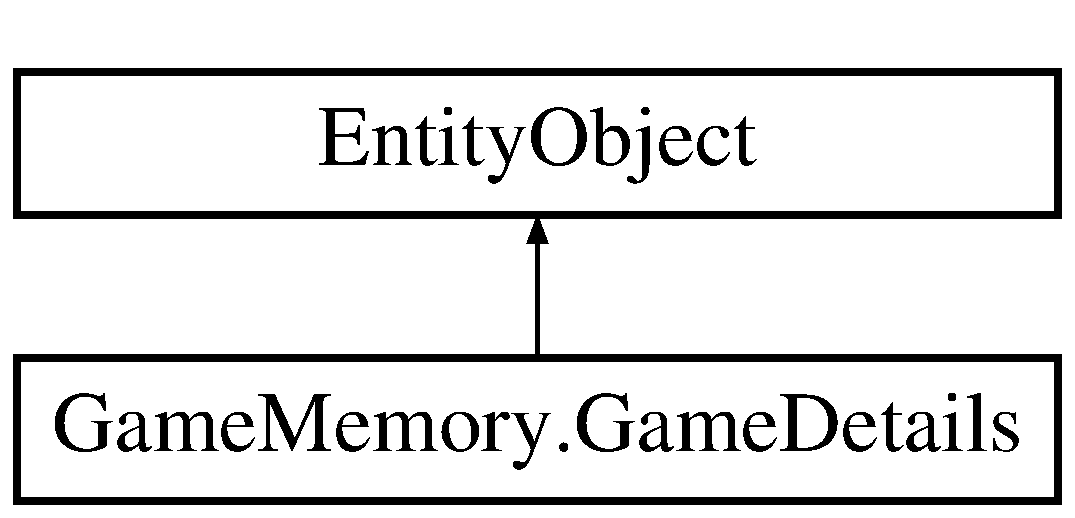
\includegraphics[height=2.000000cm]{class_game_memory_1_1_game_details}
\end{center}
\end{figure}
\subsection*{Static Public Member Functions}
\begin{DoxyCompactItemize}
\item 
static \hyperlink{class_game_memory_1_1_game_details}{Game\-Details} \hyperlink{class_game_memory_1_1_game_details_a0b80aa4ee5ac2a12dd819bf42d46a807}{Create\-Game\-Details} (global\-::\-System.\-Int32 game\-Detail\-Id, global\-::\-System.\-Int32 advert\-Id, global\-::\-System.\-Int32 commercial\-Product\-Id, global\-::\-System.\-Double discount)
\begin{DoxyCompactList}\small\item\em Crear un nuevo objeto \hyperlink{class_game_memory_1_1_game_details}{Game\-Details}. \end{DoxyCompactList}\end{DoxyCompactItemize}
\subsection*{Properties}
\begin{DoxyCompactItemize}
\item 
global\-::\-System.\-Int32 \hyperlink{class_game_memory_1_1_game_details_a18b899c092c351ffb5c98850b8d82103}{Game\-Detail\-Id}\hspace{0.3cm}{\ttfamily  \mbox{[}get, set\mbox{]}}
\begin{DoxyCompactList}\small\item\em No hay documentación de metadatos disponible. \end{DoxyCompactList}\item 
global\-::\-System.\-Int32 \hyperlink{class_game_memory_1_1_game_details_ac1f85d6ae095d852885d3fd88a181106}{Advert\-Id}\hspace{0.3cm}{\ttfamily  \mbox{[}get, set\mbox{]}}
\begin{DoxyCompactList}\small\item\em No hay documentación de metadatos disponible. \end{DoxyCompactList}\item 
global\-::\-System.\-Int32 \hyperlink{class_game_memory_1_1_game_details_a6fdd6c1a3a329df953a5c54a05c260b9}{Commercial\-Product\-Id}\hspace{0.3cm}{\ttfamily  \mbox{[}get, set\mbox{]}}
\begin{DoxyCompactList}\small\item\em No hay documentación de metadatos disponible. \end{DoxyCompactList}\item 
global\-::\-System.\-Double \hyperlink{class_game_memory_1_1_game_details_a1752c3c4d5f63161c372ae8c9742f7fb}{Discount}\hspace{0.3cm}{\ttfamily  \mbox{[}get, set\mbox{]}}
\begin{DoxyCompactList}\small\item\em No hay documentación de metadatos disponible. \end{DoxyCompactList}\item 
global\-::\-System.\-String \hyperlink{class_game_memory_1_1_game_details_ae5cc5d9b422f78685cd588225e4036ac}{Q\-R\-Code}\hspace{0.3cm}{\ttfamily  \mbox{[}get, set\mbox{]}}
\begin{DoxyCompactList}\small\item\em No hay documentación de metadatos disponible. \end{DoxyCompactList}\item 
Nullable$<$ global\-::\-System.\-Date\-Time $>$ \hyperlink{class_game_memory_1_1_game_details_a2d785c106ffd77c7ed2f999bcc6d5749}{Created\-Date}\hspace{0.3cm}{\ttfamily  \mbox{[}get, set\mbox{]}}
\begin{DoxyCompactList}\small\item\em No hay documentación de metadatos disponible. \end{DoxyCompactList}\item 
Nullable$<$ global\-::\-System.\-Date\-Time $>$ \hyperlink{class_game_memory_1_1_game_details_a98363629697ab7b4d13bc4fa5ac7c42b}{Last\-Update}\hspace{0.3cm}{\ttfamily  \mbox{[}get, set\mbox{]}}
\begin{DoxyCompactList}\small\item\em No hay documentación de metadatos disponible. \end{DoxyCompactList}\item 
\hyperlink{class_game_memory_1_1_adverts}{Adverts} \hyperlink{class_game_memory_1_1_game_details_aef99e5d4941a250335738e4ef9f4e9ac}{Adverts}\hspace{0.3cm}{\ttfamily  \mbox{[}get, set\mbox{]}}
\begin{DoxyCompactList}\small\item\em No hay documentación de metadatos disponible. \end{DoxyCompactList}\item 
Entity\-Reference$<$ \hyperlink{class_game_memory_1_1_adverts}{Adverts} $>$ \hyperlink{class_game_memory_1_1_game_details_a52d3aaad97fc57c641ff37f552793da2}{Adverts\-Reference}\hspace{0.3cm}{\ttfamily  \mbox{[}get, set\mbox{]}}
\begin{DoxyCompactList}\small\item\em No hay documentación de metadatos disponible. \end{DoxyCompactList}\item 
\hyperlink{class_game_memory_1_1_commercial_products}{Commercial\-Products} \hyperlink{class_game_memory_1_1_game_details_a030903aaea05ae4b5ab820c6e8fa0fd0}{Commercial\-Products}\hspace{0.3cm}{\ttfamily  \mbox{[}get, set\mbox{]}}
\begin{DoxyCompactList}\small\item\em No hay documentación de metadatos disponible. \end{DoxyCompactList}\item 
Entity\-Reference\\*
$<$ \hyperlink{class_game_memory_1_1_commercial_products}{Commercial\-Products} $>$ \hyperlink{class_game_memory_1_1_game_details_aa3f59a33dd428d393dc3e08585dcff18}{Commercial\-Products\-Reference}\hspace{0.3cm}{\ttfamily  \mbox{[}get, set\mbox{]}}
\begin{DoxyCompactList}\small\item\em No hay documentación de metadatos disponible. \end{DoxyCompactList}\item 
Entity\-Collection\\*
$<$ \hyperlink{class_game_memory_1_1_game_detail_interactions}{Game\-Detail\-Interactions} $>$ \hyperlink{class_game_memory_1_1_game_details_a1faf6b10db4f67fd9bb05ea9a20cf17e}{Game\-Detail\-Interactions}\hspace{0.3cm}{\ttfamily  \mbox{[}get, set\mbox{]}}
\begin{DoxyCompactList}\small\item\em No hay documentación de metadatos disponible. \end{DoxyCompactList}\end{DoxyCompactItemize}


\subsection{Detailed Description}
No hay documentación de metadatos disponible. 



\subsection{Member Function Documentation}
\hypertarget{class_game_memory_1_1_game_details_a0b80aa4ee5ac2a12dd819bf42d46a807}{\index{Game\-Memory\-::\-Game\-Details@{Game\-Memory\-::\-Game\-Details}!Create\-Game\-Details@{Create\-Game\-Details}}
\index{Create\-Game\-Details@{Create\-Game\-Details}!GameMemory::GameDetails@{Game\-Memory\-::\-Game\-Details}}
\subsubsection[{Create\-Game\-Details}]{\setlength{\rightskip}{0pt plus 5cm}static {\bf Game\-Details} Game\-Memory.\-Game\-Details.\-Create\-Game\-Details (
\begin{DoxyParamCaption}
\item[{global\-::\-System.\-Int32}]{game\-Detail\-Id, }
\item[{global\-::\-System.\-Int32}]{advert\-Id, }
\item[{global\-::\-System.\-Int32}]{commercial\-Product\-Id, }
\item[{global\-::\-System.\-Double}]{discount}
\end{DoxyParamCaption}
)\hspace{0.3cm}{\ttfamily [static]}}}\label{class_game_memory_1_1_game_details_a0b80aa4ee5ac2a12dd819bf42d46a807}


Crear un nuevo objeto \hyperlink{class_game_memory_1_1_game_details}{Game\-Details}. 


\begin{DoxyParams}{Parameters}
{\em game\-Detail\-Id} & Valor inicial de la propiedad Game\-Detail\-Id.\\
\hline
{\em advert\-Id} & Valor inicial de la propiedad Advert\-Id.\\
\hline
{\em commercial\-Product\-Id} & Valor inicial de la propiedad Commercial\-Product\-Id.\\
\hline
{\em discount} & Valor inicial de la propiedad Discount.\\
\hline
\end{DoxyParams}


\subsection{Property Documentation}
\hypertarget{class_game_memory_1_1_game_details_ac1f85d6ae095d852885d3fd88a181106}{\index{Game\-Memory\-::\-Game\-Details@{Game\-Memory\-::\-Game\-Details}!Advert\-Id@{Advert\-Id}}
\index{Advert\-Id@{Advert\-Id}!GameMemory::GameDetails@{Game\-Memory\-::\-Game\-Details}}
\subsubsection[{Advert\-Id}]{\setlength{\rightskip}{0pt plus 5cm}global.\-System.\-Int32 Game\-Memory.\-Game\-Details.\-Advert\-Id\hspace{0.3cm}{\ttfamily [get]}, {\ttfamily [set]}}}\label{class_game_memory_1_1_game_details_ac1f85d6ae095d852885d3fd88a181106}


No hay documentación de metadatos disponible. 

\hypertarget{class_game_memory_1_1_game_details_aef99e5d4941a250335738e4ef9f4e9ac}{\index{Game\-Memory\-::\-Game\-Details@{Game\-Memory\-::\-Game\-Details}!Adverts@{Adverts}}
\index{Adverts@{Adverts}!GameMemory::GameDetails@{Game\-Memory\-::\-Game\-Details}}
\subsubsection[{Adverts}]{\setlength{\rightskip}{0pt plus 5cm}{\bf Adverts} Game\-Memory.\-Game\-Details.\-Adverts\hspace{0.3cm}{\ttfamily [get]}, {\ttfamily [set]}}}\label{class_game_memory_1_1_game_details_aef99e5d4941a250335738e4ef9f4e9ac}


No hay documentación de metadatos disponible. 

\hypertarget{class_game_memory_1_1_game_details_a52d3aaad97fc57c641ff37f552793da2}{\index{Game\-Memory\-::\-Game\-Details@{Game\-Memory\-::\-Game\-Details}!Adverts\-Reference@{Adverts\-Reference}}
\index{Adverts\-Reference@{Adverts\-Reference}!GameMemory::GameDetails@{Game\-Memory\-::\-Game\-Details}}
\subsubsection[{Adverts\-Reference}]{\setlength{\rightskip}{0pt plus 5cm}Entity\-Reference$<${\bf Adverts}$>$ Game\-Memory.\-Game\-Details.\-Adverts\-Reference\hspace{0.3cm}{\ttfamily [get]}, {\ttfamily [set]}}}\label{class_game_memory_1_1_game_details_a52d3aaad97fc57c641ff37f552793da2}


No hay documentación de metadatos disponible. 

\hypertarget{class_game_memory_1_1_game_details_a6fdd6c1a3a329df953a5c54a05c260b9}{\index{Game\-Memory\-::\-Game\-Details@{Game\-Memory\-::\-Game\-Details}!Commercial\-Product\-Id@{Commercial\-Product\-Id}}
\index{Commercial\-Product\-Id@{Commercial\-Product\-Id}!GameMemory::GameDetails@{Game\-Memory\-::\-Game\-Details}}
\subsubsection[{Commercial\-Product\-Id}]{\setlength{\rightskip}{0pt plus 5cm}global.\-System.\-Int32 Game\-Memory.\-Game\-Details.\-Commercial\-Product\-Id\hspace{0.3cm}{\ttfamily [get]}, {\ttfamily [set]}}}\label{class_game_memory_1_1_game_details_a6fdd6c1a3a329df953a5c54a05c260b9}


No hay documentación de metadatos disponible. 

\hypertarget{class_game_memory_1_1_game_details_a030903aaea05ae4b5ab820c6e8fa0fd0}{\index{Game\-Memory\-::\-Game\-Details@{Game\-Memory\-::\-Game\-Details}!Commercial\-Products@{Commercial\-Products}}
\index{Commercial\-Products@{Commercial\-Products}!GameMemory::GameDetails@{Game\-Memory\-::\-Game\-Details}}
\subsubsection[{Commercial\-Products}]{\setlength{\rightskip}{0pt plus 5cm}{\bf Commercial\-Products} Game\-Memory.\-Game\-Details.\-Commercial\-Products\hspace{0.3cm}{\ttfamily [get]}, {\ttfamily [set]}}}\label{class_game_memory_1_1_game_details_a030903aaea05ae4b5ab820c6e8fa0fd0}


No hay documentación de metadatos disponible. 

\hypertarget{class_game_memory_1_1_game_details_aa3f59a33dd428d393dc3e08585dcff18}{\index{Game\-Memory\-::\-Game\-Details@{Game\-Memory\-::\-Game\-Details}!Commercial\-Products\-Reference@{Commercial\-Products\-Reference}}
\index{Commercial\-Products\-Reference@{Commercial\-Products\-Reference}!GameMemory::GameDetails@{Game\-Memory\-::\-Game\-Details}}
\subsubsection[{Commercial\-Products\-Reference}]{\setlength{\rightskip}{0pt plus 5cm}Entity\-Reference$<${\bf Commercial\-Products}$>$ Game\-Memory.\-Game\-Details.\-Commercial\-Products\-Reference\hspace{0.3cm}{\ttfamily [get]}, {\ttfamily [set]}}}\label{class_game_memory_1_1_game_details_aa3f59a33dd428d393dc3e08585dcff18}


No hay documentación de metadatos disponible. 

\hypertarget{class_game_memory_1_1_game_details_a2d785c106ffd77c7ed2f999bcc6d5749}{\index{Game\-Memory\-::\-Game\-Details@{Game\-Memory\-::\-Game\-Details}!Created\-Date@{Created\-Date}}
\index{Created\-Date@{Created\-Date}!GameMemory::GameDetails@{Game\-Memory\-::\-Game\-Details}}
\subsubsection[{Created\-Date}]{\setlength{\rightskip}{0pt plus 5cm}Nullable$<$global.\-System.\-Date\-Time$>$ Game\-Memory.\-Game\-Details.\-Created\-Date\hspace{0.3cm}{\ttfamily [get]}, {\ttfamily [set]}}}\label{class_game_memory_1_1_game_details_a2d785c106ffd77c7ed2f999bcc6d5749}


No hay documentación de metadatos disponible. 

\hypertarget{class_game_memory_1_1_game_details_a1752c3c4d5f63161c372ae8c9742f7fb}{\index{Game\-Memory\-::\-Game\-Details@{Game\-Memory\-::\-Game\-Details}!Discount@{Discount}}
\index{Discount@{Discount}!GameMemory::GameDetails@{Game\-Memory\-::\-Game\-Details}}
\subsubsection[{Discount}]{\setlength{\rightskip}{0pt plus 5cm}global.\-System.\-Double Game\-Memory.\-Game\-Details.\-Discount\hspace{0.3cm}{\ttfamily [get]}, {\ttfamily [set]}}}\label{class_game_memory_1_1_game_details_a1752c3c4d5f63161c372ae8c9742f7fb}


No hay documentación de metadatos disponible. 

\hypertarget{class_game_memory_1_1_game_details_a18b899c092c351ffb5c98850b8d82103}{\index{Game\-Memory\-::\-Game\-Details@{Game\-Memory\-::\-Game\-Details}!Game\-Detail\-Id@{Game\-Detail\-Id}}
\index{Game\-Detail\-Id@{Game\-Detail\-Id}!GameMemory::GameDetails@{Game\-Memory\-::\-Game\-Details}}
\subsubsection[{Game\-Detail\-Id}]{\setlength{\rightskip}{0pt plus 5cm}global.\-System.\-Int32 Game\-Memory.\-Game\-Details.\-Game\-Detail\-Id\hspace{0.3cm}{\ttfamily [get]}, {\ttfamily [set]}}}\label{class_game_memory_1_1_game_details_a18b899c092c351ffb5c98850b8d82103}


No hay documentación de metadatos disponible. 

\hypertarget{class_game_memory_1_1_game_details_a1faf6b10db4f67fd9bb05ea9a20cf17e}{\index{Game\-Memory\-::\-Game\-Details@{Game\-Memory\-::\-Game\-Details}!Game\-Detail\-Interactions@{Game\-Detail\-Interactions}}
\index{Game\-Detail\-Interactions@{Game\-Detail\-Interactions}!GameMemory::GameDetails@{Game\-Memory\-::\-Game\-Details}}
\subsubsection[{Game\-Detail\-Interactions}]{\setlength{\rightskip}{0pt plus 5cm}Entity\-Collection$<${\bf Game\-Detail\-Interactions}$>$ Game\-Memory.\-Game\-Details.\-Game\-Detail\-Interactions\hspace{0.3cm}{\ttfamily [get]}, {\ttfamily [set]}}}\label{class_game_memory_1_1_game_details_a1faf6b10db4f67fd9bb05ea9a20cf17e}


No hay documentación de metadatos disponible. 

\hypertarget{class_game_memory_1_1_game_details_a98363629697ab7b4d13bc4fa5ac7c42b}{\index{Game\-Memory\-::\-Game\-Details@{Game\-Memory\-::\-Game\-Details}!Last\-Update@{Last\-Update}}
\index{Last\-Update@{Last\-Update}!GameMemory::GameDetails@{Game\-Memory\-::\-Game\-Details}}
\subsubsection[{Last\-Update}]{\setlength{\rightskip}{0pt plus 5cm}Nullable$<$global.\-System.\-Date\-Time$>$ Game\-Memory.\-Game\-Details.\-Last\-Update\hspace{0.3cm}{\ttfamily [get]}, {\ttfamily [set]}}}\label{class_game_memory_1_1_game_details_a98363629697ab7b4d13bc4fa5ac7c42b}


No hay documentación de metadatos disponible. 

\hypertarget{class_game_memory_1_1_game_details_ae5cc5d9b422f78685cd588225e4036ac}{\index{Game\-Memory\-::\-Game\-Details@{Game\-Memory\-::\-Game\-Details}!Q\-R\-Code@{Q\-R\-Code}}
\index{Q\-R\-Code@{Q\-R\-Code}!GameMemory::GameDetails@{Game\-Memory\-::\-Game\-Details}}
\subsubsection[{Q\-R\-Code}]{\setlength{\rightskip}{0pt plus 5cm}global.\-System.\-String Game\-Memory.\-Game\-Details.\-Q\-R\-Code\hspace{0.3cm}{\ttfamily [get]}, {\ttfamily [set]}}}\label{class_game_memory_1_1_game_details_ae5cc5d9b422f78685cd588225e4036ac}


No hay documentación de metadatos disponible. 



The documentation for this class was generated from the following file\-:\begin{DoxyCompactItemize}
\item 
D\-:/tesis\-Assembla/branches/\-Branch\-\_\-\-Tesis\-\_\-\-Sprint01/\-Dev/\-Interaction Module/\-Game\-Memory/\-Game\-Memory/O\-M\-K\-T.\-Designer.\-cs\end{DoxyCompactItemize}

\hypertarget{class_game_memory_1_1_inboxes}{\section{Game\-Memory.\-Inboxes Class Reference}
\label{class_game_memory_1_1_inboxes}\index{Game\-Memory.\-Inboxes@{Game\-Memory.\-Inboxes}}
}


No hay documentación de metadatos disponible.  


Inheritance diagram for Game\-Memory.\-Inboxes\-:\begin{figure}[H]
\begin{center}
\leavevmode
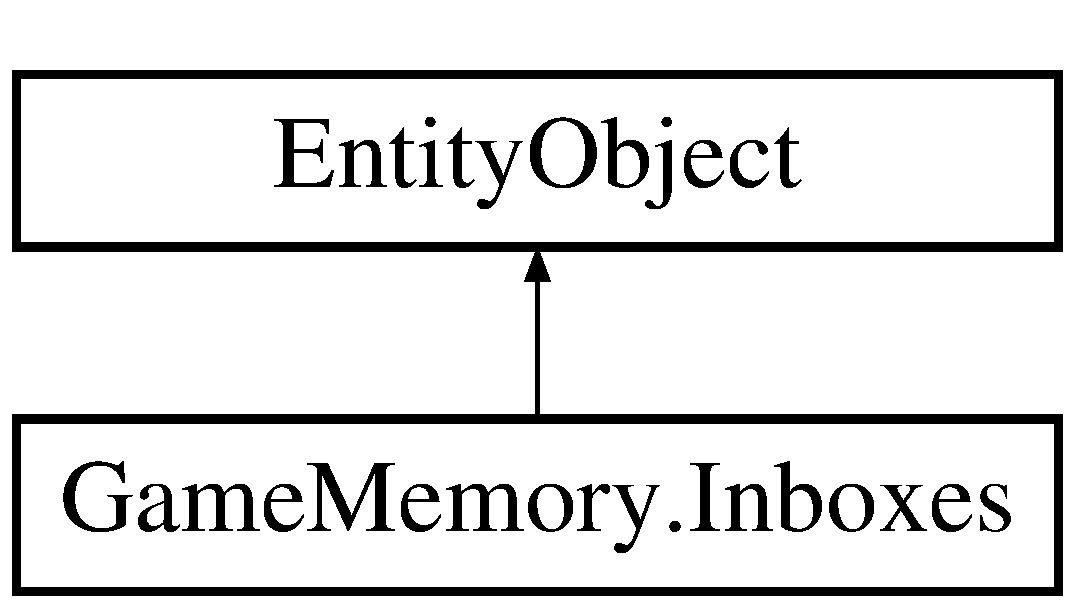
\includegraphics[height=2.000000cm]{class_game_memory_1_1_inboxes}
\end{center}
\end{figure}
\subsection*{Static Public Member Functions}
\begin{DoxyCompactItemize}
\item 
static \hyperlink{class_game_memory_1_1_inboxes}{Inboxes} \hyperlink{class_game_memory_1_1_inboxes_a7bed8cd2f581bd958979c2f46a3c52f5}{Create\-Inboxes} (global\-::\-System.\-Int32 inbox\-Id, global\-::\-System.\-Int32 from\-Id, global\-::\-System.\-Int32 to\-Id, global\-::\-System.\-Boolean unread)
\begin{DoxyCompactList}\small\item\em Crear un nuevo objeto \hyperlink{class_game_memory_1_1_inboxes}{Inboxes}. \end{DoxyCompactList}\end{DoxyCompactItemize}
\subsection*{Properties}
\begin{DoxyCompactItemize}
\item 
global\-::\-System.\-Int32 \hyperlink{class_game_memory_1_1_inboxes_ad8f869d6ea30424629d6ee2e041316fc}{Inbox\-Id}\hspace{0.3cm}{\ttfamily  \mbox{[}get, set\mbox{]}}
\begin{DoxyCompactList}\small\item\em No hay documentación de metadatos disponible. \end{DoxyCompactList}\item 
global\-::\-System.\-String \hyperlink{class_game_memory_1_1_inboxes_ab8eb8f6957620e9bf3d3b18cea3f75f2}{Message}\hspace{0.3cm}{\ttfamily  \mbox{[}get, set\mbox{]}}
\begin{DoxyCompactList}\small\item\em No hay documentación de metadatos disponible. \end{DoxyCompactList}\item 
global\-::\-System.\-Int32 \hyperlink{class_game_memory_1_1_inboxes_af290b883d1ef6a7f31238bc84ee769ed}{From\-Id}\hspace{0.3cm}{\ttfamily  \mbox{[}get, set\mbox{]}}
\begin{DoxyCompactList}\small\item\em No hay documentación de metadatos disponible. \end{DoxyCompactList}\item 
global\-::\-System.\-Int32 \hyperlink{class_game_memory_1_1_inboxes_a198041e29fa5ce1049faf5d86a1adc8d}{To\-Id}\hspace{0.3cm}{\ttfamily  \mbox{[}get, set\mbox{]}}
\begin{DoxyCompactList}\small\item\em No hay documentación de metadatos disponible. \end{DoxyCompactList}\item 
Nullable$<$ global\-::\-System.\-Date\-Time $>$ \hyperlink{class_game_memory_1_1_inboxes_afded22c9818903a94a37984e929150d8}{Timestamp}\hspace{0.3cm}{\ttfamily  \mbox{[}get, set\mbox{]}}
\begin{DoxyCompactList}\small\item\em No hay documentación de metadatos disponible. \end{DoxyCompactList}\item 
global\-::\-System.\-Boolean \hyperlink{class_game_memory_1_1_inboxes_ae67bb69c77c4981be67a1c0f993df287}{Unread}\hspace{0.3cm}{\ttfamily  \mbox{[}get, set\mbox{]}}
\begin{DoxyCompactList}\small\item\em No hay documentación de metadatos disponible. \end{DoxyCompactList}\item 
Nullable$<$ global\-::\-System.\-Guid $>$ \hyperlink{class_game_memory_1_1_inboxes_ae85db34db91880df980eceb08b1a4368}{To\-\_\-\-User\-Id}\hspace{0.3cm}{\ttfamily  \mbox{[}get, set\mbox{]}}
\begin{DoxyCompactList}\small\item\em No hay documentación de metadatos disponible. \end{DoxyCompactList}\item 
\hyperlink{class_game_memory_1_1_users}{Users} \hyperlink{class_game_memory_1_1_inboxes_a5c16a080fdccc957c58acf200f1b52b1}{Users}\hspace{0.3cm}{\ttfamily  \mbox{[}get, set\mbox{]}}
\begin{DoxyCompactList}\small\item\em No hay documentación de metadatos disponible. \end{DoxyCompactList}\item 
Entity\-Reference$<$ \hyperlink{class_game_memory_1_1_users}{Users} $>$ \hyperlink{class_game_memory_1_1_inboxes_a61ad83251581c2d87e830ee9fcfdeb46}{Users\-Reference}\hspace{0.3cm}{\ttfamily  \mbox{[}get, set\mbox{]}}
\begin{DoxyCompactList}\small\item\em No hay documentación de metadatos disponible. \end{DoxyCompactList}\end{DoxyCompactItemize}


\subsection{Detailed Description}
No hay documentación de metadatos disponible. 



\subsection{Member Function Documentation}
\hypertarget{class_game_memory_1_1_inboxes_a7bed8cd2f581bd958979c2f46a3c52f5}{\index{Game\-Memory\-::\-Inboxes@{Game\-Memory\-::\-Inboxes}!Create\-Inboxes@{Create\-Inboxes}}
\index{Create\-Inboxes@{Create\-Inboxes}!GameMemory::Inboxes@{Game\-Memory\-::\-Inboxes}}
\subsubsection[{Create\-Inboxes}]{\setlength{\rightskip}{0pt plus 5cm}static {\bf Inboxes} Game\-Memory.\-Inboxes.\-Create\-Inboxes (
\begin{DoxyParamCaption}
\item[{global\-::\-System.\-Int32}]{inbox\-Id, }
\item[{global\-::\-System.\-Int32}]{from\-Id, }
\item[{global\-::\-System.\-Int32}]{to\-Id, }
\item[{global\-::\-System.\-Boolean}]{unread}
\end{DoxyParamCaption}
)\hspace{0.3cm}{\ttfamily [static]}}}\label{class_game_memory_1_1_inboxes_a7bed8cd2f581bd958979c2f46a3c52f5}


Crear un nuevo objeto \hyperlink{class_game_memory_1_1_inboxes}{Inboxes}. 


\begin{DoxyParams}{Parameters}
{\em inbox\-Id} & Valor inicial de la propiedad Inbox\-Id.\\
\hline
{\em from\-Id} & Valor inicial de la propiedad From\-Id.\\
\hline
{\em to\-Id} & Valor inicial de la propiedad To\-Id.\\
\hline
{\em unread} & Valor inicial de la propiedad Unread.\\
\hline
\end{DoxyParams}


\subsection{Property Documentation}
\hypertarget{class_game_memory_1_1_inboxes_af290b883d1ef6a7f31238bc84ee769ed}{\index{Game\-Memory\-::\-Inboxes@{Game\-Memory\-::\-Inboxes}!From\-Id@{From\-Id}}
\index{From\-Id@{From\-Id}!GameMemory::Inboxes@{Game\-Memory\-::\-Inboxes}}
\subsubsection[{From\-Id}]{\setlength{\rightskip}{0pt plus 5cm}global.\-System.\-Int32 Game\-Memory.\-Inboxes.\-From\-Id\hspace{0.3cm}{\ttfamily [get]}, {\ttfamily [set]}}}\label{class_game_memory_1_1_inboxes_af290b883d1ef6a7f31238bc84ee769ed}


No hay documentación de metadatos disponible. 

\hypertarget{class_game_memory_1_1_inboxes_ad8f869d6ea30424629d6ee2e041316fc}{\index{Game\-Memory\-::\-Inboxes@{Game\-Memory\-::\-Inboxes}!Inbox\-Id@{Inbox\-Id}}
\index{Inbox\-Id@{Inbox\-Id}!GameMemory::Inboxes@{Game\-Memory\-::\-Inboxes}}
\subsubsection[{Inbox\-Id}]{\setlength{\rightskip}{0pt plus 5cm}global.\-System.\-Int32 Game\-Memory.\-Inboxes.\-Inbox\-Id\hspace{0.3cm}{\ttfamily [get]}, {\ttfamily [set]}}}\label{class_game_memory_1_1_inboxes_ad8f869d6ea30424629d6ee2e041316fc}


No hay documentación de metadatos disponible. 

\hypertarget{class_game_memory_1_1_inboxes_ab8eb8f6957620e9bf3d3b18cea3f75f2}{\index{Game\-Memory\-::\-Inboxes@{Game\-Memory\-::\-Inboxes}!Message@{Message}}
\index{Message@{Message}!GameMemory::Inboxes@{Game\-Memory\-::\-Inboxes}}
\subsubsection[{Message}]{\setlength{\rightskip}{0pt plus 5cm}global.\-System.\-String Game\-Memory.\-Inboxes.\-Message\hspace{0.3cm}{\ttfamily [get]}, {\ttfamily [set]}}}\label{class_game_memory_1_1_inboxes_ab8eb8f6957620e9bf3d3b18cea3f75f2}


No hay documentación de metadatos disponible. 

\hypertarget{class_game_memory_1_1_inboxes_afded22c9818903a94a37984e929150d8}{\index{Game\-Memory\-::\-Inboxes@{Game\-Memory\-::\-Inboxes}!Timestamp@{Timestamp}}
\index{Timestamp@{Timestamp}!GameMemory::Inboxes@{Game\-Memory\-::\-Inboxes}}
\subsubsection[{Timestamp}]{\setlength{\rightskip}{0pt plus 5cm}Nullable$<$global.\-System.\-Date\-Time$>$ Game\-Memory.\-Inboxes.\-Timestamp\hspace{0.3cm}{\ttfamily [get]}, {\ttfamily [set]}}}\label{class_game_memory_1_1_inboxes_afded22c9818903a94a37984e929150d8}


No hay documentación de metadatos disponible. 

\hypertarget{class_game_memory_1_1_inboxes_ae85db34db91880df980eceb08b1a4368}{\index{Game\-Memory\-::\-Inboxes@{Game\-Memory\-::\-Inboxes}!To\-\_\-\-User\-Id@{To\-\_\-\-User\-Id}}
\index{To\-\_\-\-User\-Id@{To\-\_\-\-User\-Id}!GameMemory::Inboxes@{Game\-Memory\-::\-Inboxes}}
\subsubsection[{To\-\_\-\-User\-Id}]{\setlength{\rightskip}{0pt plus 5cm}Nullable$<$global.\-System.\-Guid$>$ Game\-Memory.\-Inboxes.\-To\-\_\-\-User\-Id\hspace{0.3cm}{\ttfamily [get]}, {\ttfamily [set]}}}\label{class_game_memory_1_1_inboxes_ae85db34db91880df980eceb08b1a4368}


No hay documentación de metadatos disponible. 

\hypertarget{class_game_memory_1_1_inboxes_a198041e29fa5ce1049faf5d86a1adc8d}{\index{Game\-Memory\-::\-Inboxes@{Game\-Memory\-::\-Inboxes}!To\-Id@{To\-Id}}
\index{To\-Id@{To\-Id}!GameMemory::Inboxes@{Game\-Memory\-::\-Inboxes}}
\subsubsection[{To\-Id}]{\setlength{\rightskip}{0pt plus 5cm}global.\-System.\-Int32 Game\-Memory.\-Inboxes.\-To\-Id\hspace{0.3cm}{\ttfamily [get]}, {\ttfamily [set]}}}\label{class_game_memory_1_1_inboxes_a198041e29fa5ce1049faf5d86a1adc8d}


No hay documentación de metadatos disponible. 

\hypertarget{class_game_memory_1_1_inboxes_ae67bb69c77c4981be67a1c0f993df287}{\index{Game\-Memory\-::\-Inboxes@{Game\-Memory\-::\-Inboxes}!Unread@{Unread}}
\index{Unread@{Unread}!GameMemory::Inboxes@{Game\-Memory\-::\-Inboxes}}
\subsubsection[{Unread}]{\setlength{\rightskip}{0pt plus 5cm}global.\-System.\-Boolean Game\-Memory.\-Inboxes.\-Unread\hspace{0.3cm}{\ttfamily [get]}, {\ttfamily [set]}}}\label{class_game_memory_1_1_inboxes_ae67bb69c77c4981be67a1c0f993df287}


No hay documentación de metadatos disponible. 

\hypertarget{class_game_memory_1_1_inboxes_a5c16a080fdccc957c58acf200f1b52b1}{\index{Game\-Memory\-::\-Inboxes@{Game\-Memory\-::\-Inboxes}!Users@{Users}}
\index{Users@{Users}!GameMemory::Inboxes@{Game\-Memory\-::\-Inboxes}}
\subsubsection[{Users}]{\setlength{\rightskip}{0pt plus 5cm}{\bf Users} Game\-Memory.\-Inboxes.\-Users\hspace{0.3cm}{\ttfamily [get]}, {\ttfamily [set]}}}\label{class_game_memory_1_1_inboxes_a5c16a080fdccc957c58acf200f1b52b1}


No hay documentación de metadatos disponible. 

\hypertarget{class_game_memory_1_1_inboxes_a61ad83251581c2d87e830ee9fcfdeb46}{\index{Game\-Memory\-::\-Inboxes@{Game\-Memory\-::\-Inboxes}!Users\-Reference@{Users\-Reference}}
\index{Users\-Reference@{Users\-Reference}!GameMemory::Inboxes@{Game\-Memory\-::\-Inboxes}}
\subsubsection[{Users\-Reference}]{\setlength{\rightskip}{0pt plus 5cm}Entity\-Reference$<${\bf Users}$>$ Game\-Memory.\-Inboxes.\-Users\-Reference\hspace{0.3cm}{\ttfamily [get]}, {\ttfamily [set]}}}\label{class_game_memory_1_1_inboxes_a61ad83251581c2d87e830ee9fcfdeb46}


No hay documentación de metadatos disponible. 



The documentation for this class was generated from the following file\-:\begin{DoxyCompactItemize}
\item 
D\-:/tesis\-Assembla/branches/\-Branch\-\_\-\-Tesis\-\_\-\-Sprint01/\-Dev/\-Interaction Module/\-Game\-Memory/\-Game\-Memory/O\-M\-K\-T.\-Designer.\-cs\end{DoxyCompactItemize}

\hypertarget{class_game_memory_1_1_interactions}{\section{Game\-Memory.\-Interactions Class Reference}
\label{class_game_memory_1_1_interactions}\index{Game\-Memory.\-Interactions@{Game\-Memory.\-Interactions}}
}


No hay documentación de metadatos disponible.  


Inheritance diagram for Game\-Memory.\-Interactions\-:\begin{figure}[H]
\begin{center}
\leavevmode
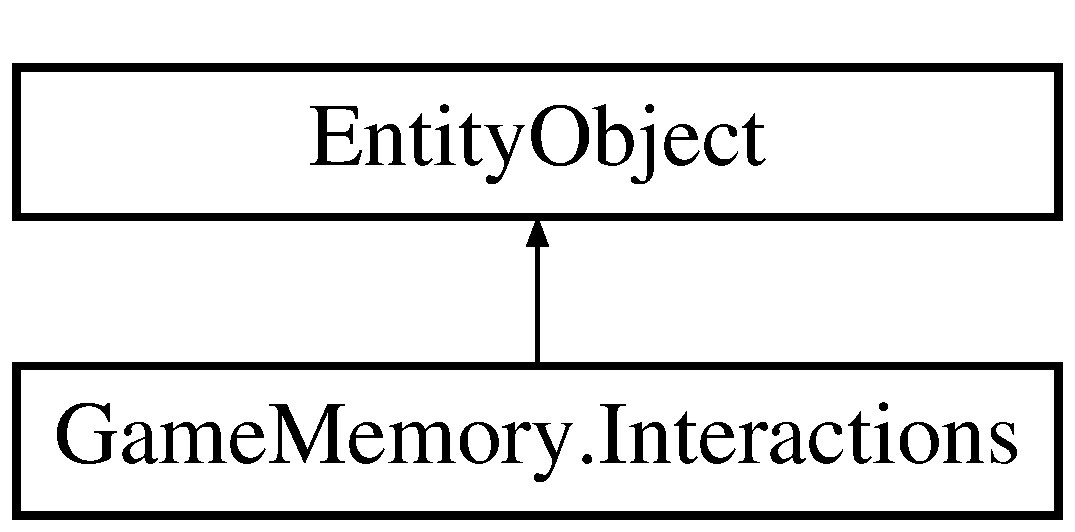
\includegraphics[height=2.000000cm]{class_game_memory_1_1_interactions}
\end{center}
\end{figure}
\subsection*{Static Public Member Functions}
\begin{DoxyCompactItemize}
\item 
static \hyperlink{class_game_memory_1_1_interactions}{Interactions} \hyperlink{class_game_memory_1_1_interactions_a9fb4c4f81722d631a66fbe9587f71336}{Create\-Interactions} (global\-::\-System.\-Int32 interaction\-Id, global\-::\-System.\-Int32 impressions, global\-::\-System.\-Int32 traffic, global\-::\-System.\-Int32 snapshot\-Id)
\begin{DoxyCompactList}\small\item\em Crear un nuevo objeto \hyperlink{class_game_memory_1_1_interactions}{Interactions}. \end{DoxyCompactList}\end{DoxyCompactItemize}
\subsection*{Properties}
\begin{DoxyCompactItemize}
\item 
global\-::\-System.\-Int32 \hyperlink{class_game_memory_1_1_interactions_a1f644eb88ea4634d1760257a2017016a}{Interaction\-Id}\hspace{0.3cm}{\ttfamily  \mbox{[}get, set\mbox{]}}
\begin{DoxyCompactList}\small\item\em No hay documentación de metadatos disponible. \end{DoxyCompactList}\item 
Nullable$<$ global\-::\-System.\-Date\-Time $>$ \hyperlink{class_game_memory_1_1_interactions_adba80b56aece549cdfe01fbe9f618371}{Start\-Date\-Time}\hspace{0.3cm}{\ttfamily  \mbox{[}get, set\mbox{]}}
\begin{DoxyCompactList}\small\item\em No hay documentación de metadatos disponible. \end{DoxyCompactList}\item 
Nullable$<$ global\-::\-System.\-Date\-Time $>$ \hyperlink{class_game_memory_1_1_interactions_a7000d4b58dbf09624957b3868e754dd3}{End\-Date\-Time}\hspace{0.3cm}{\ttfamily  \mbox{[}get, set\mbox{]}}
\begin{DoxyCompactList}\small\item\em No hay documentación de metadatos disponible. \end{DoxyCompactList}\item 
global\-::\-System.\-Int32 \hyperlink{class_game_memory_1_1_interactions_a34268d69790879d63853fb1ab5b72f21}{Impressions}\hspace{0.3cm}{\ttfamily  \mbox{[}get, set\mbox{]}}
\begin{DoxyCompactList}\small\item\em No hay documentación de metadatos disponible. \end{DoxyCompactList}\item 
global\-::\-System.\-Int32 \hyperlink{class_game_memory_1_1_interactions_a3604b151ab46856b0bcb7156476cf279}{Traffic}\hspace{0.3cm}{\ttfamily  \mbox{[}get, set\mbox{]}}
\begin{DoxyCompactList}\small\item\em No hay documentación de metadatos disponible. \end{DoxyCompactList}\item 
global\-::\-System.\-Int32 \hyperlink{class_game_memory_1_1_interactions_a59c14fd2a2ca950b68bed7cfb6f34204}{Snapshot\-Id}\hspace{0.3cm}{\ttfamily  \mbox{[}get, set\mbox{]}}
\begin{DoxyCompactList}\small\item\em No hay documentación de metadatos disponible. \end{DoxyCompactList}\item 
Nullable$<$ global\-::\-System.\-Int32 $>$ \hyperlink{class_game_memory_1_1_interactions_ab8a00140ce65784deb9c0daa8a4d9660}{Advert\-Campaign\-Detail\-\_\-\-Advert\-Campaign\-Detail\-Id}\hspace{0.3cm}{\ttfamily  \mbox{[}get, set\mbox{]}}
\begin{DoxyCompactList}\small\item\em No hay documentación de metadatos disponible. \end{DoxyCompactList}\item 
\hyperlink{class_game_memory_1_1_advert_campaign_details}{Advert\-Campaign\-Details} \hyperlink{class_game_memory_1_1_interactions_a9e244f239f3288b61c5f0defb86e7f61}{Advert\-Campaign\-Details}\hspace{0.3cm}{\ttfamily  \mbox{[}get, set\mbox{]}}
\begin{DoxyCompactList}\small\item\em No hay documentación de metadatos disponible. \end{DoxyCompactList}\item 
Entity\-Reference\\*
$<$ \hyperlink{class_game_memory_1_1_advert_campaign_details}{Advert\-Campaign\-Details} $>$ \hyperlink{class_game_memory_1_1_interactions_ac6192a75df8c0e97efa2f04150e31f7e}{Advert\-Campaign\-Details\-Reference}\hspace{0.3cm}{\ttfamily  \mbox{[}get, set\mbox{]}}
\begin{DoxyCompactList}\small\item\em No hay documentación de metadatos disponible. \end{DoxyCompactList}\item 
\hyperlink{class_game_memory_1_1_snapshots}{Snapshots} \hyperlink{class_game_memory_1_1_interactions_ae86dcc6c95cb31539a33d54cefe4f88d}{Snapshots}\hspace{0.3cm}{\ttfamily  \mbox{[}get, set\mbox{]}}
\begin{DoxyCompactList}\small\item\em No hay documentación de metadatos disponible. \end{DoxyCompactList}\item 
Entity\-Reference$<$ \hyperlink{class_game_memory_1_1_snapshots}{Snapshots} $>$ \hyperlink{class_game_memory_1_1_interactions_a88dffca5092152fbe3917d1e3021a786}{Snapshots\-Reference}\hspace{0.3cm}{\ttfamily  \mbox{[}get, set\mbox{]}}
\begin{DoxyCompactList}\small\item\em No hay documentación de metadatos disponible. \end{DoxyCompactList}\end{DoxyCompactItemize}


\subsection{Detailed Description}
No hay documentación de metadatos disponible. 



\subsection{Member Function Documentation}
\hypertarget{class_game_memory_1_1_interactions_a9fb4c4f81722d631a66fbe9587f71336}{\index{Game\-Memory\-::\-Interactions@{Game\-Memory\-::\-Interactions}!Create\-Interactions@{Create\-Interactions}}
\index{Create\-Interactions@{Create\-Interactions}!GameMemory::Interactions@{Game\-Memory\-::\-Interactions}}
\subsubsection[{Create\-Interactions}]{\setlength{\rightskip}{0pt plus 5cm}static {\bf Interactions} Game\-Memory.\-Interactions.\-Create\-Interactions (
\begin{DoxyParamCaption}
\item[{global\-::\-System.\-Int32}]{interaction\-Id, }
\item[{global\-::\-System.\-Int32}]{impressions, }
\item[{global\-::\-System.\-Int32}]{traffic, }
\item[{global\-::\-System.\-Int32}]{snapshot\-Id}
\end{DoxyParamCaption}
)\hspace{0.3cm}{\ttfamily [static]}}}\label{class_game_memory_1_1_interactions_a9fb4c4f81722d631a66fbe9587f71336}


Crear un nuevo objeto \hyperlink{class_game_memory_1_1_interactions}{Interactions}. 


\begin{DoxyParams}{Parameters}
{\em interaction\-Id} & Valor inicial de la propiedad Interaction\-Id.\\
\hline
{\em impressions} & Valor inicial de la propiedad Impressions.\\
\hline
{\em traffic} & Valor inicial de la propiedad Traffic.\\
\hline
{\em snapshot\-Id} & Valor inicial de la propiedad Snapshot\-Id.\\
\hline
\end{DoxyParams}


\subsection{Property Documentation}
\hypertarget{class_game_memory_1_1_interactions_ab8a00140ce65784deb9c0daa8a4d9660}{\index{Game\-Memory\-::\-Interactions@{Game\-Memory\-::\-Interactions}!Advert\-Campaign\-Detail\-\_\-\-Advert\-Campaign\-Detail\-Id@{Advert\-Campaign\-Detail\-\_\-\-Advert\-Campaign\-Detail\-Id}}
\index{Advert\-Campaign\-Detail\-\_\-\-Advert\-Campaign\-Detail\-Id@{Advert\-Campaign\-Detail\-\_\-\-Advert\-Campaign\-Detail\-Id}!GameMemory::Interactions@{Game\-Memory\-::\-Interactions}}
\subsubsection[{Advert\-Campaign\-Detail\-\_\-\-Advert\-Campaign\-Detail\-Id}]{\setlength{\rightskip}{0pt plus 5cm}Nullable$<$global.\-System.\-Int32$>$ Game\-Memory.\-Interactions.\-Advert\-Campaign\-Detail\-\_\-\-Advert\-Campaign\-Detail\-Id\hspace{0.3cm}{\ttfamily [get]}, {\ttfamily [set]}}}\label{class_game_memory_1_1_interactions_ab8a00140ce65784deb9c0daa8a4d9660}


No hay documentación de metadatos disponible. 

\hypertarget{class_game_memory_1_1_interactions_a9e244f239f3288b61c5f0defb86e7f61}{\index{Game\-Memory\-::\-Interactions@{Game\-Memory\-::\-Interactions}!Advert\-Campaign\-Details@{Advert\-Campaign\-Details}}
\index{Advert\-Campaign\-Details@{Advert\-Campaign\-Details}!GameMemory::Interactions@{Game\-Memory\-::\-Interactions}}
\subsubsection[{Advert\-Campaign\-Details}]{\setlength{\rightskip}{0pt plus 5cm}{\bf Advert\-Campaign\-Details} Game\-Memory.\-Interactions.\-Advert\-Campaign\-Details\hspace{0.3cm}{\ttfamily [get]}, {\ttfamily [set]}}}\label{class_game_memory_1_1_interactions_a9e244f239f3288b61c5f0defb86e7f61}


No hay documentación de metadatos disponible. 

\hypertarget{class_game_memory_1_1_interactions_ac6192a75df8c0e97efa2f04150e31f7e}{\index{Game\-Memory\-::\-Interactions@{Game\-Memory\-::\-Interactions}!Advert\-Campaign\-Details\-Reference@{Advert\-Campaign\-Details\-Reference}}
\index{Advert\-Campaign\-Details\-Reference@{Advert\-Campaign\-Details\-Reference}!GameMemory::Interactions@{Game\-Memory\-::\-Interactions}}
\subsubsection[{Advert\-Campaign\-Details\-Reference}]{\setlength{\rightskip}{0pt plus 5cm}Entity\-Reference$<${\bf Advert\-Campaign\-Details}$>$ Game\-Memory.\-Interactions.\-Advert\-Campaign\-Details\-Reference\hspace{0.3cm}{\ttfamily [get]}, {\ttfamily [set]}}}\label{class_game_memory_1_1_interactions_ac6192a75df8c0e97efa2f04150e31f7e}


No hay documentación de metadatos disponible. 

\hypertarget{class_game_memory_1_1_interactions_a7000d4b58dbf09624957b3868e754dd3}{\index{Game\-Memory\-::\-Interactions@{Game\-Memory\-::\-Interactions}!End\-Date\-Time@{End\-Date\-Time}}
\index{End\-Date\-Time@{End\-Date\-Time}!GameMemory::Interactions@{Game\-Memory\-::\-Interactions}}
\subsubsection[{End\-Date\-Time}]{\setlength{\rightskip}{0pt plus 5cm}Nullable$<$global.\-System.\-Date\-Time$>$ Game\-Memory.\-Interactions.\-End\-Date\-Time\hspace{0.3cm}{\ttfamily [get]}, {\ttfamily [set]}}}\label{class_game_memory_1_1_interactions_a7000d4b58dbf09624957b3868e754dd3}


No hay documentación de metadatos disponible. 

\hypertarget{class_game_memory_1_1_interactions_a34268d69790879d63853fb1ab5b72f21}{\index{Game\-Memory\-::\-Interactions@{Game\-Memory\-::\-Interactions}!Impressions@{Impressions}}
\index{Impressions@{Impressions}!GameMemory::Interactions@{Game\-Memory\-::\-Interactions}}
\subsubsection[{Impressions}]{\setlength{\rightskip}{0pt plus 5cm}global.\-System.\-Int32 Game\-Memory.\-Interactions.\-Impressions\hspace{0.3cm}{\ttfamily [get]}, {\ttfamily [set]}}}\label{class_game_memory_1_1_interactions_a34268d69790879d63853fb1ab5b72f21}


No hay documentación de metadatos disponible. 

\hypertarget{class_game_memory_1_1_interactions_a1f644eb88ea4634d1760257a2017016a}{\index{Game\-Memory\-::\-Interactions@{Game\-Memory\-::\-Interactions}!Interaction\-Id@{Interaction\-Id}}
\index{Interaction\-Id@{Interaction\-Id}!GameMemory::Interactions@{Game\-Memory\-::\-Interactions}}
\subsubsection[{Interaction\-Id}]{\setlength{\rightskip}{0pt plus 5cm}global.\-System.\-Int32 Game\-Memory.\-Interactions.\-Interaction\-Id\hspace{0.3cm}{\ttfamily [get]}, {\ttfamily [set]}}}\label{class_game_memory_1_1_interactions_a1f644eb88ea4634d1760257a2017016a}


No hay documentación de metadatos disponible. 

\hypertarget{class_game_memory_1_1_interactions_a59c14fd2a2ca950b68bed7cfb6f34204}{\index{Game\-Memory\-::\-Interactions@{Game\-Memory\-::\-Interactions}!Snapshot\-Id@{Snapshot\-Id}}
\index{Snapshot\-Id@{Snapshot\-Id}!GameMemory::Interactions@{Game\-Memory\-::\-Interactions}}
\subsubsection[{Snapshot\-Id}]{\setlength{\rightskip}{0pt plus 5cm}global.\-System.\-Int32 Game\-Memory.\-Interactions.\-Snapshot\-Id\hspace{0.3cm}{\ttfamily [get]}, {\ttfamily [set]}}}\label{class_game_memory_1_1_interactions_a59c14fd2a2ca950b68bed7cfb6f34204}


No hay documentación de metadatos disponible. 

\hypertarget{class_game_memory_1_1_interactions_ae86dcc6c95cb31539a33d54cefe4f88d}{\index{Game\-Memory\-::\-Interactions@{Game\-Memory\-::\-Interactions}!Snapshots@{Snapshots}}
\index{Snapshots@{Snapshots}!GameMemory::Interactions@{Game\-Memory\-::\-Interactions}}
\subsubsection[{Snapshots}]{\setlength{\rightskip}{0pt plus 5cm}{\bf Snapshots} Game\-Memory.\-Interactions.\-Snapshots\hspace{0.3cm}{\ttfamily [get]}, {\ttfamily [set]}}}\label{class_game_memory_1_1_interactions_ae86dcc6c95cb31539a33d54cefe4f88d}


No hay documentación de metadatos disponible. 

\hypertarget{class_game_memory_1_1_interactions_a88dffca5092152fbe3917d1e3021a786}{\index{Game\-Memory\-::\-Interactions@{Game\-Memory\-::\-Interactions}!Snapshots\-Reference@{Snapshots\-Reference}}
\index{Snapshots\-Reference@{Snapshots\-Reference}!GameMemory::Interactions@{Game\-Memory\-::\-Interactions}}
\subsubsection[{Snapshots\-Reference}]{\setlength{\rightskip}{0pt plus 5cm}Entity\-Reference$<${\bf Snapshots}$>$ Game\-Memory.\-Interactions.\-Snapshots\-Reference\hspace{0.3cm}{\ttfamily [get]}, {\ttfamily [set]}}}\label{class_game_memory_1_1_interactions_a88dffca5092152fbe3917d1e3021a786}


No hay documentación de metadatos disponible. 

\hypertarget{class_game_memory_1_1_interactions_adba80b56aece549cdfe01fbe9f618371}{\index{Game\-Memory\-::\-Interactions@{Game\-Memory\-::\-Interactions}!Start\-Date\-Time@{Start\-Date\-Time}}
\index{Start\-Date\-Time@{Start\-Date\-Time}!GameMemory::Interactions@{Game\-Memory\-::\-Interactions}}
\subsubsection[{Start\-Date\-Time}]{\setlength{\rightskip}{0pt plus 5cm}Nullable$<$global.\-System.\-Date\-Time$>$ Game\-Memory.\-Interactions.\-Start\-Date\-Time\hspace{0.3cm}{\ttfamily [get]}, {\ttfamily [set]}}}\label{class_game_memory_1_1_interactions_adba80b56aece549cdfe01fbe9f618371}


No hay documentación de metadatos disponible. 

\hypertarget{class_game_memory_1_1_interactions_a3604b151ab46856b0bcb7156476cf279}{\index{Game\-Memory\-::\-Interactions@{Game\-Memory\-::\-Interactions}!Traffic@{Traffic}}
\index{Traffic@{Traffic}!GameMemory::Interactions@{Game\-Memory\-::\-Interactions}}
\subsubsection[{Traffic}]{\setlength{\rightskip}{0pt plus 5cm}global.\-System.\-Int32 Game\-Memory.\-Interactions.\-Traffic\hspace{0.3cm}{\ttfamily [get]}, {\ttfamily [set]}}}\label{class_game_memory_1_1_interactions_a3604b151ab46856b0bcb7156476cf279}


No hay documentación de metadatos disponible. 



The documentation for this class was generated from the following file\-:\begin{DoxyCompactItemize}
\item 
D\-:/tesis\-Assembla/branches/\-Branch\-\_\-\-Tesis\-\_\-\-Sprint01/\-Dev/\-Interaction Module/\-Game\-Memory/\-Game\-Memory/O\-M\-K\-T.\-Designer.\-cs\end{DoxyCompactItemize}

\hypertarget{class_game_memory_1_1_invoice_details}{\section{Game\-Memory.\-Invoice\-Details Class Reference}
\label{class_game_memory_1_1_invoice_details}\index{Game\-Memory.\-Invoice\-Details@{Game\-Memory.\-Invoice\-Details}}
}


No hay documentación de metadatos disponible.  


Inheritance diagram for Game\-Memory.\-Invoice\-Details\-:\begin{figure}[H]
\begin{center}
\leavevmode
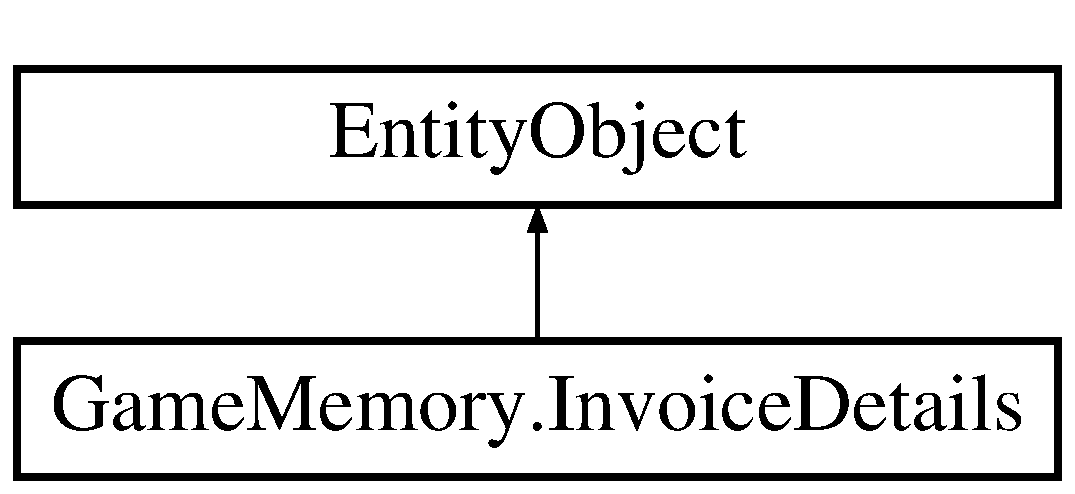
\includegraphics[height=2.000000cm]{class_game_memory_1_1_invoice_details}
\end{center}
\end{figure}
\subsection*{Static Public Member Functions}
\begin{DoxyCompactItemize}
\item 
static \hyperlink{class_game_memory_1_1_invoice_details}{Invoice\-Details} \hyperlink{class_game_memory_1_1_invoice_details_a857f5e20931749e50ad2892c99c4fd70}{Create\-Invoice\-Details} (global\-::\-System.\-Int32 invoice\-Details\-I\-D, global\-::\-System.\-Int32 invoice\-I\-D, global\-::\-System.\-String article, global\-::\-System.\-Int32 qty, global\-::\-System.\-Decimal price, global\-::\-System.\-Decimal v\-A\-T, global\-::\-System.\-Date\-Time time\-Stamp)
\begin{DoxyCompactList}\small\item\em Crear un nuevo objeto \hyperlink{class_game_memory_1_1_invoice_details}{Invoice\-Details}. \end{DoxyCompactList}\end{DoxyCompactItemize}
\subsection*{Properties}
\begin{DoxyCompactItemize}
\item 
global\-::\-System.\-Int32 \hyperlink{class_game_memory_1_1_invoice_details_aca50c426114254633fd034bc5a64854d}{Invoice\-Details\-I\-D}\hspace{0.3cm}{\ttfamily  \mbox{[}get, set\mbox{]}}
\begin{DoxyCompactList}\small\item\em No hay documentación de metadatos disponible. \end{DoxyCompactList}\item 
global\-::\-System.\-Int32 \hyperlink{class_game_memory_1_1_invoice_details_a67999662697ed10076327e47bba74611}{Invoice\-I\-D}\hspace{0.3cm}{\ttfamily  \mbox{[}get, set\mbox{]}}
\begin{DoxyCompactList}\small\item\em No hay documentación de metadatos disponible. \end{DoxyCompactList}\item 
global\-::\-System.\-String \hyperlink{class_game_memory_1_1_invoice_details_abc5eef71cea2b1720b5b0179ddf6fbf8}{Article}\hspace{0.3cm}{\ttfamily  \mbox{[}get, set\mbox{]}}
\begin{DoxyCompactList}\small\item\em No hay documentación de metadatos disponible. \end{DoxyCompactList}\item 
global\-::\-System.\-Int32 \hyperlink{class_game_memory_1_1_invoice_details_a8b4d80acf70dd427b45bb37590705813}{Qty}\hspace{0.3cm}{\ttfamily  \mbox{[}get, set\mbox{]}}
\begin{DoxyCompactList}\small\item\em No hay documentación de metadatos disponible. \end{DoxyCompactList}\item 
global\-::\-System.\-Decimal \hyperlink{class_game_memory_1_1_invoice_details_a4022db9ebe3d673e24f09290d966ff5e}{Price}\hspace{0.3cm}{\ttfamily  \mbox{[}get, set\mbox{]}}
\begin{DoxyCompactList}\small\item\em No hay documentación de metadatos disponible. \end{DoxyCompactList}\item 
global\-::\-System.\-Decimal \hyperlink{class_game_memory_1_1_invoice_details_a593bcc7bd0bcb2e41e6e531065413915}{V\-A\-T}\hspace{0.3cm}{\ttfamily  \mbox{[}get, set\mbox{]}}
\begin{DoxyCompactList}\small\item\em No hay documentación de metadatos disponible. \end{DoxyCompactList}\item 
global\-::\-System.\-Date\-Time \hyperlink{class_game_memory_1_1_invoice_details_aa68004d539f2d3f74d809cf395085d5c}{Time\-Stamp}\hspace{0.3cm}{\ttfamily  \mbox{[}get, set\mbox{]}}
\begin{DoxyCompactList}\small\item\em No hay documentación de metadatos disponible. \end{DoxyCompactList}\item 
\hyperlink{class_game_memory_1_1_invoices}{Invoices} \hyperlink{class_game_memory_1_1_invoice_details_a992833a86798d5b67073419b0106d7ec}{Invoices}\hspace{0.3cm}{\ttfamily  \mbox{[}get, set\mbox{]}}
\begin{DoxyCompactList}\small\item\em No hay documentación de metadatos disponible. \end{DoxyCompactList}\item 
Entity\-Reference$<$ \hyperlink{class_game_memory_1_1_invoices}{Invoices} $>$ \hyperlink{class_game_memory_1_1_invoice_details_addfc996d0bd6283ba9558d5f84a8c781}{Invoices\-Reference}\hspace{0.3cm}{\ttfamily  \mbox{[}get, set\mbox{]}}
\begin{DoxyCompactList}\small\item\em No hay documentación de metadatos disponible. \end{DoxyCompactList}\end{DoxyCompactItemize}


\subsection{Detailed Description}
No hay documentación de metadatos disponible. 



\subsection{Member Function Documentation}
\hypertarget{class_game_memory_1_1_invoice_details_a857f5e20931749e50ad2892c99c4fd70}{\index{Game\-Memory\-::\-Invoice\-Details@{Game\-Memory\-::\-Invoice\-Details}!Create\-Invoice\-Details@{Create\-Invoice\-Details}}
\index{Create\-Invoice\-Details@{Create\-Invoice\-Details}!GameMemory::InvoiceDetails@{Game\-Memory\-::\-Invoice\-Details}}
\subsubsection[{Create\-Invoice\-Details}]{\setlength{\rightskip}{0pt plus 5cm}static {\bf Invoice\-Details} Game\-Memory.\-Invoice\-Details.\-Create\-Invoice\-Details (
\begin{DoxyParamCaption}
\item[{global\-::\-System.\-Int32}]{invoice\-Details\-I\-D, }
\item[{global\-::\-System.\-Int32}]{invoice\-I\-D, }
\item[{global\-::\-System.\-String}]{article, }
\item[{global\-::\-System.\-Int32}]{qty, }
\item[{global\-::\-System.\-Decimal}]{price, }
\item[{global\-::\-System.\-Decimal}]{v\-A\-T, }
\item[{global\-::\-System.\-Date\-Time}]{time\-Stamp}
\end{DoxyParamCaption}
)\hspace{0.3cm}{\ttfamily [static]}}}\label{class_game_memory_1_1_invoice_details_a857f5e20931749e50ad2892c99c4fd70}


Crear un nuevo objeto \hyperlink{class_game_memory_1_1_invoice_details}{Invoice\-Details}. 


\begin{DoxyParams}{Parameters}
{\em invoice\-Details\-I\-D} & Valor inicial de la propiedad Invoice\-Details\-I\-D.\\
\hline
{\em invoice\-I\-D} & Valor inicial de la propiedad Invoice\-I\-D.\\
\hline
{\em article} & Valor inicial de la propiedad Article.\\
\hline
{\em qty} & Valor inicial de la propiedad Qty.\\
\hline
{\em price} & Valor inicial de la propiedad Price.\\
\hline
{\em v\-A\-T} & Valor inicial de la propiedad V\-A\-T.\\
\hline
{\em time\-Stamp} & Valor inicial de la propiedad Time\-Stamp.\\
\hline
\end{DoxyParams}


\subsection{Property Documentation}
\hypertarget{class_game_memory_1_1_invoice_details_abc5eef71cea2b1720b5b0179ddf6fbf8}{\index{Game\-Memory\-::\-Invoice\-Details@{Game\-Memory\-::\-Invoice\-Details}!Article@{Article}}
\index{Article@{Article}!GameMemory::InvoiceDetails@{Game\-Memory\-::\-Invoice\-Details}}
\subsubsection[{Article}]{\setlength{\rightskip}{0pt plus 5cm}global.\-System.\-String Game\-Memory.\-Invoice\-Details.\-Article\hspace{0.3cm}{\ttfamily [get]}, {\ttfamily [set]}}}\label{class_game_memory_1_1_invoice_details_abc5eef71cea2b1720b5b0179ddf6fbf8}


No hay documentación de metadatos disponible. 

\hypertarget{class_game_memory_1_1_invoice_details_aca50c426114254633fd034bc5a64854d}{\index{Game\-Memory\-::\-Invoice\-Details@{Game\-Memory\-::\-Invoice\-Details}!Invoice\-Details\-I\-D@{Invoice\-Details\-I\-D}}
\index{Invoice\-Details\-I\-D@{Invoice\-Details\-I\-D}!GameMemory::InvoiceDetails@{Game\-Memory\-::\-Invoice\-Details}}
\subsubsection[{Invoice\-Details\-I\-D}]{\setlength{\rightskip}{0pt plus 5cm}global.\-System.\-Int32 Game\-Memory.\-Invoice\-Details.\-Invoice\-Details\-I\-D\hspace{0.3cm}{\ttfamily [get]}, {\ttfamily [set]}}}\label{class_game_memory_1_1_invoice_details_aca50c426114254633fd034bc5a64854d}


No hay documentación de metadatos disponible. 

\hypertarget{class_game_memory_1_1_invoice_details_a67999662697ed10076327e47bba74611}{\index{Game\-Memory\-::\-Invoice\-Details@{Game\-Memory\-::\-Invoice\-Details}!Invoice\-I\-D@{Invoice\-I\-D}}
\index{Invoice\-I\-D@{Invoice\-I\-D}!GameMemory::InvoiceDetails@{Game\-Memory\-::\-Invoice\-Details}}
\subsubsection[{Invoice\-I\-D}]{\setlength{\rightskip}{0pt plus 5cm}global.\-System.\-Int32 Game\-Memory.\-Invoice\-Details.\-Invoice\-I\-D\hspace{0.3cm}{\ttfamily [get]}, {\ttfamily [set]}}}\label{class_game_memory_1_1_invoice_details_a67999662697ed10076327e47bba74611}


No hay documentación de metadatos disponible. 

\hypertarget{class_game_memory_1_1_invoice_details_a992833a86798d5b67073419b0106d7ec}{\index{Game\-Memory\-::\-Invoice\-Details@{Game\-Memory\-::\-Invoice\-Details}!Invoices@{Invoices}}
\index{Invoices@{Invoices}!GameMemory::InvoiceDetails@{Game\-Memory\-::\-Invoice\-Details}}
\subsubsection[{Invoices}]{\setlength{\rightskip}{0pt plus 5cm}{\bf Invoices} Game\-Memory.\-Invoice\-Details.\-Invoices\hspace{0.3cm}{\ttfamily [get]}, {\ttfamily [set]}}}\label{class_game_memory_1_1_invoice_details_a992833a86798d5b67073419b0106d7ec}


No hay documentación de metadatos disponible. 

\hypertarget{class_game_memory_1_1_invoice_details_addfc996d0bd6283ba9558d5f84a8c781}{\index{Game\-Memory\-::\-Invoice\-Details@{Game\-Memory\-::\-Invoice\-Details}!Invoices\-Reference@{Invoices\-Reference}}
\index{Invoices\-Reference@{Invoices\-Reference}!GameMemory::InvoiceDetails@{Game\-Memory\-::\-Invoice\-Details}}
\subsubsection[{Invoices\-Reference}]{\setlength{\rightskip}{0pt plus 5cm}Entity\-Reference$<${\bf Invoices}$>$ Game\-Memory.\-Invoice\-Details.\-Invoices\-Reference\hspace{0.3cm}{\ttfamily [get]}, {\ttfamily [set]}}}\label{class_game_memory_1_1_invoice_details_addfc996d0bd6283ba9558d5f84a8c781}


No hay documentación de metadatos disponible. 

\hypertarget{class_game_memory_1_1_invoice_details_a4022db9ebe3d673e24f09290d966ff5e}{\index{Game\-Memory\-::\-Invoice\-Details@{Game\-Memory\-::\-Invoice\-Details}!Price@{Price}}
\index{Price@{Price}!GameMemory::InvoiceDetails@{Game\-Memory\-::\-Invoice\-Details}}
\subsubsection[{Price}]{\setlength{\rightskip}{0pt plus 5cm}global.\-System.\-Decimal Game\-Memory.\-Invoice\-Details.\-Price\hspace{0.3cm}{\ttfamily [get]}, {\ttfamily [set]}}}\label{class_game_memory_1_1_invoice_details_a4022db9ebe3d673e24f09290d966ff5e}


No hay documentación de metadatos disponible. 

\hypertarget{class_game_memory_1_1_invoice_details_a8b4d80acf70dd427b45bb37590705813}{\index{Game\-Memory\-::\-Invoice\-Details@{Game\-Memory\-::\-Invoice\-Details}!Qty@{Qty}}
\index{Qty@{Qty}!GameMemory::InvoiceDetails@{Game\-Memory\-::\-Invoice\-Details}}
\subsubsection[{Qty}]{\setlength{\rightskip}{0pt plus 5cm}global.\-System.\-Int32 Game\-Memory.\-Invoice\-Details.\-Qty\hspace{0.3cm}{\ttfamily [get]}, {\ttfamily [set]}}}\label{class_game_memory_1_1_invoice_details_a8b4d80acf70dd427b45bb37590705813}


No hay documentación de metadatos disponible. 

\hypertarget{class_game_memory_1_1_invoice_details_aa68004d539f2d3f74d809cf395085d5c}{\index{Game\-Memory\-::\-Invoice\-Details@{Game\-Memory\-::\-Invoice\-Details}!Time\-Stamp@{Time\-Stamp}}
\index{Time\-Stamp@{Time\-Stamp}!GameMemory::InvoiceDetails@{Game\-Memory\-::\-Invoice\-Details}}
\subsubsection[{Time\-Stamp}]{\setlength{\rightskip}{0pt plus 5cm}global.\-System.\-Date\-Time Game\-Memory.\-Invoice\-Details.\-Time\-Stamp\hspace{0.3cm}{\ttfamily [get]}, {\ttfamily [set]}}}\label{class_game_memory_1_1_invoice_details_aa68004d539f2d3f74d809cf395085d5c}


No hay documentación de metadatos disponible. 

\hypertarget{class_game_memory_1_1_invoice_details_a593bcc7bd0bcb2e41e6e531065413915}{\index{Game\-Memory\-::\-Invoice\-Details@{Game\-Memory\-::\-Invoice\-Details}!V\-A\-T@{V\-A\-T}}
\index{V\-A\-T@{V\-A\-T}!GameMemory::InvoiceDetails@{Game\-Memory\-::\-Invoice\-Details}}
\subsubsection[{V\-A\-T}]{\setlength{\rightskip}{0pt plus 5cm}global.\-System.\-Decimal Game\-Memory.\-Invoice\-Details.\-V\-A\-T\hspace{0.3cm}{\ttfamily [get]}, {\ttfamily [set]}}}\label{class_game_memory_1_1_invoice_details_a593bcc7bd0bcb2e41e6e531065413915}


No hay documentación de metadatos disponible. 



The documentation for this class was generated from the following file\-:\begin{DoxyCompactItemize}
\item 
D\-:/tesis\-Assembla/branches/\-Branch\-\_\-\-Tesis\-\_\-\-Sprint01/\-Dev/\-Interaction Module/\-Game\-Memory/\-Game\-Memory/O\-M\-K\-T.\-Designer.\-cs\end{DoxyCompactItemize}

\hypertarget{class_game_memory_1_1_invoices}{\section{Game\-Memory.\-Invoices Class Reference}
\label{class_game_memory_1_1_invoices}\index{Game\-Memory.\-Invoices@{Game\-Memory.\-Invoices}}
}


No hay documentación de metadatos disponible.  


Inheritance diagram for Game\-Memory.\-Invoices\-:\begin{figure}[H]
\begin{center}
\leavevmode
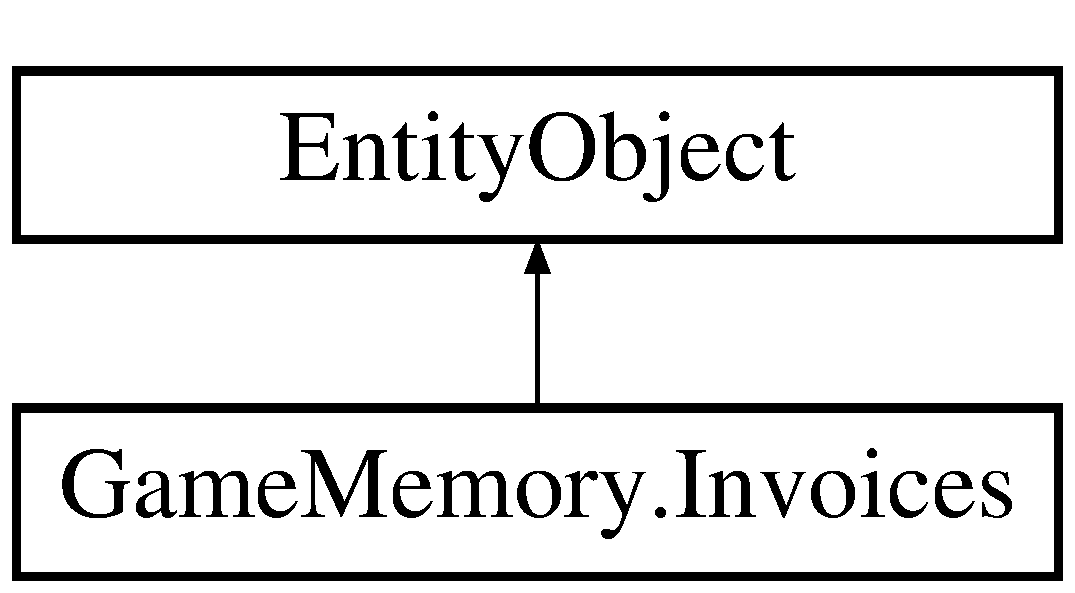
\includegraphics[height=2.000000cm]{class_game_memory_1_1_invoices}
\end{center}
\end{figure}
\subsection*{Static Public Member Functions}
\begin{DoxyCompactItemize}
\item 
static \hyperlink{class_game_memory_1_1_invoices}{Invoices} \hyperlink{class_game_memory_1_1_invoices_a386fad50c526991afab04b32057e18fe}{Create\-Invoices} (global\-::\-System.\-Int32 invoice\-I\-D, global\-::\-System.\-Int32 invoice\-Number, global\-::\-System.\-Int32 customer\-I\-D, global\-::\-System.\-String notes, global\-::\-System.\-Date\-Time time\-Stamp, global\-::\-System.\-Date\-Time due\-Date, global\-::\-System.\-Decimal advance\-Payment\-Tax, global\-::\-System.\-Boolean paid)
\begin{DoxyCompactList}\small\item\em Crear un nuevo objeto \hyperlink{class_game_memory_1_1_invoices}{Invoices}. \end{DoxyCompactList}\end{DoxyCompactItemize}
\subsection*{Properties}
\begin{DoxyCompactItemize}
\item 
global\-::\-System.\-Int32 \hyperlink{class_game_memory_1_1_invoices_a5e354613497aec5c10ef302d9d9e7258}{Invoice\-I\-D}\hspace{0.3cm}{\ttfamily  \mbox{[}get, set\mbox{]}}
\begin{DoxyCompactList}\small\item\em No hay documentación de metadatos disponible. \end{DoxyCompactList}\item 
global\-::\-System.\-Int32 \hyperlink{class_game_memory_1_1_invoices_ae1338eba0dcd9ebfc1ae59ee289c9c15}{Invoice\-Number}\hspace{0.3cm}{\ttfamily  \mbox{[}get, set\mbox{]}}
\begin{DoxyCompactList}\small\item\em No hay documentación de metadatos disponible. \end{DoxyCompactList}\item 
global\-::\-System.\-Int32 \hyperlink{class_game_memory_1_1_invoices_aae5190344c921ece5f25d62d34200c33}{Customer\-I\-D}\hspace{0.3cm}{\ttfamily  \mbox{[}get, set\mbox{]}}
\begin{DoxyCompactList}\small\item\em No hay documentación de metadatos disponible. \end{DoxyCompactList}\item 
global\-::\-System.\-String \hyperlink{class_game_memory_1_1_invoices_a82fa8e4d468479126d9f05e6590bd95f}{Name}\hspace{0.3cm}{\ttfamily  \mbox{[}get, set\mbox{]}}
\begin{DoxyCompactList}\small\item\em No hay documentación de metadatos disponible. \end{DoxyCompactList}\item 
global\-::\-System.\-String \hyperlink{class_game_memory_1_1_invoices_a5e477e04fbcd9ad7185e8262af528be3}{Notes}\hspace{0.3cm}{\ttfamily  \mbox{[}get, set\mbox{]}}
\begin{DoxyCompactList}\small\item\em No hay documentación de metadatos disponible. \end{DoxyCompactList}\item 
global\-::\-System.\-String \hyperlink{class_game_memory_1_1_invoices_a381a2b51810c12b0c4c5e7603c0ae942}{Proposal\-Details}\hspace{0.3cm}{\ttfamily  \mbox{[}get, set\mbox{]}}
\begin{DoxyCompactList}\small\item\em No hay documentación de metadatos disponible. \end{DoxyCompactList}\item 
global\-::\-System.\-Date\-Time \hyperlink{class_game_memory_1_1_invoices_af2fd7641a9681d57e3aa2583bc90b458}{Time\-Stamp}\hspace{0.3cm}{\ttfamily  \mbox{[}get, set\mbox{]}}
\begin{DoxyCompactList}\small\item\em No hay documentación de metadatos disponible. \end{DoxyCompactList}\item 
global\-::\-System.\-Date\-Time \hyperlink{class_game_memory_1_1_invoices_a34f6ae1c319669d255f64b19e6574218}{Due\-Date}\hspace{0.3cm}{\ttfamily  \mbox{[}get, set\mbox{]}}
\begin{DoxyCompactList}\small\item\em No hay documentación de metadatos disponible. \end{DoxyCompactList}\item 
global\-::\-System.\-Decimal \hyperlink{class_game_memory_1_1_invoices_a4c8fb4bba4408487adde6b055abec055}{Advance\-Payment\-Tax}\hspace{0.3cm}{\ttfamily  \mbox{[}get, set\mbox{]}}
\begin{DoxyCompactList}\small\item\em No hay documentación de metadatos disponible. \end{DoxyCompactList}\item 
global\-::\-System.\-Boolean \hyperlink{class_game_memory_1_1_invoices_a494ac26836e51198ef21d28dbe0c63e4}{Paid}\hspace{0.3cm}{\ttfamily  \mbox{[}get, set\mbox{]}}
\begin{DoxyCompactList}\small\item\em No hay documentación de metadatos disponible. \end{DoxyCompactList}\item 
\hyperlink{class_game_memory_1_1_customers}{Customers} \hyperlink{class_game_memory_1_1_invoices_a0acb5cf5f80c7dcda908489338671b37}{Customers}\hspace{0.3cm}{\ttfamily  \mbox{[}get, set\mbox{]}}
\begin{DoxyCompactList}\small\item\em No hay documentación de metadatos disponible. \end{DoxyCompactList}\item 
Entity\-Reference$<$ \hyperlink{class_game_memory_1_1_customers}{Customers} $>$ \hyperlink{class_game_memory_1_1_invoices_af845c24d8cd3d0bad861299e693e5b0e}{Customers\-Reference}\hspace{0.3cm}{\ttfamily  \mbox{[}get, set\mbox{]}}
\begin{DoxyCompactList}\small\item\em No hay documentación de metadatos disponible. \end{DoxyCompactList}\item 
Entity\-Collection$<$ \hyperlink{class_game_memory_1_1_invoice_details}{Invoice\-Details} $>$ \hyperlink{class_game_memory_1_1_invoices_a5ae6f975426aa0a9f86af85e03e23f10}{Invoice\-Details}\hspace{0.3cm}{\ttfamily  \mbox{[}get, set\mbox{]}}
\begin{DoxyCompactList}\small\item\em No hay documentación de metadatos disponible. \end{DoxyCompactList}\end{DoxyCompactItemize}


\subsection{Detailed Description}
No hay documentación de metadatos disponible. 



\subsection{Member Function Documentation}
\hypertarget{class_game_memory_1_1_invoices_a386fad50c526991afab04b32057e18fe}{\index{Game\-Memory\-::\-Invoices@{Game\-Memory\-::\-Invoices}!Create\-Invoices@{Create\-Invoices}}
\index{Create\-Invoices@{Create\-Invoices}!GameMemory::Invoices@{Game\-Memory\-::\-Invoices}}
\subsubsection[{Create\-Invoices}]{\setlength{\rightskip}{0pt plus 5cm}static {\bf Invoices} Game\-Memory.\-Invoices.\-Create\-Invoices (
\begin{DoxyParamCaption}
\item[{global\-::\-System.\-Int32}]{invoice\-I\-D, }
\item[{global\-::\-System.\-Int32}]{invoice\-Number, }
\item[{global\-::\-System.\-Int32}]{customer\-I\-D, }
\item[{global\-::\-System.\-String}]{notes, }
\item[{global\-::\-System.\-Date\-Time}]{time\-Stamp, }
\item[{global\-::\-System.\-Date\-Time}]{due\-Date, }
\item[{global\-::\-System.\-Decimal}]{advance\-Payment\-Tax, }
\item[{global\-::\-System.\-Boolean}]{paid}
\end{DoxyParamCaption}
)\hspace{0.3cm}{\ttfamily [static]}}}\label{class_game_memory_1_1_invoices_a386fad50c526991afab04b32057e18fe}


Crear un nuevo objeto \hyperlink{class_game_memory_1_1_invoices}{Invoices}. 


\begin{DoxyParams}{Parameters}
{\em invoice\-I\-D} & Valor inicial de la propiedad Invoice\-I\-D.\\
\hline
{\em invoice\-Number} & Valor inicial de la propiedad Invoice\-Number.\\
\hline
{\em customer\-I\-D} & Valor inicial de la propiedad Customer\-I\-D.\\
\hline
{\em notes} & Valor inicial de la propiedad Notes.\\
\hline
{\em time\-Stamp} & Valor inicial de la propiedad Time\-Stamp.\\
\hline
{\em due\-Date} & Valor inicial de la propiedad Due\-Date.\\
\hline
{\em advance\-Payment\-Tax} & Valor inicial de la propiedad Advance\-Payment\-Tax.\\
\hline
{\em paid} & Valor inicial de la propiedad Paid.\\
\hline
\end{DoxyParams}


\subsection{Property Documentation}
\hypertarget{class_game_memory_1_1_invoices_a4c8fb4bba4408487adde6b055abec055}{\index{Game\-Memory\-::\-Invoices@{Game\-Memory\-::\-Invoices}!Advance\-Payment\-Tax@{Advance\-Payment\-Tax}}
\index{Advance\-Payment\-Tax@{Advance\-Payment\-Tax}!GameMemory::Invoices@{Game\-Memory\-::\-Invoices}}
\subsubsection[{Advance\-Payment\-Tax}]{\setlength{\rightskip}{0pt plus 5cm}global.\-System.\-Decimal Game\-Memory.\-Invoices.\-Advance\-Payment\-Tax\hspace{0.3cm}{\ttfamily [get]}, {\ttfamily [set]}}}\label{class_game_memory_1_1_invoices_a4c8fb4bba4408487adde6b055abec055}


No hay documentación de metadatos disponible. 

\hypertarget{class_game_memory_1_1_invoices_aae5190344c921ece5f25d62d34200c33}{\index{Game\-Memory\-::\-Invoices@{Game\-Memory\-::\-Invoices}!Customer\-I\-D@{Customer\-I\-D}}
\index{Customer\-I\-D@{Customer\-I\-D}!GameMemory::Invoices@{Game\-Memory\-::\-Invoices}}
\subsubsection[{Customer\-I\-D}]{\setlength{\rightskip}{0pt plus 5cm}global.\-System.\-Int32 Game\-Memory.\-Invoices.\-Customer\-I\-D\hspace{0.3cm}{\ttfamily [get]}, {\ttfamily [set]}}}\label{class_game_memory_1_1_invoices_aae5190344c921ece5f25d62d34200c33}


No hay documentación de metadatos disponible. 

\hypertarget{class_game_memory_1_1_invoices_a0acb5cf5f80c7dcda908489338671b37}{\index{Game\-Memory\-::\-Invoices@{Game\-Memory\-::\-Invoices}!Customers@{Customers}}
\index{Customers@{Customers}!GameMemory::Invoices@{Game\-Memory\-::\-Invoices}}
\subsubsection[{Customers}]{\setlength{\rightskip}{0pt plus 5cm}{\bf Customers} Game\-Memory.\-Invoices.\-Customers\hspace{0.3cm}{\ttfamily [get]}, {\ttfamily [set]}}}\label{class_game_memory_1_1_invoices_a0acb5cf5f80c7dcda908489338671b37}


No hay documentación de metadatos disponible. 

\hypertarget{class_game_memory_1_1_invoices_af845c24d8cd3d0bad861299e693e5b0e}{\index{Game\-Memory\-::\-Invoices@{Game\-Memory\-::\-Invoices}!Customers\-Reference@{Customers\-Reference}}
\index{Customers\-Reference@{Customers\-Reference}!GameMemory::Invoices@{Game\-Memory\-::\-Invoices}}
\subsubsection[{Customers\-Reference}]{\setlength{\rightskip}{0pt plus 5cm}Entity\-Reference$<${\bf Customers}$>$ Game\-Memory.\-Invoices.\-Customers\-Reference\hspace{0.3cm}{\ttfamily [get]}, {\ttfamily [set]}}}\label{class_game_memory_1_1_invoices_af845c24d8cd3d0bad861299e693e5b0e}


No hay documentación de metadatos disponible. 

\hypertarget{class_game_memory_1_1_invoices_a34f6ae1c319669d255f64b19e6574218}{\index{Game\-Memory\-::\-Invoices@{Game\-Memory\-::\-Invoices}!Due\-Date@{Due\-Date}}
\index{Due\-Date@{Due\-Date}!GameMemory::Invoices@{Game\-Memory\-::\-Invoices}}
\subsubsection[{Due\-Date}]{\setlength{\rightskip}{0pt plus 5cm}global.\-System.\-Date\-Time Game\-Memory.\-Invoices.\-Due\-Date\hspace{0.3cm}{\ttfamily [get]}, {\ttfamily [set]}}}\label{class_game_memory_1_1_invoices_a34f6ae1c319669d255f64b19e6574218}


No hay documentación de metadatos disponible. 

\hypertarget{class_game_memory_1_1_invoices_a5ae6f975426aa0a9f86af85e03e23f10}{\index{Game\-Memory\-::\-Invoices@{Game\-Memory\-::\-Invoices}!Invoice\-Details@{Invoice\-Details}}
\index{Invoice\-Details@{Invoice\-Details}!GameMemory::Invoices@{Game\-Memory\-::\-Invoices}}
\subsubsection[{Invoice\-Details}]{\setlength{\rightskip}{0pt plus 5cm}Entity\-Collection$<${\bf Invoice\-Details}$>$ Game\-Memory.\-Invoices.\-Invoice\-Details\hspace{0.3cm}{\ttfamily [get]}, {\ttfamily [set]}}}\label{class_game_memory_1_1_invoices_a5ae6f975426aa0a9f86af85e03e23f10}


No hay documentación de metadatos disponible. 

\hypertarget{class_game_memory_1_1_invoices_a5e354613497aec5c10ef302d9d9e7258}{\index{Game\-Memory\-::\-Invoices@{Game\-Memory\-::\-Invoices}!Invoice\-I\-D@{Invoice\-I\-D}}
\index{Invoice\-I\-D@{Invoice\-I\-D}!GameMemory::Invoices@{Game\-Memory\-::\-Invoices}}
\subsubsection[{Invoice\-I\-D}]{\setlength{\rightskip}{0pt plus 5cm}global.\-System.\-Int32 Game\-Memory.\-Invoices.\-Invoice\-I\-D\hspace{0.3cm}{\ttfamily [get]}, {\ttfamily [set]}}}\label{class_game_memory_1_1_invoices_a5e354613497aec5c10ef302d9d9e7258}


No hay documentación de metadatos disponible. 

\hypertarget{class_game_memory_1_1_invoices_ae1338eba0dcd9ebfc1ae59ee289c9c15}{\index{Game\-Memory\-::\-Invoices@{Game\-Memory\-::\-Invoices}!Invoice\-Number@{Invoice\-Number}}
\index{Invoice\-Number@{Invoice\-Number}!GameMemory::Invoices@{Game\-Memory\-::\-Invoices}}
\subsubsection[{Invoice\-Number}]{\setlength{\rightskip}{0pt plus 5cm}global.\-System.\-Int32 Game\-Memory.\-Invoices.\-Invoice\-Number\hspace{0.3cm}{\ttfamily [get]}, {\ttfamily [set]}}}\label{class_game_memory_1_1_invoices_ae1338eba0dcd9ebfc1ae59ee289c9c15}


No hay documentación de metadatos disponible. 

\hypertarget{class_game_memory_1_1_invoices_a82fa8e4d468479126d9f05e6590bd95f}{\index{Game\-Memory\-::\-Invoices@{Game\-Memory\-::\-Invoices}!Name@{Name}}
\index{Name@{Name}!GameMemory::Invoices@{Game\-Memory\-::\-Invoices}}
\subsubsection[{Name}]{\setlength{\rightskip}{0pt plus 5cm}global.\-System.\-String Game\-Memory.\-Invoices.\-Name\hspace{0.3cm}{\ttfamily [get]}, {\ttfamily [set]}}}\label{class_game_memory_1_1_invoices_a82fa8e4d468479126d9f05e6590bd95f}


No hay documentación de metadatos disponible. 

\hypertarget{class_game_memory_1_1_invoices_a5e477e04fbcd9ad7185e8262af528be3}{\index{Game\-Memory\-::\-Invoices@{Game\-Memory\-::\-Invoices}!Notes@{Notes}}
\index{Notes@{Notes}!GameMemory::Invoices@{Game\-Memory\-::\-Invoices}}
\subsubsection[{Notes}]{\setlength{\rightskip}{0pt plus 5cm}global.\-System.\-String Game\-Memory.\-Invoices.\-Notes\hspace{0.3cm}{\ttfamily [get]}, {\ttfamily [set]}}}\label{class_game_memory_1_1_invoices_a5e477e04fbcd9ad7185e8262af528be3}


No hay documentación de metadatos disponible. 

\hypertarget{class_game_memory_1_1_invoices_a494ac26836e51198ef21d28dbe0c63e4}{\index{Game\-Memory\-::\-Invoices@{Game\-Memory\-::\-Invoices}!Paid@{Paid}}
\index{Paid@{Paid}!GameMemory::Invoices@{Game\-Memory\-::\-Invoices}}
\subsubsection[{Paid}]{\setlength{\rightskip}{0pt plus 5cm}global.\-System.\-Boolean Game\-Memory.\-Invoices.\-Paid\hspace{0.3cm}{\ttfamily [get]}, {\ttfamily [set]}}}\label{class_game_memory_1_1_invoices_a494ac26836e51198ef21d28dbe0c63e4}


No hay documentación de metadatos disponible. 

\hypertarget{class_game_memory_1_1_invoices_a381a2b51810c12b0c4c5e7603c0ae942}{\index{Game\-Memory\-::\-Invoices@{Game\-Memory\-::\-Invoices}!Proposal\-Details@{Proposal\-Details}}
\index{Proposal\-Details@{Proposal\-Details}!GameMemory::Invoices@{Game\-Memory\-::\-Invoices}}
\subsubsection[{Proposal\-Details}]{\setlength{\rightskip}{0pt plus 5cm}global.\-System.\-String Game\-Memory.\-Invoices.\-Proposal\-Details\hspace{0.3cm}{\ttfamily [get]}, {\ttfamily [set]}}}\label{class_game_memory_1_1_invoices_a381a2b51810c12b0c4c5e7603c0ae942}


No hay documentación de metadatos disponible. 

\hypertarget{class_game_memory_1_1_invoices_af2fd7641a9681d57e3aa2583bc90b458}{\index{Game\-Memory\-::\-Invoices@{Game\-Memory\-::\-Invoices}!Time\-Stamp@{Time\-Stamp}}
\index{Time\-Stamp@{Time\-Stamp}!GameMemory::Invoices@{Game\-Memory\-::\-Invoices}}
\subsubsection[{Time\-Stamp}]{\setlength{\rightskip}{0pt plus 5cm}global.\-System.\-Date\-Time Game\-Memory.\-Invoices.\-Time\-Stamp\hspace{0.3cm}{\ttfamily [get]}, {\ttfamily [set]}}}\label{class_game_memory_1_1_invoices_af2fd7641a9681d57e3aa2583bc90b458}


No hay documentación de metadatos disponible. 



The documentation for this class was generated from the following file\-:\begin{DoxyCompactItemize}
\item 
D\-:/tesis\-Assembla/branches/\-Branch\-\_\-\-Tesis\-\_\-\-Sprint01/\-Dev/\-Interaction Module/\-Game\-Memory/\-Game\-Memory/O\-M\-K\-T.\-Designer.\-cs\end{DoxyCompactItemize}

\hypertarget{class_game_memory_1_1_locations}{\section{Game\-Memory.\-Locations Class Reference}
\label{class_game_memory_1_1_locations}\index{Game\-Memory.\-Locations@{Game\-Memory.\-Locations}}
}


No hay documentación de metadatos disponible.  


Inheritance diagram for Game\-Memory.\-Locations\-:\begin{figure}[H]
\begin{center}
\leavevmode
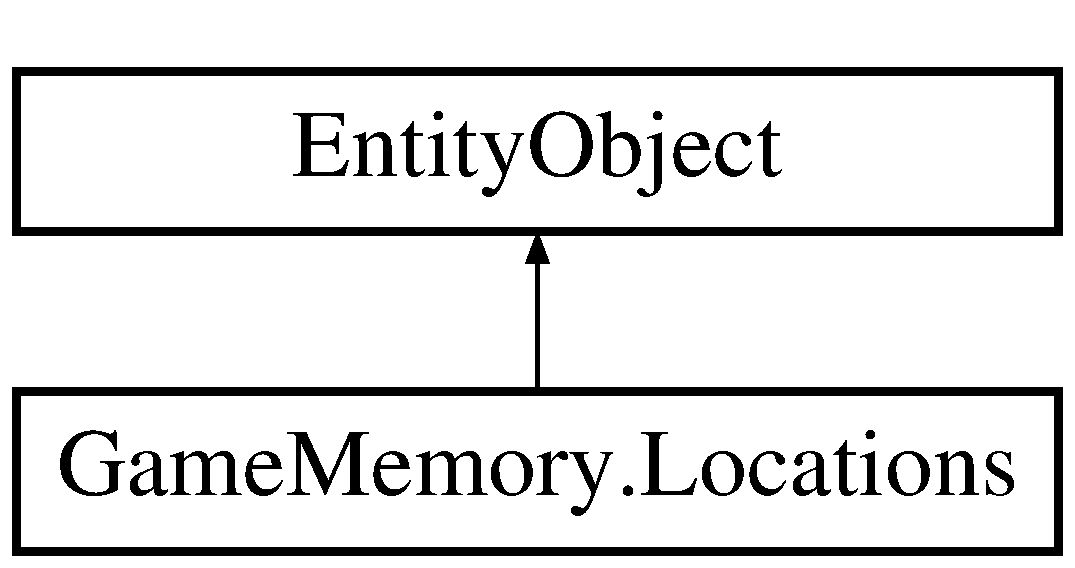
\includegraphics[height=2.000000cm]{class_game_memory_1_1_locations}
\end{center}
\end{figure}
\subsection*{Static Public Member Functions}
\begin{DoxyCompactItemize}
\item 
static \hyperlink{class_game_memory_1_1_locations}{Locations} \hyperlink{class_game_memory_1_1_locations_a473576211dcf70178087393084d262e1}{Create\-Locations} (global\-::\-System.\-Int32 location\-Id, global\-::\-System.\-Int32 reference\-Number)
\begin{DoxyCompactList}\small\item\em Crear un nuevo objeto \hyperlink{class_game_memory_1_1_locations}{Locations}. \end{DoxyCompactList}\end{DoxyCompactItemize}
\subsection*{Properties}
\begin{DoxyCompactItemize}
\item 
global\-::\-System.\-Int32 \hyperlink{class_game_memory_1_1_locations_a701a32d74857333fff435f05e2ce9f6a}{Location\-Id}\hspace{0.3cm}{\ttfamily  \mbox{[}get, set\mbox{]}}
\begin{DoxyCompactList}\small\item\em No hay documentación de metadatos disponible. \end{DoxyCompactList}\item 
global\-::\-System.\-String \hyperlink{class_game_memory_1_1_locations_a9bfc421c1b405e1abc46caa06a9f32df}{Latitude}\hspace{0.3cm}{\ttfamily  \mbox{[}get, set\mbox{]}}
\begin{DoxyCompactList}\small\item\em No hay documentación de metadatos disponible. \end{DoxyCompactList}\item 
global\-::\-System.\-String \hyperlink{class_game_memory_1_1_locations_a1e157ff8446d76da3fff6479e73d910c}{Longitude}\hspace{0.3cm}{\ttfamily  \mbox{[}get, set\mbox{]}}
\begin{DoxyCompactList}\small\item\em No hay documentación de metadatos disponible. \end{DoxyCompactList}\item 
global\-::\-System.\-String \hyperlink{class_game_memory_1_1_locations_a6c2715b80d375ead97d530deb4f20f87}{Detail}\hspace{0.3cm}{\ttfamily  \mbox{[}get, set\mbox{]}}
\begin{DoxyCompactList}\small\item\em No hay documentación de metadatos disponible. \end{DoxyCompactList}\item 
global\-::\-System.\-String \hyperlink{class_game_memory_1_1_locations_a03b9430eb5232aa3555f117bc4b2bdca}{Adress}\hspace{0.3cm}{\ttfamily  \mbox{[}get, set\mbox{]}}
\begin{DoxyCompactList}\small\item\em No hay documentación de metadatos disponible. \end{DoxyCompactList}\item 
global\-::\-System.\-Int32 \hyperlink{class_game_memory_1_1_locations_ab0156c8a60262ce8d1665214335fd7aa}{Reference\-Number}\hspace{0.3cm}{\ttfamily  \mbox{[}get, set\mbox{]}}
\begin{DoxyCompactList}\small\item\em No hay documentación de metadatos disponible. \end{DoxyCompactList}\item 
Entity\-Collection$<$ \hyperlink{class_game_memory_1_1_advert_hosts}{Advert\-Hosts} $>$ \hyperlink{class_game_memory_1_1_locations_a34dae26338430d0e0f1e394dcd06c502}{Advert\-Hosts}\hspace{0.3cm}{\ttfamily  \mbox{[}get, set\mbox{]}}
\begin{DoxyCompactList}\small\item\em No hay documentación de metadatos disponible. \end{DoxyCompactList}\end{DoxyCompactItemize}


\subsection{Detailed Description}
No hay documentación de metadatos disponible. 



\subsection{Member Function Documentation}
\hypertarget{class_game_memory_1_1_locations_a473576211dcf70178087393084d262e1}{\index{Game\-Memory\-::\-Locations@{Game\-Memory\-::\-Locations}!Create\-Locations@{Create\-Locations}}
\index{Create\-Locations@{Create\-Locations}!GameMemory::Locations@{Game\-Memory\-::\-Locations}}
\subsubsection[{Create\-Locations}]{\setlength{\rightskip}{0pt plus 5cm}static {\bf Locations} Game\-Memory.\-Locations.\-Create\-Locations (
\begin{DoxyParamCaption}
\item[{global\-::\-System.\-Int32}]{location\-Id, }
\item[{global\-::\-System.\-Int32}]{reference\-Number}
\end{DoxyParamCaption}
)\hspace{0.3cm}{\ttfamily [static]}}}\label{class_game_memory_1_1_locations_a473576211dcf70178087393084d262e1}


Crear un nuevo objeto \hyperlink{class_game_memory_1_1_locations}{Locations}. 


\begin{DoxyParams}{Parameters}
{\em location\-Id} & Valor inicial de la propiedad Location\-Id.\\
\hline
{\em reference\-Number} & Valor inicial de la propiedad Reference\-Number.\\
\hline
\end{DoxyParams}


\subsection{Property Documentation}
\hypertarget{class_game_memory_1_1_locations_a03b9430eb5232aa3555f117bc4b2bdca}{\index{Game\-Memory\-::\-Locations@{Game\-Memory\-::\-Locations}!Adress@{Adress}}
\index{Adress@{Adress}!GameMemory::Locations@{Game\-Memory\-::\-Locations}}
\subsubsection[{Adress}]{\setlength{\rightskip}{0pt plus 5cm}global.\-System.\-String Game\-Memory.\-Locations.\-Adress\hspace{0.3cm}{\ttfamily [get]}, {\ttfamily [set]}}}\label{class_game_memory_1_1_locations_a03b9430eb5232aa3555f117bc4b2bdca}


No hay documentación de metadatos disponible. 

\hypertarget{class_game_memory_1_1_locations_a34dae26338430d0e0f1e394dcd06c502}{\index{Game\-Memory\-::\-Locations@{Game\-Memory\-::\-Locations}!Advert\-Hosts@{Advert\-Hosts}}
\index{Advert\-Hosts@{Advert\-Hosts}!GameMemory::Locations@{Game\-Memory\-::\-Locations}}
\subsubsection[{Advert\-Hosts}]{\setlength{\rightskip}{0pt plus 5cm}Entity\-Collection$<${\bf Advert\-Hosts}$>$ Game\-Memory.\-Locations.\-Advert\-Hosts\hspace{0.3cm}{\ttfamily [get]}, {\ttfamily [set]}}}\label{class_game_memory_1_1_locations_a34dae26338430d0e0f1e394dcd06c502}


No hay documentación de metadatos disponible. 

\hypertarget{class_game_memory_1_1_locations_a6c2715b80d375ead97d530deb4f20f87}{\index{Game\-Memory\-::\-Locations@{Game\-Memory\-::\-Locations}!Detail@{Detail}}
\index{Detail@{Detail}!GameMemory::Locations@{Game\-Memory\-::\-Locations}}
\subsubsection[{Detail}]{\setlength{\rightskip}{0pt plus 5cm}global.\-System.\-String Game\-Memory.\-Locations.\-Detail\hspace{0.3cm}{\ttfamily [get]}, {\ttfamily [set]}}}\label{class_game_memory_1_1_locations_a6c2715b80d375ead97d530deb4f20f87}


No hay documentación de metadatos disponible. 

\hypertarget{class_game_memory_1_1_locations_a9bfc421c1b405e1abc46caa06a9f32df}{\index{Game\-Memory\-::\-Locations@{Game\-Memory\-::\-Locations}!Latitude@{Latitude}}
\index{Latitude@{Latitude}!GameMemory::Locations@{Game\-Memory\-::\-Locations}}
\subsubsection[{Latitude}]{\setlength{\rightskip}{0pt plus 5cm}global.\-System.\-String Game\-Memory.\-Locations.\-Latitude\hspace{0.3cm}{\ttfamily [get]}, {\ttfamily [set]}}}\label{class_game_memory_1_1_locations_a9bfc421c1b405e1abc46caa06a9f32df}


No hay documentación de metadatos disponible. 

\hypertarget{class_game_memory_1_1_locations_a701a32d74857333fff435f05e2ce9f6a}{\index{Game\-Memory\-::\-Locations@{Game\-Memory\-::\-Locations}!Location\-Id@{Location\-Id}}
\index{Location\-Id@{Location\-Id}!GameMemory::Locations@{Game\-Memory\-::\-Locations}}
\subsubsection[{Location\-Id}]{\setlength{\rightskip}{0pt plus 5cm}global.\-System.\-Int32 Game\-Memory.\-Locations.\-Location\-Id\hspace{0.3cm}{\ttfamily [get]}, {\ttfamily [set]}}}\label{class_game_memory_1_1_locations_a701a32d74857333fff435f05e2ce9f6a}


No hay documentación de metadatos disponible. 

\hypertarget{class_game_memory_1_1_locations_a1e157ff8446d76da3fff6479e73d910c}{\index{Game\-Memory\-::\-Locations@{Game\-Memory\-::\-Locations}!Longitude@{Longitude}}
\index{Longitude@{Longitude}!GameMemory::Locations@{Game\-Memory\-::\-Locations}}
\subsubsection[{Longitude}]{\setlength{\rightskip}{0pt plus 5cm}global.\-System.\-String Game\-Memory.\-Locations.\-Longitude\hspace{0.3cm}{\ttfamily [get]}, {\ttfamily [set]}}}\label{class_game_memory_1_1_locations_a1e157ff8446d76da3fff6479e73d910c}


No hay documentación de metadatos disponible. 

\hypertarget{class_game_memory_1_1_locations_ab0156c8a60262ce8d1665214335fd7aa}{\index{Game\-Memory\-::\-Locations@{Game\-Memory\-::\-Locations}!Reference\-Number@{Reference\-Number}}
\index{Reference\-Number@{Reference\-Number}!GameMemory::Locations@{Game\-Memory\-::\-Locations}}
\subsubsection[{Reference\-Number}]{\setlength{\rightskip}{0pt plus 5cm}global.\-System.\-Int32 Game\-Memory.\-Locations.\-Reference\-Number\hspace{0.3cm}{\ttfamily [get]}, {\ttfamily [set]}}}\label{class_game_memory_1_1_locations_ab0156c8a60262ce8d1665214335fd7aa}


No hay documentación de metadatos disponible. 



The documentation for this class was generated from the following file\-:\begin{DoxyCompactItemize}
\item 
D\-:/tesis\-Assembla/branches/\-Branch\-\_\-\-Tesis\-\_\-\-Sprint01/\-Dev/\-Interaction Module/\-Game\-Memory/\-Game\-Memory/O\-M\-K\-T.\-Designer.\-cs\end{DoxyCompactItemize}

\hypertarget{class_game_memory_1_1_main_window}{\section{Game\-Memory.\-Main\-Window Class Reference}
\label{class_game_memory_1_1_main_window}\index{Game\-Memory.\-Main\-Window@{Game\-Memory.\-Main\-Window}}
}


\hyperlink{class_game_memory_1_1_main_window}{Main\-Window}  


Inheritance diagram for Game\-Memory.\-Main\-Window\-:\begin{figure}[H]
\begin{center}
\leavevmode
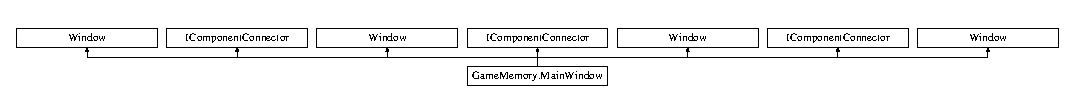
\includegraphics[height=0.919540cm]{class_game_memory_1_1_main_window}
\end{center}
\end{figure}
\subsection*{Public Member Functions}
\begin{DoxyCompactItemize}
\item 
void \hyperlink{class_game_memory_1_1_main_window_a830cbea78d6414fae17ccdb29f390824}{Set\-Master\-Table} ()
\item 
void \hyperlink{class_game_memory_1_1_main_window_abfbe514b8eb23764943a0b19ac00af0a}{Uninitialize\-Kinect\-Sensor} (Kinect\-Sensor kinect\-Sensor)
\item 
void \hyperlink{class_game_memory_1_1_main_window_ae2a1ab5e5ffc2383478ceaec18e83f51}{Initialize\-Component} ()
\begin{DoxyCompactList}\small\item\em Initialize\-Component \end{DoxyCompactList}\item 
void \hyperlink{class_game_memory_1_1_main_window_ae2a1ab5e5ffc2383478ceaec18e83f51}{Initialize\-Component} ()
\begin{DoxyCompactList}\small\item\em Initialize\-Component \end{DoxyCompactList}\item 
void \hyperlink{class_game_memory_1_1_main_window_ae2a1ab5e5ffc2383478ceaec18e83f51}{Initialize\-Component} ()
\begin{DoxyCompactList}\small\item\em Initialize\-Component \end{DoxyCompactList}\end{DoxyCompactItemize}
\subsection*{Properties}
\begin{DoxyCompactItemize}
\item 
\hypertarget{class_game_memory_1_1_main_window_ad741fff95ff7bcf760e6279fc2ff9107}{bool {\bfseries Has\-Active\-Skeleton}\hspace{0.3cm}{\ttfamily  \mbox{[}get, set\mbox{]}}}\label{class_game_memory_1_1_main_window_ad741fff95ff7bcf760e6279fc2ff9107}

\item 
\hypertarget{class_game_memory_1_1_main_window_a6a9aad72915b50bace61afe9ab55e0e5}{Kinect\-Sensor {\bfseries Kinect}\hspace{0.3cm}{\ttfamily  \mbox{[}get, set\mbox{]}}}\label{class_game_memory_1_1_main_window_a6a9aad72915b50bace61afe9ab55e0e5}

\end{DoxyCompactItemize}


\subsection{Detailed Description}
\hyperlink{class_game_memory_1_1_main_window}{Main\-Window} 

Class \hyperlink{class_game_memory_1_1_main_window}{Main\-Window}

\subsection{Member Function Documentation}
\hypertarget{class_game_memory_1_1_main_window_ae2a1ab5e5ffc2383478ceaec18e83f51}{\index{Game\-Memory\-::\-Main\-Window@{Game\-Memory\-::\-Main\-Window}!Initialize\-Component@{Initialize\-Component}}
\index{Initialize\-Component@{Initialize\-Component}!GameMemory::MainWindow@{Game\-Memory\-::\-Main\-Window}}
\subsubsection[{Initialize\-Component}]{\setlength{\rightskip}{0pt plus 5cm}void Game\-Memory.\-Main\-Window.\-Initialize\-Component (
\begin{DoxyParamCaption}
{}
\end{DoxyParamCaption}
)}}\label{class_game_memory_1_1_main_window_ae2a1ab5e5ffc2383478ceaec18e83f51}


Initialize\-Component 

\hypertarget{class_game_memory_1_1_main_window_ae2a1ab5e5ffc2383478ceaec18e83f51}{\index{Game\-Memory\-::\-Main\-Window@{Game\-Memory\-::\-Main\-Window}!Initialize\-Component@{Initialize\-Component}}
\index{Initialize\-Component@{Initialize\-Component}!GameMemory::MainWindow@{Game\-Memory\-::\-Main\-Window}}
\subsubsection[{Initialize\-Component}]{\setlength{\rightskip}{0pt plus 5cm}void Game\-Memory.\-Main\-Window.\-Initialize\-Component (
\begin{DoxyParamCaption}
{}
\end{DoxyParamCaption}
)}}\label{class_game_memory_1_1_main_window_ae2a1ab5e5ffc2383478ceaec18e83f51}


Initialize\-Component 

\hypertarget{class_game_memory_1_1_main_window_ae2a1ab5e5ffc2383478ceaec18e83f51}{\index{Game\-Memory\-::\-Main\-Window@{Game\-Memory\-::\-Main\-Window}!Initialize\-Component@{Initialize\-Component}}
\index{Initialize\-Component@{Initialize\-Component}!GameMemory::MainWindow@{Game\-Memory\-::\-Main\-Window}}
\subsubsection[{Initialize\-Component}]{\setlength{\rightskip}{0pt plus 5cm}void Game\-Memory.\-Main\-Window.\-Initialize\-Component (
\begin{DoxyParamCaption}
{}
\end{DoxyParamCaption}
)}}\label{class_game_memory_1_1_main_window_ae2a1ab5e5ffc2383478ceaec18e83f51}


Initialize\-Component 

\hypertarget{class_game_memory_1_1_main_window_a830cbea78d6414fae17ccdb29f390824}{\index{Game\-Memory\-::\-Main\-Window@{Game\-Memory\-::\-Main\-Window}!Set\-Master\-Table@{Set\-Master\-Table}}
\index{Set\-Master\-Table@{Set\-Master\-Table}!GameMemory::MainWindow@{Game\-Memory\-::\-Main\-Window}}
\subsubsection[{Set\-Master\-Table}]{\setlength{\rightskip}{0pt plus 5cm}void Game\-Memory.\-Main\-Window.\-Set\-Master\-Table (
\begin{DoxyParamCaption}
{}
\end{DoxyParamCaption}
)}}\label{class_game_memory_1_1_main_window_a830cbea78d6414fae17ccdb29f390824}
Inicializo las banderas de las vista y me gusta que va tener cada catálogo. \begin{DoxySince}{Since}
03/07/2012 
\end{DoxySince}
\hypertarget{class_game_memory_1_1_main_window_abfbe514b8eb23764943a0b19ac00af0a}{\index{Game\-Memory\-::\-Main\-Window@{Game\-Memory\-::\-Main\-Window}!Uninitialize\-Kinect\-Sensor@{Uninitialize\-Kinect\-Sensor}}
\index{Uninitialize\-Kinect\-Sensor@{Uninitialize\-Kinect\-Sensor}!GameMemory::MainWindow@{Game\-Memory\-::\-Main\-Window}}
\subsubsection[{Uninitialize\-Kinect\-Sensor}]{\setlength{\rightskip}{0pt plus 5cm}void Game\-Memory.\-Main\-Window.\-Uninitialize\-Kinect\-Sensor (
\begin{DoxyParamCaption}
\item[{Kinect\-Sensor}]{kinect\-Sensor}
\end{DoxyParamCaption}
)}}\label{class_game_memory_1_1_main_window_abfbe514b8eb23764943a0b19ac00af0a}
Method Uninitialize\-Kinect\-Sensor Detiene al sensor Kinect \begin{DoxySince}{Since}
17/06/2013 
\end{DoxySince}

\begin{DoxyParams}{Parameters}
{\em kinect\-Sensor} & Kinect\-Sensor \\
\hline
\end{DoxyParams}


The documentation for this class was generated from the following files\-:\begin{DoxyCompactItemize}
\item 
D\-:/tesis\-Assembla/branches/\-Branch\-\_\-\-Tesis\-\_\-\-Sprint01/\-Dev/\-Interaction Module/\-Game\-Memory/\-Game\-Memory/Main\-Window.\-xaml.\-cs\item 
D\-:/tesis\-Assembla/branches/\-Branch\-\_\-\-Tesis\-\_\-\-Sprint01/\-Dev/\-Interaction Module/\-Game\-Memory/\-Game\-Memory/obj/x86/\-Debug/Main\-Window.\-g.\-cs\item 
D\-:/tesis\-Assembla/branches/\-Branch\-\_\-\-Tesis\-\_\-\-Sprint01/\-Dev/\-Interaction Module/\-Game\-Memory/\-Game\-Memory/obj/x86/\-Debug/Main\-Window.\-g.\-i.\-cs\item 
D\-:/tesis\-Assembla/branches/\-Branch\-\_\-\-Tesis\-\_\-\-Sprint01/\-Dev/\-Interaction Module/\-Game\-Memory/\-Game\-Memory/obj/x86/\-Release/Main\-Window.\-g.\-i.\-cs\end{DoxyCompactItemize}

\hypertarget{class_game_memory_1_1_monitorings}{\section{Game\-Memory.\-Monitorings Class Reference}
\label{class_game_memory_1_1_monitorings}\index{Game\-Memory.\-Monitorings@{Game\-Memory.\-Monitorings}}
}


No hay documentación de metadatos disponible.  


Inheritance diagram for Game\-Memory.\-Monitorings\-:\begin{figure}[H]
\begin{center}
\leavevmode
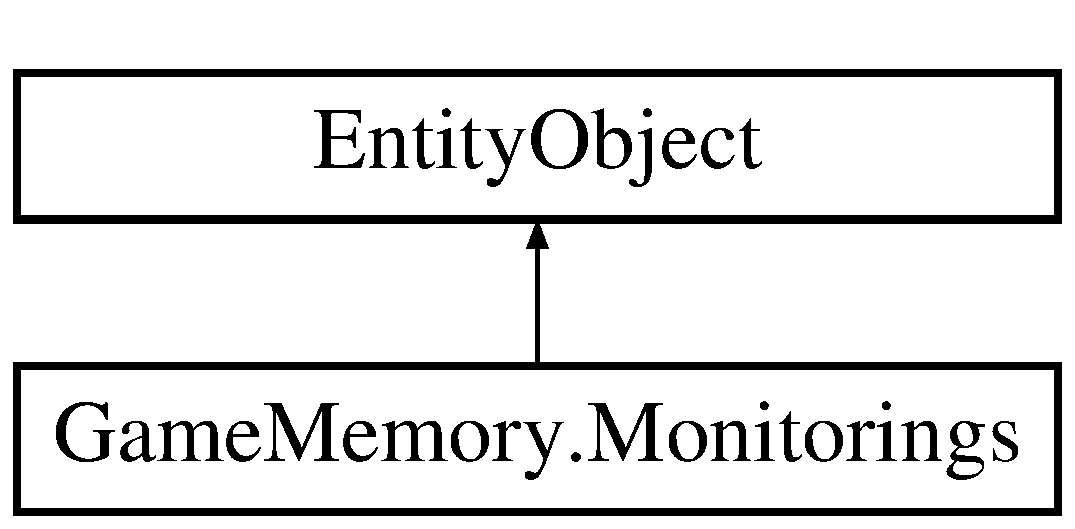
\includegraphics[height=2.000000cm]{class_game_memory_1_1_monitorings}
\end{center}
\end{figure}
\subsection*{Static Public Member Functions}
\begin{DoxyCompactItemize}
\item 
static \hyperlink{class_game_memory_1_1_monitorings}{Monitorings} \hyperlink{class_game_memory_1_1_monitorings_a6ba5e22e9d4a9030a9af1c33c0eb7627}{Create\-Monitorings} (global\-::\-System.\-Int32 monitoring\-I\-D, global\-::\-System.\-Int32 advert\-Host\-I\-D, global\-::\-System.\-Single average)
\begin{DoxyCompactList}\small\item\em Crear un nuevo objeto \hyperlink{class_game_memory_1_1_monitorings}{Monitorings}. \end{DoxyCompactList}\end{DoxyCompactItemize}
\subsection*{Properties}
\begin{DoxyCompactItemize}
\item 
global\-::\-System.\-Int32 \hyperlink{class_game_memory_1_1_monitorings_a26160580b6c9b96a7773135cec3a0409}{Monitoring\-I\-D}\hspace{0.3cm}{\ttfamily  \mbox{[}get, set\mbox{]}}
\begin{DoxyCompactList}\small\item\em No hay documentación de metadatos disponible. \end{DoxyCompactList}\item 
global\-::\-System.\-Int32 \hyperlink{class_game_memory_1_1_monitorings_af6570a77b6f0cc4a462e4421ce5f913c}{Advert\-Host\-I\-D}\hspace{0.3cm}{\ttfamily  \mbox{[}get, set\mbox{]}}
\begin{DoxyCompactList}\small\item\em No hay documentación de metadatos disponible. \end{DoxyCompactList}\item 
Nullable$<$ global\-::\-System.\-Date\-Time $>$ \hyperlink{class_game_memory_1_1_monitorings_aa2aab4600abf54e97998d55a8c6a7520}{Timestamp}\hspace{0.3cm}{\ttfamily  \mbox{[}get, set\mbox{]}}
\begin{DoxyCompactList}\small\item\em No hay documentación de metadatos disponible. \end{DoxyCompactList}\item 
global\-::\-System.\-Single \hyperlink{class_game_memory_1_1_monitorings_a7e93e01d5c9831e48213a03aa37ac386}{Average}\hspace{0.3cm}{\ttfamily  \mbox{[}get, set\mbox{]}}
\begin{DoxyCompactList}\small\item\em No hay documentación de metadatos disponible. \end{DoxyCompactList}\item 
\hyperlink{class_game_memory_1_1_advert_hosts}{Advert\-Hosts} \hyperlink{class_game_memory_1_1_monitorings_a10100dcedb82f94509cc9e9c62c25db5}{Advert\-Hosts}\hspace{0.3cm}{\ttfamily  \mbox{[}get, set\mbox{]}}
\begin{DoxyCompactList}\small\item\em No hay documentación de metadatos disponible. \end{DoxyCompactList}\item 
Entity\-Reference$<$ \hyperlink{class_game_memory_1_1_advert_hosts}{Advert\-Hosts} $>$ \hyperlink{class_game_memory_1_1_monitorings_aac0e39b01bbc04291109a4d934708151}{Advert\-Hosts\-Reference}\hspace{0.3cm}{\ttfamily  \mbox{[}get, set\mbox{]}}
\begin{DoxyCompactList}\small\item\em No hay documentación de metadatos disponible. \end{DoxyCompactList}\end{DoxyCompactItemize}


\subsection{Detailed Description}
No hay documentación de metadatos disponible. 



\subsection{Member Function Documentation}
\hypertarget{class_game_memory_1_1_monitorings_a6ba5e22e9d4a9030a9af1c33c0eb7627}{\index{Game\-Memory\-::\-Monitorings@{Game\-Memory\-::\-Monitorings}!Create\-Monitorings@{Create\-Monitorings}}
\index{Create\-Monitorings@{Create\-Monitorings}!GameMemory::Monitorings@{Game\-Memory\-::\-Monitorings}}
\subsubsection[{Create\-Monitorings}]{\setlength{\rightskip}{0pt plus 5cm}static {\bf Monitorings} Game\-Memory.\-Monitorings.\-Create\-Monitorings (
\begin{DoxyParamCaption}
\item[{global\-::\-System.\-Int32}]{monitoring\-I\-D, }
\item[{global\-::\-System.\-Int32}]{advert\-Host\-I\-D, }
\item[{global\-::\-System.\-Single}]{average}
\end{DoxyParamCaption}
)\hspace{0.3cm}{\ttfamily [static]}}}\label{class_game_memory_1_1_monitorings_a6ba5e22e9d4a9030a9af1c33c0eb7627}


Crear un nuevo objeto \hyperlink{class_game_memory_1_1_monitorings}{Monitorings}. 


\begin{DoxyParams}{Parameters}
{\em monitoring\-I\-D} & Valor inicial de la propiedad Monitoring\-I\-D.\\
\hline
{\em advert\-Host\-I\-D} & Valor inicial de la propiedad Advert\-Host\-I\-D.\\
\hline
{\em average} & Valor inicial de la propiedad Average.\\
\hline
\end{DoxyParams}


\subsection{Property Documentation}
\hypertarget{class_game_memory_1_1_monitorings_af6570a77b6f0cc4a462e4421ce5f913c}{\index{Game\-Memory\-::\-Monitorings@{Game\-Memory\-::\-Monitorings}!Advert\-Host\-I\-D@{Advert\-Host\-I\-D}}
\index{Advert\-Host\-I\-D@{Advert\-Host\-I\-D}!GameMemory::Monitorings@{Game\-Memory\-::\-Monitorings}}
\subsubsection[{Advert\-Host\-I\-D}]{\setlength{\rightskip}{0pt plus 5cm}global.\-System.\-Int32 Game\-Memory.\-Monitorings.\-Advert\-Host\-I\-D\hspace{0.3cm}{\ttfamily [get]}, {\ttfamily [set]}}}\label{class_game_memory_1_1_monitorings_af6570a77b6f0cc4a462e4421ce5f913c}


No hay documentación de metadatos disponible. 

\hypertarget{class_game_memory_1_1_monitorings_a10100dcedb82f94509cc9e9c62c25db5}{\index{Game\-Memory\-::\-Monitorings@{Game\-Memory\-::\-Monitorings}!Advert\-Hosts@{Advert\-Hosts}}
\index{Advert\-Hosts@{Advert\-Hosts}!GameMemory::Monitorings@{Game\-Memory\-::\-Monitorings}}
\subsubsection[{Advert\-Hosts}]{\setlength{\rightskip}{0pt plus 5cm}{\bf Advert\-Hosts} Game\-Memory.\-Monitorings.\-Advert\-Hosts\hspace{0.3cm}{\ttfamily [get]}, {\ttfamily [set]}}}\label{class_game_memory_1_1_monitorings_a10100dcedb82f94509cc9e9c62c25db5}


No hay documentación de metadatos disponible. 

\hypertarget{class_game_memory_1_1_monitorings_aac0e39b01bbc04291109a4d934708151}{\index{Game\-Memory\-::\-Monitorings@{Game\-Memory\-::\-Monitorings}!Advert\-Hosts\-Reference@{Advert\-Hosts\-Reference}}
\index{Advert\-Hosts\-Reference@{Advert\-Hosts\-Reference}!GameMemory::Monitorings@{Game\-Memory\-::\-Monitorings}}
\subsubsection[{Advert\-Hosts\-Reference}]{\setlength{\rightskip}{0pt plus 5cm}Entity\-Reference$<${\bf Advert\-Hosts}$>$ Game\-Memory.\-Monitorings.\-Advert\-Hosts\-Reference\hspace{0.3cm}{\ttfamily [get]}, {\ttfamily [set]}}}\label{class_game_memory_1_1_monitorings_aac0e39b01bbc04291109a4d934708151}


No hay documentación de metadatos disponible. 

\hypertarget{class_game_memory_1_1_monitorings_a7e93e01d5c9831e48213a03aa37ac386}{\index{Game\-Memory\-::\-Monitorings@{Game\-Memory\-::\-Monitorings}!Average@{Average}}
\index{Average@{Average}!GameMemory::Monitorings@{Game\-Memory\-::\-Monitorings}}
\subsubsection[{Average}]{\setlength{\rightskip}{0pt plus 5cm}global.\-System.\-Single Game\-Memory.\-Monitorings.\-Average\hspace{0.3cm}{\ttfamily [get]}, {\ttfamily [set]}}}\label{class_game_memory_1_1_monitorings_a7e93e01d5c9831e48213a03aa37ac386}


No hay documentación de metadatos disponible. 

\hypertarget{class_game_memory_1_1_monitorings_a26160580b6c9b96a7773135cec3a0409}{\index{Game\-Memory\-::\-Monitorings@{Game\-Memory\-::\-Monitorings}!Monitoring\-I\-D@{Monitoring\-I\-D}}
\index{Monitoring\-I\-D@{Monitoring\-I\-D}!GameMemory::Monitorings@{Game\-Memory\-::\-Monitorings}}
\subsubsection[{Monitoring\-I\-D}]{\setlength{\rightskip}{0pt plus 5cm}global.\-System.\-Int32 Game\-Memory.\-Monitorings.\-Monitoring\-I\-D\hspace{0.3cm}{\ttfamily [get]}, {\ttfamily [set]}}}\label{class_game_memory_1_1_monitorings_a26160580b6c9b96a7773135cec3a0409}


No hay documentación de metadatos disponible. 

\hypertarget{class_game_memory_1_1_monitorings_aa2aab4600abf54e97998d55a8c6a7520}{\index{Game\-Memory\-::\-Monitorings@{Game\-Memory\-::\-Monitorings}!Timestamp@{Timestamp}}
\index{Timestamp@{Timestamp}!GameMemory::Monitorings@{Game\-Memory\-::\-Monitorings}}
\subsubsection[{Timestamp}]{\setlength{\rightskip}{0pt plus 5cm}Nullable$<$global.\-System.\-Date\-Time$>$ Game\-Memory.\-Monitorings.\-Timestamp\hspace{0.3cm}{\ttfamily [get]}, {\ttfamily [set]}}}\label{class_game_memory_1_1_monitorings_aa2aab4600abf54e97998d55a8c6a7520}


No hay documentación de metadatos disponible. 



The documentation for this class was generated from the following file\-:\begin{DoxyCompactItemize}
\item 
D\-:/tesis\-Assembla/branches/\-Branch\-\_\-\-Tesis\-\_\-\-Sprint01/\-Dev/\-Interaction Module/\-Game\-Memory/\-Game\-Memory/O\-M\-K\-T.\-Designer.\-cs\end{DoxyCompactItemize}

\hypertarget{class_game_memory_1_1_networks}{\section{Game\-Memory.\-Networks Class Reference}
\label{class_game_memory_1_1_networks}\index{Game\-Memory.\-Networks@{Game\-Memory.\-Networks}}
}


No hay documentación de metadatos disponible.  


Inheritance diagram for Game\-Memory.\-Networks\-:\begin{figure}[H]
\begin{center}
\leavevmode
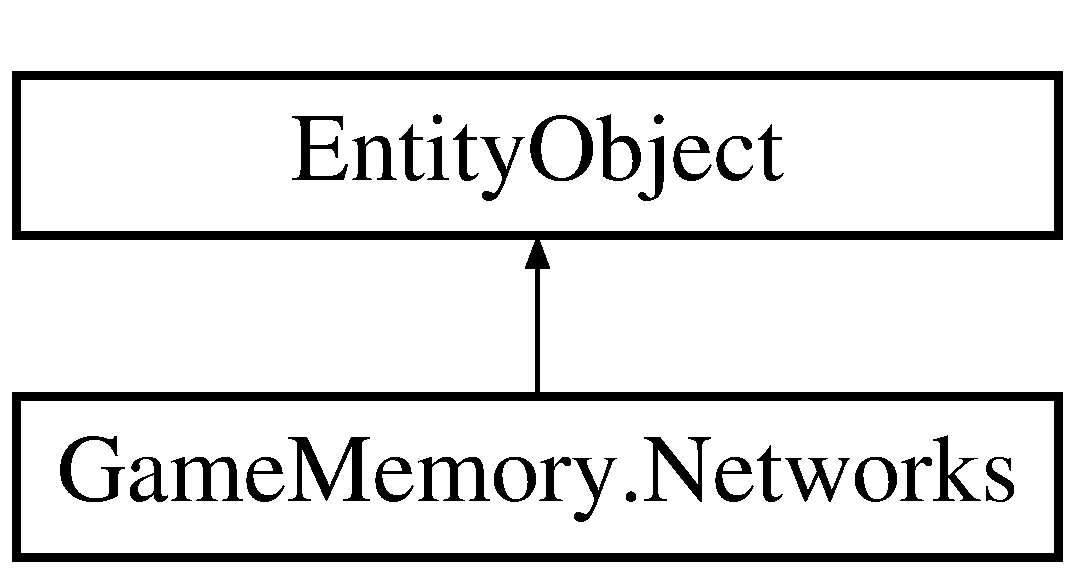
\includegraphics[height=2.000000cm]{class_game_memory_1_1_networks}
\end{center}
\end{figure}
\subsection*{Static Public Member Functions}
\begin{DoxyCompactItemize}
\item 
static \hyperlink{class_game_memory_1_1_networks}{Networks} \hyperlink{class_game_memory_1_1_networks_a5e6c60874478cc5e562636f623c7e5a9}{Create\-Networks} (global\-::\-System.\-Int32 network\-Id)
\begin{DoxyCompactList}\small\item\em Crear un nuevo objeto \hyperlink{class_game_memory_1_1_networks}{Networks}. \end{DoxyCompactList}\end{DoxyCompactItemize}
\subsection*{Properties}
\begin{DoxyCompactItemize}
\item 
global\-::\-System.\-Int32 \hyperlink{class_game_memory_1_1_networks_a111b12af812530cd931a0a094db04d01}{Network\-Id}\hspace{0.3cm}{\ttfamily  \mbox{[}get, set\mbox{]}}
\begin{DoxyCompactList}\small\item\em No hay documentación de metadatos disponible. \end{DoxyCompactList}\item 
global\-::\-System.\-String \hyperlink{class_game_memory_1_1_networks_a0d21cf294bbf9f1be6d0d43875997ba3}{Description}\hspace{0.3cm}{\ttfamily  \mbox{[}get, set\mbox{]}}
\begin{DoxyCompactList}\small\item\em No hay documentación de metadatos disponible. \end{DoxyCompactList}\item 
Entity\-Collection$<$ \hyperlink{class_game_memory_1_1_advert_campaigns}{Advert\-Campaigns} $>$ \hyperlink{class_game_memory_1_1_networks_aeff3d628f46ff88b75b6c8560965690d}{Advert\-Campaigns}\hspace{0.3cm}{\ttfamily  \mbox{[}get, set\mbox{]}}
\begin{DoxyCompactList}\small\item\em No hay documentación de metadatos disponible. \end{DoxyCompactList}\end{DoxyCompactItemize}


\subsection{Detailed Description}
No hay documentación de metadatos disponible. 



\subsection{Member Function Documentation}
\hypertarget{class_game_memory_1_1_networks_a5e6c60874478cc5e562636f623c7e5a9}{\index{Game\-Memory\-::\-Networks@{Game\-Memory\-::\-Networks}!Create\-Networks@{Create\-Networks}}
\index{Create\-Networks@{Create\-Networks}!GameMemory::Networks@{Game\-Memory\-::\-Networks}}
\subsubsection[{Create\-Networks}]{\setlength{\rightskip}{0pt plus 5cm}static {\bf Networks} Game\-Memory.\-Networks.\-Create\-Networks (
\begin{DoxyParamCaption}
\item[{global\-::\-System.\-Int32}]{network\-Id}
\end{DoxyParamCaption}
)\hspace{0.3cm}{\ttfamily [static]}}}\label{class_game_memory_1_1_networks_a5e6c60874478cc5e562636f623c7e5a9}


Crear un nuevo objeto \hyperlink{class_game_memory_1_1_networks}{Networks}. 


\begin{DoxyParams}{Parameters}
{\em network\-Id} & Valor inicial de la propiedad Network\-Id.\\
\hline
\end{DoxyParams}


\subsection{Property Documentation}
\hypertarget{class_game_memory_1_1_networks_aeff3d628f46ff88b75b6c8560965690d}{\index{Game\-Memory\-::\-Networks@{Game\-Memory\-::\-Networks}!Advert\-Campaigns@{Advert\-Campaigns}}
\index{Advert\-Campaigns@{Advert\-Campaigns}!GameMemory::Networks@{Game\-Memory\-::\-Networks}}
\subsubsection[{Advert\-Campaigns}]{\setlength{\rightskip}{0pt plus 5cm}Entity\-Collection$<${\bf Advert\-Campaigns}$>$ Game\-Memory.\-Networks.\-Advert\-Campaigns\hspace{0.3cm}{\ttfamily [get]}, {\ttfamily [set]}}}\label{class_game_memory_1_1_networks_aeff3d628f46ff88b75b6c8560965690d}


No hay documentación de metadatos disponible. 

\hypertarget{class_game_memory_1_1_networks_a0d21cf294bbf9f1be6d0d43875997ba3}{\index{Game\-Memory\-::\-Networks@{Game\-Memory\-::\-Networks}!Description@{Description}}
\index{Description@{Description}!GameMemory::Networks@{Game\-Memory\-::\-Networks}}
\subsubsection[{Description}]{\setlength{\rightskip}{0pt plus 5cm}global.\-System.\-String Game\-Memory.\-Networks.\-Description\hspace{0.3cm}{\ttfamily [get]}, {\ttfamily [set]}}}\label{class_game_memory_1_1_networks_a0d21cf294bbf9f1be6d0d43875997ba3}


No hay documentación de metadatos disponible. 

\hypertarget{class_game_memory_1_1_networks_a111b12af812530cd931a0a094db04d01}{\index{Game\-Memory\-::\-Networks@{Game\-Memory\-::\-Networks}!Network\-Id@{Network\-Id}}
\index{Network\-Id@{Network\-Id}!GameMemory::Networks@{Game\-Memory\-::\-Networks}}
\subsubsection[{Network\-Id}]{\setlength{\rightskip}{0pt plus 5cm}global.\-System.\-Int32 Game\-Memory.\-Networks.\-Network\-Id\hspace{0.3cm}{\ttfamily [get]}, {\ttfamily [set]}}}\label{class_game_memory_1_1_networks_a111b12af812530cd931a0a094db04d01}


No hay documentación de metadatos disponible. 



The documentation for this class was generated from the following file\-:\begin{DoxyCompactItemize}
\item 
D\-:/tesis\-Assembla/branches/\-Branch\-\_\-\-Tesis\-\_\-\-Sprint01/\-Dev/\-Interaction Module/\-Game\-Memory/\-Game\-Memory/O\-M\-K\-T.\-Designer.\-cs\end{DoxyCompactItemize}

\hypertarget{class_game_memory_1_1_o_m_k_t_d_b_entities}{\section{Game\-Memory.\-O\-M\-K\-T\-D\-B\-Entities Class Reference}
\label{class_game_memory_1_1_o_m_k_t_d_b_entities}\index{Game\-Memory.\-O\-M\-K\-T\-D\-B\-Entities@{Game\-Memory.\-O\-M\-K\-T\-D\-B\-Entities}}
}


No hay documentación de metadatos disponible.  


Inheritance diagram for Game\-Memory.\-O\-M\-K\-T\-D\-B\-Entities\-:\begin{figure}[H]
\begin{center}
\leavevmode
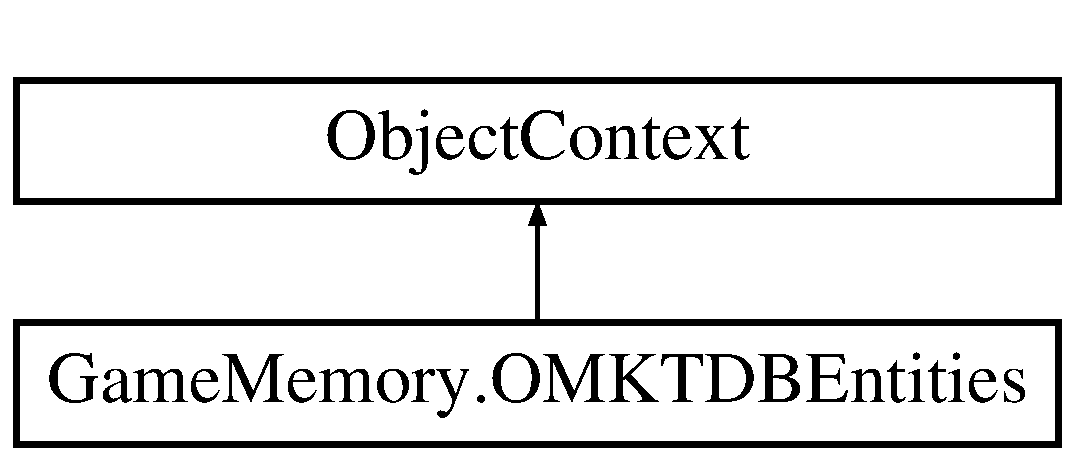
\includegraphics[height=2.000000cm]{class_game_memory_1_1_o_m_k_t_d_b_entities}
\end{center}
\end{figure}
\subsection*{Public Member Functions}
\begin{DoxyCompactItemize}
\item 
\hyperlink{class_game_memory_1_1_o_m_k_t_d_b_entities_a0aafc6eff88094ee3298696afb1f379a}{O\-M\-K\-T\-D\-B\-Entities} ()
\begin{DoxyCompactList}\small\item\em Inicializa un nuevo objeto \hyperlink{class_game_memory_1_1_o_m_k_t_d_b_entities}{O\-M\-K\-T\-D\-B\-Entities} usando la cadena de conexión encontrada en la sección '\hyperlink{class_game_memory_1_1_o_m_k_t_d_b_entities}{O\-M\-K\-T\-D\-B\-Entities}' del archivo de configuración de la aplicación. \end{DoxyCompactList}\item 
\hyperlink{class_game_memory_1_1_o_m_k_t_d_b_entities_a176e56526c22b56f058e0e5558003549}{O\-M\-K\-T\-D\-B\-Entities} (string connection\-String)
\begin{DoxyCompactList}\small\item\em Inicializar un nuevo objeto \hyperlink{class_game_memory_1_1_o_m_k_t_d_b_entities}{O\-M\-K\-T\-D\-B\-Entities}. \end{DoxyCompactList}\item 
\hyperlink{class_game_memory_1_1_o_m_k_t_d_b_entities_a402c8c5e03fbf49df4efc864096c7de9}{O\-M\-K\-T\-D\-B\-Entities} (Entity\-Connection connection)
\begin{DoxyCompactList}\small\item\em Inicializar un nuevo objeto \hyperlink{class_game_memory_1_1_o_m_k_t_d_b_entities}{O\-M\-K\-T\-D\-B\-Entities}. \end{DoxyCompactList}\item 
void \hyperlink{class_game_memory_1_1_o_m_k_t_d_b_entities_a61799ab7889066b0cb44d3e67d25a7ee}{Add\-To\-C\-\_\-\-\_\-\-Migration\-History} (\hyperlink{class_game_memory_1_1_c_____migration_history}{C\-\_\-\-\_\-\-Migration\-History} c\-\_\-\-\_\-\-Migration\-History)
\begin{DoxyCompactList}\small\item\em Método desusado para agregar un nuevo objeto al Entity\-Set \hyperlink{class_game_memory_1_1_c_____migration_history}{C\-\_\-\-\_\-\-Migration\-History}. Considere la posibilidad de usar el método .Add de la propiedad Object\-Set$<$T$>$ asociada. \end{DoxyCompactList}\item 
void \hyperlink{class_game_memory_1_1_o_m_k_t_d_b_entities_a2b013b78ec8bc9c3598a86d1c7f5b06f}{Add\-To\-Advert\-Campaign\-Detail\-Interactions} (\hyperlink{class_game_memory_1_1_advert_campaign_detail_interactions}{Advert\-Campaign\-Detail\-Interactions} advert\-Campaign\-Detail\-Interactions)
\begin{DoxyCompactList}\small\item\em Método desusado para agregar un nuevo objeto al Entity\-Set \hyperlink{class_game_memory_1_1_advert_campaign_detail_interactions}{Advert\-Campaign\-Detail\-Interactions}. Considere la posibilidad de usar el método .Add de la propiedad Object\-Set$<$T$>$ asociada. \end{DoxyCompactList}\item 
void \hyperlink{class_game_memory_1_1_o_m_k_t_d_b_entities_a2a1ff115c82b822436dfc177b47d2523}{Add\-To\-Advert\-Campaign\-Details} (\hyperlink{class_game_memory_1_1_advert_campaign_details}{Advert\-Campaign\-Details} advert\-Campaign\-Details)
\begin{DoxyCompactList}\small\item\em Método desusado para agregar un nuevo objeto al Entity\-Set \hyperlink{class_game_memory_1_1_advert_campaign_details}{Advert\-Campaign\-Details}. Considere la posibilidad de usar el método .Add de la propiedad Object\-Set$<$T$>$ asociada. \end{DoxyCompactList}\item 
void \hyperlink{class_game_memory_1_1_o_m_k_t_d_b_entities_a44fb4c2c2cd41a93cc34dddc16cd4071}{Add\-To\-Advert\-Campaign\-Interactions} (\hyperlink{class_game_memory_1_1_advert_campaign_interactions}{Advert\-Campaign\-Interactions} advert\-Campaign\-Interactions)
\begin{DoxyCompactList}\small\item\em Método desusado para agregar un nuevo objeto al Entity\-Set \hyperlink{class_game_memory_1_1_advert_campaign_interactions}{Advert\-Campaign\-Interactions}. Considere la posibilidad de usar el método .Add de la propiedad Object\-Set$<$T$>$ asociada. \end{DoxyCompactList}\item 
void \hyperlink{class_game_memory_1_1_o_m_k_t_d_b_entities_a9a897797208a4e7187c478d9fe9f90b7}{Add\-To\-Advert\-Campaigns} (\hyperlink{class_game_memory_1_1_advert_campaigns}{Advert\-Campaigns} advert\-Campaigns)
\begin{DoxyCompactList}\small\item\em Método desusado para agregar un nuevo objeto al Entity\-Set \hyperlink{class_game_memory_1_1_advert_campaigns}{Advert\-Campaigns}. Considere la posibilidad de usar el método .Add de la propiedad Object\-Set$<$T$>$ asociada. \end{DoxyCompactList}\item 
void \hyperlink{class_game_memory_1_1_o_m_k_t_d_b_entities_a6639f5f52306d0ffd29181498836a880}{Add\-To\-Advert\-Host\-Categories} (\hyperlink{class_game_memory_1_1_advert_host_categories}{Advert\-Host\-Categories} advert\-Host\-Categories)
\begin{DoxyCompactList}\small\item\em Método desusado para agregar un nuevo objeto al Entity\-Set \hyperlink{class_game_memory_1_1_advert_host_categories}{Advert\-Host\-Categories}. Considere la posibilidad de usar el método .Add de la propiedad Object\-Set$<$T$>$ asociada. \end{DoxyCompactList}\item 
void \hyperlink{class_game_memory_1_1_o_m_k_t_d_b_entities_a882936b1bc8f11bf17d5532727d03c5b}{Add\-To\-Advert\-Hosts} (\hyperlink{class_game_memory_1_1_advert_hosts}{Advert\-Hosts} advert\-Hosts)
\begin{DoxyCompactList}\small\item\em Método desusado para agregar un nuevo objeto al Entity\-Set \hyperlink{class_game_memory_1_1_advert_hosts}{Advert\-Hosts}. Considere la posibilidad de usar el método .Add de la propiedad Object\-Set$<$T$>$ asociada. \end{DoxyCompactList}\item 
void \hyperlink{class_game_memory_1_1_o_m_k_t_d_b_entities_a141864354b614abef2757fefd2371116}{Add\-To\-Adverts} (\hyperlink{class_game_memory_1_1_adverts}{Adverts} adverts)
\begin{DoxyCompactList}\small\item\em Método desusado para agregar un nuevo objeto al Entity\-Set \hyperlink{class_game_memory_1_1_adverts}{Adverts}. Considere la posibilidad de usar el método .Add de la propiedad Object\-Set$<$T$>$ asociada. \end{DoxyCompactList}\item 
void \hyperlink{class_game_memory_1_1_o_m_k_t_d_b_entities_a89018467bbc55317db078f162456ce38}{Add\-To\-Advert\-States} (\hyperlink{class_game_memory_1_1_advert_states}{Advert\-States} advert\-States)
\begin{DoxyCompactList}\small\item\em Método desusado para agregar un nuevo objeto al Entity\-Set \hyperlink{class_game_memory_1_1_advert_states}{Advert\-States}. Considere la posibilidad de usar el método .Add de la propiedad Object\-Set$<$T$>$ asociada. \end{DoxyCompactList}\item 
void \hyperlink{class_game_memory_1_1_o_m_k_t_d_b_entities_a5285be4f02b9c7b324966a09f376f09e}{Add\-To\-Advert\-Types} (\hyperlink{class_game_memory_1_1_advert_types}{Advert\-Types} advert\-Types)
\begin{DoxyCompactList}\small\item\em Método desusado para agregar un nuevo objeto al Entity\-Set \hyperlink{class_game_memory_1_1_advert_types}{Advert\-Types}. Considere la posibilidad de usar el método .Add de la propiedad Object\-Set$<$T$>$ asociada. \end{DoxyCompactList}\item 
void \hyperlink{class_game_memory_1_1_o_m_k_t_d_b_entities_aedcaf52099af392ca22539bde2cc076e}{Add\-To\-Alerts} (\hyperlink{class_game_memory_1_1_alerts}{Alerts} alerts)
\begin{DoxyCompactList}\small\item\em Método desusado para agregar un nuevo objeto al Entity\-Set \hyperlink{class_game_memory_1_1_alerts}{Alerts}. Considere la posibilidad de usar el método .Add de la propiedad Object\-Set$<$T$>$ asociada. \end{DoxyCompactList}\item 
void \hyperlink{class_game_memory_1_1_o_m_k_t_d_b_entities_af4cf8e74e5269f08f58daab1201c3249}{Add\-To\-Campaign\-Locations} (\hyperlink{class_game_memory_1_1_campaign_locations}{Campaign\-Locations} campaign\-Locations)
\begin{DoxyCompactList}\small\item\em Método desusado para agregar un nuevo objeto al Entity\-Set \hyperlink{class_game_memory_1_1_campaign_locations}{Campaign\-Locations}. Considere la posibilidad de usar el método .Add de la propiedad Object\-Set$<$T$>$ asociada. \end{DoxyCompactList}\item 
void \hyperlink{class_game_memory_1_1_o_m_k_t_d_b_entities_af2a779d319fae157b8b2be8929457eb8}{Add\-To\-Campaign\-States} (\hyperlink{class_game_memory_1_1_campaign_states}{Campaign\-States} campaign\-States)
\begin{DoxyCompactList}\small\item\em Método desusado para agregar un nuevo objeto al Entity\-Set \hyperlink{class_game_memory_1_1_campaign_states}{Campaign\-States}. Considere la posibilidad de usar el método .Add de la propiedad Object\-Set$<$T$>$ asociada. \end{DoxyCompactList}\item 
void \hyperlink{class_game_memory_1_1_o_m_k_t_d_b_entities_ab0fab6d7cf71c0ecc1ebedbc678211fb}{Add\-To\-Campaign\-Types} (\hyperlink{class_game_memory_1_1_campaign_types}{Campaign\-Types} campaign\-Types)
\begin{DoxyCompactList}\small\item\em Método desusado para agregar un nuevo objeto al Entity\-Set \hyperlink{class_game_memory_1_1_campaign_types}{Campaign\-Types}. Considere la posibilidad de usar el método .Add de la propiedad Object\-Set$<$T$>$ asociada. \end{DoxyCompactList}\item 
void \hyperlink{class_game_memory_1_1_o_m_k_t_d_b_entities_abb21e3cf4428cb1d6d85685e10b973c4}{Add\-To\-Catalog\-Detail\-Interactions} (\hyperlink{class_game_memory_1_1_catalog_detail_interactions}{Catalog\-Detail\-Interactions} catalog\-Detail\-Interactions)
\begin{DoxyCompactList}\small\item\em Método desusado para agregar un nuevo objeto al Entity\-Set \hyperlink{class_game_memory_1_1_catalog_detail_interactions}{Catalog\-Detail\-Interactions}. Considere la posibilidad de usar el método .Add de la propiedad Object\-Set$<$T$>$ asociada. \end{DoxyCompactList}\item 
void \hyperlink{class_game_memory_1_1_o_m_k_t_d_b_entities_a64cd8667b4656b326a730d8fa864050e}{Add\-To\-Catalog\-Details} (\hyperlink{class_game_memory_1_1_catalog_details}{Catalog\-Details} catalog\-Details)
\begin{DoxyCompactList}\small\item\em Método desusado para agregar un nuevo objeto al Entity\-Set \hyperlink{class_game_memory_1_1_catalog_details}{Catalog\-Details}. Considere la posibilidad de usar el método .Add de la propiedad Object\-Set$<$T$>$ asociada. \end{DoxyCompactList}\item 
void \hyperlink{class_game_memory_1_1_o_m_k_t_d_b_entities_aa04f123e04bb601e9b114809de7e75b7}{Add\-To\-Commercial\-Products} (\hyperlink{class_game_memory_1_1_commercial_products}{Commercial\-Products} commercial\-Products)
\begin{DoxyCompactList}\small\item\em Método desusado para agregar un nuevo objeto al Entity\-Set \hyperlink{class_game_memory_1_1_commercial_products}{Commercial\-Products}. Considere la posibilidad de usar el método .Add de la propiedad Object\-Set$<$T$>$ asociada. \end{DoxyCompactList}\item 
void \hyperlink{class_game_memory_1_1_o_m_k_t_d_b_entities_a2e9e997768e7ede8269216f36b7bc8c1}{Add\-To\-Commercial\-Product\-Types} (\hyperlink{class_game_memory_1_1_commercial_product_types}{Commercial\-Product\-Types} commercial\-Product\-Types)
\begin{DoxyCompactList}\small\item\em Método desusado para agregar un nuevo objeto al Entity\-Set \hyperlink{class_game_memory_1_1_commercial_product_types}{Commercial\-Product\-Types}. Considere la posibilidad de usar el método .Add de la propiedad Object\-Set$<$T$>$ asociada. \end{DoxyCompactList}\item 
void \hyperlink{class_game_memory_1_1_o_m_k_t_d_b_entities_ac35584f2d5718386fb999d2215ee4e7d}{Add\-To\-Customers} (\hyperlink{class_game_memory_1_1_customers}{Customers} customers)
\begin{DoxyCompactList}\small\item\em Método desusado para agregar un nuevo objeto al Entity\-Set \hyperlink{class_game_memory_1_1_customers}{Customers}. Considere la posibilidad de usar el método .Add de la propiedad Object\-Set$<$T$>$ asociada. \end{DoxyCompactList}\item 
void \hyperlink{class_game_memory_1_1_o_m_k_t_d_b_entities_abd0a178b54323dd14425c06ed4ae002f}{Add\-To\-Game\-Detail\-Interactions} (\hyperlink{class_game_memory_1_1_game_detail_interactions}{Game\-Detail\-Interactions} game\-Detail\-Interactions)
\begin{DoxyCompactList}\small\item\em Método desusado para agregar un nuevo objeto al Entity\-Set \hyperlink{class_game_memory_1_1_game_detail_interactions}{Game\-Detail\-Interactions}. Considere la posibilidad de usar el método .Add de la propiedad Object\-Set$<$T$>$ asociada. \end{DoxyCompactList}\item 
void \hyperlink{class_game_memory_1_1_o_m_k_t_d_b_entities_a0e4422cc4f67163ef8d56970b295dd45}{Add\-To\-Game\-Details} (\hyperlink{class_game_memory_1_1_game_details}{Game\-Details} game\-Details)
\begin{DoxyCompactList}\small\item\em Método desusado para agregar un nuevo objeto al Entity\-Set \hyperlink{class_game_memory_1_1_game_details}{Game\-Details}. Considere la posibilidad de usar el método .Add de la propiedad Object\-Set$<$T$>$ asociada. \end{DoxyCompactList}\item 
void \hyperlink{class_game_memory_1_1_o_m_k_t_d_b_entities_aa77570b2e4a8cfb400959bd8045a6264}{Add\-To\-Inboxes} (\hyperlink{class_game_memory_1_1_inboxes}{Inboxes} inboxes)
\begin{DoxyCompactList}\small\item\em Método desusado para agregar un nuevo objeto al Entity\-Set \hyperlink{class_game_memory_1_1_inboxes}{Inboxes}. Considere la posibilidad de usar el método .Add de la propiedad Object\-Set$<$T$>$ asociada. \end{DoxyCompactList}\item 
void \hyperlink{class_game_memory_1_1_o_m_k_t_d_b_entities_ace4f60560edc5ffa1f4cb00adfcbd2da}{Add\-To\-Interactions} (\hyperlink{class_game_memory_1_1_interactions}{Interactions} interactions)
\begin{DoxyCompactList}\small\item\em Método desusado para agregar un nuevo objeto al Entity\-Set \hyperlink{class_game_memory_1_1_interactions}{Interactions}. Considere la posibilidad de usar el método .Add de la propiedad Object\-Set$<$T$>$ asociada. \end{DoxyCompactList}\item 
void \hyperlink{class_game_memory_1_1_o_m_k_t_d_b_entities_ab288fd2c58e6f298a4c74b584b82f060}{Add\-To\-Invoice\-Details} (\hyperlink{class_game_memory_1_1_invoice_details}{Invoice\-Details} invoice\-Details)
\begin{DoxyCompactList}\small\item\em Método desusado para agregar un nuevo objeto al Entity\-Set \hyperlink{class_game_memory_1_1_invoice_details}{Invoice\-Details}. Considere la posibilidad de usar el método .Add de la propiedad Object\-Set$<$T$>$ asociada. \end{DoxyCompactList}\item 
void \hyperlink{class_game_memory_1_1_o_m_k_t_d_b_entities_a0ce70d69289c3488b6f582ed60f5ec58}{Add\-To\-Invoices} (\hyperlink{class_game_memory_1_1_invoices}{Invoices} invoices)
\begin{DoxyCompactList}\small\item\em Método desusado para agregar un nuevo objeto al Entity\-Set \hyperlink{class_game_memory_1_1_invoices}{Invoices}. Considere la posibilidad de usar el método .Add de la propiedad Object\-Set$<$T$>$ asociada. \end{DoxyCompactList}\item 
void \hyperlink{class_game_memory_1_1_o_m_k_t_d_b_entities_a3c25b648c0400245ff6ca894c073fcbb}{Add\-To\-Locations} (\hyperlink{class_game_memory_1_1_locations}{Locations} locations)
\begin{DoxyCompactList}\small\item\em Método desusado para agregar un nuevo objeto al Entity\-Set \hyperlink{class_game_memory_1_1_locations}{Locations}. Considere la posibilidad de usar el método .Add de la propiedad Object\-Set$<$T$>$ asociada. \end{DoxyCompactList}\item 
void \hyperlink{class_game_memory_1_1_o_m_k_t_d_b_entities_a8a56f9ac74083756b2011a43e65b311c}{Add\-To\-Monitorings} (\hyperlink{class_game_memory_1_1_monitorings}{Monitorings} monitorings)
\begin{DoxyCompactList}\small\item\em Método desusado para agregar un nuevo objeto al Entity\-Set \hyperlink{class_game_memory_1_1_monitorings}{Monitorings}. Considere la posibilidad de usar el método .Add de la propiedad Object\-Set$<$T$>$ asociada. \end{DoxyCompactList}\item 
void \hyperlink{class_game_memory_1_1_o_m_k_t_d_b_entities_afc390a06cb9a7e5b82313efd593e7270}{Add\-To\-Networks} (\hyperlink{class_game_memory_1_1_networks}{Networks} networks)
\begin{DoxyCompactList}\small\item\em Método desusado para agregar un nuevo objeto al Entity\-Set \hyperlink{class_game_memory_1_1_networks}{Networks}. Considere la posibilidad de usar el método .Add de la propiedad Object\-Set$<$T$>$ asociada. \end{DoxyCompactList}\item 
void \hyperlink{class_game_memory_1_1_o_m_k_t_d_b_entities_a5c406c14f2cf4d8bb0484da4ef6bbe98}{Add\-To\-Product\-Images} (\hyperlink{class_game_memory_1_1_product_images}{Product\-Images} product\-Images)
\begin{DoxyCompactList}\small\item\em Método desusado para agregar un nuevo objeto al Entity\-Set \hyperlink{class_game_memory_1_1_product_images}{Product\-Images}. Considere la posibilidad de usar el método .Add de la propiedad Object\-Set$<$T$>$ asociada. \end{DoxyCompactList}\item 
void \hyperlink{class_game_memory_1_1_o_m_k_t_d_b_entities_a5620833b74355ac64b35c8121286083a}{Add\-To\-Roles} (\hyperlink{class_game_memory_1_1_roles}{Roles} roles)
\begin{DoxyCompactList}\small\item\em Método desusado para agregar un nuevo objeto al Entity\-Set \hyperlink{class_game_memory_1_1_roles}{Roles}. Considere la posibilidad de usar el método .Add de la propiedad Object\-Set$<$T$>$ asociada. \end{DoxyCompactList}\item 
void \hyperlink{class_game_memory_1_1_o_m_k_t_d_b_entities_a603930389ff168486be58a7ecca13a0b}{Add\-To\-Snapshots} (\hyperlink{class_game_memory_1_1_snapshots}{Snapshots} snapshots)
\begin{DoxyCompactList}\small\item\em Método desusado para agregar un nuevo objeto al Entity\-Set \hyperlink{class_game_memory_1_1_snapshots}{Snapshots}. Considere la posibilidad de usar el método .Add de la propiedad Object\-Set$<$T$>$ asociada. \end{DoxyCompactList}\item 
void \hyperlink{class_game_memory_1_1_o_m_k_t_d_b_entities_a6f536afbfd7c1f5801d42b301156ed99}{Add\-To\-Sort\-Types} (\hyperlink{class_game_memory_1_1_sort_types}{Sort\-Types} sort\-Types)
\begin{DoxyCompactList}\small\item\em Método desusado para agregar un nuevo objeto al Entity\-Set \hyperlink{class_game_memory_1_1_sort_types}{Sort\-Types}. Considere la posibilidad de usar el método .Add de la propiedad Object\-Set$<$T$>$ asociada. \end{DoxyCompactList}\item 
void \hyperlink{class_game_memory_1_1_o_m_k_t_d_b_entities_ac7b3f0dd055fefc6c3a95d4fe4bf666c}{Add\-To\-Users} (\hyperlink{class_game_memory_1_1_users}{Users} users)
\begin{DoxyCompactList}\small\item\em Método desusado para agregar un nuevo objeto al Entity\-Set \hyperlink{class_game_memory_1_1_users}{Users}. Considere la posibilidad de usar el método .Add de la propiedad Object\-Set$<$T$>$ asociada. \end{DoxyCompactList}\end{DoxyCompactItemize}
\subsection*{Properties}
\begin{DoxyCompactItemize}
\item 
Object\-Set$<$ \hyperlink{class_game_memory_1_1_c_____migration_history}{C\-\_\-\-\_\-\-Migration\-History} $>$ \hyperlink{class_game_memory_1_1_o_m_k_t_d_b_entities_adba9b579fda9a3066cadb2bc29160848}{C\-\_\-\-\_\-\-Migration\-History}\hspace{0.3cm}{\ttfamily  \mbox{[}get\mbox{]}}
\begin{DoxyCompactList}\small\item\em No hay documentación de metadatos disponible. \end{DoxyCompactList}\item 
Object\-Set\\*
$<$ \hyperlink{class_game_memory_1_1_advert_campaign_detail_interactions}{Advert\-Campaign\-Detail\-Interactions} $>$ \hyperlink{class_game_memory_1_1_o_m_k_t_d_b_entities_a4e2a832b8278305d10261301f9bcad39}{Advert\-Campaign\-Detail\-Interactions}\hspace{0.3cm}{\ttfamily  \mbox{[}get\mbox{]}}
\begin{DoxyCompactList}\small\item\em No hay documentación de metadatos disponible. \end{DoxyCompactList}\item 
Object\-Set$<$ \hyperlink{class_game_memory_1_1_advert_campaign_details}{Advert\-Campaign\-Details} $>$ \hyperlink{class_game_memory_1_1_o_m_k_t_d_b_entities_a0ad54bc426e92a5a9d6034d017f007bc}{Advert\-Campaign\-Details}\hspace{0.3cm}{\ttfamily  \mbox{[}get\mbox{]}}
\begin{DoxyCompactList}\small\item\em No hay documentación de metadatos disponible. \end{DoxyCompactList}\item 
Object\-Set\\*
$<$ \hyperlink{class_game_memory_1_1_advert_campaign_interactions}{Advert\-Campaign\-Interactions} $>$ \hyperlink{class_game_memory_1_1_o_m_k_t_d_b_entities_a4eb106967b73c6bfbe86b6f91a008829}{Advert\-Campaign\-Interactions}\hspace{0.3cm}{\ttfamily  \mbox{[}get\mbox{]}}
\begin{DoxyCompactList}\small\item\em No hay documentación de metadatos disponible. \end{DoxyCompactList}\item 
Object\-Set$<$ \hyperlink{class_game_memory_1_1_advert_campaigns}{Advert\-Campaigns} $>$ \hyperlink{class_game_memory_1_1_o_m_k_t_d_b_entities_ab75a946df8e841e032003de37ac359dd}{Advert\-Campaigns}\hspace{0.3cm}{\ttfamily  \mbox{[}get\mbox{]}}
\begin{DoxyCompactList}\small\item\em No hay documentación de metadatos disponible. \end{DoxyCompactList}\item 
Object\-Set$<$ \hyperlink{class_game_memory_1_1_advert_host_categories}{Advert\-Host\-Categories} $>$ \hyperlink{class_game_memory_1_1_o_m_k_t_d_b_entities_a91d353c35878832820892fb655266900}{Advert\-Host\-Categories}\hspace{0.3cm}{\ttfamily  \mbox{[}get\mbox{]}}
\begin{DoxyCompactList}\small\item\em No hay documentación de metadatos disponible. \end{DoxyCompactList}\item 
Object\-Set$<$ \hyperlink{class_game_memory_1_1_advert_hosts}{Advert\-Hosts} $>$ \hyperlink{class_game_memory_1_1_o_m_k_t_d_b_entities_ae27958ef39c96e4ef422a60a1bd07572}{Advert\-Hosts}\hspace{0.3cm}{\ttfamily  \mbox{[}get\mbox{]}}
\begin{DoxyCompactList}\small\item\em No hay documentación de metadatos disponible. \end{DoxyCompactList}\item 
Object\-Set$<$ \hyperlink{class_game_memory_1_1_adverts}{Adverts} $>$ \hyperlink{class_game_memory_1_1_o_m_k_t_d_b_entities_ac5da413d49a76b19ec5cd64055135752}{Adverts}\hspace{0.3cm}{\ttfamily  \mbox{[}get\mbox{]}}
\begin{DoxyCompactList}\small\item\em No hay documentación de metadatos disponible. \end{DoxyCompactList}\item 
Object\-Set$<$ \hyperlink{class_game_memory_1_1_advert_states}{Advert\-States} $>$ \hyperlink{class_game_memory_1_1_o_m_k_t_d_b_entities_ae8585a7bdd0f94ad4fe4247d53ed541b}{Advert\-States}\hspace{0.3cm}{\ttfamily  \mbox{[}get\mbox{]}}
\begin{DoxyCompactList}\small\item\em No hay documentación de metadatos disponible. \end{DoxyCompactList}\item 
Object\-Set$<$ \hyperlink{class_game_memory_1_1_advert_types}{Advert\-Types} $>$ \hyperlink{class_game_memory_1_1_o_m_k_t_d_b_entities_a39200deaba3b74b8048484063082f12c}{Advert\-Types}\hspace{0.3cm}{\ttfamily  \mbox{[}get\mbox{]}}
\begin{DoxyCompactList}\small\item\em No hay documentación de metadatos disponible. \end{DoxyCompactList}\item 
Object\-Set$<$ \hyperlink{class_game_memory_1_1_alerts}{Alerts} $>$ \hyperlink{class_game_memory_1_1_o_m_k_t_d_b_entities_ad09c268d72a208931f255844067f0320}{Alerts}\hspace{0.3cm}{\ttfamily  \mbox{[}get\mbox{]}}
\begin{DoxyCompactList}\small\item\em No hay documentación de metadatos disponible. \end{DoxyCompactList}\item 
Object\-Set$<$ \hyperlink{class_game_memory_1_1_campaign_locations}{Campaign\-Locations} $>$ \hyperlink{class_game_memory_1_1_o_m_k_t_d_b_entities_af34aeb2775d3c6ec3b02e8cca590efbf}{Campaign\-Locations}\hspace{0.3cm}{\ttfamily  \mbox{[}get\mbox{]}}
\begin{DoxyCompactList}\small\item\em No hay documentación de metadatos disponible. \end{DoxyCompactList}\item 
Object\-Set$<$ \hyperlink{class_game_memory_1_1_campaign_states}{Campaign\-States} $>$ \hyperlink{class_game_memory_1_1_o_m_k_t_d_b_entities_a40eafcb06172d71454243edd172cabab}{Campaign\-States}\hspace{0.3cm}{\ttfamily  \mbox{[}get\mbox{]}}
\begin{DoxyCompactList}\small\item\em No hay documentación de metadatos disponible. \end{DoxyCompactList}\item 
Object\-Set$<$ \hyperlink{class_game_memory_1_1_campaign_types}{Campaign\-Types} $>$ \hyperlink{class_game_memory_1_1_o_m_k_t_d_b_entities_a2ba2ce1961e801eff559deb4772485e7}{Campaign\-Types}\hspace{0.3cm}{\ttfamily  \mbox{[}get\mbox{]}}
\begin{DoxyCompactList}\small\item\em No hay documentación de metadatos disponible. \end{DoxyCompactList}\item 
Object\-Set\\*
$<$ \hyperlink{class_game_memory_1_1_catalog_detail_interactions}{Catalog\-Detail\-Interactions} $>$ \hyperlink{class_game_memory_1_1_o_m_k_t_d_b_entities_a04d2af206e9f37a53604c9a73ed00fc7}{Catalog\-Detail\-Interactions}\hspace{0.3cm}{\ttfamily  \mbox{[}get\mbox{]}}
\begin{DoxyCompactList}\small\item\em No hay documentación de metadatos disponible. \end{DoxyCompactList}\item 
Object\-Set$<$ \hyperlink{class_game_memory_1_1_catalog_details}{Catalog\-Details} $>$ \hyperlink{class_game_memory_1_1_o_m_k_t_d_b_entities_a69952a3a5e283da5b13c6e2ca8197a5c}{Catalog\-Details}\hspace{0.3cm}{\ttfamily  \mbox{[}get\mbox{]}}
\begin{DoxyCompactList}\small\item\em No hay documentación de metadatos disponible. \end{DoxyCompactList}\item 
Object\-Set$<$ \hyperlink{class_game_memory_1_1_commercial_products}{Commercial\-Products} $>$ \hyperlink{class_game_memory_1_1_o_m_k_t_d_b_entities_a8252382d058a524b5788a0cc7aa46fc1}{Commercial\-Products}\hspace{0.3cm}{\ttfamily  \mbox{[}get\mbox{]}}
\begin{DoxyCompactList}\small\item\em No hay documentación de metadatos disponible. \end{DoxyCompactList}\item 
Object\-Set$<$ \hyperlink{class_game_memory_1_1_commercial_product_types}{Commercial\-Product\-Types} $>$ \hyperlink{class_game_memory_1_1_o_m_k_t_d_b_entities_a203829329349d2b48949ba7b63438281}{Commercial\-Product\-Types}\hspace{0.3cm}{\ttfamily  \mbox{[}get\mbox{]}}
\begin{DoxyCompactList}\small\item\em No hay documentación de metadatos disponible. \end{DoxyCompactList}\item 
Object\-Set$<$ \hyperlink{class_game_memory_1_1_customers}{Customers} $>$ \hyperlink{class_game_memory_1_1_o_m_k_t_d_b_entities_a4792b11f4a6d49c5ff63ee8f9ebfae2b}{Customers}\hspace{0.3cm}{\ttfamily  \mbox{[}get\mbox{]}}
\begin{DoxyCompactList}\small\item\em No hay documentación de metadatos disponible. \end{DoxyCompactList}\item 
Object\-Set$<$ \hyperlink{class_game_memory_1_1_game_detail_interactions}{Game\-Detail\-Interactions} $>$ \hyperlink{class_game_memory_1_1_o_m_k_t_d_b_entities_a1a8d11e4033053188744d00ca1cf9f2a}{Game\-Detail\-Interactions}\hspace{0.3cm}{\ttfamily  \mbox{[}get\mbox{]}}
\begin{DoxyCompactList}\small\item\em No hay documentación de metadatos disponible. \end{DoxyCompactList}\item 
Object\-Set$<$ \hyperlink{class_game_memory_1_1_game_details}{Game\-Details} $>$ \hyperlink{class_game_memory_1_1_o_m_k_t_d_b_entities_af835cabeefdbea910bd796314d96732a}{Game\-Details}\hspace{0.3cm}{\ttfamily  \mbox{[}get\mbox{]}}
\begin{DoxyCompactList}\small\item\em No hay documentación de metadatos disponible. \end{DoxyCompactList}\item 
Object\-Set$<$ \hyperlink{class_game_memory_1_1_inboxes}{Inboxes} $>$ \hyperlink{class_game_memory_1_1_o_m_k_t_d_b_entities_a0097ac435c8cf12e633cba5d3416830e}{Inboxes}\hspace{0.3cm}{\ttfamily  \mbox{[}get\mbox{]}}
\begin{DoxyCompactList}\small\item\em No hay documentación de metadatos disponible. \end{DoxyCompactList}\item 
Object\-Set$<$ \hyperlink{class_game_memory_1_1_interactions}{Interactions} $>$ \hyperlink{class_game_memory_1_1_o_m_k_t_d_b_entities_a90bece0c772b8feda0e88ac32ae0ac27}{Interactions}\hspace{0.3cm}{\ttfamily  \mbox{[}get\mbox{]}}
\begin{DoxyCompactList}\small\item\em No hay documentación de metadatos disponible. \end{DoxyCompactList}\item 
Object\-Set$<$ \hyperlink{class_game_memory_1_1_invoice_details}{Invoice\-Details} $>$ \hyperlink{class_game_memory_1_1_o_m_k_t_d_b_entities_a43ee16477b00b7f5df26049a7d1f7995}{Invoice\-Details}\hspace{0.3cm}{\ttfamily  \mbox{[}get\mbox{]}}
\begin{DoxyCompactList}\small\item\em No hay documentación de metadatos disponible. \end{DoxyCompactList}\item 
Object\-Set$<$ \hyperlink{class_game_memory_1_1_invoices}{Invoices} $>$ \hyperlink{class_game_memory_1_1_o_m_k_t_d_b_entities_a5f476d54b5516d130b85937f55d63fbd}{Invoices}\hspace{0.3cm}{\ttfamily  \mbox{[}get\mbox{]}}
\begin{DoxyCompactList}\small\item\em No hay documentación de metadatos disponible. \end{DoxyCompactList}\item 
Object\-Set$<$ \hyperlink{class_game_memory_1_1_locations}{Locations} $>$ \hyperlink{class_game_memory_1_1_o_m_k_t_d_b_entities_a4b8ec3058d7f5a515cf9bc9681f1191a}{Locations}\hspace{0.3cm}{\ttfamily  \mbox{[}get\mbox{]}}
\begin{DoxyCompactList}\small\item\em No hay documentación de metadatos disponible. \end{DoxyCompactList}\item 
Object\-Set$<$ \hyperlink{class_game_memory_1_1_monitorings}{Monitorings} $>$ \hyperlink{class_game_memory_1_1_o_m_k_t_d_b_entities_a003abae33bc7aceca33711191c9d20a3}{Monitorings}\hspace{0.3cm}{\ttfamily  \mbox{[}get\mbox{]}}
\begin{DoxyCompactList}\small\item\em No hay documentación de metadatos disponible. \end{DoxyCompactList}\item 
Object\-Set$<$ \hyperlink{class_game_memory_1_1_networks}{Networks} $>$ \hyperlink{class_game_memory_1_1_o_m_k_t_d_b_entities_ac362cc17f97a3d750ba0b99718919634}{Networks}\hspace{0.3cm}{\ttfamily  \mbox{[}get\mbox{]}}
\begin{DoxyCompactList}\small\item\em No hay documentación de metadatos disponible. \end{DoxyCompactList}\item 
Object\-Set$<$ \hyperlink{class_game_memory_1_1_product_images}{Product\-Images} $>$ \hyperlink{class_game_memory_1_1_o_m_k_t_d_b_entities_a5737285ce03f1aa6de7115c37bd4eb1d}{Product\-Images}\hspace{0.3cm}{\ttfamily  \mbox{[}get\mbox{]}}
\begin{DoxyCompactList}\small\item\em No hay documentación de metadatos disponible. \end{DoxyCompactList}\item 
Object\-Set$<$ \hyperlink{class_game_memory_1_1_roles}{Roles} $>$ \hyperlink{class_game_memory_1_1_o_m_k_t_d_b_entities_a8e51c314561a34101d9e8c76341e9b81}{Roles}\hspace{0.3cm}{\ttfamily  \mbox{[}get\mbox{]}}
\begin{DoxyCompactList}\small\item\em No hay documentación de metadatos disponible. \end{DoxyCompactList}\item 
Object\-Set$<$ \hyperlink{class_game_memory_1_1_snapshots}{Snapshots} $>$ \hyperlink{class_game_memory_1_1_o_m_k_t_d_b_entities_a92994523a68924f73a56573bef2c30a1}{Snapshots}\hspace{0.3cm}{\ttfamily  \mbox{[}get\mbox{]}}
\begin{DoxyCompactList}\small\item\em No hay documentación de metadatos disponible. \end{DoxyCompactList}\item 
Object\-Set$<$ \hyperlink{class_game_memory_1_1_sort_types}{Sort\-Types} $>$ \hyperlink{class_game_memory_1_1_o_m_k_t_d_b_entities_a0492961a574d534922759ef30d8e1ca4}{Sort\-Types}\hspace{0.3cm}{\ttfamily  \mbox{[}get\mbox{]}}
\begin{DoxyCompactList}\small\item\em No hay documentación de metadatos disponible. \end{DoxyCompactList}\item 
Object\-Set$<$ \hyperlink{class_game_memory_1_1_users}{Users} $>$ \hyperlink{class_game_memory_1_1_o_m_k_t_d_b_entities_a94089f227ee6993ee595a21060f55384}{Users}\hspace{0.3cm}{\ttfamily  \mbox{[}get\mbox{]}}
\begin{DoxyCompactList}\small\item\em No hay documentación de metadatos disponible. \end{DoxyCompactList}\end{DoxyCompactItemize}


\subsection{Detailed Description}
No hay documentación de metadatos disponible. 



\subsection{Constructor \& Destructor Documentation}
\hypertarget{class_game_memory_1_1_o_m_k_t_d_b_entities_a0aafc6eff88094ee3298696afb1f379a}{\index{Game\-Memory\-::\-O\-M\-K\-T\-D\-B\-Entities@{Game\-Memory\-::\-O\-M\-K\-T\-D\-B\-Entities}!O\-M\-K\-T\-D\-B\-Entities@{O\-M\-K\-T\-D\-B\-Entities}}
\index{O\-M\-K\-T\-D\-B\-Entities@{O\-M\-K\-T\-D\-B\-Entities}!GameMemory::OMKTDBEntities@{Game\-Memory\-::\-O\-M\-K\-T\-D\-B\-Entities}}
\subsubsection[{O\-M\-K\-T\-D\-B\-Entities}]{\setlength{\rightskip}{0pt plus 5cm}Game\-Memory.\-O\-M\-K\-T\-D\-B\-Entities.\-O\-M\-K\-T\-D\-B\-Entities (
\begin{DoxyParamCaption}
{}
\end{DoxyParamCaption}
)}}\label{class_game_memory_1_1_o_m_k_t_d_b_entities_a0aafc6eff88094ee3298696afb1f379a}


Inicializa un nuevo objeto \hyperlink{class_game_memory_1_1_o_m_k_t_d_b_entities}{O\-M\-K\-T\-D\-B\-Entities} usando la cadena de conexión encontrada en la sección '\hyperlink{class_game_memory_1_1_o_m_k_t_d_b_entities}{O\-M\-K\-T\-D\-B\-Entities}' del archivo de configuración de la aplicación. 

\hypertarget{class_game_memory_1_1_o_m_k_t_d_b_entities_a176e56526c22b56f058e0e5558003549}{\index{Game\-Memory\-::\-O\-M\-K\-T\-D\-B\-Entities@{Game\-Memory\-::\-O\-M\-K\-T\-D\-B\-Entities}!O\-M\-K\-T\-D\-B\-Entities@{O\-M\-K\-T\-D\-B\-Entities}}
\index{O\-M\-K\-T\-D\-B\-Entities@{O\-M\-K\-T\-D\-B\-Entities}!GameMemory::OMKTDBEntities@{Game\-Memory\-::\-O\-M\-K\-T\-D\-B\-Entities}}
\subsubsection[{O\-M\-K\-T\-D\-B\-Entities}]{\setlength{\rightskip}{0pt plus 5cm}Game\-Memory.\-O\-M\-K\-T\-D\-B\-Entities.\-O\-M\-K\-T\-D\-B\-Entities (
\begin{DoxyParamCaption}
\item[{string}]{connection\-String}
\end{DoxyParamCaption}
)}}\label{class_game_memory_1_1_o_m_k_t_d_b_entities_a176e56526c22b56f058e0e5558003549}


Inicializar un nuevo objeto \hyperlink{class_game_memory_1_1_o_m_k_t_d_b_entities}{O\-M\-K\-T\-D\-B\-Entities}. 

\hypertarget{class_game_memory_1_1_o_m_k_t_d_b_entities_a402c8c5e03fbf49df4efc864096c7de9}{\index{Game\-Memory\-::\-O\-M\-K\-T\-D\-B\-Entities@{Game\-Memory\-::\-O\-M\-K\-T\-D\-B\-Entities}!O\-M\-K\-T\-D\-B\-Entities@{O\-M\-K\-T\-D\-B\-Entities}}
\index{O\-M\-K\-T\-D\-B\-Entities@{O\-M\-K\-T\-D\-B\-Entities}!GameMemory::OMKTDBEntities@{Game\-Memory\-::\-O\-M\-K\-T\-D\-B\-Entities}}
\subsubsection[{O\-M\-K\-T\-D\-B\-Entities}]{\setlength{\rightskip}{0pt plus 5cm}Game\-Memory.\-O\-M\-K\-T\-D\-B\-Entities.\-O\-M\-K\-T\-D\-B\-Entities (
\begin{DoxyParamCaption}
\item[{Entity\-Connection}]{connection}
\end{DoxyParamCaption}
)}}\label{class_game_memory_1_1_o_m_k_t_d_b_entities_a402c8c5e03fbf49df4efc864096c7de9}


Inicializar un nuevo objeto \hyperlink{class_game_memory_1_1_o_m_k_t_d_b_entities}{O\-M\-K\-T\-D\-B\-Entities}. 



\subsection{Member Function Documentation}
\hypertarget{class_game_memory_1_1_o_m_k_t_d_b_entities_a2b013b78ec8bc9c3598a86d1c7f5b06f}{\index{Game\-Memory\-::\-O\-M\-K\-T\-D\-B\-Entities@{Game\-Memory\-::\-O\-M\-K\-T\-D\-B\-Entities}!Add\-To\-Advert\-Campaign\-Detail\-Interactions@{Add\-To\-Advert\-Campaign\-Detail\-Interactions}}
\index{Add\-To\-Advert\-Campaign\-Detail\-Interactions@{Add\-To\-Advert\-Campaign\-Detail\-Interactions}!GameMemory::OMKTDBEntities@{Game\-Memory\-::\-O\-M\-K\-T\-D\-B\-Entities}}
\subsubsection[{Add\-To\-Advert\-Campaign\-Detail\-Interactions}]{\setlength{\rightskip}{0pt plus 5cm}void Game\-Memory.\-O\-M\-K\-T\-D\-B\-Entities.\-Add\-To\-Advert\-Campaign\-Detail\-Interactions (
\begin{DoxyParamCaption}
\item[{{\bf Advert\-Campaign\-Detail\-Interactions}}]{advert\-Campaign\-Detail\-Interactions}
\end{DoxyParamCaption}
)}}\label{class_game_memory_1_1_o_m_k_t_d_b_entities_a2b013b78ec8bc9c3598a86d1c7f5b06f}


Método desusado para agregar un nuevo objeto al Entity\-Set \hyperlink{class_game_memory_1_1_advert_campaign_detail_interactions}{Advert\-Campaign\-Detail\-Interactions}. Considere la posibilidad de usar el método .Add de la propiedad Object\-Set$<$T$>$ asociada. 

\hypertarget{class_game_memory_1_1_o_m_k_t_d_b_entities_a2a1ff115c82b822436dfc177b47d2523}{\index{Game\-Memory\-::\-O\-M\-K\-T\-D\-B\-Entities@{Game\-Memory\-::\-O\-M\-K\-T\-D\-B\-Entities}!Add\-To\-Advert\-Campaign\-Details@{Add\-To\-Advert\-Campaign\-Details}}
\index{Add\-To\-Advert\-Campaign\-Details@{Add\-To\-Advert\-Campaign\-Details}!GameMemory::OMKTDBEntities@{Game\-Memory\-::\-O\-M\-K\-T\-D\-B\-Entities}}
\subsubsection[{Add\-To\-Advert\-Campaign\-Details}]{\setlength{\rightskip}{0pt plus 5cm}void Game\-Memory.\-O\-M\-K\-T\-D\-B\-Entities.\-Add\-To\-Advert\-Campaign\-Details (
\begin{DoxyParamCaption}
\item[{{\bf Advert\-Campaign\-Details}}]{advert\-Campaign\-Details}
\end{DoxyParamCaption}
)}}\label{class_game_memory_1_1_o_m_k_t_d_b_entities_a2a1ff115c82b822436dfc177b47d2523}


Método desusado para agregar un nuevo objeto al Entity\-Set \hyperlink{class_game_memory_1_1_advert_campaign_details}{Advert\-Campaign\-Details}. Considere la posibilidad de usar el método .Add de la propiedad Object\-Set$<$T$>$ asociada. 

\hypertarget{class_game_memory_1_1_o_m_k_t_d_b_entities_a44fb4c2c2cd41a93cc34dddc16cd4071}{\index{Game\-Memory\-::\-O\-M\-K\-T\-D\-B\-Entities@{Game\-Memory\-::\-O\-M\-K\-T\-D\-B\-Entities}!Add\-To\-Advert\-Campaign\-Interactions@{Add\-To\-Advert\-Campaign\-Interactions}}
\index{Add\-To\-Advert\-Campaign\-Interactions@{Add\-To\-Advert\-Campaign\-Interactions}!GameMemory::OMKTDBEntities@{Game\-Memory\-::\-O\-M\-K\-T\-D\-B\-Entities}}
\subsubsection[{Add\-To\-Advert\-Campaign\-Interactions}]{\setlength{\rightskip}{0pt plus 5cm}void Game\-Memory.\-O\-M\-K\-T\-D\-B\-Entities.\-Add\-To\-Advert\-Campaign\-Interactions (
\begin{DoxyParamCaption}
\item[{{\bf Advert\-Campaign\-Interactions}}]{advert\-Campaign\-Interactions}
\end{DoxyParamCaption}
)}}\label{class_game_memory_1_1_o_m_k_t_d_b_entities_a44fb4c2c2cd41a93cc34dddc16cd4071}


Método desusado para agregar un nuevo objeto al Entity\-Set \hyperlink{class_game_memory_1_1_advert_campaign_interactions}{Advert\-Campaign\-Interactions}. Considere la posibilidad de usar el método .Add de la propiedad Object\-Set$<$T$>$ asociada. 

\hypertarget{class_game_memory_1_1_o_m_k_t_d_b_entities_a9a897797208a4e7187c478d9fe9f90b7}{\index{Game\-Memory\-::\-O\-M\-K\-T\-D\-B\-Entities@{Game\-Memory\-::\-O\-M\-K\-T\-D\-B\-Entities}!Add\-To\-Advert\-Campaigns@{Add\-To\-Advert\-Campaigns}}
\index{Add\-To\-Advert\-Campaigns@{Add\-To\-Advert\-Campaigns}!GameMemory::OMKTDBEntities@{Game\-Memory\-::\-O\-M\-K\-T\-D\-B\-Entities}}
\subsubsection[{Add\-To\-Advert\-Campaigns}]{\setlength{\rightskip}{0pt plus 5cm}void Game\-Memory.\-O\-M\-K\-T\-D\-B\-Entities.\-Add\-To\-Advert\-Campaigns (
\begin{DoxyParamCaption}
\item[{{\bf Advert\-Campaigns}}]{advert\-Campaigns}
\end{DoxyParamCaption}
)}}\label{class_game_memory_1_1_o_m_k_t_d_b_entities_a9a897797208a4e7187c478d9fe9f90b7}


Método desusado para agregar un nuevo objeto al Entity\-Set \hyperlink{class_game_memory_1_1_advert_campaigns}{Advert\-Campaigns}. Considere la posibilidad de usar el método .Add de la propiedad Object\-Set$<$T$>$ asociada. 

\hypertarget{class_game_memory_1_1_o_m_k_t_d_b_entities_a6639f5f52306d0ffd29181498836a880}{\index{Game\-Memory\-::\-O\-M\-K\-T\-D\-B\-Entities@{Game\-Memory\-::\-O\-M\-K\-T\-D\-B\-Entities}!Add\-To\-Advert\-Host\-Categories@{Add\-To\-Advert\-Host\-Categories}}
\index{Add\-To\-Advert\-Host\-Categories@{Add\-To\-Advert\-Host\-Categories}!GameMemory::OMKTDBEntities@{Game\-Memory\-::\-O\-M\-K\-T\-D\-B\-Entities}}
\subsubsection[{Add\-To\-Advert\-Host\-Categories}]{\setlength{\rightskip}{0pt plus 5cm}void Game\-Memory.\-O\-M\-K\-T\-D\-B\-Entities.\-Add\-To\-Advert\-Host\-Categories (
\begin{DoxyParamCaption}
\item[{{\bf Advert\-Host\-Categories}}]{advert\-Host\-Categories}
\end{DoxyParamCaption}
)}}\label{class_game_memory_1_1_o_m_k_t_d_b_entities_a6639f5f52306d0ffd29181498836a880}


Método desusado para agregar un nuevo objeto al Entity\-Set \hyperlink{class_game_memory_1_1_advert_host_categories}{Advert\-Host\-Categories}. Considere la posibilidad de usar el método .Add de la propiedad Object\-Set$<$T$>$ asociada. 

\hypertarget{class_game_memory_1_1_o_m_k_t_d_b_entities_a882936b1bc8f11bf17d5532727d03c5b}{\index{Game\-Memory\-::\-O\-M\-K\-T\-D\-B\-Entities@{Game\-Memory\-::\-O\-M\-K\-T\-D\-B\-Entities}!Add\-To\-Advert\-Hosts@{Add\-To\-Advert\-Hosts}}
\index{Add\-To\-Advert\-Hosts@{Add\-To\-Advert\-Hosts}!GameMemory::OMKTDBEntities@{Game\-Memory\-::\-O\-M\-K\-T\-D\-B\-Entities}}
\subsubsection[{Add\-To\-Advert\-Hosts}]{\setlength{\rightskip}{0pt plus 5cm}void Game\-Memory.\-O\-M\-K\-T\-D\-B\-Entities.\-Add\-To\-Advert\-Hosts (
\begin{DoxyParamCaption}
\item[{{\bf Advert\-Hosts}}]{advert\-Hosts}
\end{DoxyParamCaption}
)}}\label{class_game_memory_1_1_o_m_k_t_d_b_entities_a882936b1bc8f11bf17d5532727d03c5b}


Método desusado para agregar un nuevo objeto al Entity\-Set \hyperlink{class_game_memory_1_1_advert_hosts}{Advert\-Hosts}. Considere la posibilidad de usar el método .Add de la propiedad Object\-Set$<$T$>$ asociada. 

\hypertarget{class_game_memory_1_1_o_m_k_t_d_b_entities_a141864354b614abef2757fefd2371116}{\index{Game\-Memory\-::\-O\-M\-K\-T\-D\-B\-Entities@{Game\-Memory\-::\-O\-M\-K\-T\-D\-B\-Entities}!Add\-To\-Adverts@{Add\-To\-Adverts}}
\index{Add\-To\-Adverts@{Add\-To\-Adverts}!GameMemory::OMKTDBEntities@{Game\-Memory\-::\-O\-M\-K\-T\-D\-B\-Entities}}
\subsubsection[{Add\-To\-Adverts}]{\setlength{\rightskip}{0pt plus 5cm}void Game\-Memory.\-O\-M\-K\-T\-D\-B\-Entities.\-Add\-To\-Adverts (
\begin{DoxyParamCaption}
\item[{{\bf Adverts}}]{adverts}
\end{DoxyParamCaption}
)}}\label{class_game_memory_1_1_o_m_k_t_d_b_entities_a141864354b614abef2757fefd2371116}


Método desusado para agregar un nuevo objeto al Entity\-Set \hyperlink{class_game_memory_1_1_adverts}{Adverts}. Considere la posibilidad de usar el método .Add de la propiedad Object\-Set$<$T$>$ asociada. 

\hypertarget{class_game_memory_1_1_o_m_k_t_d_b_entities_a89018467bbc55317db078f162456ce38}{\index{Game\-Memory\-::\-O\-M\-K\-T\-D\-B\-Entities@{Game\-Memory\-::\-O\-M\-K\-T\-D\-B\-Entities}!Add\-To\-Advert\-States@{Add\-To\-Advert\-States}}
\index{Add\-To\-Advert\-States@{Add\-To\-Advert\-States}!GameMemory::OMKTDBEntities@{Game\-Memory\-::\-O\-M\-K\-T\-D\-B\-Entities}}
\subsubsection[{Add\-To\-Advert\-States}]{\setlength{\rightskip}{0pt plus 5cm}void Game\-Memory.\-O\-M\-K\-T\-D\-B\-Entities.\-Add\-To\-Advert\-States (
\begin{DoxyParamCaption}
\item[{{\bf Advert\-States}}]{advert\-States}
\end{DoxyParamCaption}
)}}\label{class_game_memory_1_1_o_m_k_t_d_b_entities_a89018467bbc55317db078f162456ce38}


Método desusado para agregar un nuevo objeto al Entity\-Set \hyperlink{class_game_memory_1_1_advert_states}{Advert\-States}. Considere la posibilidad de usar el método .Add de la propiedad Object\-Set$<$T$>$ asociada. 

\hypertarget{class_game_memory_1_1_o_m_k_t_d_b_entities_a5285be4f02b9c7b324966a09f376f09e}{\index{Game\-Memory\-::\-O\-M\-K\-T\-D\-B\-Entities@{Game\-Memory\-::\-O\-M\-K\-T\-D\-B\-Entities}!Add\-To\-Advert\-Types@{Add\-To\-Advert\-Types}}
\index{Add\-To\-Advert\-Types@{Add\-To\-Advert\-Types}!GameMemory::OMKTDBEntities@{Game\-Memory\-::\-O\-M\-K\-T\-D\-B\-Entities}}
\subsubsection[{Add\-To\-Advert\-Types}]{\setlength{\rightskip}{0pt plus 5cm}void Game\-Memory.\-O\-M\-K\-T\-D\-B\-Entities.\-Add\-To\-Advert\-Types (
\begin{DoxyParamCaption}
\item[{{\bf Advert\-Types}}]{advert\-Types}
\end{DoxyParamCaption}
)}}\label{class_game_memory_1_1_o_m_k_t_d_b_entities_a5285be4f02b9c7b324966a09f376f09e}


Método desusado para agregar un nuevo objeto al Entity\-Set \hyperlink{class_game_memory_1_1_advert_types}{Advert\-Types}. Considere la posibilidad de usar el método .Add de la propiedad Object\-Set$<$T$>$ asociada. 

\hypertarget{class_game_memory_1_1_o_m_k_t_d_b_entities_aedcaf52099af392ca22539bde2cc076e}{\index{Game\-Memory\-::\-O\-M\-K\-T\-D\-B\-Entities@{Game\-Memory\-::\-O\-M\-K\-T\-D\-B\-Entities}!Add\-To\-Alerts@{Add\-To\-Alerts}}
\index{Add\-To\-Alerts@{Add\-To\-Alerts}!GameMemory::OMKTDBEntities@{Game\-Memory\-::\-O\-M\-K\-T\-D\-B\-Entities}}
\subsubsection[{Add\-To\-Alerts}]{\setlength{\rightskip}{0pt plus 5cm}void Game\-Memory.\-O\-M\-K\-T\-D\-B\-Entities.\-Add\-To\-Alerts (
\begin{DoxyParamCaption}
\item[{{\bf Alerts}}]{alerts}
\end{DoxyParamCaption}
)}}\label{class_game_memory_1_1_o_m_k_t_d_b_entities_aedcaf52099af392ca22539bde2cc076e}


Método desusado para agregar un nuevo objeto al Entity\-Set \hyperlink{class_game_memory_1_1_alerts}{Alerts}. Considere la posibilidad de usar el método .Add de la propiedad Object\-Set$<$T$>$ asociada. 

\hypertarget{class_game_memory_1_1_o_m_k_t_d_b_entities_a61799ab7889066b0cb44d3e67d25a7ee}{\index{Game\-Memory\-::\-O\-M\-K\-T\-D\-B\-Entities@{Game\-Memory\-::\-O\-M\-K\-T\-D\-B\-Entities}!Add\-To\-C\-\_\-\-\_\-\-Migration\-History@{Add\-To\-C\-\_\-\-\_\-\-Migration\-History}}
\index{Add\-To\-C\-\_\-\-\_\-\-Migration\-History@{Add\-To\-C\-\_\-\-\_\-\-Migration\-History}!GameMemory::OMKTDBEntities@{Game\-Memory\-::\-O\-M\-K\-T\-D\-B\-Entities}}
\subsubsection[{Add\-To\-C\-\_\-\-\_\-\-Migration\-History}]{\setlength{\rightskip}{0pt plus 5cm}void Game\-Memory.\-O\-M\-K\-T\-D\-B\-Entities.\-Add\-To\-C\-\_\-\-\_\-\-Migration\-History (
\begin{DoxyParamCaption}
\item[{{\bf C\-\_\-\-\_\-\-Migration\-History}}]{c\-\_\-\-\_\-\-Migration\-History}
\end{DoxyParamCaption}
)}}\label{class_game_memory_1_1_o_m_k_t_d_b_entities_a61799ab7889066b0cb44d3e67d25a7ee}


Método desusado para agregar un nuevo objeto al Entity\-Set \hyperlink{class_game_memory_1_1_c_____migration_history}{C\-\_\-\-\_\-\-Migration\-History}. Considere la posibilidad de usar el método .Add de la propiedad Object\-Set$<$T$>$ asociada. 

\hypertarget{class_game_memory_1_1_o_m_k_t_d_b_entities_af4cf8e74e5269f08f58daab1201c3249}{\index{Game\-Memory\-::\-O\-M\-K\-T\-D\-B\-Entities@{Game\-Memory\-::\-O\-M\-K\-T\-D\-B\-Entities}!Add\-To\-Campaign\-Locations@{Add\-To\-Campaign\-Locations}}
\index{Add\-To\-Campaign\-Locations@{Add\-To\-Campaign\-Locations}!GameMemory::OMKTDBEntities@{Game\-Memory\-::\-O\-M\-K\-T\-D\-B\-Entities}}
\subsubsection[{Add\-To\-Campaign\-Locations}]{\setlength{\rightskip}{0pt plus 5cm}void Game\-Memory.\-O\-M\-K\-T\-D\-B\-Entities.\-Add\-To\-Campaign\-Locations (
\begin{DoxyParamCaption}
\item[{{\bf Campaign\-Locations}}]{campaign\-Locations}
\end{DoxyParamCaption}
)}}\label{class_game_memory_1_1_o_m_k_t_d_b_entities_af4cf8e74e5269f08f58daab1201c3249}


Método desusado para agregar un nuevo objeto al Entity\-Set \hyperlink{class_game_memory_1_1_campaign_locations}{Campaign\-Locations}. Considere la posibilidad de usar el método .Add de la propiedad Object\-Set$<$T$>$ asociada. 

\hypertarget{class_game_memory_1_1_o_m_k_t_d_b_entities_af2a779d319fae157b8b2be8929457eb8}{\index{Game\-Memory\-::\-O\-M\-K\-T\-D\-B\-Entities@{Game\-Memory\-::\-O\-M\-K\-T\-D\-B\-Entities}!Add\-To\-Campaign\-States@{Add\-To\-Campaign\-States}}
\index{Add\-To\-Campaign\-States@{Add\-To\-Campaign\-States}!GameMemory::OMKTDBEntities@{Game\-Memory\-::\-O\-M\-K\-T\-D\-B\-Entities}}
\subsubsection[{Add\-To\-Campaign\-States}]{\setlength{\rightskip}{0pt plus 5cm}void Game\-Memory.\-O\-M\-K\-T\-D\-B\-Entities.\-Add\-To\-Campaign\-States (
\begin{DoxyParamCaption}
\item[{{\bf Campaign\-States}}]{campaign\-States}
\end{DoxyParamCaption}
)}}\label{class_game_memory_1_1_o_m_k_t_d_b_entities_af2a779d319fae157b8b2be8929457eb8}


Método desusado para agregar un nuevo objeto al Entity\-Set \hyperlink{class_game_memory_1_1_campaign_states}{Campaign\-States}. Considere la posibilidad de usar el método .Add de la propiedad Object\-Set$<$T$>$ asociada. 

\hypertarget{class_game_memory_1_1_o_m_k_t_d_b_entities_ab0fab6d7cf71c0ecc1ebedbc678211fb}{\index{Game\-Memory\-::\-O\-M\-K\-T\-D\-B\-Entities@{Game\-Memory\-::\-O\-M\-K\-T\-D\-B\-Entities}!Add\-To\-Campaign\-Types@{Add\-To\-Campaign\-Types}}
\index{Add\-To\-Campaign\-Types@{Add\-To\-Campaign\-Types}!GameMemory::OMKTDBEntities@{Game\-Memory\-::\-O\-M\-K\-T\-D\-B\-Entities}}
\subsubsection[{Add\-To\-Campaign\-Types}]{\setlength{\rightskip}{0pt plus 5cm}void Game\-Memory.\-O\-M\-K\-T\-D\-B\-Entities.\-Add\-To\-Campaign\-Types (
\begin{DoxyParamCaption}
\item[{{\bf Campaign\-Types}}]{campaign\-Types}
\end{DoxyParamCaption}
)}}\label{class_game_memory_1_1_o_m_k_t_d_b_entities_ab0fab6d7cf71c0ecc1ebedbc678211fb}


Método desusado para agregar un nuevo objeto al Entity\-Set \hyperlink{class_game_memory_1_1_campaign_types}{Campaign\-Types}. Considere la posibilidad de usar el método .Add de la propiedad Object\-Set$<$T$>$ asociada. 

\hypertarget{class_game_memory_1_1_o_m_k_t_d_b_entities_abb21e3cf4428cb1d6d85685e10b973c4}{\index{Game\-Memory\-::\-O\-M\-K\-T\-D\-B\-Entities@{Game\-Memory\-::\-O\-M\-K\-T\-D\-B\-Entities}!Add\-To\-Catalog\-Detail\-Interactions@{Add\-To\-Catalog\-Detail\-Interactions}}
\index{Add\-To\-Catalog\-Detail\-Interactions@{Add\-To\-Catalog\-Detail\-Interactions}!GameMemory::OMKTDBEntities@{Game\-Memory\-::\-O\-M\-K\-T\-D\-B\-Entities}}
\subsubsection[{Add\-To\-Catalog\-Detail\-Interactions}]{\setlength{\rightskip}{0pt plus 5cm}void Game\-Memory.\-O\-M\-K\-T\-D\-B\-Entities.\-Add\-To\-Catalog\-Detail\-Interactions (
\begin{DoxyParamCaption}
\item[{{\bf Catalog\-Detail\-Interactions}}]{catalog\-Detail\-Interactions}
\end{DoxyParamCaption}
)}}\label{class_game_memory_1_1_o_m_k_t_d_b_entities_abb21e3cf4428cb1d6d85685e10b973c4}


Método desusado para agregar un nuevo objeto al Entity\-Set \hyperlink{class_game_memory_1_1_catalog_detail_interactions}{Catalog\-Detail\-Interactions}. Considere la posibilidad de usar el método .Add de la propiedad Object\-Set$<$T$>$ asociada. 

\hypertarget{class_game_memory_1_1_o_m_k_t_d_b_entities_a64cd8667b4656b326a730d8fa864050e}{\index{Game\-Memory\-::\-O\-M\-K\-T\-D\-B\-Entities@{Game\-Memory\-::\-O\-M\-K\-T\-D\-B\-Entities}!Add\-To\-Catalog\-Details@{Add\-To\-Catalog\-Details}}
\index{Add\-To\-Catalog\-Details@{Add\-To\-Catalog\-Details}!GameMemory::OMKTDBEntities@{Game\-Memory\-::\-O\-M\-K\-T\-D\-B\-Entities}}
\subsubsection[{Add\-To\-Catalog\-Details}]{\setlength{\rightskip}{0pt plus 5cm}void Game\-Memory.\-O\-M\-K\-T\-D\-B\-Entities.\-Add\-To\-Catalog\-Details (
\begin{DoxyParamCaption}
\item[{{\bf Catalog\-Details}}]{catalog\-Details}
\end{DoxyParamCaption}
)}}\label{class_game_memory_1_1_o_m_k_t_d_b_entities_a64cd8667b4656b326a730d8fa864050e}


Método desusado para agregar un nuevo objeto al Entity\-Set \hyperlink{class_game_memory_1_1_catalog_details}{Catalog\-Details}. Considere la posibilidad de usar el método .Add de la propiedad Object\-Set$<$T$>$ asociada. 

\hypertarget{class_game_memory_1_1_o_m_k_t_d_b_entities_aa04f123e04bb601e9b114809de7e75b7}{\index{Game\-Memory\-::\-O\-M\-K\-T\-D\-B\-Entities@{Game\-Memory\-::\-O\-M\-K\-T\-D\-B\-Entities}!Add\-To\-Commercial\-Products@{Add\-To\-Commercial\-Products}}
\index{Add\-To\-Commercial\-Products@{Add\-To\-Commercial\-Products}!GameMemory::OMKTDBEntities@{Game\-Memory\-::\-O\-M\-K\-T\-D\-B\-Entities}}
\subsubsection[{Add\-To\-Commercial\-Products}]{\setlength{\rightskip}{0pt plus 5cm}void Game\-Memory.\-O\-M\-K\-T\-D\-B\-Entities.\-Add\-To\-Commercial\-Products (
\begin{DoxyParamCaption}
\item[{{\bf Commercial\-Products}}]{commercial\-Products}
\end{DoxyParamCaption}
)}}\label{class_game_memory_1_1_o_m_k_t_d_b_entities_aa04f123e04bb601e9b114809de7e75b7}


Método desusado para agregar un nuevo objeto al Entity\-Set \hyperlink{class_game_memory_1_1_commercial_products}{Commercial\-Products}. Considere la posibilidad de usar el método .Add de la propiedad Object\-Set$<$T$>$ asociada. 

\hypertarget{class_game_memory_1_1_o_m_k_t_d_b_entities_a2e9e997768e7ede8269216f36b7bc8c1}{\index{Game\-Memory\-::\-O\-M\-K\-T\-D\-B\-Entities@{Game\-Memory\-::\-O\-M\-K\-T\-D\-B\-Entities}!Add\-To\-Commercial\-Product\-Types@{Add\-To\-Commercial\-Product\-Types}}
\index{Add\-To\-Commercial\-Product\-Types@{Add\-To\-Commercial\-Product\-Types}!GameMemory::OMKTDBEntities@{Game\-Memory\-::\-O\-M\-K\-T\-D\-B\-Entities}}
\subsubsection[{Add\-To\-Commercial\-Product\-Types}]{\setlength{\rightskip}{0pt plus 5cm}void Game\-Memory.\-O\-M\-K\-T\-D\-B\-Entities.\-Add\-To\-Commercial\-Product\-Types (
\begin{DoxyParamCaption}
\item[{{\bf Commercial\-Product\-Types}}]{commercial\-Product\-Types}
\end{DoxyParamCaption}
)}}\label{class_game_memory_1_1_o_m_k_t_d_b_entities_a2e9e997768e7ede8269216f36b7bc8c1}


Método desusado para agregar un nuevo objeto al Entity\-Set \hyperlink{class_game_memory_1_1_commercial_product_types}{Commercial\-Product\-Types}. Considere la posibilidad de usar el método .Add de la propiedad Object\-Set$<$T$>$ asociada. 

\hypertarget{class_game_memory_1_1_o_m_k_t_d_b_entities_ac35584f2d5718386fb999d2215ee4e7d}{\index{Game\-Memory\-::\-O\-M\-K\-T\-D\-B\-Entities@{Game\-Memory\-::\-O\-M\-K\-T\-D\-B\-Entities}!Add\-To\-Customers@{Add\-To\-Customers}}
\index{Add\-To\-Customers@{Add\-To\-Customers}!GameMemory::OMKTDBEntities@{Game\-Memory\-::\-O\-M\-K\-T\-D\-B\-Entities}}
\subsubsection[{Add\-To\-Customers}]{\setlength{\rightskip}{0pt plus 5cm}void Game\-Memory.\-O\-M\-K\-T\-D\-B\-Entities.\-Add\-To\-Customers (
\begin{DoxyParamCaption}
\item[{{\bf Customers}}]{customers}
\end{DoxyParamCaption}
)}}\label{class_game_memory_1_1_o_m_k_t_d_b_entities_ac35584f2d5718386fb999d2215ee4e7d}


Método desusado para agregar un nuevo objeto al Entity\-Set \hyperlink{class_game_memory_1_1_customers}{Customers}. Considere la posibilidad de usar el método .Add de la propiedad Object\-Set$<$T$>$ asociada. 

\hypertarget{class_game_memory_1_1_o_m_k_t_d_b_entities_abd0a178b54323dd14425c06ed4ae002f}{\index{Game\-Memory\-::\-O\-M\-K\-T\-D\-B\-Entities@{Game\-Memory\-::\-O\-M\-K\-T\-D\-B\-Entities}!Add\-To\-Game\-Detail\-Interactions@{Add\-To\-Game\-Detail\-Interactions}}
\index{Add\-To\-Game\-Detail\-Interactions@{Add\-To\-Game\-Detail\-Interactions}!GameMemory::OMKTDBEntities@{Game\-Memory\-::\-O\-M\-K\-T\-D\-B\-Entities}}
\subsubsection[{Add\-To\-Game\-Detail\-Interactions}]{\setlength{\rightskip}{0pt plus 5cm}void Game\-Memory.\-O\-M\-K\-T\-D\-B\-Entities.\-Add\-To\-Game\-Detail\-Interactions (
\begin{DoxyParamCaption}
\item[{{\bf Game\-Detail\-Interactions}}]{game\-Detail\-Interactions}
\end{DoxyParamCaption}
)}}\label{class_game_memory_1_1_o_m_k_t_d_b_entities_abd0a178b54323dd14425c06ed4ae002f}


Método desusado para agregar un nuevo objeto al Entity\-Set \hyperlink{class_game_memory_1_1_game_detail_interactions}{Game\-Detail\-Interactions}. Considere la posibilidad de usar el método .Add de la propiedad Object\-Set$<$T$>$ asociada. 

\hypertarget{class_game_memory_1_1_o_m_k_t_d_b_entities_a0e4422cc4f67163ef8d56970b295dd45}{\index{Game\-Memory\-::\-O\-M\-K\-T\-D\-B\-Entities@{Game\-Memory\-::\-O\-M\-K\-T\-D\-B\-Entities}!Add\-To\-Game\-Details@{Add\-To\-Game\-Details}}
\index{Add\-To\-Game\-Details@{Add\-To\-Game\-Details}!GameMemory::OMKTDBEntities@{Game\-Memory\-::\-O\-M\-K\-T\-D\-B\-Entities}}
\subsubsection[{Add\-To\-Game\-Details}]{\setlength{\rightskip}{0pt plus 5cm}void Game\-Memory.\-O\-M\-K\-T\-D\-B\-Entities.\-Add\-To\-Game\-Details (
\begin{DoxyParamCaption}
\item[{{\bf Game\-Details}}]{game\-Details}
\end{DoxyParamCaption}
)}}\label{class_game_memory_1_1_o_m_k_t_d_b_entities_a0e4422cc4f67163ef8d56970b295dd45}


Método desusado para agregar un nuevo objeto al Entity\-Set \hyperlink{class_game_memory_1_1_game_details}{Game\-Details}. Considere la posibilidad de usar el método .Add de la propiedad Object\-Set$<$T$>$ asociada. 

\hypertarget{class_game_memory_1_1_o_m_k_t_d_b_entities_aa77570b2e4a8cfb400959bd8045a6264}{\index{Game\-Memory\-::\-O\-M\-K\-T\-D\-B\-Entities@{Game\-Memory\-::\-O\-M\-K\-T\-D\-B\-Entities}!Add\-To\-Inboxes@{Add\-To\-Inboxes}}
\index{Add\-To\-Inboxes@{Add\-To\-Inboxes}!GameMemory::OMKTDBEntities@{Game\-Memory\-::\-O\-M\-K\-T\-D\-B\-Entities}}
\subsubsection[{Add\-To\-Inboxes}]{\setlength{\rightskip}{0pt plus 5cm}void Game\-Memory.\-O\-M\-K\-T\-D\-B\-Entities.\-Add\-To\-Inboxes (
\begin{DoxyParamCaption}
\item[{{\bf Inboxes}}]{inboxes}
\end{DoxyParamCaption}
)}}\label{class_game_memory_1_1_o_m_k_t_d_b_entities_aa77570b2e4a8cfb400959bd8045a6264}


Método desusado para agregar un nuevo objeto al Entity\-Set \hyperlink{class_game_memory_1_1_inboxes}{Inboxes}. Considere la posibilidad de usar el método .Add de la propiedad Object\-Set$<$T$>$ asociada. 

\hypertarget{class_game_memory_1_1_o_m_k_t_d_b_entities_ace4f60560edc5ffa1f4cb00adfcbd2da}{\index{Game\-Memory\-::\-O\-M\-K\-T\-D\-B\-Entities@{Game\-Memory\-::\-O\-M\-K\-T\-D\-B\-Entities}!Add\-To\-Interactions@{Add\-To\-Interactions}}
\index{Add\-To\-Interactions@{Add\-To\-Interactions}!GameMemory::OMKTDBEntities@{Game\-Memory\-::\-O\-M\-K\-T\-D\-B\-Entities}}
\subsubsection[{Add\-To\-Interactions}]{\setlength{\rightskip}{0pt plus 5cm}void Game\-Memory.\-O\-M\-K\-T\-D\-B\-Entities.\-Add\-To\-Interactions (
\begin{DoxyParamCaption}
\item[{{\bf Interactions}}]{interactions}
\end{DoxyParamCaption}
)}}\label{class_game_memory_1_1_o_m_k_t_d_b_entities_ace4f60560edc5ffa1f4cb00adfcbd2da}


Método desusado para agregar un nuevo objeto al Entity\-Set \hyperlink{class_game_memory_1_1_interactions}{Interactions}. Considere la posibilidad de usar el método .Add de la propiedad Object\-Set$<$T$>$ asociada. 

\hypertarget{class_game_memory_1_1_o_m_k_t_d_b_entities_ab288fd2c58e6f298a4c74b584b82f060}{\index{Game\-Memory\-::\-O\-M\-K\-T\-D\-B\-Entities@{Game\-Memory\-::\-O\-M\-K\-T\-D\-B\-Entities}!Add\-To\-Invoice\-Details@{Add\-To\-Invoice\-Details}}
\index{Add\-To\-Invoice\-Details@{Add\-To\-Invoice\-Details}!GameMemory::OMKTDBEntities@{Game\-Memory\-::\-O\-M\-K\-T\-D\-B\-Entities}}
\subsubsection[{Add\-To\-Invoice\-Details}]{\setlength{\rightskip}{0pt plus 5cm}void Game\-Memory.\-O\-M\-K\-T\-D\-B\-Entities.\-Add\-To\-Invoice\-Details (
\begin{DoxyParamCaption}
\item[{{\bf Invoice\-Details}}]{invoice\-Details}
\end{DoxyParamCaption}
)}}\label{class_game_memory_1_1_o_m_k_t_d_b_entities_ab288fd2c58e6f298a4c74b584b82f060}


Método desusado para agregar un nuevo objeto al Entity\-Set \hyperlink{class_game_memory_1_1_invoice_details}{Invoice\-Details}. Considere la posibilidad de usar el método .Add de la propiedad Object\-Set$<$T$>$ asociada. 

\hypertarget{class_game_memory_1_1_o_m_k_t_d_b_entities_a0ce70d69289c3488b6f582ed60f5ec58}{\index{Game\-Memory\-::\-O\-M\-K\-T\-D\-B\-Entities@{Game\-Memory\-::\-O\-M\-K\-T\-D\-B\-Entities}!Add\-To\-Invoices@{Add\-To\-Invoices}}
\index{Add\-To\-Invoices@{Add\-To\-Invoices}!GameMemory::OMKTDBEntities@{Game\-Memory\-::\-O\-M\-K\-T\-D\-B\-Entities}}
\subsubsection[{Add\-To\-Invoices}]{\setlength{\rightskip}{0pt plus 5cm}void Game\-Memory.\-O\-M\-K\-T\-D\-B\-Entities.\-Add\-To\-Invoices (
\begin{DoxyParamCaption}
\item[{{\bf Invoices}}]{invoices}
\end{DoxyParamCaption}
)}}\label{class_game_memory_1_1_o_m_k_t_d_b_entities_a0ce70d69289c3488b6f582ed60f5ec58}


Método desusado para agregar un nuevo objeto al Entity\-Set \hyperlink{class_game_memory_1_1_invoices}{Invoices}. Considere la posibilidad de usar el método .Add de la propiedad Object\-Set$<$T$>$ asociada. 

\hypertarget{class_game_memory_1_1_o_m_k_t_d_b_entities_a3c25b648c0400245ff6ca894c073fcbb}{\index{Game\-Memory\-::\-O\-M\-K\-T\-D\-B\-Entities@{Game\-Memory\-::\-O\-M\-K\-T\-D\-B\-Entities}!Add\-To\-Locations@{Add\-To\-Locations}}
\index{Add\-To\-Locations@{Add\-To\-Locations}!GameMemory::OMKTDBEntities@{Game\-Memory\-::\-O\-M\-K\-T\-D\-B\-Entities}}
\subsubsection[{Add\-To\-Locations}]{\setlength{\rightskip}{0pt plus 5cm}void Game\-Memory.\-O\-M\-K\-T\-D\-B\-Entities.\-Add\-To\-Locations (
\begin{DoxyParamCaption}
\item[{{\bf Locations}}]{locations}
\end{DoxyParamCaption}
)}}\label{class_game_memory_1_1_o_m_k_t_d_b_entities_a3c25b648c0400245ff6ca894c073fcbb}


Método desusado para agregar un nuevo objeto al Entity\-Set \hyperlink{class_game_memory_1_1_locations}{Locations}. Considere la posibilidad de usar el método .Add de la propiedad Object\-Set$<$T$>$ asociada. 

\hypertarget{class_game_memory_1_1_o_m_k_t_d_b_entities_a8a56f9ac74083756b2011a43e65b311c}{\index{Game\-Memory\-::\-O\-M\-K\-T\-D\-B\-Entities@{Game\-Memory\-::\-O\-M\-K\-T\-D\-B\-Entities}!Add\-To\-Monitorings@{Add\-To\-Monitorings}}
\index{Add\-To\-Monitorings@{Add\-To\-Monitorings}!GameMemory::OMKTDBEntities@{Game\-Memory\-::\-O\-M\-K\-T\-D\-B\-Entities}}
\subsubsection[{Add\-To\-Monitorings}]{\setlength{\rightskip}{0pt plus 5cm}void Game\-Memory.\-O\-M\-K\-T\-D\-B\-Entities.\-Add\-To\-Monitorings (
\begin{DoxyParamCaption}
\item[{{\bf Monitorings}}]{monitorings}
\end{DoxyParamCaption}
)}}\label{class_game_memory_1_1_o_m_k_t_d_b_entities_a8a56f9ac74083756b2011a43e65b311c}


Método desusado para agregar un nuevo objeto al Entity\-Set \hyperlink{class_game_memory_1_1_monitorings}{Monitorings}. Considere la posibilidad de usar el método .Add de la propiedad Object\-Set$<$T$>$ asociada. 

\hypertarget{class_game_memory_1_1_o_m_k_t_d_b_entities_afc390a06cb9a7e5b82313efd593e7270}{\index{Game\-Memory\-::\-O\-M\-K\-T\-D\-B\-Entities@{Game\-Memory\-::\-O\-M\-K\-T\-D\-B\-Entities}!Add\-To\-Networks@{Add\-To\-Networks}}
\index{Add\-To\-Networks@{Add\-To\-Networks}!GameMemory::OMKTDBEntities@{Game\-Memory\-::\-O\-M\-K\-T\-D\-B\-Entities}}
\subsubsection[{Add\-To\-Networks}]{\setlength{\rightskip}{0pt plus 5cm}void Game\-Memory.\-O\-M\-K\-T\-D\-B\-Entities.\-Add\-To\-Networks (
\begin{DoxyParamCaption}
\item[{{\bf Networks}}]{networks}
\end{DoxyParamCaption}
)}}\label{class_game_memory_1_1_o_m_k_t_d_b_entities_afc390a06cb9a7e5b82313efd593e7270}


Método desusado para agregar un nuevo objeto al Entity\-Set \hyperlink{class_game_memory_1_1_networks}{Networks}. Considere la posibilidad de usar el método .Add de la propiedad Object\-Set$<$T$>$ asociada. 

\hypertarget{class_game_memory_1_1_o_m_k_t_d_b_entities_a5c406c14f2cf4d8bb0484da4ef6bbe98}{\index{Game\-Memory\-::\-O\-M\-K\-T\-D\-B\-Entities@{Game\-Memory\-::\-O\-M\-K\-T\-D\-B\-Entities}!Add\-To\-Product\-Images@{Add\-To\-Product\-Images}}
\index{Add\-To\-Product\-Images@{Add\-To\-Product\-Images}!GameMemory::OMKTDBEntities@{Game\-Memory\-::\-O\-M\-K\-T\-D\-B\-Entities}}
\subsubsection[{Add\-To\-Product\-Images}]{\setlength{\rightskip}{0pt plus 5cm}void Game\-Memory.\-O\-M\-K\-T\-D\-B\-Entities.\-Add\-To\-Product\-Images (
\begin{DoxyParamCaption}
\item[{{\bf Product\-Images}}]{product\-Images}
\end{DoxyParamCaption}
)}}\label{class_game_memory_1_1_o_m_k_t_d_b_entities_a5c406c14f2cf4d8bb0484da4ef6bbe98}


Método desusado para agregar un nuevo objeto al Entity\-Set \hyperlink{class_game_memory_1_1_product_images}{Product\-Images}. Considere la posibilidad de usar el método .Add de la propiedad Object\-Set$<$T$>$ asociada. 

\hypertarget{class_game_memory_1_1_o_m_k_t_d_b_entities_a5620833b74355ac64b35c8121286083a}{\index{Game\-Memory\-::\-O\-M\-K\-T\-D\-B\-Entities@{Game\-Memory\-::\-O\-M\-K\-T\-D\-B\-Entities}!Add\-To\-Roles@{Add\-To\-Roles}}
\index{Add\-To\-Roles@{Add\-To\-Roles}!GameMemory::OMKTDBEntities@{Game\-Memory\-::\-O\-M\-K\-T\-D\-B\-Entities}}
\subsubsection[{Add\-To\-Roles}]{\setlength{\rightskip}{0pt plus 5cm}void Game\-Memory.\-O\-M\-K\-T\-D\-B\-Entities.\-Add\-To\-Roles (
\begin{DoxyParamCaption}
\item[{{\bf Roles}}]{roles}
\end{DoxyParamCaption}
)}}\label{class_game_memory_1_1_o_m_k_t_d_b_entities_a5620833b74355ac64b35c8121286083a}


Método desusado para agregar un nuevo objeto al Entity\-Set \hyperlink{class_game_memory_1_1_roles}{Roles}. Considere la posibilidad de usar el método .Add de la propiedad Object\-Set$<$T$>$ asociada. 

\hypertarget{class_game_memory_1_1_o_m_k_t_d_b_entities_a603930389ff168486be58a7ecca13a0b}{\index{Game\-Memory\-::\-O\-M\-K\-T\-D\-B\-Entities@{Game\-Memory\-::\-O\-M\-K\-T\-D\-B\-Entities}!Add\-To\-Snapshots@{Add\-To\-Snapshots}}
\index{Add\-To\-Snapshots@{Add\-To\-Snapshots}!GameMemory::OMKTDBEntities@{Game\-Memory\-::\-O\-M\-K\-T\-D\-B\-Entities}}
\subsubsection[{Add\-To\-Snapshots}]{\setlength{\rightskip}{0pt plus 5cm}void Game\-Memory.\-O\-M\-K\-T\-D\-B\-Entities.\-Add\-To\-Snapshots (
\begin{DoxyParamCaption}
\item[{{\bf Snapshots}}]{snapshots}
\end{DoxyParamCaption}
)}}\label{class_game_memory_1_1_o_m_k_t_d_b_entities_a603930389ff168486be58a7ecca13a0b}


Método desusado para agregar un nuevo objeto al Entity\-Set \hyperlink{class_game_memory_1_1_snapshots}{Snapshots}. Considere la posibilidad de usar el método .Add de la propiedad Object\-Set$<$T$>$ asociada. 

\hypertarget{class_game_memory_1_1_o_m_k_t_d_b_entities_a6f536afbfd7c1f5801d42b301156ed99}{\index{Game\-Memory\-::\-O\-M\-K\-T\-D\-B\-Entities@{Game\-Memory\-::\-O\-M\-K\-T\-D\-B\-Entities}!Add\-To\-Sort\-Types@{Add\-To\-Sort\-Types}}
\index{Add\-To\-Sort\-Types@{Add\-To\-Sort\-Types}!GameMemory::OMKTDBEntities@{Game\-Memory\-::\-O\-M\-K\-T\-D\-B\-Entities}}
\subsubsection[{Add\-To\-Sort\-Types}]{\setlength{\rightskip}{0pt plus 5cm}void Game\-Memory.\-O\-M\-K\-T\-D\-B\-Entities.\-Add\-To\-Sort\-Types (
\begin{DoxyParamCaption}
\item[{{\bf Sort\-Types}}]{sort\-Types}
\end{DoxyParamCaption}
)}}\label{class_game_memory_1_1_o_m_k_t_d_b_entities_a6f536afbfd7c1f5801d42b301156ed99}


Método desusado para agregar un nuevo objeto al Entity\-Set \hyperlink{class_game_memory_1_1_sort_types}{Sort\-Types}. Considere la posibilidad de usar el método .Add de la propiedad Object\-Set$<$T$>$ asociada. 

\hypertarget{class_game_memory_1_1_o_m_k_t_d_b_entities_ac7b3f0dd055fefc6c3a95d4fe4bf666c}{\index{Game\-Memory\-::\-O\-M\-K\-T\-D\-B\-Entities@{Game\-Memory\-::\-O\-M\-K\-T\-D\-B\-Entities}!Add\-To\-Users@{Add\-To\-Users}}
\index{Add\-To\-Users@{Add\-To\-Users}!GameMemory::OMKTDBEntities@{Game\-Memory\-::\-O\-M\-K\-T\-D\-B\-Entities}}
\subsubsection[{Add\-To\-Users}]{\setlength{\rightskip}{0pt plus 5cm}void Game\-Memory.\-O\-M\-K\-T\-D\-B\-Entities.\-Add\-To\-Users (
\begin{DoxyParamCaption}
\item[{{\bf Users}}]{users}
\end{DoxyParamCaption}
)}}\label{class_game_memory_1_1_o_m_k_t_d_b_entities_ac7b3f0dd055fefc6c3a95d4fe4bf666c}


Método desusado para agregar un nuevo objeto al Entity\-Set \hyperlink{class_game_memory_1_1_users}{Users}. Considere la posibilidad de usar el método .Add de la propiedad Object\-Set$<$T$>$ asociada. 



\subsection{Property Documentation}
\hypertarget{class_game_memory_1_1_o_m_k_t_d_b_entities_a4e2a832b8278305d10261301f9bcad39}{\index{Game\-Memory\-::\-O\-M\-K\-T\-D\-B\-Entities@{Game\-Memory\-::\-O\-M\-K\-T\-D\-B\-Entities}!Advert\-Campaign\-Detail\-Interactions@{Advert\-Campaign\-Detail\-Interactions}}
\index{Advert\-Campaign\-Detail\-Interactions@{Advert\-Campaign\-Detail\-Interactions}!GameMemory::OMKTDBEntities@{Game\-Memory\-::\-O\-M\-K\-T\-D\-B\-Entities}}
\subsubsection[{Advert\-Campaign\-Detail\-Interactions}]{\setlength{\rightskip}{0pt plus 5cm}Object\-Set$<${\bf Advert\-Campaign\-Detail\-Interactions}$>$ Game\-Memory.\-O\-M\-K\-T\-D\-B\-Entities.\-Advert\-Campaign\-Detail\-Interactions\hspace{0.3cm}{\ttfamily [get]}}}\label{class_game_memory_1_1_o_m_k_t_d_b_entities_a4e2a832b8278305d10261301f9bcad39}


No hay documentación de metadatos disponible. 

\hypertarget{class_game_memory_1_1_o_m_k_t_d_b_entities_a0ad54bc426e92a5a9d6034d017f007bc}{\index{Game\-Memory\-::\-O\-M\-K\-T\-D\-B\-Entities@{Game\-Memory\-::\-O\-M\-K\-T\-D\-B\-Entities}!Advert\-Campaign\-Details@{Advert\-Campaign\-Details}}
\index{Advert\-Campaign\-Details@{Advert\-Campaign\-Details}!GameMemory::OMKTDBEntities@{Game\-Memory\-::\-O\-M\-K\-T\-D\-B\-Entities}}
\subsubsection[{Advert\-Campaign\-Details}]{\setlength{\rightskip}{0pt plus 5cm}Object\-Set$<${\bf Advert\-Campaign\-Details}$>$ Game\-Memory.\-O\-M\-K\-T\-D\-B\-Entities.\-Advert\-Campaign\-Details\hspace{0.3cm}{\ttfamily [get]}}}\label{class_game_memory_1_1_o_m_k_t_d_b_entities_a0ad54bc426e92a5a9d6034d017f007bc}


No hay documentación de metadatos disponible. 

\hypertarget{class_game_memory_1_1_o_m_k_t_d_b_entities_a4eb106967b73c6bfbe86b6f91a008829}{\index{Game\-Memory\-::\-O\-M\-K\-T\-D\-B\-Entities@{Game\-Memory\-::\-O\-M\-K\-T\-D\-B\-Entities}!Advert\-Campaign\-Interactions@{Advert\-Campaign\-Interactions}}
\index{Advert\-Campaign\-Interactions@{Advert\-Campaign\-Interactions}!GameMemory::OMKTDBEntities@{Game\-Memory\-::\-O\-M\-K\-T\-D\-B\-Entities}}
\subsubsection[{Advert\-Campaign\-Interactions}]{\setlength{\rightskip}{0pt plus 5cm}Object\-Set$<${\bf Advert\-Campaign\-Interactions}$>$ Game\-Memory.\-O\-M\-K\-T\-D\-B\-Entities.\-Advert\-Campaign\-Interactions\hspace{0.3cm}{\ttfamily [get]}}}\label{class_game_memory_1_1_o_m_k_t_d_b_entities_a4eb106967b73c6bfbe86b6f91a008829}


No hay documentación de metadatos disponible. 

\hypertarget{class_game_memory_1_1_o_m_k_t_d_b_entities_ab75a946df8e841e032003de37ac359dd}{\index{Game\-Memory\-::\-O\-M\-K\-T\-D\-B\-Entities@{Game\-Memory\-::\-O\-M\-K\-T\-D\-B\-Entities}!Advert\-Campaigns@{Advert\-Campaigns}}
\index{Advert\-Campaigns@{Advert\-Campaigns}!GameMemory::OMKTDBEntities@{Game\-Memory\-::\-O\-M\-K\-T\-D\-B\-Entities}}
\subsubsection[{Advert\-Campaigns}]{\setlength{\rightskip}{0pt plus 5cm}Object\-Set$<${\bf Advert\-Campaigns}$>$ Game\-Memory.\-O\-M\-K\-T\-D\-B\-Entities.\-Advert\-Campaigns\hspace{0.3cm}{\ttfamily [get]}}}\label{class_game_memory_1_1_o_m_k_t_d_b_entities_ab75a946df8e841e032003de37ac359dd}


No hay documentación de metadatos disponible. 

\hypertarget{class_game_memory_1_1_o_m_k_t_d_b_entities_a91d353c35878832820892fb655266900}{\index{Game\-Memory\-::\-O\-M\-K\-T\-D\-B\-Entities@{Game\-Memory\-::\-O\-M\-K\-T\-D\-B\-Entities}!Advert\-Host\-Categories@{Advert\-Host\-Categories}}
\index{Advert\-Host\-Categories@{Advert\-Host\-Categories}!GameMemory::OMKTDBEntities@{Game\-Memory\-::\-O\-M\-K\-T\-D\-B\-Entities}}
\subsubsection[{Advert\-Host\-Categories}]{\setlength{\rightskip}{0pt plus 5cm}Object\-Set$<${\bf Advert\-Host\-Categories}$>$ Game\-Memory.\-O\-M\-K\-T\-D\-B\-Entities.\-Advert\-Host\-Categories\hspace{0.3cm}{\ttfamily [get]}}}\label{class_game_memory_1_1_o_m_k_t_d_b_entities_a91d353c35878832820892fb655266900}


No hay documentación de metadatos disponible. 

\hypertarget{class_game_memory_1_1_o_m_k_t_d_b_entities_ae27958ef39c96e4ef422a60a1bd07572}{\index{Game\-Memory\-::\-O\-M\-K\-T\-D\-B\-Entities@{Game\-Memory\-::\-O\-M\-K\-T\-D\-B\-Entities}!Advert\-Hosts@{Advert\-Hosts}}
\index{Advert\-Hosts@{Advert\-Hosts}!GameMemory::OMKTDBEntities@{Game\-Memory\-::\-O\-M\-K\-T\-D\-B\-Entities}}
\subsubsection[{Advert\-Hosts}]{\setlength{\rightskip}{0pt plus 5cm}Object\-Set$<${\bf Advert\-Hosts}$>$ Game\-Memory.\-O\-M\-K\-T\-D\-B\-Entities.\-Advert\-Hosts\hspace{0.3cm}{\ttfamily [get]}}}\label{class_game_memory_1_1_o_m_k_t_d_b_entities_ae27958ef39c96e4ef422a60a1bd07572}


No hay documentación de metadatos disponible. 

\hypertarget{class_game_memory_1_1_o_m_k_t_d_b_entities_ac5da413d49a76b19ec5cd64055135752}{\index{Game\-Memory\-::\-O\-M\-K\-T\-D\-B\-Entities@{Game\-Memory\-::\-O\-M\-K\-T\-D\-B\-Entities}!Adverts@{Adverts}}
\index{Adverts@{Adverts}!GameMemory::OMKTDBEntities@{Game\-Memory\-::\-O\-M\-K\-T\-D\-B\-Entities}}
\subsubsection[{Adverts}]{\setlength{\rightskip}{0pt plus 5cm}Object\-Set$<${\bf Adverts}$>$ Game\-Memory.\-O\-M\-K\-T\-D\-B\-Entities.\-Adverts\hspace{0.3cm}{\ttfamily [get]}}}\label{class_game_memory_1_1_o_m_k_t_d_b_entities_ac5da413d49a76b19ec5cd64055135752}


No hay documentación de metadatos disponible. 

\hypertarget{class_game_memory_1_1_o_m_k_t_d_b_entities_ae8585a7bdd0f94ad4fe4247d53ed541b}{\index{Game\-Memory\-::\-O\-M\-K\-T\-D\-B\-Entities@{Game\-Memory\-::\-O\-M\-K\-T\-D\-B\-Entities}!Advert\-States@{Advert\-States}}
\index{Advert\-States@{Advert\-States}!GameMemory::OMKTDBEntities@{Game\-Memory\-::\-O\-M\-K\-T\-D\-B\-Entities}}
\subsubsection[{Advert\-States}]{\setlength{\rightskip}{0pt plus 5cm}Object\-Set$<${\bf Advert\-States}$>$ Game\-Memory.\-O\-M\-K\-T\-D\-B\-Entities.\-Advert\-States\hspace{0.3cm}{\ttfamily [get]}}}\label{class_game_memory_1_1_o_m_k_t_d_b_entities_ae8585a7bdd0f94ad4fe4247d53ed541b}


No hay documentación de metadatos disponible. 

\hypertarget{class_game_memory_1_1_o_m_k_t_d_b_entities_a39200deaba3b74b8048484063082f12c}{\index{Game\-Memory\-::\-O\-M\-K\-T\-D\-B\-Entities@{Game\-Memory\-::\-O\-M\-K\-T\-D\-B\-Entities}!Advert\-Types@{Advert\-Types}}
\index{Advert\-Types@{Advert\-Types}!GameMemory::OMKTDBEntities@{Game\-Memory\-::\-O\-M\-K\-T\-D\-B\-Entities}}
\subsubsection[{Advert\-Types}]{\setlength{\rightskip}{0pt plus 5cm}Object\-Set$<${\bf Advert\-Types}$>$ Game\-Memory.\-O\-M\-K\-T\-D\-B\-Entities.\-Advert\-Types\hspace{0.3cm}{\ttfamily [get]}}}\label{class_game_memory_1_1_o_m_k_t_d_b_entities_a39200deaba3b74b8048484063082f12c}


No hay documentación de metadatos disponible. 

\hypertarget{class_game_memory_1_1_o_m_k_t_d_b_entities_ad09c268d72a208931f255844067f0320}{\index{Game\-Memory\-::\-O\-M\-K\-T\-D\-B\-Entities@{Game\-Memory\-::\-O\-M\-K\-T\-D\-B\-Entities}!Alerts@{Alerts}}
\index{Alerts@{Alerts}!GameMemory::OMKTDBEntities@{Game\-Memory\-::\-O\-M\-K\-T\-D\-B\-Entities}}
\subsubsection[{Alerts}]{\setlength{\rightskip}{0pt plus 5cm}Object\-Set$<${\bf Alerts}$>$ Game\-Memory.\-O\-M\-K\-T\-D\-B\-Entities.\-Alerts\hspace{0.3cm}{\ttfamily [get]}}}\label{class_game_memory_1_1_o_m_k_t_d_b_entities_ad09c268d72a208931f255844067f0320}


No hay documentación de metadatos disponible. 

\hypertarget{class_game_memory_1_1_o_m_k_t_d_b_entities_adba9b579fda9a3066cadb2bc29160848}{\index{Game\-Memory\-::\-O\-M\-K\-T\-D\-B\-Entities@{Game\-Memory\-::\-O\-M\-K\-T\-D\-B\-Entities}!C\-\_\-\-\_\-\-Migration\-History@{C\-\_\-\-\_\-\-Migration\-History}}
\index{C\-\_\-\-\_\-\-Migration\-History@{C\-\_\-\-\_\-\-Migration\-History}!GameMemory::OMKTDBEntities@{Game\-Memory\-::\-O\-M\-K\-T\-D\-B\-Entities}}
\subsubsection[{C\-\_\-\-\_\-\-Migration\-History}]{\setlength{\rightskip}{0pt plus 5cm}Object\-Set$<${\bf C\-\_\-\-\_\-\-Migration\-History}$>$ Game\-Memory.\-O\-M\-K\-T\-D\-B\-Entities.\-C\-\_\-\-\_\-\-Migration\-History\hspace{0.3cm}{\ttfamily [get]}}}\label{class_game_memory_1_1_o_m_k_t_d_b_entities_adba9b579fda9a3066cadb2bc29160848}


No hay documentación de metadatos disponible. 

\hypertarget{class_game_memory_1_1_o_m_k_t_d_b_entities_af34aeb2775d3c6ec3b02e8cca590efbf}{\index{Game\-Memory\-::\-O\-M\-K\-T\-D\-B\-Entities@{Game\-Memory\-::\-O\-M\-K\-T\-D\-B\-Entities}!Campaign\-Locations@{Campaign\-Locations}}
\index{Campaign\-Locations@{Campaign\-Locations}!GameMemory::OMKTDBEntities@{Game\-Memory\-::\-O\-M\-K\-T\-D\-B\-Entities}}
\subsubsection[{Campaign\-Locations}]{\setlength{\rightskip}{0pt plus 5cm}Object\-Set$<${\bf Campaign\-Locations}$>$ Game\-Memory.\-O\-M\-K\-T\-D\-B\-Entities.\-Campaign\-Locations\hspace{0.3cm}{\ttfamily [get]}}}\label{class_game_memory_1_1_o_m_k_t_d_b_entities_af34aeb2775d3c6ec3b02e8cca590efbf}


No hay documentación de metadatos disponible. 

\hypertarget{class_game_memory_1_1_o_m_k_t_d_b_entities_a40eafcb06172d71454243edd172cabab}{\index{Game\-Memory\-::\-O\-M\-K\-T\-D\-B\-Entities@{Game\-Memory\-::\-O\-M\-K\-T\-D\-B\-Entities}!Campaign\-States@{Campaign\-States}}
\index{Campaign\-States@{Campaign\-States}!GameMemory::OMKTDBEntities@{Game\-Memory\-::\-O\-M\-K\-T\-D\-B\-Entities}}
\subsubsection[{Campaign\-States}]{\setlength{\rightskip}{0pt plus 5cm}Object\-Set$<${\bf Campaign\-States}$>$ Game\-Memory.\-O\-M\-K\-T\-D\-B\-Entities.\-Campaign\-States\hspace{0.3cm}{\ttfamily [get]}}}\label{class_game_memory_1_1_o_m_k_t_d_b_entities_a40eafcb06172d71454243edd172cabab}


No hay documentación de metadatos disponible. 

\hypertarget{class_game_memory_1_1_o_m_k_t_d_b_entities_a2ba2ce1961e801eff559deb4772485e7}{\index{Game\-Memory\-::\-O\-M\-K\-T\-D\-B\-Entities@{Game\-Memory\-::\-O\-M\-K\-T\-D\-B\-Entities}!Campaign\-Types@{Campaign\-Types}}
\index{Campaign\-Types@{Campaign\-Types}!GameMemory::OMKTDBEntities@{Game\-Memory\-::\-O\-M\-K\-T\-D\-B\-Entities}}
\subsubsection[{Campaign\-Types}]{\setlength{\rightskip}{0pt plus 5cm}Object\-Set$<${\bf Campaign\-Types}$>$ Game\-Memory.\-O\-M\-K\-T\-D\-B\-Entities.\-Campaign\-Types\hspace{0.3cm}{\ttfamily [get]}}}\label{class_game_memory_1_1_o_m_k_t_d_b_entities_a2ba2ce1961e801eff559deb4772485e7}


No hay documentación de metadatos disponible. 

\hypertarget{class_game_memory_1_1_o_m_k_t_d_b_entities_a04d2af206e9f37a53604c9a73ed00fc7}{\index{Game\-Memory\-::\-O\-M\-K\-T\-D\-B\-Entities@{Game\-Memory\-::\-O\-M\-K\-T\-D\-B\-Entities}!Catalog\-Detail\-Interactions@{Catalog\-Detail\-Interactions}}
\index{Catalog\-Detail\-Interactions@{Catalog\-Detail\-Interactions}!GameMemory::OMKTDBEntities@{Game\-Memory\-::\-O\-M\-K\-T\-D\-B\-Entities}}
\subsubsection[{Catalog\-Detail\-Interactions}]{\setlength{\rightskip}{0pt plus 5cm}Object\-Set$<${\bf Catalog\-Detail\-Interactions}$>$ Game\-Memory.\-O\-M\-K\-T\-D\-B\-Entities.\-Catalog\-Detail\-Interactions\hspace{0.3cm}{\ttfamily [get]}}}\label{class_game_memory_1_1_o_m_k_t_d_b_entities_a04d2af206e9f37a53604c9a73ed00fc7}


No hay documentación de metadatos disponible. 

\hypertarget{class_game_memory_1_1_o_m_k_t_d_b_entities_a69952a3a5e283da5b13c6e2ca8197a5c}{\index{Game\-Memory\-::\-O\-M\-K\-T\-D\-B\-Entities@{Game\-Memory\-::\-O\-M\-K\-T\-D\-B\-Entities}!Catalog\-Details@{Catalog\-Details}}
\index{Catalog\-Details@{Catalog\-Details}!GameMemory::OMKTDBEntities@{Game\-Memory\-::\-O\-M\-K\-T\-D\-B\-Entities}}
\subsubsection[{Catalog\-Details}]{\setlength{\rightskip}{0pt plus 5cm}Object\-Set$<${\bf Catalog\-Details}$>$ Game\-Memory.\-O\-M\-K\-T\-D\-B\-Entities.\-Catalog\-Details\hspace{0.3cm}{\ttfamily [get]}}}\label{class_game_memory_1_1_o_m_k_t_d_b_entities_a69952a3a5e283da5b13c6e2ca8197a5c}


No hay documentación de metadatos disponible. 

\hypertarget{class_game_memory_1_1_o_m_k_t_d_b_entities_a8252382d058a524b5788a0cc7aa46fc1}{\index{Game\-Memory\-::\-O\-M\-K\-T\-D\-B\-Entities@{Game\-Memory\-::\-O\-M\-K\-T\-D\-B\-Entities}!Commercial\-Products@{Commercial\-Products}}
\index{Commercial\-Products@{Commercial\-Products}!GameMemory::OMKTDBEntities@{Game\-Memory\-::\-O\-M\-K\-T\-D\-B\-Entities}}
\subsubsection[{Commercial\-Products}]{\setlength{\rightskip}{0pt plus 5cm}Object\-Set$<${\bf Commercial\-Products}$>$ Game\-Memory.\-O\-M\-K\-T\-D\-B\-Entities.\-Commercial\-Products\hspace{0.3cm}{\ttfamily [get]}}}\label{class_game_memory_1_1_o_m_k_t_d_b_entities_a8252382d058a524b5788a0cc7aa46fc1}


No hay documentación de metadatos disponible. 

\hypertarget{class_game_memory_1_1_o_m_k_t_d_b_entities_a203829329349d2b48949ba7b63438281}{\index{Game\-Memory\-::\-O\-M\-K\-T\-D\-B\-Entities@{Game\-Memory\-::\-O\-M\-K\-T\-D\-B\-Entities}!Commercial\-Product\-Types@{Commercial\-Product\-Types}}
\index{Commercial\-Product\-Types@{Commercial\-Product\-Types}!GameMemory::OMKTDBEntities@{Game\-Memory\-::\-O\-M\-K\-T\-D\-B\-Entities}}
\subsubsection[{Commercial\-Product\-Types}]{\setlength{\rightskip}{0pt plus 5cm}Object\-Set$<${\bf Commercial\-Product\-Types}$>$ Game\-Memory.\-O\-M\-K\-T\-D\-B\-Entities.\-Commercial\-Product\-Types\hspace{0.3cm}{\ttfamily [get]}}}\label{class_game_memory_1_1_o_m_k_t_d_b_entities_a203829329349d2b48949ba7b63438281}


No hay documentación de metadatos disponible. 

\hypertarget{class_game_memory_1_1_o_m_k_t_d_b_entities_a4792b11f4a6d49c5ff63ee8f9ebfae2b}{\index{Game\-Memory\-::\-O\-M\-K\-T\-D\-B\-Entities@{Game\-Memory\-::\-O\-M\-K\-T\-D\-B\-Entities}!Customers@{Customers}}
\index{Customers@{Customers}!GameMemory::OMKTDBEntities@{Game\-Memory\-::\-O\-M\-K\-T\-D\-B\-Entities}}
\subsubsection[{Customers}]{\setlength{\rightskip}{0pt plus 5cm}Object\-Set$<${\bf Customers}$>$ Game\-Memory.\-O\-M\-K\-T\-D\-B\-Entities.\-Customers\hspace{0.3cm}{\ttfamily [get]}}}\label{class_game_memory_1_1_o_m_k_t_d_b_entities_a4792b11f4a6d49c5ff63ee8f9ebfae2b}


No hay documentación de metadatos disponible. 

\hypertarget{class_game_memory_1_1_o_m_k_t_d_b_entities_a1a8d11e4033053188744d00ca1cf9f2a}{\index{Game\-Memory\-::\-O\-M\-K\-T\-D\-B\-Entities@{Game\-Memory\-::\-O\-M\-K\-T\-D\-B\-Entities}!Game\-Detail\-Interactions@{Game\-Detail\-Interactions}}
\index{Game\-Detail\-Interactions@{Game\-Detail\-Interactions}!GameMemory::OMKTDBEntities@{Game\-Memory\-::\-O\-M\-K\-T\-D\-B\-Entities}}
\subsubsection[{Game\-Detail\-Interactions}]{\setlength{\rightskip}{0pt plus 5cm}Object\-Set$<${\bf Game\-Detail\-Interactions}$>$ Game\-Memory.\-O\-M\-K\-T\-D\-B\-Entities.\-Game\-Detail\-Interactions\hspace{0.3cm}{\ttfamily [get]}}}\label{class_game_memory_1_1_o_m_k_t_d_b_entities_a1a8d11e4033053188744d00ca1cf9f2a}


No hay documentación de metadatos disponible. 

\hypertarget{class_game_memory_1_1_o_m_k_t_d_b_entities_af835cabeefdbea910bd796314d96732a}{\index{Game\-Memory\-::\-O\-M\-K\-T\-D\-B\-Entities@{Game\-Memory\-::\-O\-M\-K\-T\-D\-B\-Entities}!Game\-Details@{Game\-Details}}
\index{Game\-Details@{Game\-Details}!GameMemory::OMKTDBEntities@{Game\-Memory\-::\-O\-M\-K\-T\-D\-B\-Entities}}
\subsubsection[{Game\-Details}]{\setlength{\rightskip}{0pt plus 5cm}Object\-Set$<${\bf Game\-Details}$>$ Game\-Memory.\-O\-M\-K\-T\-D\-B\-Entities.\-Game\-Details\hspace{0.3cm}{\ttfamily [get]}}}\label{class_game_memory_1_1_o_m_k_t_d_b_entities_af835cabeefdbea910bd796314d96732a}


No hay documentación de metadatos disponible. 

\hypertarget{class_game_memory_1_1_o_m_k_t_d_b_entities_a0097ac435c8cf12e633cba5d3416830e}{\index{Game\-Memory\-::\-O\-M\-K\-T\-D\-B\-Entities@{Game\-Memory\-::\-O\-M\-K\-T\-D\-B\-Entities}!Inboxes@{Inboxes}}
\index{Inboxes@{Inboxes}!GameMemory::OMKTDBEntities@{Game\-Memory\-::\-O\-M\-K\-T\-D\-B\-Entities}}
\subsubsection[{Inboxes}]{\setlength{\rightskip}{0pt plus 5cm}Object\-Set$<${\bf Inboxes}$>$ Game\-Memory.\-O\-M\-K\-T\-D\-B\-Entities.\-Inboxes\hspace{0.3cm}{\ttfamily [get]}}}\label{class_game_memory_1_1_o_m_k_t_d_b_entities_a0097ac435c8cf12e633cba5d3416830e}


No hay documentación de metadatos disponible. 

\hypertarget{class_game_memory_1_1_o_m_k_t_d_b_entities_a90bece0c772b8feda0e88ac32ae0ac27}{\index{Game\-Memory\-::\-O\-M\-K\-T\-D\-B\-Entities@{Game\-Memory\-::\-O\-M\-K\-T\-D\-B\-Entities}!Interactions@{Interactions}}
\index{Interactions@{Interactions}!GameMemory::OMKTDBEntities@{Game\-Memory\-::\-O\-M\-K\-T\-D\-B\-Entities}}
\subsubsection[{Interactions}]{\setlength{\rightskip}{0pt plus 5cm}Object\-Set$<${\bf Interactions}$>$ Game\-Memory.\-O\-M\-K\-T\-D\-B\-Entities.\-Interactions\hspace{0.3cm}{\ttfamily [get]}}}\label{class_game_memory_1_1_o_m_k_t_d_b_entities_a90bece0c772b8feda0e88ac32ae0ac27}


No hay documentación de metadatos disponible. 

\hypertarget{class_game_memory_1_1_o_m_k_t_d_b_entities_a43ee16477b00b7f5df26049a7d1f7995}{\index{Game\-Memory\-::\-O\-M\-K\-T\-D\-B\-Entities@{Game\-Memory\-::\-O\-M\-K\-T\-D\-B\-Entities}!Invoice\-Details@{Invoice\-Details}}
\index{Invoice\-Details@{Invoice\-Details}!GameMemory::OMKTDBEntities@{Game\-Memory\-::\-O\-M\-K\-T\-D\-B\-Entities}}
\subsubsection[{Invoice\-Details}]{\setlength{\rightskip}{0pt plus 5cm}Object\-Set$<${\bf Invoice\-Details}$>$ Game\-Memory.\-O\-M\-K\-T\-D\-B\-Entities.\-Invoice\-Details\hspace{0.3cm}{\ttfamily [get]}}}\label{class_game_memory_1_1_o_m_k_t_d_b_entities_a43ee16477b00b7f5df26049a7d1f7995}


No hay documentación de metadatos disponible. 

\hypertarget{class_game_memory_1_1_o_m_k_t_d_b_entities_a5f476d54b5516d130b85937f55d63fbd}{\index{Game\-Memory\-::\-O\-M\-K\-T\-D\-B\-Entities@{Game\-Memory\-::\-O\-M\-K\-T\-D\-B\-Entities}!Invoices@{Invoices}}
\index{Invoices@{Invoices}!GameMemory::OMKTDBEntities@{Game\-Memory\-::\-O\-M\-K\-T\-D\-B\-Entities}}
\subsubsection[{Invoices}]{\setlength{\rightskip}{0pt plus 5cm}Object\-Set$<${\bf Invoices}$>$ Game\-Memory.\-O\-M\-K\-T\-D\-B\-Entities.\-Invoices\hspace{0.3cm}{\ttfamily [get]}}}\label{class_game_memory_1_1_o_m_k_t_d_b_entities_a5f476d54b5516d130b85937f55d63fbd}


No hay documentación de metadatos disponible. 

\hypertarget{class_game_memory_1_1_o_m_k_t_d_b_entities_a4b8ec3058d7f5a515cf9bc9681f1191a}{\index{Game\-Memory\-::\-O\-M\-K\-T\-D\-B\-Entities@{Game\-Memory\-::\-O\-M\-K\-T\-D\-B\-Entities}!Locations@{Locations}}
\index{Locations@{Locations}!GameMemory::OMKTDBEntities@{Game\-Memory\-::\-O\-M\-K\-T\-D\-B\-Entities}}
\subsubsection[{Locations}]{\setlength{\rightskip}{0pt plus 5cm}Object\-Set$<${\bf Locations}$>$ Game\-Memory.\-O\-M\-K\-T\-D\-B\-Entities.\-Locations\hspace{0.3cm}{\ttfamily [get]}}}\label{class_game_memory_1_1_o_m_k_t_d_b_entities_a4b8ec3058d7f5a515cf9bc9681f1191a}


No hay documentación de metadatos disponible. 

\hypertarget{class_game_memory_1_1_o_m_k_t_d_b_entities_a003abae33bc7aceca33711191c9d20a3}{\index{Game\-Memory\-::\-O\-M\-K\-T\-D\-B\-Entities@{Game\-Memory\-::\-O\-M\-K\-T\-D\-B\-Entities}!Monitorings@{Monitorings}}
\index{Monitorings@{Monitorings}!GameMemory::OMKTDBEntities@{Game\-Memory\-::\-O\-M\-K\-T\-D\-B\-Entities}}
\subsubsection[{Monitorings}]{\setlength{\rightskip}{0pt plus 5cm}Object\-Set$<${\bf Monitorings}$>$ Game\-Memory.\-O\-M\-K\-T\-D\-B\-Entities.\-Monitorings\hspace{0.3cm}{\ttfamily [get]}}}\label{class_game_memory_1_1_o_m_k_t_d_b_entities_a003abae33bc7aceca33711191c9d20a3}


No hay documentación de metadatos disponible. 

\hypertarget{class_game_memory_1_1_o_m_k_t_d_b_entities_ac362cc17f97a3d750ba0b99718919634}{\index{Game\-Memory\-::\-O\-M\-K\-T\-D\-B\-Entities@{Game\-Memory\-::\-O\-M\-K\-T\-D\-B\-Entities}!Networks@{Networks}}
\index{Networks@{Networks}!GameMemory::OMKTDBEntities@{Game\-Memory\-::\-O\-M\-K\-T\-D\-B\-Entities}}
\subsubsection[{Networks}]{\setlength{\rightskip}{0pt plus 5cm}Object\-Set$<${\bf Networks}$>$ Game\-Memory.\-O\-M\-K\-T\-D\-B\-Entities.\-Networks\hspace{0.3cm}{\ttfamily [get]}}}\label{class_game_memory_1_1_o_m_k_t_d_b_entities_ac362cc17f97a3d750ba0b99718919634}


No hay documentación de metadatos disponible. 

\hypertarget{class_game_memory_1_1_o_m_k_t_d_b_entities_a5737285ce03f1aa6de7115c37bd4eb1d}{\index{Game\-Memory\-::\-O\-M\-K\-T\-D\-B\-Entities@{Game\-Memory\-::\-O\-M\-K\-T\-D\-B\-Entities}!Product\-Images@{Product\-Images}}
\index{Product\-Images@{Product\-Images}!GameMemory::OMKTDBEntities@{Game\-Memory\-::\-O\-M\-K\-T\-D\-B\-Entities}}
\subsubsection[{Product\-Images}]{\setlength{\rightskip}{0pt plus 5cm}Object\-Set$<${\bf Product\-Images}$>$ Game\-Memory.\-O\-M\-K\-T\-D\-B\-Entities.\-Product\-Images\hspace{0.3cm}{\ttfamily [get]}}}\label{class_game_memory_1_1_o_m_k_t_d_b_entities_a5737285ce03f1aa6de7115c37bd4eb1d}


No hay documentación de metadatos disponible. 

\hypertarget{class_game_memory_1_1_o_m_k_t_d_b_entities_a8e51c314561a34101d9e8c76341e9b81}{\index{Game\-Memory\-::\-O\-M\-K\-T\-D\-B\-Entities@{Game\-Memory\-::\-O\-M\-K\-T\-D\-B\-Entities}!Roles@{Roles}}
\index{Roles@{Roles}!GameMemory::OMKTDBEntities@{Game\-Memory\-::\-O\-M\-K\-T\-D\-B\-Entities}}
\subsubsection[{Roles}]{\setlength{\rightskip}{0pt plus 5cm}Object\-Set$<${\bf Roles}$>$ Game\-Memory.\-O\-M\-K\-T\-D\-B\-Entities.\-Roles\hspace{0.3cm}{\ttfamily [get]}}}\label{class_game_memory_1_1_o_m_k_t_d_b_entities_a8e51c314561a34101d9e8c76341e9b81}


No hay documentación de metadatos disponible. 

\hypertarget{class_game_memory_1_1_o_m_k_t_d_b_entities_a92994523a68924f73a56573bef2c30a1}{\index{Game\-Memory\-::\-O\-M\-K\-T\-D\-B\-Entities@{Game\-Memory\-::\-O\-M\-K\-T\-D\-B\-Entities}!Snapshots@{Snapshots}}
\index{Snapshots@{Snapshots}!GameMemory::OMKTDBEntities@{Game\-Memory\-::\-O\-M\-K\-T\-D\-B\-Entities}}
\subsubsection[{Snapshots}]{\setlength{\rightskip}{0pt plus 5cm}Object\-Set$<${\bf Snapshots}$>$ Game\-Memory.\-O\-M\-K\-T\-D\-B\-Entities.\-Snapshots\hspace{0.3cm}{\ttfamily [get]}}}\label{class_game_memory_1_1_o_m_k_t_d_b_entities_a92994523a68924f73a56573bef2c30a1}


No hay documentación de metadatos disponible. 

\hypertarget{class_game_memory_1_1_o_m_k_t_d_b_entities_a0492961a574d534922759ef30d8e1ca4}{\index{Game\-Memory\-::\-O\-M\-K\-T\-D\-B\-Entities@{Game\-Memory\-::\-O\-M\-K\-T\-D\-B\-Entities}!Sort\-Types@{Sort\-Types}}
\index{Sort\-Types@{Sort\-Types}!GameMemory::OMKTDBEntities@{Game\-Memory\-::\-O\-M\-K\-T\-D\-B\-Entities}}
\subsubsection[{Sort\-Types}]{\setlength{\rightskip}{0pt plus 5cm}Object\-Set$<${\bf Sort\-Types}$>$ Game\-Memory.\-O\-M\-K\-T\-D\-B\-Entities.\-Sort\-Types\hspace{0.3cm}{\ttfamily [get]}}}\label{class_game_memory_1_1_o_m_k_t_d_b_entities_a0492961a574d534922759ef30d8e1ca4}


No hay documentación de metadatos disponible. 

\hypertarget{class_game_memory_1_1_o_m_k_t_d_b_entities_a94089f227ee6993ee595a21060f55384}{\index{Game\-Memory\-::\-O\-M\-K\-T\-D\-B\-Entities@{Game\-Memory\-::\-O\-M\-K\-T\-D\-B\-Entities}!Users@{Users}}
\index{Users@{Users}!GameMemory::OMKTDBEntities@{Game\-Memory\-::\-O\-M\-K\-T\-D\-B\-Entities}}
\subsubsection[{Users}]{\setlength{\rightskip}{0pt plus 5cm}Object\-Set$<${\bf Users}$>$ Game\-Memory.\-O\-M\-K\-T\-D\-B\-Entities.\-Users\hspace{0.3cm}{\ttfamily [get]}}}\label{class_game_memory_1_1_o_m_k_t_d_b_entities_a94089f227ee6993ee595a21060f55384}


No hay documentación de metadatos disponible. 



The documentation for this class was generated from the following file\-:\begin{DoxyCompactItemize}
\item 
D\-:/tesis\-Assembla/branches/\-Branch\-\_\-\-Tesis\-\_\-\-Sprint01/\-Dev/\-Interaction Module/\-Game\-Memory/\-Game\-Memory/O\-M\-K\-T.\-Designer.\-cs\end{DoxyCompactItemize}

\hypertarget{class_game_memory_1_1_process_x}{\section{Game\-Memory.\-Process\-X Class Reference}
\label{class_game_memory_1_1_process_x}\index{Game\-Memory.\-Process\-X@{Game\-Memory.\-Process\-X}}
}
\subsection*{Public Member Functions}
\begin{DoxyCompactItemize}
\item 
void \hyperlink{class_game_memory_1_1_process_x_a439422b847a7c6e9cffb1fe6e1bac97b}{exit} (object sender, System.\-Event\-Args e)
\item 
void \hyperlink{class_game_memory_1_1_process_x_af546d1988616421a0ef71d8a690f48ae}{create\-Process} ()
\end{DoxyCompactItemize}
\subsection*{Public Attributes}
\begin{DoxyCompactItemize}
\item 
\hypertarget{class_game_memory_1_1_process_x_a5872fb963960cb55b88672359e304fd9}{Process {\bfseries proc} = new Process()}\label{class_game_memory_1_1_process_x_a5872fb963960cb55b88672359e304fd9}

\item 
\hypertarget{class_game_memory_1_1_process_x_a0df5c9fb3941a4dadfb00ef605f48f59}{int {\bfseries code} = 0}\label{class_game_memory_1_1_process_x_a0df5c9fb3941a4dadfb00ef605f48f59}

\item 
\hypertarget{class_game_memory_1_1_process_x_a1b13893290b37c12e9612065d27637f2}{bool {\bfseries event\-Handled}}\label{class_game_memory_1_1_process_x_a1b13893290b37c12e9612065d27637f2}

\end{DoxyCompactItemize}


\subsection{Detailed Description}
Class \hyperlink{class_game_memory_1_1_process_x}{Process\-X} Implementa la ejecución de una aplicación. 

\subsection{Member Function Documentation}
\hypertarget{class_game_memory_1_1_process_x_af546d1988616421a0ef71d8a690f48ae}{\index{Game\-Memory\-::\-Process\-X@{Game\-Memory\-::\-Process\-X}!create\-Process@{create\-Process}}
\index{create\-Process@{create\-Process}!GameMemory::ProcessX@{Game\-Memory\-::\-Process\-X}}
\subsubsection[{create\-Process}]{\setlength{\rightskip}{0pt plus 5cm}void Game\-Memory.\-Process\-X.\-create\-Process (
\begin{DoxyParamCaption}
{}
\end{DoxyParamCaption}
)}}\label{class_game_memory_1_1_process_x_af546d1988616421a0ef71d8a690f48ae}
Ejecuta la aplicacion creando un proceso, previamente estableciendo el path de la aplicación a ejecutar y otro parametros. \begin{DoxySince}{Since}
16/07/2013 
\end{DoxySince}
\hypertarget{class_game_memory_1_1_process_x_a439422b847a7c6e9cffb1fe6e1bac97b}{\index{Game\-Memory\-::\-Process\-X@{Game\-Memory\-::\-Process\-X}!exit@{exit}}
\index{exit@{exit}!GameMemory::ProcessX@{Game\-Memory\-::\-Process\-X}}
\subsubsection[{exit}]{\setlength{\rightskip}{0pt plus 5cm}void Game\-Memory.\-Process\-X.\-exit (
\begin{DoxyParamCaption}
\item[{object}]{sender, }
\item[{System.\-Event\-Args}]{e}
\end{DoxyParamCaption}
)}}\label{class_game_memory_1_1_process_x_a439422b847a7c6e9cffb1fe6e1bac97b}
Evento exit Para el proceso que se ejecutó \begin{DoxySince}{Since}
16/07/2013 
\end{DoxySince}


The documentation for this class was generated from the following file\-:\begin{DoxyCompactItemize}
\item 
D\-:/tesis\-Assembla/branches/\-Branch\-\_\-\-Tesis\-\_\-\-Sprint01/\-Dev/\-Interaction Module/\-Game\-Memory/\-Game\-Memory/Process\-X.\-cs\end{DoxyCompactItemize}

\hypertarget{class_game_memory_1_1_product_images}{\section{Game\-Memory.\-Product\-Images Class Reference}
\label{class_game_memory_1_1_product_images}\index{Game\-Memory.\-Product\-Images@{Game\-Memory.\-Product\-Images}}
}


No hay documentación de metadatos disponible.  


Inheritance diagram for Game\-Memory.\-Product\-Images\-:\begin{figure}[H]
\begin{center}
\leavevmode
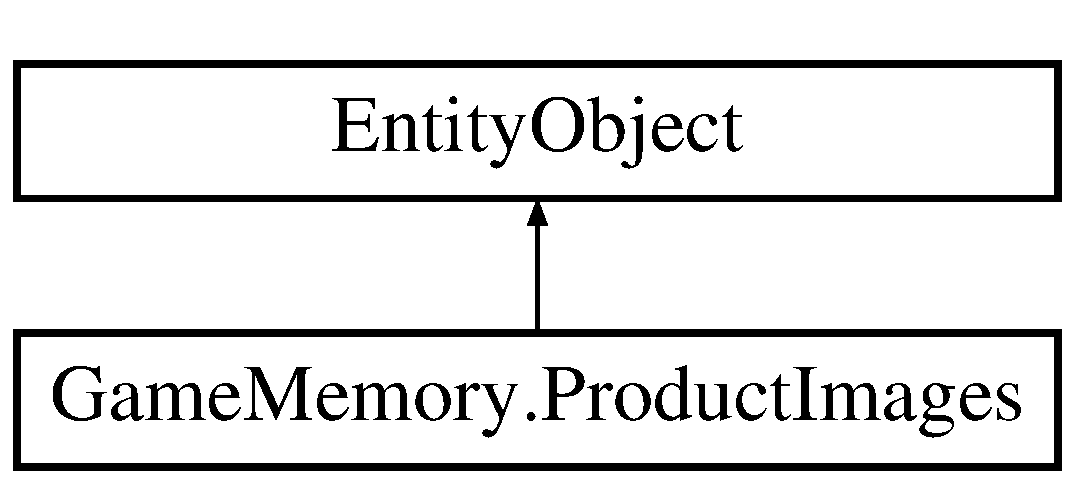
\includegraphics[height=2.000000cm]{class_game_memory_1_1_product_images}
\end{center}
\end{figure}
\subsection*{Static Public Member Functions}
\begin{DoxyCompactItemize}
\item 
static \hyperlink{class_game_memory_1_1_product_images}{Product\-Images} \hyperlink{class_game_memory_1_1_product_images_a28d6bdf672f7810dab416e5e3cd3dd86}{Create\-Product\-Images} (global\-::\-System.\-Int32 product\-Image\-Id)
\begin{DoxyCompactList}\small\item\em Crear un nuevo objeto \hyperlink{class_game_memory_1_1_product_images}{Product\-Images}. \end{DoxyCompactList}\end{DoxyCompactItemize}
\subsection*{Properties}
\begin{DoxyCompactItemize}
\item 
global\-::\-System.\-Int32 \hyperlink{class_game_memory_1_1_product_images_a8a6332671d553f887bcc162b3882550b}{Product\-Image\-Id}\hspace{0.3cm}{\ttfamily  \mbox{[}get, set\mbox{]}}
\begin{DoxyCompactList}\small\item\em No hay documentación de metadatos disponible. \end{DoxyCompactList}\item 
global\-::\-System.\-String \hyperlink{class_game_memory_1_1_product_images_aa11d5ca8f121efddb63bddd14530cfb9}{Caption}\hspace{0.3cm}{\ttfamily  \mbox{[}get, set\mbox{]}}
\begin{DoxyCompactList}\small\item\em No hay documentación de metadatos disponible. \end{DoxyCompactList}\item 
global\-::\-System.\-String \hyperlink{class_game_memory_1_1_product_images_a36f676489d4534cca829e8ee91b09619}{Title}\hspace{0.3cm}{\ttfamily  \mbox{[}get, set\mbox{]}}
\begin{DoxyCompactList}\small\item\em No hay documentación de metadatos disponible. \end{DoxyCompactList}\item 
global\-::\-System.\-String \hyperlink{class_game_memory_1_1_product_images_a09eaad03141a7a6aee9bee592a826fbb}{Size}\hspace{0.3cm}{\ttfamily  \mbox{[}get, set\mbox{]}}
\begin{DoxyCompactList}\small\item\em No hay documentación de metadatos disponible. \end{DoxyCompactList}\item 
global\-::\-System.\-String \hyperlink{class_game_memory_1_1_product_images_a3bb1f630d13a3acd2a74c75948ab7855}{Extension}\hspace{0.3cm}{\ttfamily  \mbox{[}get, set\mbox{]}}
\begin{DoxyCompactList}\small\item\em No hay documentación de metadatos disponible. \end{DoxyCompactList}\item 
Nullable$<$ global\-::\-System.\-Date\-Time $>$ \hyperlink{class_game_memory_1_1_product_images_a6e7dbbf06a198f98bdedd9d6a2f1522a}{Created\-Date}\hspace{0.3cm}{\ttfamily  \mbox{[}get, set\mbox{]}}
\begin{DoxyCompactList}\small\item\em No hay documentación de metadatos disponible. \end{DoxyCompactList}\item 
global\-::\-System.\-String \hyperlink{class_game_memory_1_1_product_images_aefd90f7ad4877c35455246a5960d3376}{Path}\hspace{0.3cm}{\ttfamily  \mbox{[}get, set\mbox{]}}
\begin{DoxyCompactList}\small\item\em No hay documentación de metadatos disponible. \end{DoxyCompactList}\item 
global\-::\-System.\-String \hyperlink{class_game_memory_1_1_product_images_a75804dbec1120967e319c7b68fa871c5}{Thumbnail\-Path}\hspace{0.3cm}{\ttfamily  \mbox{[}get, set\mbox{]}}
\begin{DoxyCompactList}\small\item\em No hay documentación de metadatos disponible. \end{DoxyCompactList}\item 
Entity\-Collection\\*
$<$ \hyperlink{class_game_memory_1_1_commercial_products}{Commercial\-Products} $>$ \hyperlink{class_game_memory_1_1_product_images_a24dde10ce929840666d5e7cfc9c2ecef}{Commercial\-Products}\hspace{0.3cm}{\ttfamily  \mbox{[}get, set\mbox{]}}
\begin{DoxyCompactList}\small\item\em No hay documentación de metadatos disponible. \end{DoxyCompactList}\end{DoxyCompactItemize}


\subsection{Detailed Description}
No hay documentación de metadatos disponible. 



\subsection{Member Function Documentation}
\hypertarget{class_game_memory_1_1_product_images_a28d6bdf672f7810dab416e5e3cd3dd86}{\index{Game\-Memory\-::\-Product\-Images@{Game\-Memory\-::\-Product\-Images}!Create\-Product\-Images@{Create\-Product\-Images}}
\index{Create\-Product\-Images@{Create\-Product\-Images}!GameMemory::ProductImages@{Game\-Memory\-::\-Product\-Images}}
\subsubsection[{Create\-Product\-Images}]{\setlength{\rightskip}{0pt plus 5cm}static {\bf Product\-Images} Game\-Memory.\-Product\-Images.\-Create\-Product\-Images (
\begin{DoxyParamCaption}
\item[{global\-::\-System.\-Int32}]{product\-Image\-Id}
\end{DoxyParamCaption}
)\hspace{0.3cm}{\ttfamily [static]}}}\label{class_game_memory_1_1_product_images_a28d6bdf672f7810dab416e5e3cd3dd86}


Crear un nuevo objeto \hyperlink{class_game_memory_1_1_product_images}{Product\-Images}. 


\begin{DoxyParams}{Parameters}
{\em product\-Image\-Id} & Valor inicial de la propiedad Product\-Image\-Id.\\
\hline
\end{DoxyParams}


\subsection{Property Documentation}
\hypertarget{class_game_memory_1_1_product_images_aa11d5ca8f121efddb63bddd14530cfb9}{\index{Game\-Memory\-::\-Product\-Images@{Game\-Memory\-::\-Product\-Images}!Caption@{Caption}}
\index{Caption@{Caption}!GameMemory::ProductImages@{Game\-Memory\-::\-Product\-Images}}
\subsubsection[{Caption}]{\setlength{\rightskip}{0pt plus 5cm}global.\-System.\-String Game\-Memory.\-Product\-Images.\-Caption\hspace{0.3cm}{\ttfamily [get]}, {\ttfamily [set]}}}\label{class_game_memory_1_1_product_images_aa11d5ca8f121efddb63bddd14530cfb9}


No hay documentación de metadatos disponible. 

\hypertarget{class_game_memory_1_1_product_images_a24dde10ce929840666d5e7cfc9c2ecef}{\index{Game\-Memory\-::\-Product\-Images@{Game\-Memory\-::\-Product\-Images}!Commercial\-Products@{Commercial\-Products}}
\index{Commercial\-Products@{Commercial\-Products}!GameMemory::ProductImages@{Game\-Memory\-::\-Product\-Images}}
\subsubsection[{Commercial\-Products}]{\setlength{\rightskip}{0pt plus 5cm}Entity\-Collection$<${\bf Commercial\-Products}$>$ Game\-Memory.\-Product\-Images.\-Commercial\-Products\hspace{0.3cm}{\ttfamily [get]}, {\ttfamily [set]}}}\label{class_game_memory_1_1_product_images_a24dde10ce929840666d5e7cfc9c2ecef}


No hay documentación de metadatos disponible. 

\hypertarget{class_game_memory_1_1_product_images_a6e7dbbf06a198f98bdedd9d6a2f1522a}{\index{Game\-Memory\-::\-Product\-Images@{Game\-Memory\-::\-Product\-Images}!Created\-Date@{Created\-Date}}
\index{Created\-Date@{Created\-Date}!GameMemory::ProductImages@{Game\-Memory\-::\-Product\-Images}}
\subsubsection[{Created\-Date}]{\setlength{\rightskip}{0pt plus 5cm}Nullable$<$global.\-System.\-Date\-Time$>$ Game\-Memory.\-Product\-Images.\-Created\-Date\hspace{0.3cm}{\ttfamily [get]}, {\ttfamily [set]}}}\label{class_game_memory_1_1_product_images_a6e7dbbf06a198f98bdedd9d6a2f1522a}


No hay documentación de metadatos disponible. 

\hypertarget{class_game_memory_1_1_product_images_a3bb1f630d13a3acd2a74c75948ab7855}{\index{Game\-Memory\-::\-Product\-Images@{Game\-Memory\-::\-Product\-Images}!Extension@{Extension}}
\index{Extension@{Extension}!GameMemory::ProductImages@{Game\-Memory\-::\-Product\-Images}}
\subsubsection[{Extension}]{\setlength{\rightskip}{0pt plus 5cm}global.\-System.\-String Game\-Memory.\-Product\-Images.\-Extension\hspace{0.3cm}{\ttfamily [get]}, {\ttfamily [set]}}}\label{class_game_memory_1_1_product_images_a3bb1f630d13a3acd2a74c75948ab7855}


No hay documentación de metadatos disponible. 

\hypertarget{class_game_memory_1_1_product_images_aefd90f7ad4877c35455246a5960d3376}{\index{Game\-Memory\-::\-Product\-Images@{Game\-Memory\-::\-Product\-Images}!Path@{Path}}
\index{Path@{Path}!GameMemory::ProductImages@{Game\-Memory\-::\-Product\-Images}}
\subsubsection[{Path}]{\setlength{\rightskip}{0pt plus 5cm}global.\-System.\-String Game\-Memory.\-Product\-Images.\-Path\hspace{0.3cm}{\ttfamily [get]}, {\ttfamily [set]}}}\label{class_game_memory_1_1_product_images_aefd90f7ad4877c35455246a5960d3376}


No hay documentación de metadatos disponible. 

\hypertarget{class_game_memory_1_1_product_images_a8a6332671d553f887bcc162b3882550b}{\index{Game\-Memory\-::\-Product\-Images@{Game\-Memory\-::\-Product\-Images}!Product\-Image\-Id@{Product\-Image\-Id}}
\index{Product\-Image\-Id@{Product\-Image\-Id}!GameMemory::ProductImages@{Game\-Memory\-::\-Product\-Images}}
\subsubsection[{Product\-Image\-Id}]{\setlength{\rightskip}{0pt plus 5cm}global.\-System.\-Int32 Game\-Memory.\-Product\-Images.\-Product\-Image\-Id\hspace{0.3cm}{\ttfamily [get]}, {\ttfamily [set]}}}\label{class_game_memory_1_1_product_images_a8a6332671d553f887bcc162b3882550b}


No hay documentación de metadatos disponible. 

\hypertarget{class_game_memory_1_1_product_images_a09eaad03141a7a6aee9bee592a826fbb}{\index{Game\-Memory\-::\-Product\-Images@{Game\-Memory\-::\-Product\-Images}!Size@{Size}}
\index{Size@{Size}!GameMemory::ProductImages@{Game\-Memory\-::\-Product\-Images}}
\subsubsection[{Size}]{\setlength{\rightskip}{0pt plus 5cm}global.\-System.\-String Game\-Memory.\-Product\-Images.\-Size\hspace{0.3cm}{\ttfamily [get]}, {\ttfamily [set]}}}\label{class_game_memory_1_1_product_images_a09eaad03141a7a6aee9bee592a826fbb}


No hay documentación de metadatos disponible. 

\hypertarget{class_game_memory_1_1_product_images_a75804dbec1120967e319c7b68fa871c5}{\index{Game\-Memory\-::\-Product\-Images@{Game\-Memory\-::\-Product\-Images}!Thumbnail\-Path@{Thumbnail\-Path}}
\index{Thumbnail\-Path@{Thumbnail\-Path}!GameMemory::ProductImages@{Game\-Memory\-::\-Product\-Images}}
\subsubsection[{Thumbnail\-Path}]{\setlength{\rightskip}{0pt plus 5cm}global.\-System.\-String Game\-Memory.\-Product\-Images.\-Thumbnail\-Path\hspace{0.3cm}{\ttfamily [get]}, {\ttfamily [set]}}}\label{class_game_memory_1_1_product_images_a75804dbec1120967e319c7b68fa871c5}


No hay documentación de metadatos disponible. 

\hypertarget{class_game_memory_1_1_product_images_a36f676489d4534cca829e8ee91b09619}{\index{Game\-Memory\-::\-Product\-Images@{Game\-Memory\-::\-Product\-Images}!Title@{Title}}
\index{Title@{Title}!GameMemory::ProductImages@{Game\-Memory\-::\-Product\-Images}}
\subsubsection[{Title}]{\setlength{\rightskip}{0pt plus 5cm}global.\-System.\-String Game\-Memory.\-Product\-Images.\-Title\hspace{0.3cm}{\ttfamily [get]}, {\ttfamily [set]}}}\label{class_game_memory_1_1_product_images_a36f676489d4534cca829e8ee91b09619}


No hay documentación de metadatos disponible. 



The documentation for this class was generated from the following file\-:\begin{DoxyCompactItemize}
\item 
D\-:/tesis\-Assembla/branches/\-Branch\-\_\-\-Tesis\-\_\-\-Sprint01/\-Dev/\-Interaction Module/\-Game\-Memory/\-Game\-Memory/O\-M\-K\-T.\-Designer.\-cs\end{DoxyCompactItemize}

\hypertarget{class_game_memory_1_1_roles}{\section{Game\-Memory.\-Roles Class Reference}
\label{class_game_memory_1_1_roles}\index{Game\-Memory.\-Roles@{Game\-Memory.\-Roles}}
}


No hay documentación de metadatos disponible.  


Inheritance diagram for Game\-Memory.\-Roles\-:\begin{figure}[H]
\begin{center}
\leavevmode
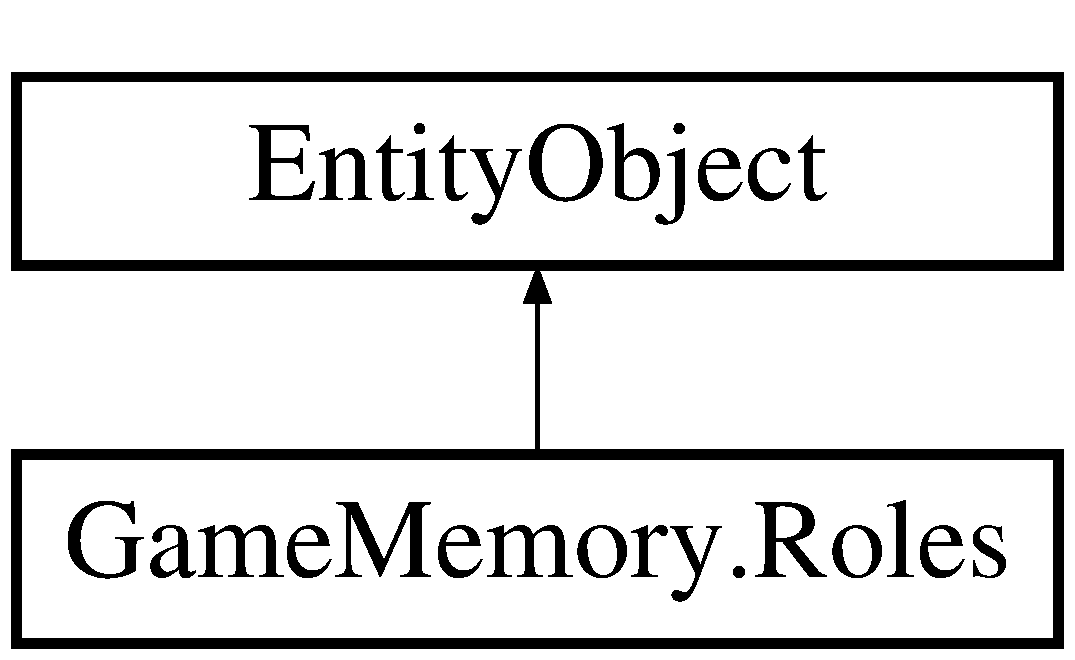
\includegraphics[height=2.000000cm]{class_game_memory_1_1_roles}
\end{center}
\end{figure}
\subsection*{Static Public Member Functions}
\begin{DoxyCompactItemize}
\item 
static \hyperlink{class_game_memory_1_1_roles}{Roles} \hyperlink{class_game_memory_1_1_roles_ae2ea4c860f98d4348a4d715b150ecbe5}{Create\-Roles} (global\-::\-System.\-Guid role\-Id, global\-::\-System.\-String role\-Name)
\begin{DoxyCompactList}\small\item\em Crear un nuevo objeto \hyperlink{class_game_memory_1_1_roles}{Roles}. \end{DoxyCompactList}\end{DoxyCompactItemize}
\subsection*{Properties}
\begin{DoxyCompactItemize}
\item 
global\-::\-System.\-Guid \hyperlink{class_game_memory_1_1_roles_a5bd242a9360210f533b781b88f8048e2}{Role\-Id}\hspace{0.3cm}{\ttfamily  \mbox{[}get, set\mbox{]}}
\begin{DoxyCompactList}\small\item\em No hay documentación de metadatos disponible. \end{DoxyCompactList}\item 
global\-::\-System.\-String \hyperlink{class_game_memory_1_1_roles_a0bb55986f20f2f4d2356cefc63638d16}{Role\-Name}\hspace{0.3cm}{\ttfamily  \mbox{[}get, set\mbox{]}}
\begin{DoxyCompactList}\small\item\em No hay documentación de metadatos disponible. \end{DoxyCompactList}\item 
global\-::\-System.\-String \hyperlink{class_game_memory_1_1_roles_a57a000be4763931423003c4d9a473567}{Description}\hspace{0.3cm}{\ttfamily  \mbox{[}get, set\mbox{]}}
\begin{DoxyCompactList}\small\item\em No hay documentación de metadatos disponible. \end{DoxyCompactList}\item 
Entity\-Collection$<$ \hyperlink{class_game_memory_1_1_users}{Users} $>$ \hyperlink{class_game_memory_1_1_roles_ad0095e11f320d6670960cfdf46f4c01c}{Users}\hspace{0.3cm}{\ttfamily  \mbox{[}get, set\mbox{]}}
\begin{DoxyCompactList}\small\item\em No hay documentación de metadatos disponible. \end{DoxyCompactList}\end{DoxyCompactItemize}


\subsection{Detailed Description}
No hay documentación de metadatos disponible. 



\subsection{Member Function Documentation}
\hypertarget{class_game_memory_1_1_roles_ae2ea4c860f98d4348a4d715b150ecbe5}{\index{Game\-Memory\-::\-Roles@{Game\-Memory\-::\-Roles}!Create\-Roles@{Create\-Roles}}
\index{Create\-Roles@{Create\-Roles}!GameMemory::Roles@{Game\-Memory\-::\-Roles}}
\subsubsection[{Create\-Roles}]{\setlength{\rightskip}{0pt plus 5cm}static {\bf Roles} Game\-Memory.\-Roles.\-Create\-Roles (
\begin{DoxyParamCaption}
\item[{global\-::\-System.\-Guid}]{role\-Id, }
\item[{global\-::\-System.\-String}]{role\-Name}
\end{DoxyParamCaption}
)\hspace{0.3cm}{\ttfamily [static]}}}\label{class_game_memory_1_1_roles_ae2ea4c860f98d4348a4d715b150ecbe5}


Crear un nuevo objeto \hyperlink{class_game_memory_1_1_roles}{Roles}. 


\begin{DoxyParams}{Parameters}
{\em role\-Id} & Valor inicial de la propiedad Role\-Id.\\
\hline
{\em role\-Name} & Valor inicial de la propiedad Role\-Name.\\
\hline
\end{DoxyParams}


\subsection{Property Documentation}
\hypertarget{class_game_memory_1_1_roles_a57a000be4763931423003c4d9a473567}{\index{Game\-Memory\-::\-Roles@{Game\-Memory\-::\-Roles}!Description@{Description}}
\index{Description@{Description}!GameMemory::Roles@{Game\-Memory\-::\-Roles}}
\subsubsection[{Description}]{\setlength{\rightskip}{0pt plus 5cm}global.\-System.\-String Game\-Memory.\-Roles.\-Description\hspace{0.3cm}{\ttfamily [get]}, {\ttfamily [set]}}}\label{class_game_memory_1_1_roles_a57a000be4763931423003c4d9a473567}


No hay documentación de metadatos disponible. 

\hypertarget{class_game_memory_1_1_roles_a5bd242a9360210f533b781b88f8048e2}{\index{Game\-Memory\-::\-Roles@{Game\-Memory\-::\-Roles}!Role\-Id@{Role\-Id}}
\index{Role\-Id@{Role\-Id}!GameMemory::Roles@{Game\-Memory\-::\-Roles}}
\subsubsection[{Role\-Id}]{\setlength{\rightskip}{0pt plus 5cm}global.\-System.\-Guid Game\-Memory.\-Roles.\-Role\-Id\hspace{0.3cm}{\ttfamily [get]}, {\ttfamily [set]}}}\label{class_game_memory_1_1_roles_a5bd242a9360210f533b781b88f8048e2}


No hay documentación de metadatos disponible. 

\hypertarget{class_game_memory_1_1_roles_a0bb55986f20f2f4d2356cefc63638d16}{\index{Game\-Memory\-::\-Roles@{Game\-Memory\-::\-Roles}!Role\-Name@{Role\-Name}}
\index{Role\-Name@{Role\-Name}!GameMemory::Roles@{Game\-Memory\-::\-Roles}}
\subsubsection[{Role\-Name}]{\setlength{\rightskip}{0pt plus 5cm}global.\-System.\-String Game\-Memory.\-Roles.\-Role\-Name\hspace{0.3cm}{\ttfamily [get]}, {\ttfamily [set]}}}\label{class_game_memory_1_1_roles_a0bb55986f20f2f4d2356cefc63638d16}


No hay documentación de metadatos disponible. 

\hypertarget{class_game_memory_1_1_roles_ad0095e11f320d6670960cfdf46f4c01c}{\index{Game\-Memory\-::\-Roles@{Game\-Memory\-::\-Roles}!Users@{Users}}
\index{Users@{Users}!GameMemory::Roles@{Game\-Memory\-::\-Roles}}
\subsubsection[{Users}]{\setlength{\rightskip}{0pt plus 5cm}Entity\-Collection$<${\bf Users}$>$ Game\-Memory.\-Roles.\-Users\hspace{0.3cm}{\ttfamily [get]}, {\ttfamily [set]}}}\label{class_game_memory_1_1_roles_ad0095e11f320d6670960cfdf46f4c01c}


No hay documentación de metadatos disponible. 



The documentation for this class was generated from the following file\-:\begin{DoxyCompactItemize}
\item 
D\-:/tesis\-Assembla/branches/\-Branch\-\_\-\-Tesis\-\_\-\-Sprint01/\-Dev/\-Interaction Module/\-Game\-Memory/\-Game\-Memory/O\-M\-K\-T.\-Designer.\-cs\end{DoxyCompactItemize}

\hypertarget{class_game_memory_1_1_snapshots}{\section{Game\-Memory.\-Snapshots Class Reference}
\label{class_game_memory_1_1_snapshots}\index{Game\-Memory.\-Snapshots@{Game\-Memory.\-Snapshots}}
}


No hay documentación de metadatos disponible.  


Inheritance diagram for Game\-Memory.\-Snapshots\-:\begin{figure}[H]
\begin{center}
\leavevmode
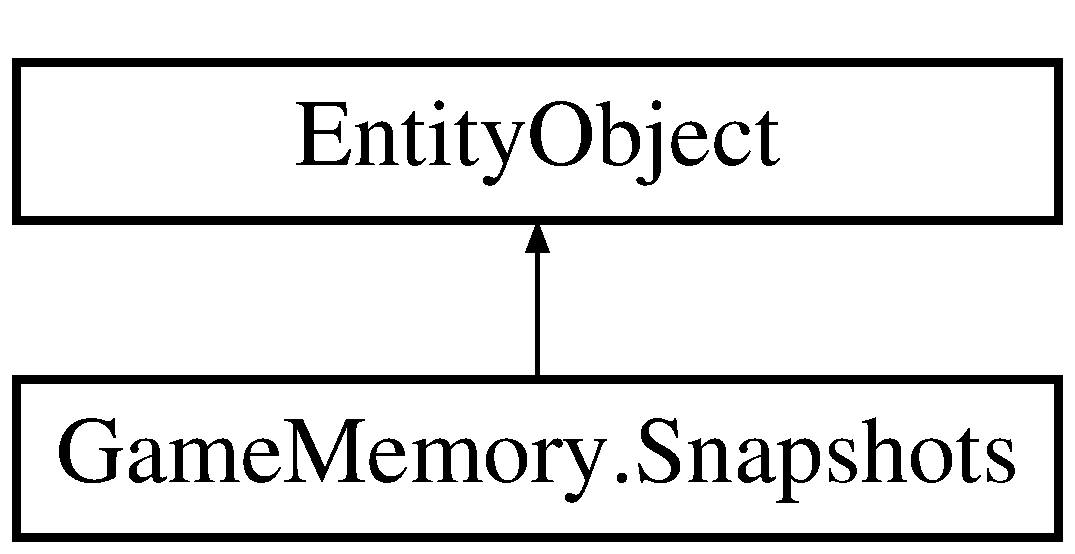
\includegraphics[height=2.000000cm]{class_game_memory_1_1_snapshots}
\end{center}
\end{figure}
\subsection*{Static Public Member Functions}
\begin{DoxyCompactItemize}
\item 
static \hyperlink{class_game_memory_1_1_snapshots}{Snapshots} \hyperlink{class_game_memory_1_1_snapshots_a4d7ce7690220df76d6140fc067e0adb4}{Create\-Snapshots} (global\-::\-System.\-Int32 snapshot\-Id, global\-::\-System.\-Int32 quantity)
\begin{DoxyCompactList}\small\item\em Crear un nuevo objeto \hyperlink{class_game_memory_1_1_snapshots}{Snapshots}. \end{DoxyCompactList}\end{DoxyCompactItemize}
\subsection*{Properties}
\begin{DoxyCompactItemize}
\item 
global\-::\-System.\-Int32 \hyperlink{class_game_memory_1_1_snapshots_ae7206905beee36fb1e969c02a263aa0f}{Snapshot\-Id}\hspace{0.3cm}{\ttfamily  \mbox{[}get, set\mbox{]}}
\begin{DoxyCompactList}\small\item\em No hay documentación de metadatos disponible. \end{DoxyCompactList}\item 
global\-::\-System.\-Int32 \hyperlink{class_game_memory_1_1_snapshots_ac4c2dd5b199a89212283b3ea085db5c9}{Quantity}\hspace{0.3cm}{\ttfamily  \mbox{[}get, set\mbox{]}}
\begin{DoxyCompactList}\small\item\em No hay documentación de metadatos disponible. \end{DoxyCompactList}\item 
global\-::\-System.\-String \hyperlink{class_game_memory_1_1_snapshots_abb210bf16aaff23bec1a023f5fcbd2f3}{Path}\hspace{0.3cm}{\ttfamily  \mbox{[}get, set\mbox{]}}
\begin{DoxyCompactList}\small\item\em No hay documentación de metadatos disponible. \end{DoxyCompactList}\item 
Entity\-Collection$<$ \hyperlink{class_game_memory_1_1_interactions}{Interactions} $>$ \hyperlink{class_game_memory_1_1_snapshots_a24c7654eba40312f235c515e732088dc}{Interactions}\hspace{0.3cm}{\ttfamily  \mbox{[}get, set\mbox{]}}
\begin{DoxyCompactList}\small\item\em No hay documentación de metadatos disponible. \end{DoxyCompactList}\end{DoxyCompactItemize}


\subsection{Detailed Description}
No hay documentación de metadatos disponible. 



\subsection{Member Function Documentation}
\hypertarget{class_game_memory_1_1_snapshots_a4d7ce7690220df76d6140fc067e0adb4}{\index{Game\-Memory\-::\-Snapshots@{Game\-Memory\-::\-Snapshots}!Create\-Snapshots@{Create\-Snapshots}}
\index{Create\-Snapshots@{Create\-Snapshots}!GameMemory::Snapshots@{Game\-Memory\-::\-Snapshots}}
\subsubsection[{Create\-Snapshots}]{\setlength{\rightskip}{0pt plus 5cm}static {\bf Snapshots} Game\-Memory.\-Snapshots.\-Create\-Snapshots (
\begin{DoxyParamCaption}
\item[{global\-::\-System.\-Int32}]{snapshot\-Id, }
\item[{global\-::\-System.\-Int32}]{quantity}
\end{DoxyParamCaption}
)\hspace{0.3cm}{\ttfamily [static]}}}\label{class_game_memory_1_1_snapshots_a4d7ce7690220df76d6140fc067e0adb4}


Crear un nuevo objeto \hyperlink{class_game_memory_1_1_snapshots}{Snapshots}. 


\begin{DoxyParams}{Parameters}
{\em snapshot\-Id} & Valor inicial de la propiedad Snapshot\-Id.\\
\hline
{\em quantity} & Valor inicial de la propiedad Quantity.\\
\hline
\end{DoxyParams}


\subsection{Property Documentation}
\hypertarget{class_game_memory_1_1_snapshots_a24c7654eba40312f235c515e732088dc}{\index{Game\-Memory\-::\-Snapshots@{Game\-Memory\-::\-Snapshots}!Interactions@{Interactions}}
\index{Interactions@{Interactions}!GameMemory::Snapshots@{Game\-Memory\-::\-Snapshots}}
\subsubsection[{Interactions}]{\setlength{\rightskip}{0pt plus 5cm}Entity\-Collection$<${\bf Interactions}$>$ Game\-Memory.\-Snapshots.\-Interactions\hspace{0.3cm}{\ttfamily [get]}, {\ttfamily [set]}}}\label{class_game_memory_1_1_snapshots_a24c7654eba40312f235c515e732088dc}


No hay documentación de metadatos disponible. 

\hypertarget{class_game_memory_1_1_snapshots_abb210bf16aaff23bec1a023f5fcbd2f3}{\index{Game\-Memory\-::\-Snapshots@{Game\-Memory\-::\-Snapshots}!Path@{Path}}
\index{Path@{Path}!GameMemory::Snapshots@{Game\-Memory\-::\-Snapshots}}
\subsubsection[{Path}]{\setlength{\rightskip}{0pt plus 5cm}global.\-System.\-String Game\-Memory.\-Snapshots.\-Path\hspace{0.3cm}{\ttfamily [get]}, {\ttfamily [set]}}}\label{class_game_memory_1_1_snapshots_abb210bf16aaff23bec1a023f5fcbd2f3}


No hay documentación de metadatos disponible. 

\hypertarget{class_game_memory_1_1_snapshots_ac4c2dd5b199a89212283b3ea085db5c9}{\index{Game\-Memory\-::\-Snapshots@{Game\-Memory\-::\-Snapshots}!Quantity@{Quantity}}
\index{Quantity@{Quantity}!GameMemory::Snapshots@{Game\-Memory\-::\-Snapshots}}
\subsubsection[{Quantity}]{\setlength{\rightskip}{0pt plus 5cm}global.\-System.\-Int32 Game\-Memory.\-Snapshots.\-Quantity\hspace{0.3cm}{\ttfamily [get]}, {\ttfamily [set]}}}\label{class_game_memory_1_1_snapshots_ac4c2dd5b199a89212283b3ea085db5c9}


No hay documentación de metadatos disponible. 

\hypertarget{class_game_memory_1_1_snapshots_ae7206905beee36fb1e969c02a263aa0f}{\index{Game\-Memory\-::\-Snapshots@{Game\-Memory\-::\-Snapshots}!Snapshot\-Id@{Snapshot\-Id}}
\index{Snapshot\-Id@{Snapshot\-Id}!GameMemory::Snapshots@{Game\-Memory\-::\-Snapshots}}
\subsubsection[{Snapshot\-Id}]{\setlength{\rightskip}{0pt plus 5cm}global.\-System.\-Int32 Game\-Memory.\-Snapshots.\-Snapshot\-Id\hspace{0.3cm}{\ttfamily [get]}, {\ttfamily [set]}}}\label{class_game_memory_1_1_snapshots_ae7206905beee36fb1e969c02a263aa0f}


No hay documentación de metadatos disponible. 



The documentation for this class was generated from the following file\-:\begin{DoxyCompactItemize}
\item 
D\-:/tesis\-Assembla/branches/\-Branch\-\_\-\-Tesis\-\_\-\-Sprint01/\-Dev/\-Interaction Module/\-Game\-Memory/\-Game\-Memory/O\-M\-K\-T.\-Designer.\-cs\end{DoxyCompactItemize}

\hypertarget{class_game_memory_1_1_sort_types}{\section{Game\-Memory.\-Sort\-Types Class Reference}
\label{class_game_memory_1_1_sort_types}\index{Game\-Memory.\-Sort\-Types@{Game\-Memory.\-Sort\-Types}}
}


No hay documentación de metadatos disponible.  


Inheritance diagram for Game\-Memory.\-Sort\-Types\-:\begin{figure}[H]
\begin{center}
\leavevmode
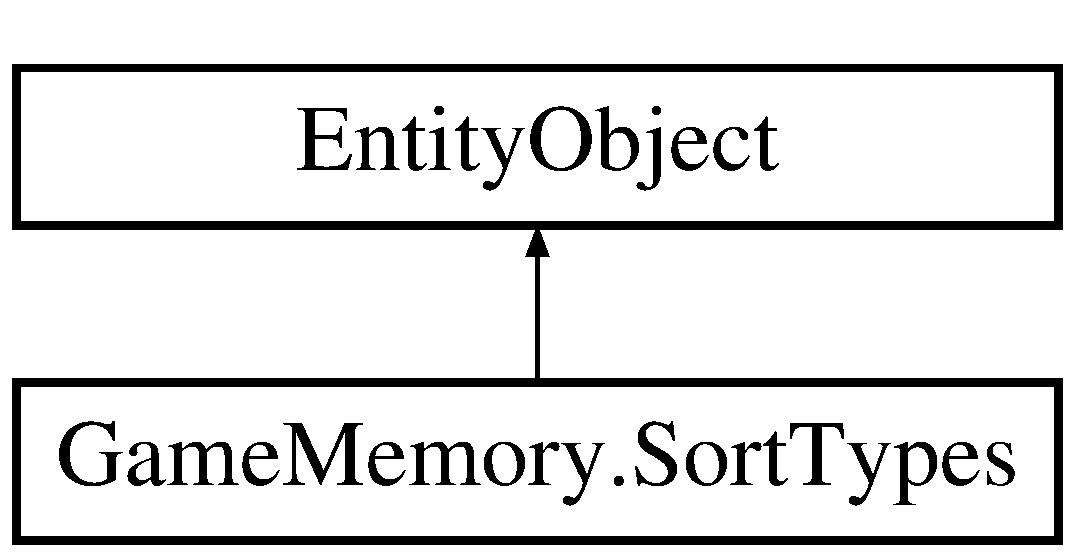
\includegraphics[height=2.000000cm]{class_game_memory_1_1_sort_types}
\end{center}
\end{figure}
\subsection*{Static Public Member Functions}
\begin{DoxyCompactItemize}
\item 
static \hyperlink{class_game_memory_1_1_sort_types}{Sort\-Types} \hyperlink{class_game_memory_1_1_sort_types_ab951bab06c0cc7f65eff26dcef0585ff}{Create\-Sort\-Types} (global\-::\-System.\-Int32 sort\-Type\-Id)
\begin{DoxyCompactList}\small\item\em Crear un nuevo objeto \hyperlink{class_game_memory_1_1_sort_types}{Sort\-Types}. \end{DoxyCompactList}\end{DoxyCompactItemize}
\subsection*{Properties}
\begin{DoxyCompactItemize}
\item 
global\-::\-System.\-Int32 \hyperlink{class_game_memory_1_1_sort_types_a49fac50b119c2c0286cfdbd9769dea4a}{Sort\-Type\-Id}\hspace{0.3cm}{\ttfamily  \mbox{[}get, set\mbox{]}}
\begin{DoxyCompactList}\small\item\em No hay documentación de metadatos disponible. \end{DoxyCompactList}\item 
global\-::\-System.\-String \hyperlink{class_game_memory_1_1_sort_types_a41a4b183e89b71b60a52e58fba2d3c6f}{Name}\hspace{0.3cm}{\ttfamily  \mbox{[}get, set\mbox{]}}
\begin{DoxyCompactList}\small\item\em No hay documentación de metadatos disponible. \end{DoxyCompactList}\item 
global\-::\-System.\-String \hyperlink{class_game_memory_1_1_sort_types_a1b9776a951d3683388021e927ca1a5fb}{Description}\hspace{0.3cm}{\ttfamily  \mbox{[}get, set\mbox{]}}
\begin{DoxyCompactList}\small\item\em No hay documentación de metadatos disponible. \end{DoxyCompactList}\item 
Entity\-Collection$<$ \hyperlink{class_game_memory_1_1_adverts}{Adverts} $>$ \hyperlink{class_game_memory_1_1_sort_types_ab9ce3a68aab30a9339f7a9fde700ce25}{Adverts}\hspace{0.3cm}{\ttfamily  \mbox{[}get, set\mbox{]}}
\begin{DoxyCompactList}\small\item\em No hay documentación de metadatos disponible. \end{DoxyCompactList}\end{DoxyCompactItemize}


\subsection{Detailed Description}
No hay documentación de metadatos disponible. 



\subsection{Member Function Documentation}
\hypertarget{class_game_memory_1_1_sort_types_ab951bab06c0cc7f65eff26dcef0585ff}{\index{Game\-Memory\-::\-Sort\-Types@{Game\-Memory\-::\-Sort\-Types}!Create\-Sort\-Types@{Create\-Sort\-Types}}
\index{Create\-Sort\-Types@{Create\-Sort\-Types}!GameMemory::SortTypes@{Game\-Memory\-::\-Sort\-Types}}
\subsubsection[{Create\-Sort\-Types}]{\setlength{\rightskip}{0pt plus 5cm}static {\bf Sort\-Types} Game\-Memory.\-Sort\-Types.\-Create\-Sort\-Types (
\begin{DoxyParamCaption}
\item[{global\-::\-System.\-Int32}]{sort\-Type\-Id}
\end{DoxyParamCaption}
)\hspace{0.3cm}{\ttfamily [static]}}}\label{class_game_memory_1_1_sort_types_ab951bab06c0cc7f65eff26dcef0585ff}


Crear un nuevo objeto \hyperlink{class_game_memory_1_1_sort_types}{Sort\-Types}. 


\begin{DoxyParams}{Parameters}
{\em sort\-Type\-Id} & Valor inicial de la propiedad Sort\-Type\-Id.\\
\hline
\end{DoxyParams}


\subsection{Property Documentation}
\hypertarget{class_game_memory_1_1_sort_types_ab9ce3a68aab30a9339f7a9fde700ce25}{\index{Game\-Memory\-::\-Sort\-Types@{Game\-Memory\-::\-Sort\-Types}!Adverts@{Adverts}}
\index{Adverts@{Adverts}!GameMemory::SortTypes@{Game\-Memory\-::\-Sort\-Types}}
\subsubsection[{Adverts}]{\setlength{\rightskip}{0pt plus 5cm}Entity\-Collection$<${\bf Adverts}$>$ Game\-Memory.\-Sort\-Types.\-Adverts\hspace{0.3cm}{\ttfamily [get]}, {\ttfamily [set]}}}\label{class_game_memory_1_1_sort_types_ab9ce3a68aab30a9339f7a9fde700ce25}


No hay documentación de metadatos disponible. 

\hypertarget{class_game_memory_1_1_sort_types_a1b9776a951d3683388021e927ca1a5fb}{\index{Game\-Memory\-::\-Sort\-Types@{Game\-Memory\-::\-Sort\-Types}!Description@{Description}}
\index{Description@{Description}!GameMemory::SortTypes@{Game\-Memory\-::\-Sort\-Types}}
\subsubsection[{Description}]{\setlength{\rightskip}{0pt plus 5cm}global.\-System.\-String Game\-Memory.\-Sort\-Types.\-Description\hspace{0.3cm}{\ttfamily [get]}, {\ttfamily [set]}}}\label{class_game_memory_1_1_sort_types_a1b9776a951d3683388021e927ca1a5fb}


No hay documentación de metadatos disponible. 

\hypertarget{class_game_memory_1_1_sort_types_a41a4b183e89b71b60a52e58fba2d3c6f}{\index{Game\-Memory\-::\-Sort\-Types@{Game\-Memory\-::\-Sort\-Types}!Name@{Name}}
\index{Name@{Name}!GameMemory::SortTypes@{Game\-Memory\-::\-Sort\-Types}}
\subsubsection[{Name}]{\setlength{\rightskip}{0pt plus 5cm}global.\-System.\-String Game\-Memory.\-Sort\-Types.\-Name\hspace{0.3cm}{\ttfamily [get]}, {\ttfamily [set]}}}\label{class_game_memory_1_1_sort_types_a41a4b183e89b71b60a52e58fba2d3c6f}


No hay documentación de metadatos disponible. 

\hypertarget{class_game_memory_1_1_sort_types_a49fac50b119c2c0286cfdbd9769dea4a}{\index{Game\-Memory\-::\-Sort\-Types@{Game\-Memory\-::\-Sort\-Types}!Sort\-Type\-Id@{Sort\-Type\-Id}}
\index{Sort\-Type\-Id@{Sort\-Type\-Id}!GameMemory::SortTypes@{Game\-Memory\-::\-Sort\-Types}}
\subsubsection[{Sort\-Type\-Id}]{\setlength{\rightskip}{0pt plus 5cm}global.\-System.\-Int32 Game\-Memory.\-Sort\-Types.\-Sort\-Type\-Id\hspace{0.3cm}{\ttfamily [get]}, {\ttfamily [set]}}}\label{class_game_memory_1_1_sort_types_a49fac50b119c2c0286cfdbd9769dea4a}


No hay documentación de metadatos disponible. 



The documentation for this class was generated from the following file\-:\begin{DoxyCompactItemize}
\item 
D\-:/tesis\-Assembla/branches/\-Branch\-\_\-\-Tesis\-\_\-\-Sprint01/\-Dev/\-Interaction Module/\-Game\-Memory/\-Game\-Memory/O\-M\-K\-T.\-Designer.\-cs\end{DoxyCompactItemize}

\hypertarget{class_game_memory_1_1_users}{\section{Game\-Memory.\-Users Class Reference}
\label{class_game_memory_1_1_users}\index{Game\-Memory.\-Users@{Game\-Memory.\-Users}}
}


No hay documentación de metadatos disponible.  


Inheritance diagram for Game\-Memory.\-Users\-:\begin{figure}[H]
\begin{center}
\leavevmode
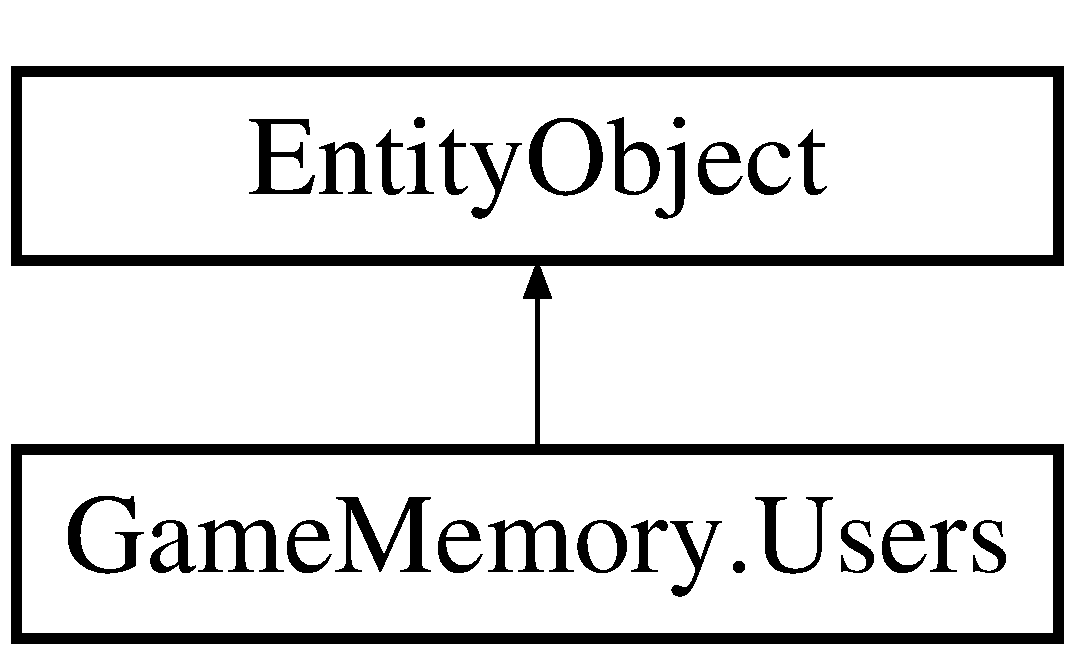
\includegraphics[height=2.000000cm]{class_game_memory_1_1_users}
\end{center}
\end{figure}
\subsection*{Static Public Member Functions}
\begin{DoxyCompactItemize}
\item 
static \hyperlink{class_game_memory_1_1_users}{Users} \hyperlink{class_game_memory_1_1_users_a299cec11198e4aaa738c60c535dd3af4}{Create\-Users} (global\-::\-System.\-Guid user\-Id, global\-::\-System.\-String username, global\-::\-System.\-String email, global\-::\-System.\-String password, global\-::\-System.\-Boolean is\-Approved, global\-::\-System.\-Int32 password\-Failures\-Since\-Last\-Success, global\-::\-System.\-Boolean is\-Locked\-Out, global\-::\-System.\-Int32 customer\-Id)
\begin{DoxyCompactList}\small\item\em Crear un nuevo objeto \hyperlink{class_game_memory_1_1_users}{Users}. \end{DoxyCompactList}\end{DoxyCompactItemize}
\subsection*{Properties}
\begin{DoxyCompactItemize}
\item 
global\-::\-System.\-Guid \hyperlink{class_game_memory_1_1_users_a719eefec747bdad64f34d721febf4aef}{User\-Id}\hspace{0.3cm}{\ttfamily  \mbox{[}get, set\mbox{]}}
\begin{DoxyCompactList}\small\item\em No hay documentación de metadatos disponible. \end{DoxyCompactList}\item 
global\-::\-System.\-String \hyperlink{class_game_memory_1_1_users_a679995b1dfe9cb52a344232e32351a57}{Username}\hspace{0.3cm}{\ttfamily  \mbox{[}get, set\mbox{]}}
\begin{DoxyCompactList}\small\item\em No hay documentación de metadatos disponible. \end{DoxyCompactList}\item 
global\-::\-System.\-String \hyperlink{class_game_memory_1_1_users_aae427c5afcfec36bc3e06a306b631ca3}{Email}\hspace{0.3cm}{\ttfamily  \mbox{[}get, set\mbox{]}}
\begin{DoxyCompactList}\small\item\em No hay documentación de metadatos disponible. \end{DoxyCompactList}\item 
global\-::\-System.\-String \hyperlink{class_game_memory_1_1_users_abb226cc2dac045639deb3f1efa109fab}{Password}\hspace{0.3cm}{\ttfamily  \mbox{[}get, set\mbox{]}}
\begin{DoxyCompactList}\small\item\em No hay documentación de metadatos disponible. \end{DoxyCompactList}\item 
global\-::\-System.\-String \hyperlink{class_game_memory_1_1_users_af6e34812d5ef60563a0566e65bbe5e6b}{First\-Name}\hspace{0.3cm}{\ttfamily  \mbox{[}get, set\mbox{]}}
\begin{DoxyCompactList}\small\item\em No hay documentación de metadatos disponible. \end{DoxyCompactList}\item 
global\-::\-System.\-String \hyperlink{class_game_memory_1_1_users_a440ecd49516fc34c62e82845bcefbb69}{Last\-Name}\hspace{0.3cm}{\ttfamily  \mbox{[}get, set\mbox{]}}
\begin{DoxyCompactList}\small\item\em No hay documentación de metadatos disponible. \end{DoxyCompactList}\item 
global\-::\-System.\-String \hyperlink{class_game_memory_1_1_users_a78fc5aef90521ab4a0d0ffa82eb5a27a}{Comment}\hspace{0.3cm}{\ttfamily  \mbox{[}get, set\mbox{]}}
\begin{DoxyCompactList}\small\item\em No hay documentación de metadatos disponible. \end{DoxyCompactList}\item 
global\-::\-System.\-Boolean \hyperlink{class_game_memory_1_1_users_a112ee494edcaeda109a5ea967b60273c}{Is\-Approved}\hspace{0.3cm}{\ttfamily  \mbox{[}get, set\mbox{]}}
\begin{DoxyCompactList}\small\item\em No hay documentación de metadatos disponible. \end{DoxyCompactList}\item 
global\-::\-System.\-Int32 \hyperlink{class_game_memory_1_1_users_a58dec1e298fb45ba5d9110a151260392}{Password\-Failures\-Since\-Last\-Success}\hspace{0.3cm}{\ttfamily  \mbox{[}get, set\mbox{]}}
\begin{DoxyCompactList}\small\item\em No hay documentación de metadatos disponible. \end{DoxyCompactList}\item 
Nullable$<$ global\-::\-System.\-Date\-Time $>$ \hyperlink{class_game_memory_1_1_users_a0383048727d3c375e860db6310087196}{Last\-Password\-Failure\-Date}\hspace{0.3cm}{\ttfamily  \mbox{[}get, set\mbox{]}}
\begin{DoxyCompactList}\small\item\em No hay documentación de metadatos disponible. \end{DoxyCompactList}\item 
Nullable$<$ global\-::\-System.\-Date\-Time $>$ \hyperlink{class_game_memory_1_1_users_a86ea14d379459264427b6109be5a1a59}{Last\-Activity\-Date}\hspace{0.3cm}{\ttfamily  \mbox{[}get, set\mbox{]}}
\begin{DoxyCompactList}\small\item\em No hay documentación de metadatos disponible. \end{DoxyCompactList}\item 
Nullable$<$ global\-::\-System.\-Date\-Time $>$ \hyperlink{class_game_memory_1_1_users_aac14661b4cd2906d5d4699b9b1b6fea8}{Last\-Lockout\-Date}\hspace{0.3cm}{\ttfamily  \mbox{[}get, set\mbox{]}}
\begin{DoxyCompactList}\small\item\em No hay documentación de metadatos disponible. \end{DoxyCompactList}\item 
Nullable$<$ global\-::\-System.\-Date\-Time $>$ \hyperlink{class_game_memory_1_1_users_a7c3fd7829e1bcff44f1ddf93163c7a7e}{Date\-Of\-Birth}\hspace{0.3cm}{\ttfamily  \mbox{[}get, set\mbox{]}}
\begin{DoxyCompactList}\small\item\em No hay documentación de metadatos disponible. \end{DoxyCompactList}\item 
Nullable$<$ global\-::\-System.\-Date\-Time $>$ \hyperlink{class_game_memory_1_1_users_abb9ebf3a6108d29f1eea6eec2142b3d1}{Last\-Login\-Date}\hspace{0.3cm}{\ttfamily  \mbox{[}get, set\mbox{]}}
\begin{DoxyCompactList}\small\item\em No hay documentación de metadatos disponible. \end{DoxyCompactList}\item 
global\-::\-System.\-String \hyperlink{class_game_memory_1_1_users_aae1d5f9c95e32efb79d2d1a5ec2e76f9}{Confirmation\-Token}\hspace{0.3cm}{\ttfamily  \mbox{[}get, set\mbox{]}}
\begin{DoxyCompactList}\small\item\em No hay documentación de metadatos disponible. \end{DoxyCompactList}\item 
Nullable$<$ global\-::\-System.\-Date\-Time $>$ \hyperlink{class_game_memory_1_1_users_ad285931a74d022fafbd9299b88e2125a}{Create\-Date}\hspace{0.3cm}{\ttfamily  \mbox{[}get, set\mbox{]}}
\begin{DoxyCompactList}\small\item\em No hay documentación de metadatos disponible. \end{DoxyCompactList}\item 
global\-::\-System.\-Boolean \hyperlink{class_game_memory_1_1_users_a4def29e0222bfd127b6859ade7a5ca87}{Is\-Locked\-Out}\hspace{0.3cm}{\ttfamily  \mbox{[}get, set\mbox{]}}
\begin{DoxyCompactList}\small\item\em No hay documentación de metadatos disponible. \end{DoxyCompactList}\item 
Nullable$<$ global\-::\-System.\-Date\-Time $>$ \hyperlink{class_game_memory_1_1_users_a98f39140ef43f86f9edcff50e40c982a}{Last\-Password\-Changed\-Date}\hspace{0.3cm}{\ttfamily  \mbox{[}get, set\mbox{]}}
\begin{DoxyCompactList}\small\item\em No hay documentación de metadatos disponible. \end{DoxyCompactList}\item 
global\-::\-System.\-String \hyperlink{class_game_memory_1_1_users_a70980afbd2f715e7238fc3e8ffcb4741}{Password\-Verification\-Token}\hspace{0.3cm}{\ttfamily  \mbox{[}get, set\mbox{]}}
\begin{DoxyCompactList}\small\item\em No hay documentación de metadatos disponible. \end{DoxyCompactList}\item 
Nullable$<$ global\-::\-System.\-Date\-Time $>$ \hyperlink{class_game_memory_1_1_users_af5736cddf03b326304374ae1352404d1}{Password\-Verification\-Token\-Expiration\-Date}\hspace{0.3cm}{\ttfamily  \mbox{[}get, set\mbox{]}}
\begin{DoxyCompactList}\small\item\em No hay documentación de metadatos disponible. \end{DoxyCompactList}\item 
global\-::\-System.\-Int32 \hyperlink{class_game_memory_1_1_users_a7374f9d0dc506d2044098f621fd5397a}{Customer\-Id}\hspace{0.3cm}{\ttfamily  \mbox{[}get, set\mbox{]}}
\begin{DoxyCompactList}\small\item\em No hay documentación de metadatos disponible. \end{DoxyCompactList}\item 
\hyperlink{class_game_memory_1_1_customers}{Customers} \hyperlink{class_game_memory_1_1_users_aa00fe3516ae95f465ff77d338217736a}{Customers}\hspace{0.3cm}{\ttfamily  \mbox{[}get, set\mbox{]}}
\begin{DoxyCompactList}\small\item\em No hay documentación de metadatos disponible. \end{DoxyCompactList}\item 
Entity\-Reference$<$ \hyperlink{class_game_memory_1_1_customers}{Customers} $>$ \hyperlink{class_game_memory_1_1_users_ade92ef696dff98620ce322dedfcd7b52}{Customers\-Reference}\hspace{0.3cm}{\ttfamily  \mbox{[}get, set\mbox{]}}
\begin{DoxyCompactList}\small\item\em No hay documentación de metadatos disponible. \end{DoxyCompactList}\item 
Entity\-Collection$<$ \hyperlink{class_game_memory_1_1_inboxes}{Inboxes} $>$ \hyperlink{class_game_memory_1_1_users_a612925fd6d50f8624a9067e930bcbe37}{Inboxes}\hspace{0.3cm}{\ttfamily  \mbox{[}get, set\mbox{]}}
\begin{DoxyCompactList}\small\item\em No hay documentación de metadatos disponible. \end{DoxyCompactList}\item 
Entity\-Collection$<$ \hyperlink{class_game_memory_1_1_roles}{Roles} $>$ \hyperlink{class_game_memory_1_1_users_a1dea6fa0cc9c30a97d4090a9523a1d72}{Roles}\hspace{0.3cm}{\ttfamily  \mbox{[}get, set\mbox{]}}
\begin{DoxyCompactList}\small\item\em No hay documentación de metadatos disponible. \end{DoxyCompactList}\end{DoxyCompactItemize}


\subsection{Detailed Description}
No hay documentación de metadatos disponible. 



\subsection{Member Function Documentation}
\hypertarget{class_game_memory_1_1_users_a299cec11198e4aaa738c60c535dd3af4}{\index{Game\-Memory\-::\-Users@{Game\-Memory\-::\-Users}!Create\-Users@{Create\-Users}}
\index{Create\-Users@{Create\-Users}!GameMemory::Users@{Game\-Memory\-::\-Users}}
\subsubsection[{Create\-Users}]{\setlength{\rightskip}{0pt plus 5cm}static {\bf Users} Game\-Memory.\-Users.\-Create\-Users (
\begin{DoxyParamCaption}
\item[{global\-::\-System.\-Guid}]{user\-Id, }
\item[{global\-::\-System.\-String}]{username, }
\item[{global\-::\-System.\-String}]{email, }
\item[{global\-::\-System.\-String}]{password, }
\item[{global\-::\-System.\-Boolean}]{is\-Approved, }
\item[{global\-::\-System.\-Int32}]{password\-Failures\-Since\-Last\-Success, }
\item[{global\-::\-System.\-Boolean}]{is\-Locked\-Out, }
\item[{global\-::\-System.\-Int32}]{customer\-Id}
\end{DoxyParamCaption}
)\hspace{0.3cm}{\ttfamily [static]}}}\label{class_game_memory_1_1_users_a299cec11198e4aaa738c60c535dd3af4}


Crear un nuevo objeto \hyperlink{class_game_memory_1_1_users}{Users}. 


\begin{DoxyParams}{Parameters}
{\em user\-Id} & Valor inicial de la propiedad User\-Id.\\
\hline
{\em username} & Valor inicial de la propiedad Username.\\
\hline
{\em email} & Valor inicial de la propiedad Email.\\
\hline
{\em password} & Valor inicial de la propiedad Password.\\
\hline
{\em is\-Approved} & Valor inicial de la propiedad Is\-Approved.\\
\hline
{\em password\-Failures\-Since\-Last\-Success} & Valor inicial de la propiedad Password\-Failures\-Since\-Last\-Success.\\
\hline
{\em is\-Locked\-Out} & Valor inicial de la propiedad Is\-Locked\-Out.\\
\hline
{\em customer\-Id} & Valor inicial de la propiedad Customer\-Id.\\
\hline
\end{DoxyParams}


\subsection{Property Documentation}
\hypertarget{class_game_memory_1_1_users_a78fc5aef90521ab4a0d0ffa82eb5a27a}{\index{Game\-Memory\-::\-Users@{Game\-Memory\-::\-Users}!Comment@{Comment}}
\index{Comment@{Comment}!GameMemory::Users@{Game\-Memory\-::\-Users}}
\subsubsection[{Comment}]{\setlength{\rightskip}{0pt plus 5cm}global.\-System.\-String Game\-Memory.\-Users.\-Comment\hspace{0.3cm}{\ttfamily [get]}, {\ttfamily [set]}}}\label{class_game_memory_1_1_users_a78fc5aef90521ab4a0d0ffa82eb5a27a}


No hay documentación de metadatos disponible. 

\hypertarget{class_game_memory_1_1_users_aae1d5f9c95e32efb79d2d1a5ec2e76f9}{\index{Game\-Memory\-::\-Users@{Game\-Memory\-::\-Users}!Confirmation\-Token@{Confirmation\-Token}}
\index{Confirmation\-Token@{Confirmation\-Token}!GameMemory::Users@{Game\-Memory\-::\-Users}}
\subsubsection[{Confirmation\-Token}]{\setlength{\rightskip}{0pt plus 5cm}global.\-System.\-String Game\-Memory.\-Users.\-Confirmation\-Token\hspace{0.3cm}{\ttfamily [get]}, {\ttfamily [set]}}}\label{class_game_memory_1_1_users_aae1d5f9c95e32efb79d2d1a5ec2e76f9}


No hay documentación de metadatos disponible. 

\hypertarget{class_game_memory_1_1_users_ad285931a74d022fafbd9299b88e2125a}{\index{Game\-Memory\-::\-Users@{Game\-Memory\-::\-Users}!Create\-Date@{Create\-Date}}
\index{Create\-Date@{Create\-Date}!GameMemory::Users@{Game\-Memory\-::\-Users}}
\subsubsection[{Create\-Date}]{\setlength{\rightskip}{0pt plus 5cm}Nullable$<$global.\-System.\-Date\-Time$>$ Game\-Memory.\-Users.\-Create\-Date\hspace{0.3cm}{\ttfamily [get]}, {\ttfamily [set]}}}\label{class_game_memory_1_1_users_ad285931a74d022fafbd9299b88e2125a}


No hay documentación de metadatos disponible. 

\hypertarget{class_game_memory_1_1_users_a7374f9d0dc506d2044098f621fd5397a}{\index{Game\-Memory\-::\-Users@{Game\-Memory\-::\-Users}!Customer\-Id@{Customer\-Id}}
\index{Customer\-Id@{Customer\-Id}!GameMemory::Users@{Game\-Memory\-::\-Users}}
\subsubsection[{Customer\-Id}]{\setlength{\rightskip}{0pt plus 5cm}global.\-System.\-Int32 Game\-Memory.\-Users.\-Customer\-Id\hspace{0.3cm}{\ttfamily [get]}, {\ttfamily [set]}}}\label{class_game_memory_1_1_users_a7374f9d0dc506d2044098f621fd5397a}


No hay documentación de metadatos disponible. 

\hypertarget{class_game_memory_1_1_users_aa00fe3516ae95f465ff77d338217736a}{\index{Game\-Memory\-::\-Users@{Game\-Memory\-::\-Users}!Customers@{Customers}}
\index{Customers@{Customers}!GameMemory::Users@{Game\-Memory\-::\-Users}}
\subsubsection[{Customers}]{\setlength{\rightskip}{0pt plus 5cm}{\bf Customers} Game\-Memory.\-Users.\-Customers\hspace{0.3cm}{\ttfamily [get]}, {\ttfamily [set]}}}\label{class_game_memory_1_1_users_aa00fe3516ae95f465ff77d338217736a}


No hay documentación de metadatos disponible. 

\hypertarget{class_game_memory_1_1_users_ade92ef696dff98620ce322dedfcd7b52}{\index{Game\-Memory\-::\-Users@{Game\-Memory\-::\-Users}!Customers\-Reference@{Customers\-Reference}}
\index{Customers\-Reference@{Customers\-Reference}!GameMemory::Users@{Game\-Memory\-::\-Users}}
\subsubsection[{Customers\-Reference}]{\setlength{\rightskip}{0pt plus 5cm}Entity\-Reference$<${\bf Customers}$>$ Game\-Memory.\-Users.\-Customers\-Reference\hspace{0.3cm}{\ttfamily [get]}, {\ttfamily [set]}}}\label{class_game_memory_1_1_users_ade92ef696dff98620ce322dedfcd7b52}


No hay documentación de metadatos disponible. 

\hypertarget{class_game_memory_1_1_users_a7c3fd7829e1bcff44f1ddf93163c7a7e}{\index{Game\-Memory\-::\-Users@{Game\-Memory\-::\-Users}!Date\-Of\-Birth@{Date\-Of\-Birth}}
\index{Date\-Of\-Birth@{Date\-Of\-Birth}!GameMemory::Users@{Game\-Memory\-::\-Users}}
\subsubsection[{Date\-Of\-Birth}]{\setlength{\rightskip}{0pt plus 5cm}Nullable$<$global.\-System.\-Date\-Time$>$ Game\-Memory.\-Users.\-Date\-Of\-Birth\hspace{0.3cm}{\ttfamily [get]}, {\ttfamily [set]}}}\label{class_game_memory_1_1_users_a7c3fd7829e1bcff44f1ddf93163c7a7e}


No hay documentación de metadatos disponible. 

\hypertarget{class_game_memory_1_1_users_aae427c5afcfec36bc3e06a306b631ca3}{\index{Game\-Memory\-::\-Users@{Game\-Memory\-::\-Users}!Email@{Email}}
\index{Email@{Email}!GameMemory::Users@{Game\-Memory\-::\-Users}}
\subsubsection[{Email}]{\setlength{\rightskip}{0pt plus 5cm}global.\-System.\-String Game\-Memory.\-Users.\-Email\hspace{0.3cm}{\ttfamily [get]}, {\ttfamily [set]}}}\label{class_game_memory_1_1_users_aae427c5afcfec36bc3e06a306b631ca3}


No hay documentación de metadatos disponible. 

\hypertarget{class_game_memory_1_1_users_af6e34812d5ef60563a0566e65bbe5e6b}{\index{Game\-Memory\-::\-Users@{Game\-Memory\-::\-Users}!First\-Name@{First\-Name}}
\index{First\-Name@{First\-Name}!GameMemory::Users@{Game\-Memory\-::\-Users}}
\subsubsection[{First\-Name}]{\setlength{\rightskip}{0pt plus 5cm}global.\-System.\-String Game\-Memory.\-Users.\-First\-Name\hspace{0.3cm}{\ttfamily [get]}, {\ttfamily [set]}}}\label{class_game_memory_1_1_users_af6e34812d5ef60563a0566e65bbe5e6b}


No hay documentación de metadatos disponible. 

\hypertarget{class_game_memory_1_1_users_a612925fd6d50f8624a9067e930bcbe37}{\index{Game\-Memory\-::\-Users@{Game\-Memory\-::\-Users}!Inboxes@{Inboxes}}
\index{Inboxes@{Inboxes}!GameMemory::Users@{Game\-Memory\-::\-Users}}
\subsubsection[{Inboxes}]{\setlength{\rightskip}{0pt plus 5cm}Entity\-Collection$<${\bf Inboxes}$>$ Game\-Memory.\-Users.\-Inboxes\hspace{0.3cm}{\ttfamily [get]}, {\ttfamily [set]}}}\label{class_game_memory_1_1_users_a612925fd6d50f8624a9067e930bcbe37}


No hay documentación de metadatos disponible. 

\hypertarget{class_game_memory_1_1_users_a112ee494edcaeda109a5ea967b60273c}{\index{Game\-Memory\-::\-Users@{Game\-Memory\-::\-Users}!Is\-Approved@{Is\-Approved}}
\index{Is\-Approved@{Is\-Approved}!GameMemory::Users@{Game\-Memory\-::\-Users}}
\subsubsection[{Is\-Approved}]{\setlength{\rightskip}{0pt plus 5cm}global.\-System.\-Boolean Game\-Memory.\-Users.\-Is\-Approved\hspace{0.3cm}{\ttfamily [get]}, {\ttfamily [set]}}}\label{class_game_memory_1_1_users_a112ee494edcaeda109a5ea967b60273c}


No hay documentación de metadatos disponible. 

\hypertarget{class_game_memory_1_1_users_a4def29e0222bfd127b6859ade7a5ca87}{\index{Game\-Memory\-::\-Users@{Game\-Memory\-::\-Users}!Is\-Locked\-Out@{Is\-Locked\-Out}}
\index{Is\-Locked\-Out@{Is\-Locked\-Out}!GameMemory::Users@{Game\-Memory\-::\-Users}}
\subsubsection[{Is\-Locked\-Out}]{\setlength{\rightskip}{0pt plus 5cm}global.\-System.\-Boolean Game\-Memory.\-Users.\-Is\-Locked\-Out\hspace{0.3cm}{\ttfamily [get]}, {\ttfamily [set]}}}\label{class_game_memory_1_1_users_a4def29e0222bfd127b6859ade7a5ca87}


No hay documentación de metadatos disponible. 

\hypertarget{class_game_memory_1_1_users_a86ea14d379459264427b6109be5a1a59}{\index{Game\-Memory\-::\-Users@{Game\-Memory\-::\-Users}!Last\-Activity\-Date@{Last\-Activity\-Date}}
\index{Last\-Activity\-Date@{Last\-Activity\-Date}!GameMemory::Users@{Game\-Memory\-::\-Users}}
\subsubsection[{Last\-Activity\-Date}]{\setlength{\rightskip}{0pt plus 5cm}Nullable$<$global.\-System.\-Date\-Time$>$ Game\-Memory.\-Users.\-Last\-Activity\-Date\hspace{0.3cm}{\ttfamily [get]}, {\ttfamily [set]}}}\label{class_game_memory_1_1_users_a86ea14d379459264427b6109be5a1a59}


No hay documentación de metadatos disponible. 

\hypertarget{class_game_memory_1_1_users_aac14661b4cd2906d5d4699b9b1b6fea8}{\index{Game\-Memory\-::\-Users@{Game\-Memory\-::\-Users}!Last\-Lockout\-Date@{Last\-Lockout\-Date}}
\index{Last\-Lockout\-Date@{Last\-Lockout\-Date}!GameMemory::Users@{Game\-Memory\-::\-Users}}
\subsubsection[{Last\-Lockout\-Date}]{\setlength{\rightskip}{0pt plus 5cm}Nullable$<$global.\-System.\-Date\-Time$>$ Game\-Memory.\-Users.\-Last\-Lockout\-Date\hspace{0.3cm}{\ttfamily [get]}, {\ttfamily [set]}}}\label{class_game_memory_1_1_users_aac14661b4cd2906d5d4699b9b1b6fea8}


No hay documentación de metadatos disponible. 

\hypertarget{class_game_memory_1_1_users_abb9ebf3a6108d29f1eea6eec2142b3d1}{\index{Game\-Memory\-::\-Users@{Game\-Memory\-::\-Users}!Last\-Login\-Date@{Last\-Login\-Date}}
\index{Last\-Login\-Date@{Last\-Login\-Date}!GameMemory::Users@{Game\-Memory\-::\-Users}}
\subsubsection[{Last\-Login\-Date}]{\setlength{\rightskip}{0pt plus 5cm}Nullable$<$global.\-System.\-Date\-Time$>$ Game\-Memory.\-Users.\-Last\-Login\-Date\hspace{0.3cm}{\ttfamily [get]}, {\ttfamily [set]}}}\label{class_game_memory_1_1_users_abb9ebf3a6108d29f1eea6eec2142b3d1}


No hay documentación de metadatos disponible. 

\hypertarget{class_game_memory_1_1_users_a440ecd49516fc34c62e82845bcefbb69}{\index{Game\-Memory\-::\-Users@{Game\-Memory\-::\-Users}!Last\-Name@{Last\-Name}}
\index{Last\-Name@{Last\-Name}!GameMemory::Users@{Game\-Memory\-::\-Users}}
\subsubsection[{Last\-Name}]{\setlength{\rightskip}{0pt plus 5cm}global.\-System.\-String Game\-Memory.\-Users.\-Last\-Name\hspace{0.3cm}{\ttfamily [get]}, {\ttfamily [set]}}}\label{class_game_memory_1_1_users_a440ecd49516fc34c62e82845bcefbb69}


No hay documentación de metadatos disponible. 

\hypertarget{class_game_memory_1_1_users_a98f39140ef43f86f9edcff50e40c982a}{\index{Game\-Memory\-::\-Users@{Game\-Memory\-::\-Users}!Last\-Password\-Changed\-Date@{Last\-Password\-Changed\-Date}}
\index{Last\-Password\-Changed\-Date@{Last\-Password\-Changed\-Date}!GameMemory::Users@{Game\-Memory\-::\-Users}}
\subsubsection[{Last\-Password\-Changed\-Date}]{\setlength{\rightskip}{0pt plus 5cm}Nullable$<$global.\-System.\-Date\-Time$>$ Game\-Memory.\-Users.\-Last\-Password\-Changed\-Date\hspace{0.3cm}{\ttfamily [get]}, {\ttfamily [set]}}}\label{class_game_memory_1_1_users_a98f39140ef43f86f9edcff50e40c982a}


No hay documentación de metadatos disponible. 

\hypertarget{class_game_memory_1_1_users_a0383048727d3c375e860db6310087196}{\index{Game\-Memory\-::\-Users@{Game\-Memory\-::\-Users}!Last\-Password\-Failure\-Date@{Last\-Password\-Failure\-Date}}
\index{Last\-Password\-Failure\-Date@{Last\-Password\-Failure\-Date}!GameMemory::Users@{Game\-Memory\-::\-Users}}
\subsubsection[{Last\-Password\-Failure\-Date}]{\setlength{\rightskip}{0pt plus 5cm}Nullable$<$global.\-System.\-Date\-Time$>$ Game\-Memory.\-Users.\-Last\-Password\-Failure\-Date\hspace{0.3cm}{\ttfamily [get]}, {\ttfamily [set]}}}\label{class_game_memory_1_1_users_a0383048727d3c375e860db6310087196}


No hay documentación de metadatos disponible. 

\hypertarget{class_game_memory_1_1_users_abb226cc2dac045639deb3f1efa109fab}{\index{Game\-Memory\-::\-Users@{Game\-Memory\-::\-Users}!Password@{Password}}
\index{Password@{Password}!GameMemory::Users@{Game\-Memory\-::\-Users}}
\subsubsection[{Password}]{\setlength{\rightskip}{0pt plus 5cm}global.\-System.\-String Game\-Memory.\-Users.\-Password\hspace{0.3cm}{\ttfamily [get]}, {\ttfamily [set]}}}\label{class_game_memory_1_1_users_abb226cc2dac045639deb3f1efa109fab}


No hay documentación de metadatos disponible. 

\hypertarget{class_game_memory_1_1_users_a58dec1e298fb45ba5d9110a151260392}{\index{Game\-Memory\-::\-Users@{Game\-Memory\-::\-Users}!Password\-Failures\-Since\-Last\-Success@{Password\-Failures\-Since\-Last\-Success}}
\index{Password\-Failures\-Since\-Last\-Success@{Password\-Failures\-Since\-Last\-Success}!GameMemory::Users@{Game\-Memory\-::\-Users}}
\subsubsection[{Password\-Failures\-Since\-Last\-Success}]{\setlength{\rightskip}{0pt plus 5cm}global.\-System.\-Int32 Game\-Memory.\-Users.\-Password\-Failures\-Since\-Last\-Success\hspace{0.3cm}{\ttfamily [get]}, {\ttfamily [set]}}}\label{class_game_memory_1_1_users_a58dec1e298fb45ba5d9110a151260392}


No hay documentación de metadatos disponible. 

\hypertarget{class_game_memory_1_1_users_a70980afbd2f715e7238fc3e8ffcb4741}{\index{Game\-Memory\-::\-Users@{Game\-Memory\-::\-Users}!Password\-Verification\-Token@{Password\-Verification\-Token}}
\index{Password\-Verification\-Token@{Password\-Verification\-Token}!GameMemory::Users@{Game\-Memory\-::\-Users}}
\subsubsection[{Password\-Verification\-Token}]{\setlength{\rightskip}{0pt plus 5cm}global.\-System.\-String Game\-Memory.\-Users.\-Password\-Verification\-Token\hspace{0.3cm}{\ttfamily [get]}, {\ttfamily [set]}}}\label{class_game_memory_1_1_users_a70980afbd2f715e7238fc3e8ffcb4741}


No hay documentación de metadatos disponible. 

\hypertarget{class_game_memory_1_1_users_af5736cddf03b326304374ae1352404d1}{\index{Game\-Memory\-::\-Users@{Game\-Memory\-::\-Users}!Password\-Verification\-Token\-Expiration\-Date@{Password\-Verification\-Token\-Expiration\-Date}}
\index{Password\-Verification\-Token\-Expiration\-Date@{Password\-Verification\-Token\-Expiration\-Date}!GameMemory::Users@{Game\-Memory\-::\-Users}}
\subsubsection[{Password\-Verification\-Token\-Expiration\-Date}]{\setlength{\rightskip}{0pt plus 5cm}Nullable$<$global.\-System.\-Date\-Time$>$ Game\-Memory.\-Users.\-Password\-Verification\-Token\-Expiration\-Date\hspace{0.3cm}{\ttfamily [get]}, {\ttfamily [set]}}}\label{class_game_memory_1_1_users_af5736cddf03b326304374ae1352404d1}


No hay documentación de metadatos disponible. 

\hypertarget{class_game_memory_1_1_users_a1dea6fa0cc9c30a97d4090a9523a1d72}{\index{Game\-Memory\-::\-Users@{Game\-Memory\-::\-Users}!Roles@{Roles}}
\index{Roles@{Roles}!GameMemory::Users@{Game\-Memory\-::\-Users}}
\subsubsection[{Roles}]{\setlength{\rightskip}{0pt plus 5cm}Entity\-Collection$<${\bf Roles}$>$ Game\-Memory.\-Users.\-Roles\hspace{0.3cm}{\ttfamily [get]}, {\ttfamily [set]}}}\label{class_game_memory_1_1_users_a1dea6fa0cc9c30a97d4090a9523a1d72}


No hay documentación de metadatos disponible. 

\hypertarget{class_game_memory_1_1_users_a719eefec747bdad64f34d721febf4aef}{\index{Game\-Memory\-::\-Users@{Game\-Memory\-::\-Users}!User\-Id@{User\-Id}}
\index{User\-Id@{User\-Id}!GameMemory::Users@{Game\-Memory\-::\-Users}}
\subsubsection[{User\-Id}]{\setlength{\rightskip}{0pt plus 5cm}global.\-System.\-Guid Game\-Memory.\-Users.\-User\-Id\hspace{0.3cm}{\ttfamily [get]}, {\ttfamily [set]}}}\label{class_game_memory_1_1_users_a719eefec747bdad64f34d721febf4aef}


No hay documentación de metadatos disponible. 

\hypertarget{class_game_memory_1_1_users_a679995b1dfe9cb52a344232e32351a57}{\index{Game\-Memory\-::\-Users@{Game\-Memory\-::\-Users}!Username@{Username}}
\index{Username@{Username}!GameMemory::Users@{Game\-Memory\-::\-Users}}
\subsubsection[{Username}]{\setlength{\rightskip}{0pt plus 5cm}global.\-System.\-String Game\-Memory.\-Users.\-Username\hspace{0.3cm}{\ttfamily [get]}, {\ttfamily [set]}}}\label{class_game_memory_1_1_users_a679995b1dfe9cb52a344232e32351a57}


No hay documentación de metadatos disponible. 



The documentation for this class was generated from the following file\-:\begin{DoxyCompactItemize}
\item 
D\-:/tesis\-Assembla/branches/\-Branch\-\_\-\-Tesis\-\_\-\-Sprint01/\-Dev/\-Interaction Module/\-Game\-Memory/\-Game\-Memory/O\-M\-K\-T.\-Designer.\-cs\end{DoxyCompactItemize}

%--- End generated contents ---

% Index
\newpage
\phantomsection
\addcontentsline{toc}{part}{Index}
\printindex

\end{document}
